%%
%% Author: Dario Chinelli
%% from 2020-09-29 to 2021-03-30
%%

% Preamble
\documentclass[11pt]{article}

% Packages
\usepackage[top=1in, bottom=1in, left=1in, right=1in]{geometry}
\usepackage{amsmath}
\usepackage{enumitem}
\usepackage{amssymb}
\usepackage{tikz}
\usepackage{siunitx}
\usepackage{imakeidx}
\usepackage{graphicx}
\graphicspath{ {img/} }
\usepackage{color}   %May be necessary if you want to color links
\usepackage{hyperref}
\hypersetup{
    colorlinks=true, %set true if you want colored links
    linktoc=all,     %set to all if you want both sections and subsections linked
    linkcolor=blue,  %choose some color if you want links to stand out
}

% Document
\begin{document}

\title{\textbf{Appunti del corso di Struttura della Materia 1} \\
Laurea in Fisica - Università di Ferrara} 

\author{Scritto e impaginato in \LaTeX\ da \textbf{Dario Chinelli} nel 2021}

\date{aggiornato al 30 marzo 2021}

\maketitle

\newpage

\tableofcontents

% inizio dei capitoli

\iffalse
    %%
%% Author: dariochinelli
%% 2021-04-05
%%


\section{Varie info utili}
Riassumo qui molte delle formule dal testo e le costanti utilizzate nei paragrafi successivi.


\subsection{Formule}
\begin{equation}
\begin{split}
\mbox{Legge di Wien} & \quad \lambda_{max} T = \SI{2.898e-3}{m*K} = \mbox{ } const \\
\mbox{Legge di Stefan-Boltzmann} & \quad R_T = \sigma T^4 \\
\mbox{Densità energia Corpo Nero Raylight-Jeans} & \quad \rho_T d\nu = \frac{ 8 \pi \nu^2}{c^3 } kT d\nu \\
\mbox{Densità energia Corpo Nero Planck} & \quad  \rho_T d\nu = \frac{ 8 \pi \nu^2}{c^3 }\frac{ h\nu}{e^{ \frac{ h\nu}{kT } } - 1 } d\nu  \\
\mbox{Relazione tra radianza e radiazione di cavità} & \quad \frac{ c}{4 } \rho_T(\nu) = R_T(\nu) \\
\mbox{Energia quantizzata} & \quad E = n h \nu \\
\mbox{Energia effetto fotoelettrico} & \quad K_{max} = h\nu - W_0 = eV_0 \\
\mbox{Variazione lunghezza d'onda effetto Compton} & \quad \Delta \lambda = \frac{ h}{m_{e} c } (1 - \cos \theta) = \lambda_c (1 - \cos \theta) \\
\mbox{Diffrazione differenza cammino ottico} & \quad \Delta = 2 d \sin \theta = n \lambda \\
\mbox{Equazione equil mecc elettrone (Bohr)} & \quad 
\begin{cases}
F_{coul} = \frac{ 1}{4 \pi \varepsilon_0 } \frac{ Z e^2}{r^2 } = m \frac{ v^2}{r } = F_{cent} \\
L = m v r =  n \hbar
\end{cases} \\
\mbox{Energia livelli orbitali (Bohr)} & \quad E = -\frac{ 1}{8 } \frac{ m e^4}{\varepsilon_0^2 h^2 } \frac{ Z^2}{n^2 } \\
\mbox{Regola di Wilson-Sommerfeld} & \quad \oint P_q dq = n_q h \\
\mbox{Hamiltoniana/Energia oscillatore armonico} & \quad H = E = K + V = \frac{ P_x^2}{2m } + \frac{ k x^2}{2 } \\
\mbox{Calore specifico Dulong-Petit} & \quad C_V = 3R \quad T \gg 0 \\
\mbox{Calore specifico Einstein} & \quad C_V = \frac{ 3 N_A (h\nu)^2}{kT^2 } e^{ -\beta h \nu } \quad \mbox{quasi-ovunque} \\
\mbox{Calore specifico Debye} & \quad C_V = 
\begin{cases}
\frac{ 12}{5 } \pi^4 R \Bigl(  \frac{ T}{\Theta }  \Bigr)^3 \quad \mbox{contrib. reticolare} \\
\frac{ \pi^2}{2 } N k \Bigl(  \frac{ T}{T_F}  \Bigr) \quad \mbox{contrib. elettronico} 
\end{cases} \\
\end{split}
\end{equation}


\subsection{Costanti}
\begin{equation}
\begin{split}
\mbox{Massa elettrone} & \quad m_e = \SI{9.1e-31}{Kg} \\
\mbox{Carica elettrone} & \quad e = \SI{1.602e-19}{C} \\
\mbox{Costante di Stefan-Boltzmann} & \quad \sigma = \SI{5.67e-8}{W / ( m^2 K^4)} \\
\mbox{Costante di Boltzmann} & \quad k_B = k = \SI{1.3806e-23}{J / K} \\
\mbox{Costante dielettrica vuoto} & \quad \varepsilon_0 = \SI{8.854e-12}{F/m} \\
\mbox{Costante di Planck} & \quad h = \SI{6.626e-34}{J s} \\
\mbox{Costante di Planck ridotta} & \quad \hbar = \frac{ h}{2\pi } = \SI{1.0545e-34}{J s} \\
\mbox{Energia minima idrogeno} & \quad \frac{ 1}{8 }\frac{m e^4 }{\varepsilon_0^2 h^2 } \Bigl(  \frac{ Z^2}{n^2 }  \Bigr)= \SI{-13.6e0}{eV} \\
\mbox{Numero (costante) di Avogadro} & \quad N_A = \SI{6.02214076e23}{mol^{-1}} \\
\mbox{Conversione J - eV} & \quad \SI{1 }{eV} = \SI{1.6022e-19}{J} \\
\mbox{Lunghezza d'onda di Compton} & \quad \lambda_c = \frac{ h}{m_e c } = \SI{2.4263e-12}{m} \\
\end{split}
\end{equation}



    %%
%% Author: dariochinelli
%% 2020-09-29
%%


\section{Il corpo nero}
Il corpo nero è un concetto utile per descrivere un oggetto le cui pareti si trovino a temperatura $T$ uniforme e costante, esso emette uno spettro di radiazione continuo che dipende solamente dalla temperatura e non dal materiale di cui è composto.
Le cariche elettriche costituenti le pareti si muovono in virtù dell'agitazione termica e così facendo irraggiano onde elettromagnetiche che vanno riempiendo la cavità: in questo modo si trasferisce energia dalle pareti al campo elettromagnetico al suo interno.
Tali onde elettromagnetiche a loro volta urtando contro le pareti trasferiscono energia dal campo elettromagnetico alle pareti.
Quando si raggiunge l'equilibrio termico tra le onde all'interno e le pareti dell'oggetto si ha che l'energia ricevuta è uguale a quella emessa.

\underline{\textit{Radianza Spettrale}}: $R_T(\nu)$ potenza su area, ovvero energia emessa per unità di tempo nell'intervallo di frequenze tra $\nu$ e $\nu+d\nu$ da un'area unitaria di superficie ad una certa temperatura $T$.

\underline{\textit{Radianza} o \textit{Radianza Totale}}: $R_T= \int_0^{\infty} R_T(\nu)d\nu$ integrale su tutte le frequenze della radianza spettrale, descrive l'energia totale per unità di tempo di un'area unitaria di superficie ad una certa temperatura $T$.

\begin{figure}[h]
\centering
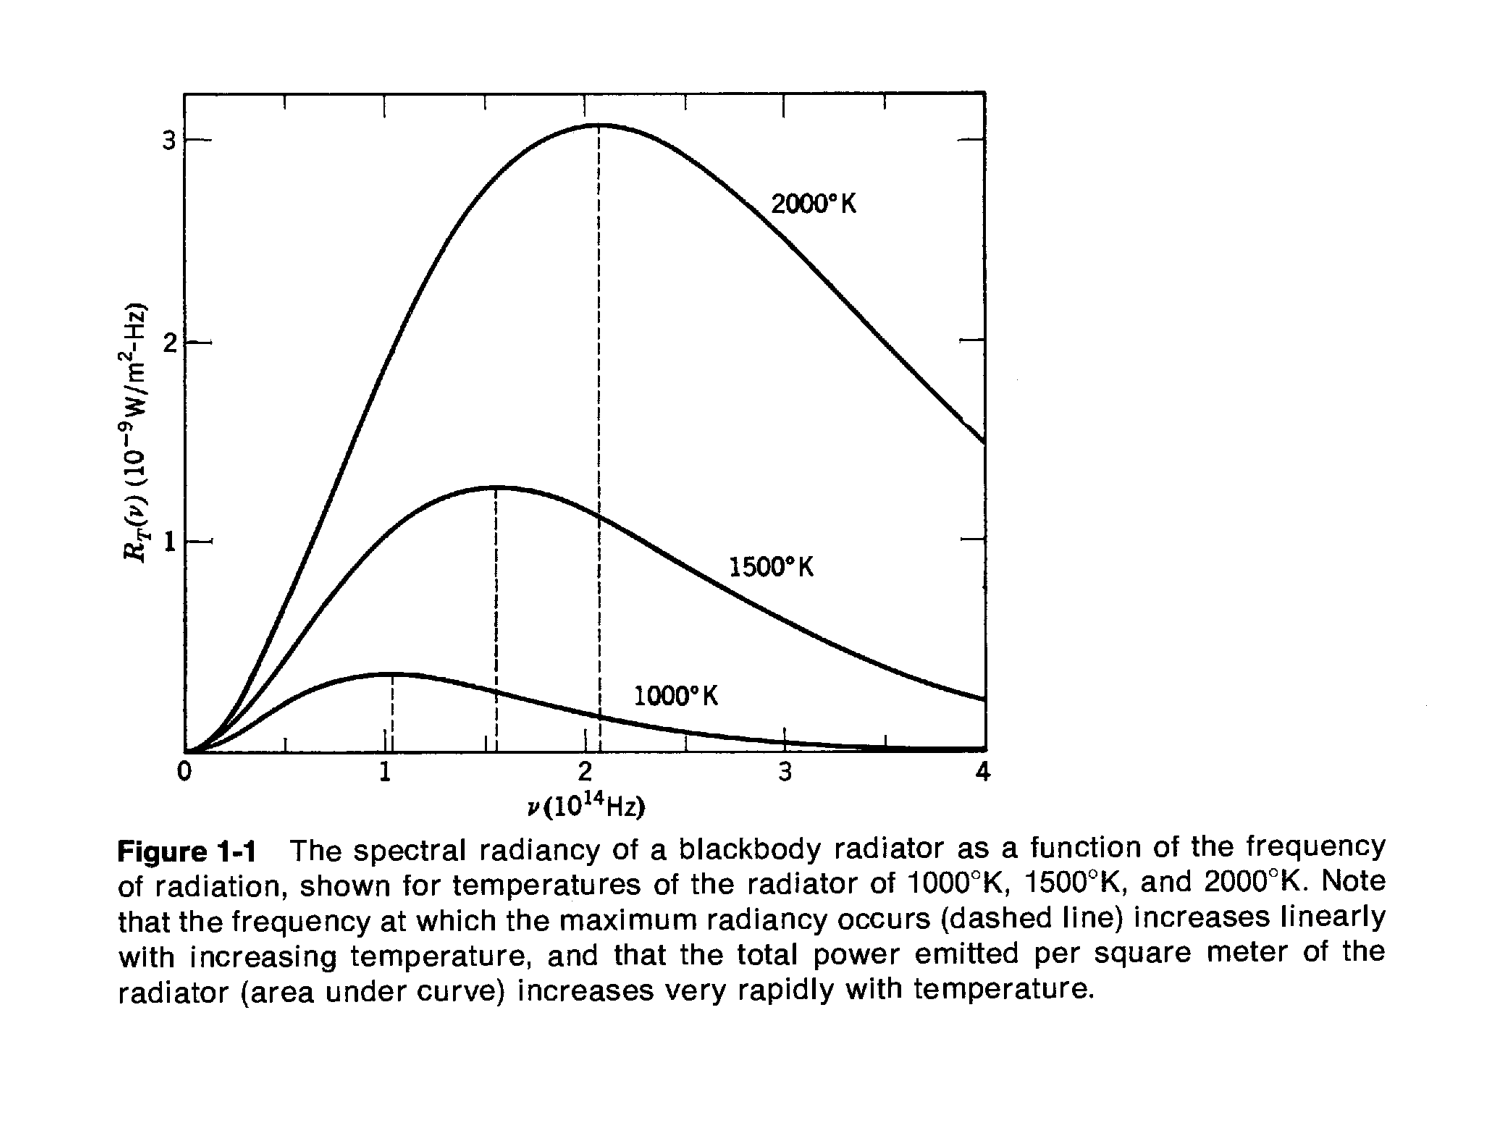
\includegraphics[scale=0.5]{/Spectral_radiancy}
\caption{Radianza spettrale di corpo nero a tre diverse temperature. Notare come il picco si sposti all'aumentare della temperatura.}
\end{figure}

Per descrivere la radiazione di corpo nero Rayleigh e Jeans utilizzarono (anche) le seguenti leggi empiriche:

la \textbf{legge di Stefan-Boltzmann}:
\begin{equation}
R_T = \sigma T^4
\end{equation}
che descrive la radianza totale in funzione della temperatura ed in cui compare la 
\begin{equation}
\mbox{\underline{costante di Stefan-Boltzmann}} \quad \sigma = 5.67 \cdot 10^{-8} \frac{W}{m^2 \cdot K^4}
\end{equation}

La \textbf{legge di spostamento di Wien} afferma che la frequenza/lunghezza d'onda di picco è proporzionale alla temperatura

\begin{equation}
\begin{split}
& \nu_{max} \propto T \\
& \mbox{ed usando la seguente relazione} \quad \lambda\nu = c \\
& \lambda_{max}T = \SI{2.898e-3}{mK}
\end{split}
\end{equation}

L'oggetto reale più simile al concetto teorico di corpo nero è la \underline{cavità di corpo nero}, cioè un oggetto cavo con pareti metalliche avente un piccolo buco sulla superficie: la radiazione che esce dal foro è interpretabile come corpo nero, vedi figura.

\begin{figure}[h]
\centering
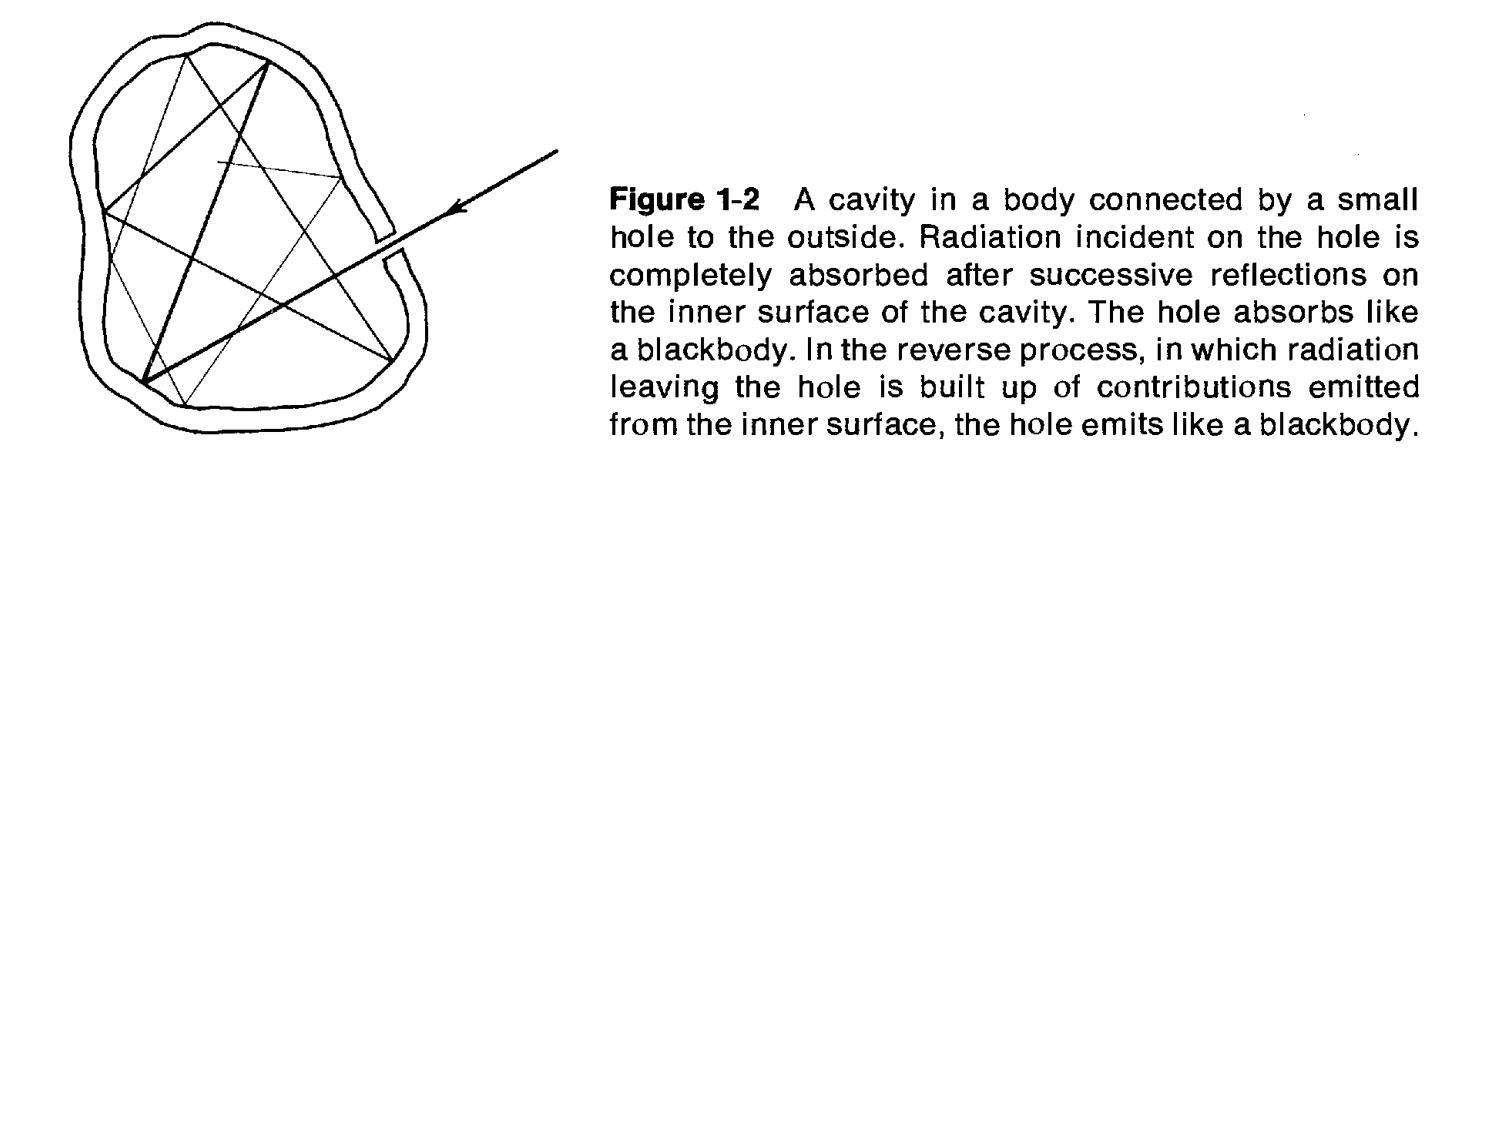
\includegraphics[scale=0.5]{/cavita_corponero}
\end{figure}

Introduciamo la \underline{\textbf{radiazione di cavità}} $\rho_T(\nu)$, che è la densità di energia contenuta in una unità di volume della cavità ad una certa temperatura $T$,
essa è ovviamente proporzionale alla Radianza totale, la cui derivazione è basata su ragionamenti puramente geometrici, in particolare la relazione è data da:
\begin{equation}
\frac{c}{4}\rho_T(\nu)=R_T(\nu)
\end{equation}

\subsection{Teoria classica di corpo nero di Rayleigh e Jeans}

A inizio '900 spiegare la forma dello spettro di corpo nero era uno dei problemi più dibattuti.
A dare un grande contributo furono Rayleigh e Jeans, che elaborarono la teoria classica di corpo nero, basandosi sulla fisica classica, per modellizzare la forma dello spettro di corpo nero.
Quindi si impegnarono nel trovare un modello teorico che potesse spiegare i risultati sperimentali.

Il ragionamento si divide in tre passaggi:
\begin{enumerate}[label=\Roman{*}.]
\item Le onde elettromagnetiche all'interno della cavità sono onde stazionarie?
\item Come contare il numero di onde stazionarie?
\item È possibile associare un'energia alle onde elettromagnetiche?
\end{enumerate}

\begin{figure}[h]
\centering
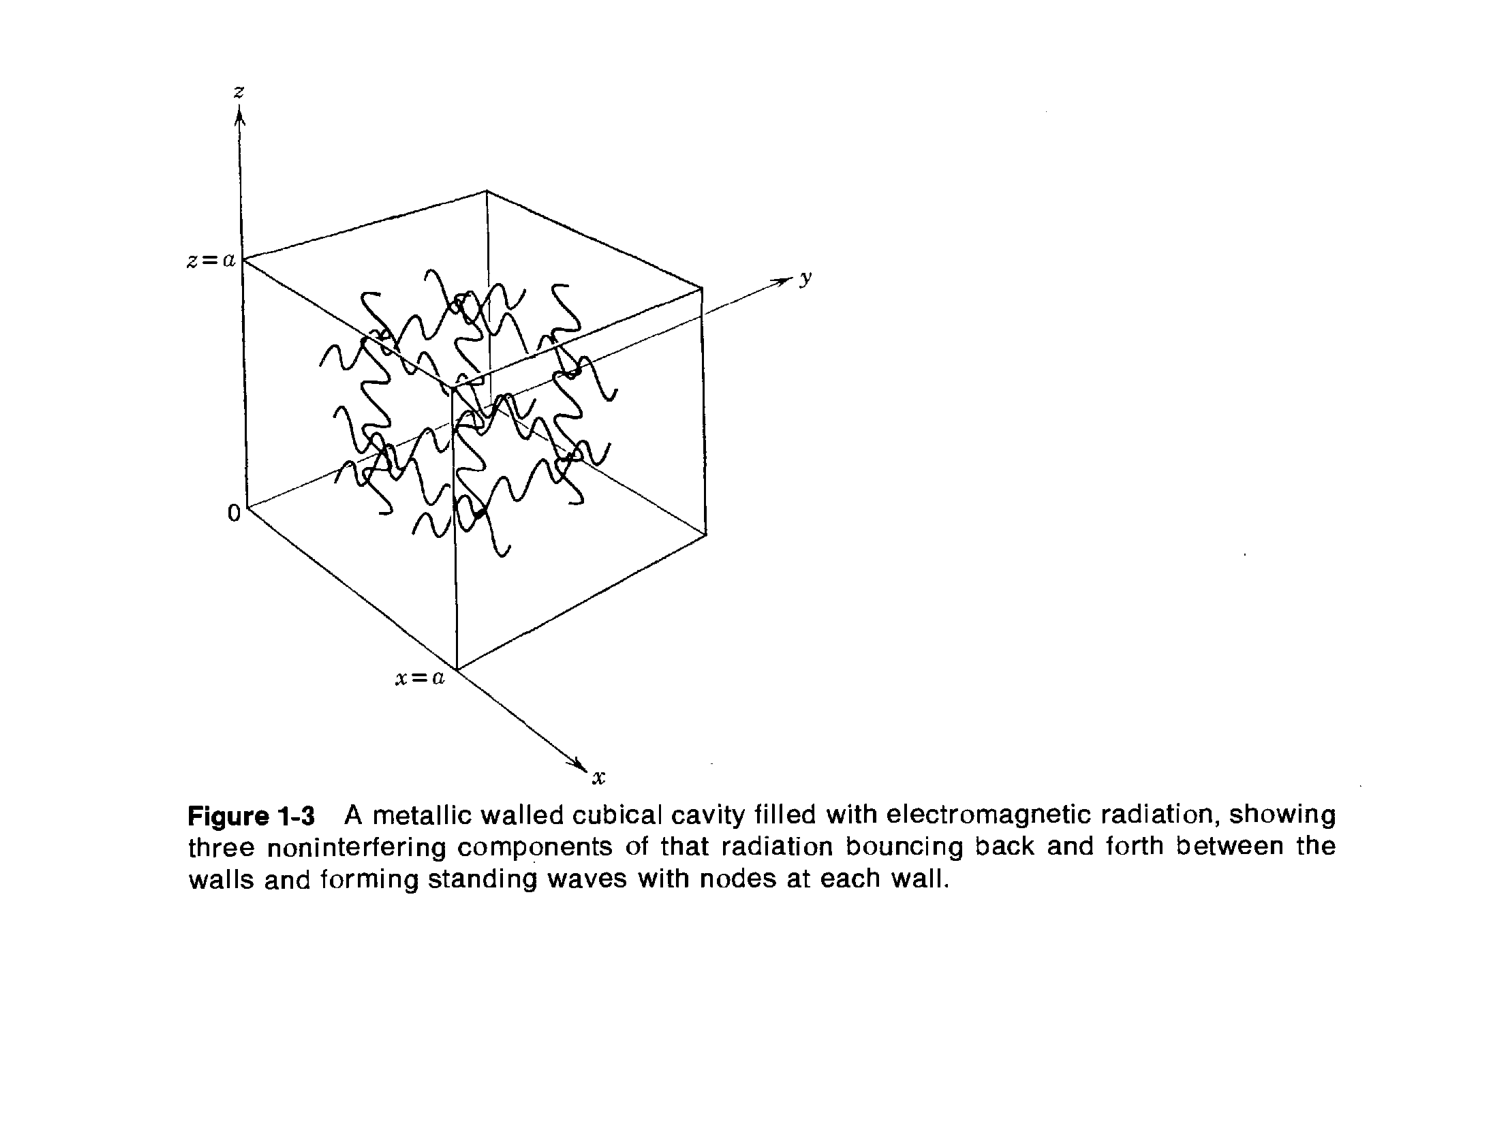
\includegraphics[scale=0.6]{/cubo_CorpoNero}
\caption{cubo Corpo Nero}
\end{figure}

Si consideri una cavità cubica e metallica riscaldata a temperatura $T$.
Essi ragionarono con le frequenze delle onde elettromagnetiche contenute nella cavità.
Vediamo in dettaglio i passaggi seguiti da Rayleigh e Jeans.

\begin{enumerate}[label=\Roman{*}.]

\item Prima di tutto occorre dimostrare che tali onde siano stazionarie.
Ogni onda può essere scomposta lungo le tre componenti spaziali e studiata indipendentemente. 
Consideriamo il lato del cubo $x \in (0, a)$.
La radiazione elettromagnetica è trasversale, cioè $\vec{E}$ campo elettrico è perpendicolare alla direzione di propagazione dell'onda, dunque il campo è parallelo alla parete, ma ciò porta, per il moto delle onde, all'annullarsi del campo $\vec{E}$ sulla parete, perciò deve esserci ampiezza nulla, e quindi $0$ e $a$ sono due nodi.
Dunque le onde sono stazionarie.

\begin{figure}[h]
\centering
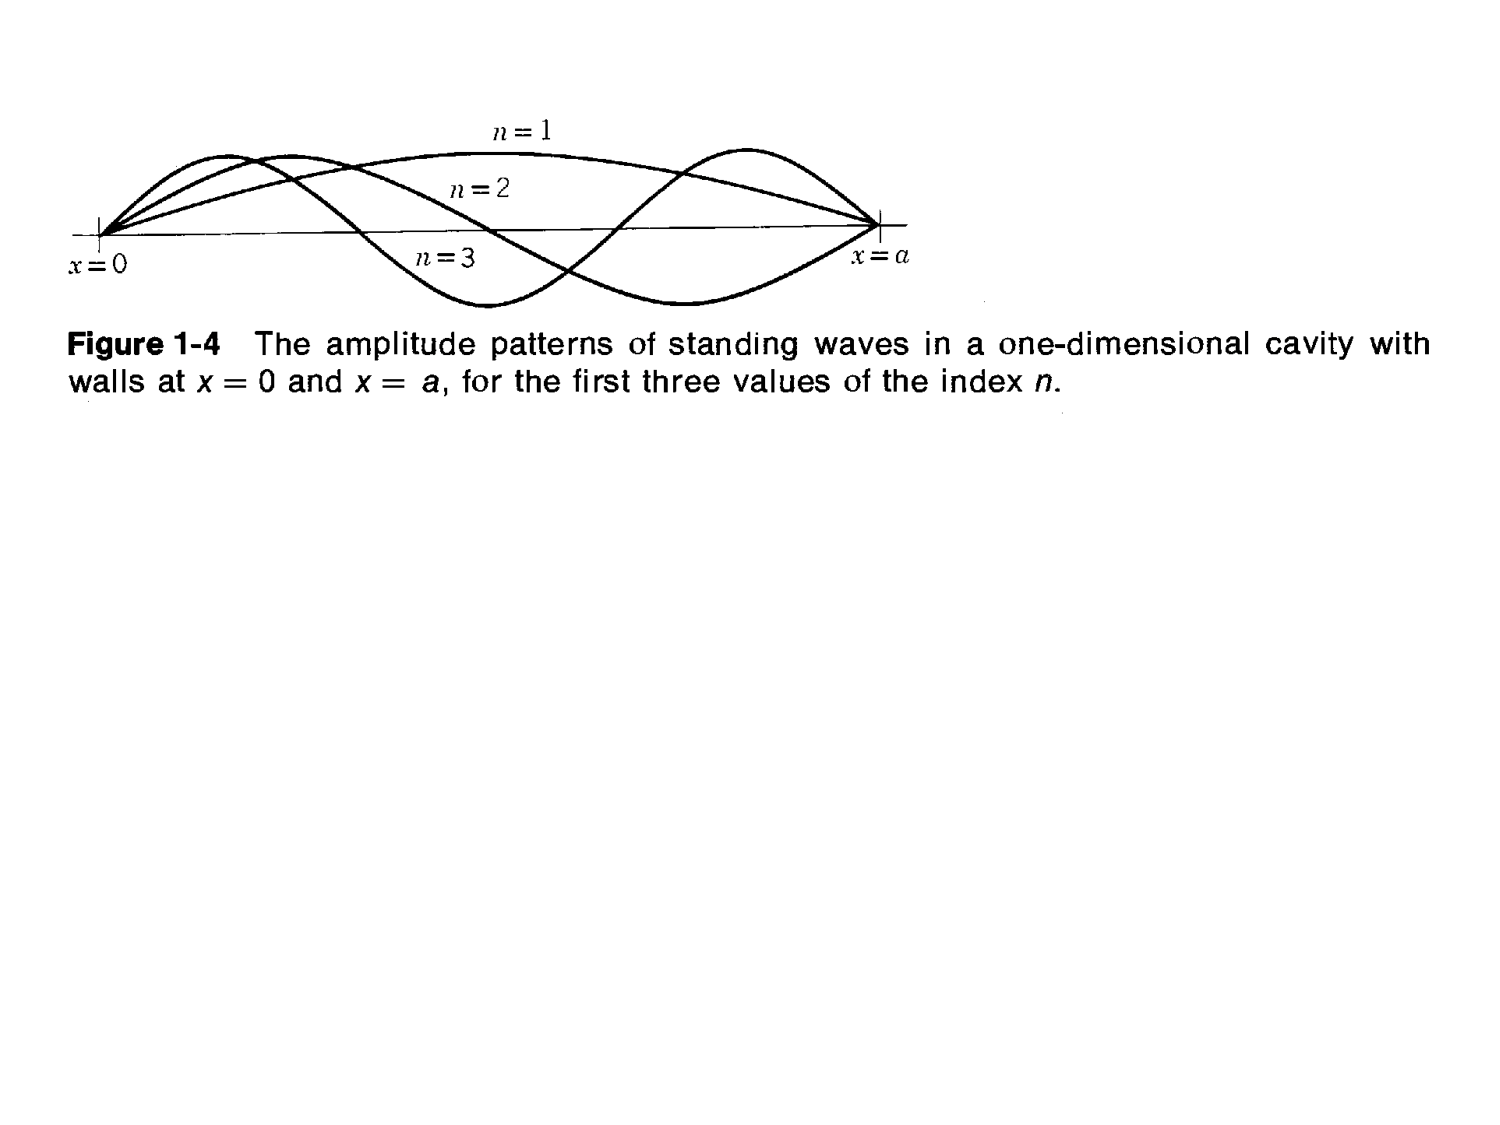
\includegraphics[scale=0.5]{/modiVibrazione}
\caption{modi vibrazione}
\end{figure}

\item Occorre contare il numero di onde, cominciamo dal caso 1-D lungo $x$
	
\begin{equation}
\begin{split}
& E(x, t) = E_0 \sin \Bigl(  \frac{2 \pi x}{\lambda}  \Bigr) \sin (2\pi \nu t) \\
& \frac{2x}{\lambda} = 0,1,2,3 ... = n \in \mathbb{N}
\end{split}
\end{equation}

Quindi $n=0$ corrisponde all'estremità, fissa, in $x=0$ e tutte le possibili onde stazionarie si trovano imponendo $x=a$:
\begin{equation}
\begin{split}
& \frac{ 2a}{\lambda } = n \quad\quad n = 1,2,3, ... \\
& \mbox{utilizzando la relazione} \quad \nu = \frac{c}{\lambda} \\
& \nu = \frac{ c n }{2a } \quad n = 1,2,3, ...
\end{split}
\end{equation}
Che sono quindi i valori permessi di frequenza per onde stazionarie.

\begin{figure}[h]
\centering
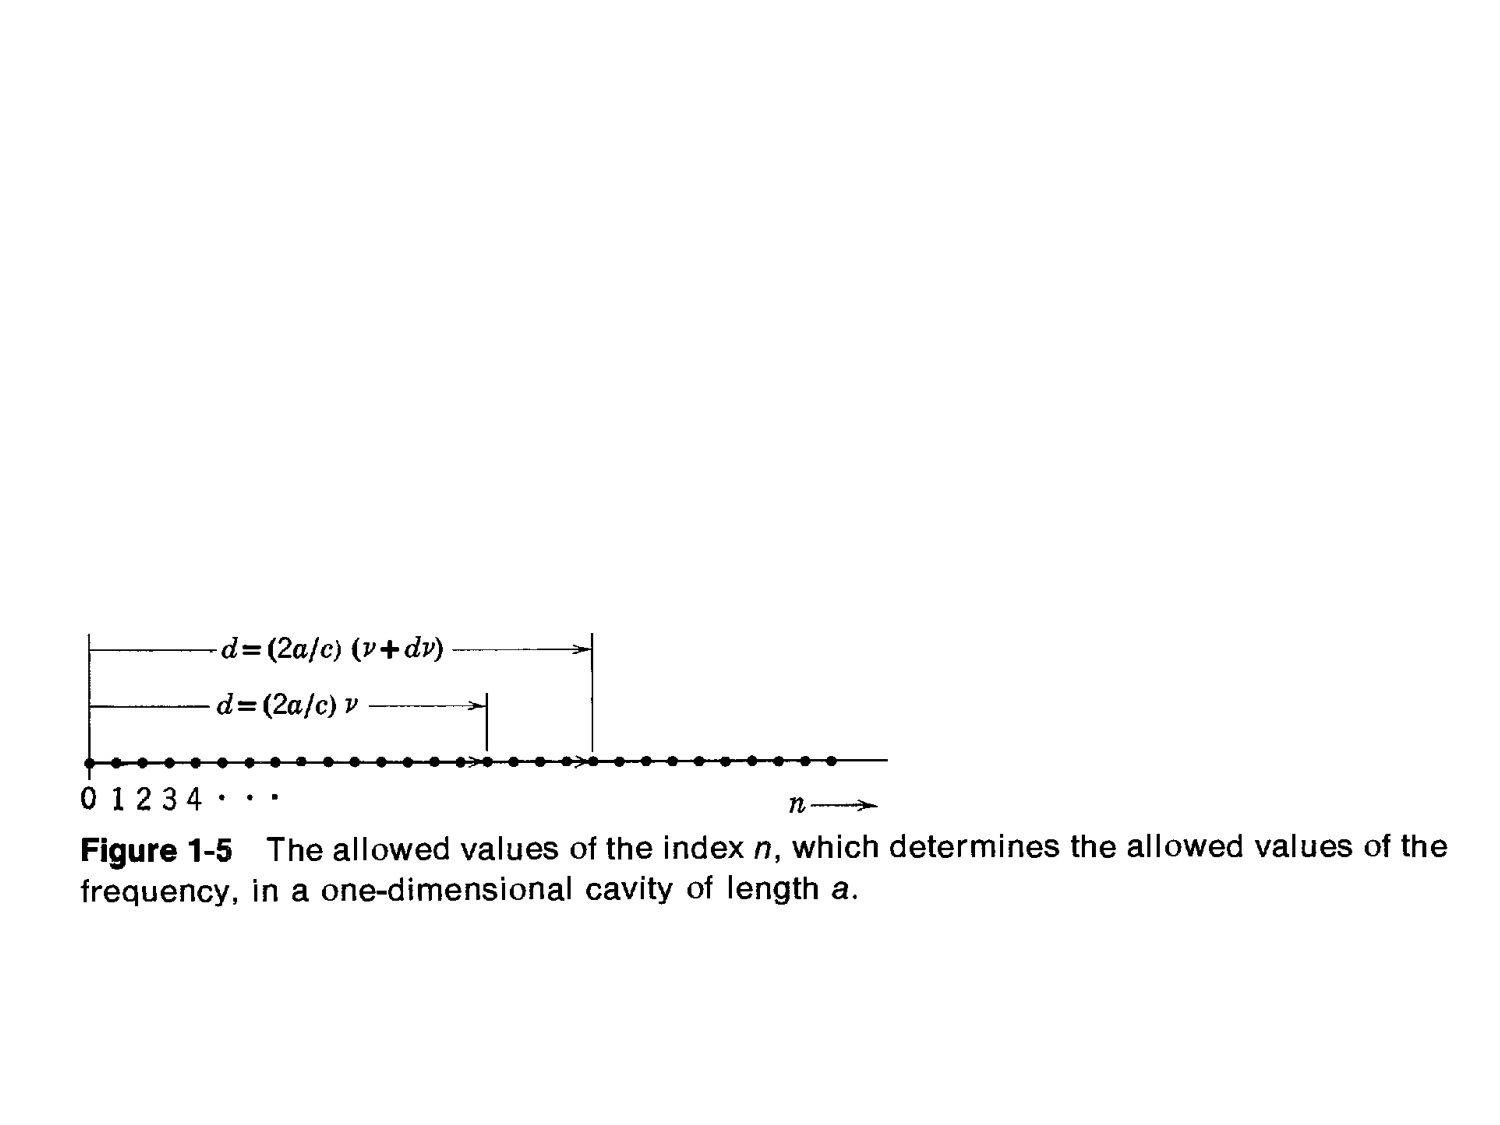
\includegraphics[scale=0.6]{/Blackbody_nodi}
\end{figure}
\begin{equation}
\begin{split}
& d = (\frac{ 2a}{c }) (\nu + d\nu) \quad - \quad d = (\frac{ 2a}{c }) \nu \\
& N(\nu)d\nu = 2 \Bigl(  \frac{2a}{c}  \Bigr) d\nu = \frac{4a}{c}d\nu 
\end{split}
\end{equation}
Nel caso unidimensionale questo è il numero di modi di vibrazione, dove il fattore 2 è dovuto al fatto che ci siano due possibili polarizzazioni $S$ e $P$. \\
\textbf{NB} Nel caso 1-D il numero di frequenze possibili non dipende da $\nu$.

Passiamo a 3 dimensioni, il valore di $n$ dipenderà ora da tre parametri $n_x, n_y, n_z \in \mathbb{N}$, da cui dipende anche il numero di frequenze permesse:
\begin{equation}
\begin{split}
& \frac{2a}{\lambda} = \sqrt{n_x^2 + n_y^2 + n_z^2} \\
& \nu = \frac{ c}{\lambda } = \frac{ c}{2a } \sqrt{n_x^2 + n_y^2 + n_z^2}
\end{split}
\end{equation}
\begin{figure}[h]
\centering
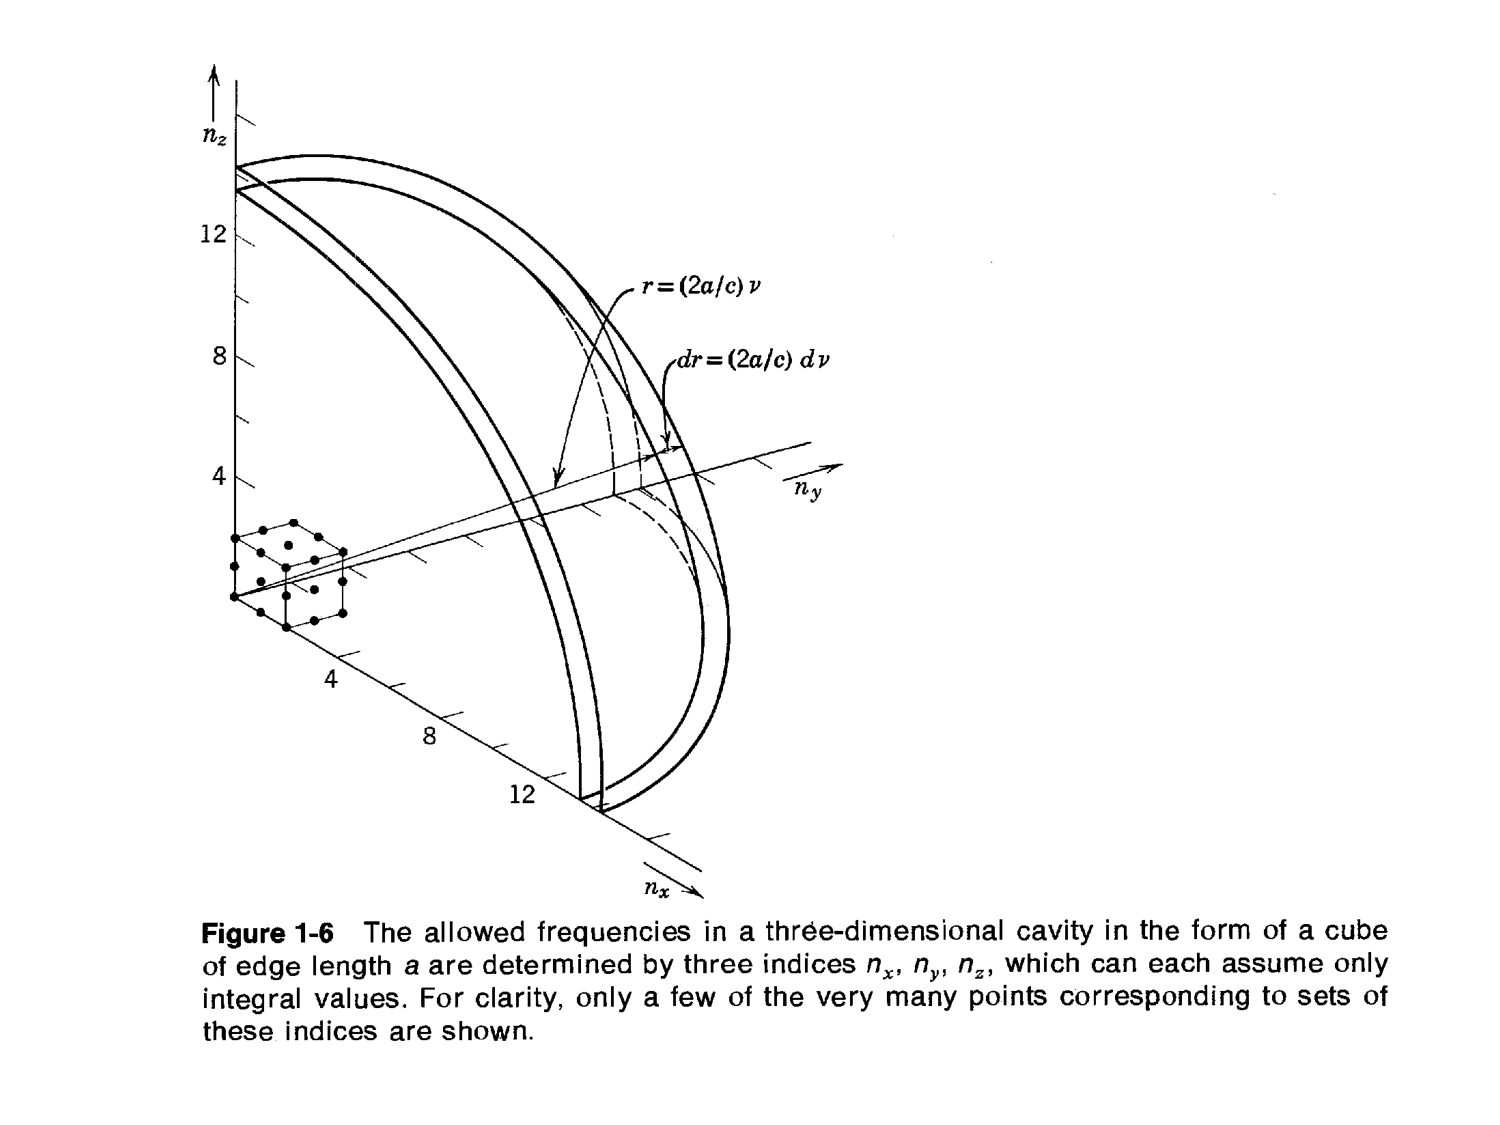
\includegraphics[scale=0.5]{/sfrera_nodi_permessi}
\caption{Numero di punti tra due shell a distanza $dr$, associati alle frequenze permesse}
\end{figure}

Conto quindi il numero di frequenze dal raggio $r$ al raggio $r + dr$:
\begin{equation}
\begin{split}
& N(\nu) d\nu = N(r)dr \\ 
& r = \frac{2a}{c}\nu \\
\end{split}
\end{equation}

ma il numero di punti nel volume dal raggio $r$ al raggio $r + dr$ è proprio il volume stesso, nel conto seguente utilizzo la sostituzione per $r$ appena trovata:
\begin{equation}
\begin{split}
& N(r) dr = \frac{ 1}{8 } 4 \pi r^2 dr = \frac{ \pi r^2 dr}{2 } \\
& N(\nu)d\nu = \frac{ \pi}{2 } \Bigl(  \frac{ 2a}{c }  \Bigr)^3 \nu^2 d\nu \\
& \mbox{che moltiplico x2 perché ho due stati di polarizzazione} \\
\Rightarrow & N(\nu) d\nu = \frac{ 8\pi V}{c^3 } \nu^2 d\nu
\end{split}
\end{equation}
ottengo così \underline{il numero di frequenze permesse} (modi di vibrazione) per le onde elettromagnetiche stazionarie all'interno della cavità di corpo nero, dove $V=a^3$ è il volume della cavità. \\
\textbf{NB} Nel caso 3-D il numero di frequenze possibili dipende da $\nu$.


\item Stima dell'energia media di ogni onda stazionaria di frequenza $\nu$.
Se ho un sistema di particelle in equilibrio termico, l'energia cinetica media per molecola per grado di libertà è, dalla legge di equipartizione dell'energia:
\begin{equation}
\begin{split}
\bar \varepsilon = \frac{ 1}{2 } & k T \\
\mbox{costante di Boltzmann } & k = \SI{1.3806e-23}{J/K}
\end{split}
\end{equation}
Considerando le onde come oggetti oscillanti devo tenere in considerazione anche l'energia potenziale, con argomentazioni di fisica classica, trovo l'energia media totale:
\begin{equation}
\bar \varepsilon = k T
\end{equation}
Avendo stimato l'energia si ottiene la formula classica di Rayleigh Jeans per il corpo nero 
\begin{equation}
\rho_T(\nu)d\nu = \frac{8 \pi \nu^2 k T }{c^3}d\nu
\end{equation}
Quello che faccio è moltiplicare il numero di onde stazionarie all'interno della cavità 
$$\frac{8 \pi \nu^2}{c^3}$$
per l'energia media di ogni onda stazionaria
$$kT$$
dividendo per il volume $V$, per ottenere la \underline{densità di energia} $\rho_T$ all'interno della cavità di corpo nero.
La teoria classica di corpo nero è verificata solo per valori piccoli di $\nu$ e si discosta rapidamente dai dati sperimentali, servirebbe una teoria che faccia dipendere l'energia media dalla frequenza.
\begin{figure}[h]
\centering
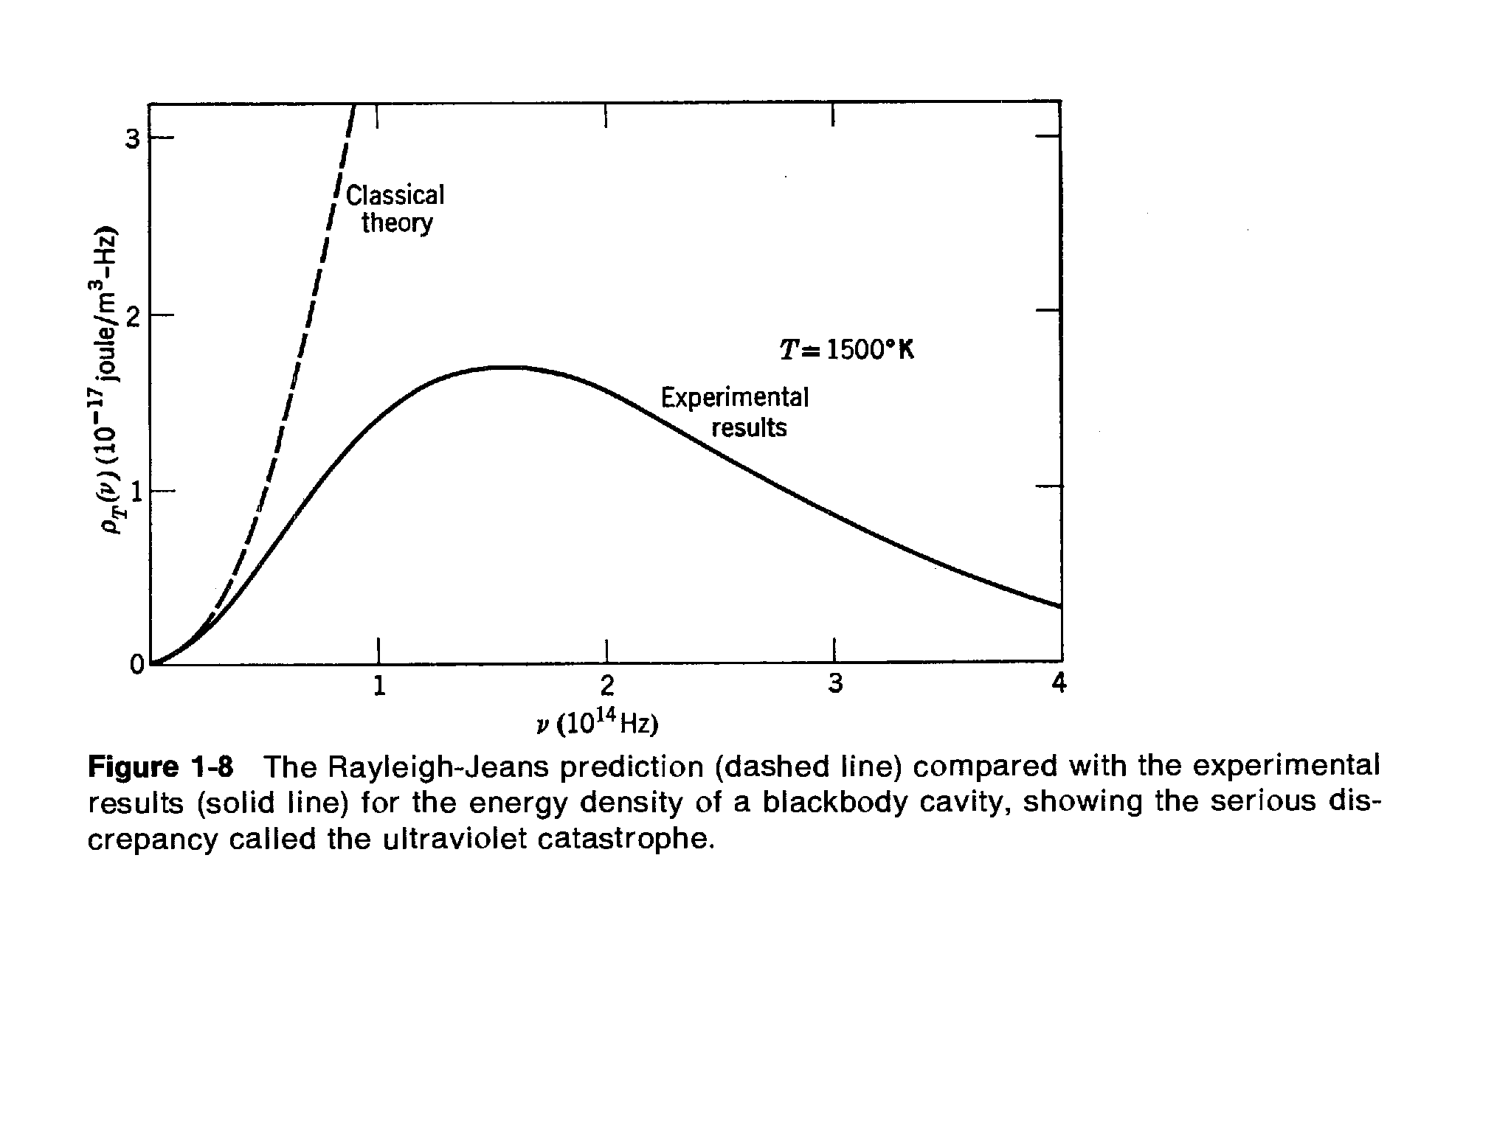
\includegraphics[scale=0.5]{/catastrofe_ultravioletta}
\caption{Catastrofe ultravioletta}
\end{figure}

\end{enumerate}

\subsection{Statistica classica di Boltzmann}
Introduciamo la legge statistica classica di Boltzmann (o di Maxwell-Boltzmann) come la probabilità $P$ di trovare una certa entità di un sistema con energia nell'intervallo tra $\varepsilon$ e $\varepsilon+d\varepsilon$, data dalla formula

\begin{equation}
P(\varepsilon)d\varepsilon = c e^{ -\frac{\varepsilon}{kT } }
\end{equation}
Tale formula è valida quando il numero degli stati di energia \underline{non} dipende da $\varepsilon$, valida quindi ad esempio per l'oscillatore armonico unidimensionale.

La costante $c$ si calcola imponendo che l'integrale su tutto lo spettro di energie sia pari a $1$:
\begin{equation}
\begin{split}
\int_{0}^{\infty} P(\varepsilon) d\varepsilon & = c \int_{0}^{\infty} e^{ -\frac{\varepsilon}{kT } } d\varepsilon = 1 \\
c & = \frac{ 1}{kT }
\end{split}
\end{equation}

Per cui si trova la formula che descrive la statistica classica di Boltzmann 
\begin{equation}
P(\varepsilon) = \frac{ e^{ - \frac{\varepsilon}{kT } } }{kT }
\end{equation}

Applico questa statistica agli elementi del set di onde stazionarie oscillanti nella cavità di corpo nero, quindi l'energia media è data da: 
a numeratore l'energia $\varepsilon$ moltiplicata (pesata) per la probabilità che l'entità abbia quell'energia (integrata su tutti i valori di energia), 
a denominatore ho la probabilità di trovare l'entità con qualsiasi energia (integrata su tutti i valori di energia)
\begin{equation}
\begin{split}
& \bar\varepsilon=\frac{\int_{0}^{\infty} \varepsilon P(\varepsilon)\,d\varepsilon}{\int_{0}^{\infty} P(\varepsilon)\,d\varepsilon} = \frac{\int_{0}^{\infty} \varepsilon \frac{ e^{ - \frac{\varepsilon}{kT } } }{kT } d\varepsilon}{\int_{0}^{\infty} \frac{ e^{ - \frac{\varepsilon}{kT } } }{kT }d\varepsilon} \\
& \mbox{ pongo } \beta=\frac{1}{kT} \\
& \bar\varepsilon= \frac{\int_{0}^{\infty} \varepsilon e^{ - \beta \varepsilon } d\varepsilon}{\int_{0}^{\infty} e^{ - \beta \varepsilon } d\varepsilon} = - \frac{ d}{d\beta } \ln \int_0^{\infty} e^{ -\beta \varepsilon } d\varepsilon = - \frac{ d}{d\beta } \ln \frac{ 1}{\beta } \\
& \bar\varepsilon= \beta \frac{ 1}{\beta^2 } = \frac{ 1}{\beta } = kT
\end{split} 
\end{equation}
Ottenendo così il risultato, utilizzato anche in precedenza: l'energia media è $\bar \varepsilon = kT$, per cui si ha la catastrofe ultravioletta.

\subsection{Ipotesi quantica di Planck e formula di Planck per il corpo nero}

Planck ipotizza che l'energia non possa assumere tutti i valori ma solo valori discreti
$$\varepsilon = 0,\Delta\varepsilon,2\Delta\varepsilon,3\Delta\varepsilon, ...$$

Per cui per misurare l'area del sottografico, e quindi la Radianza totale, non occorrerà più eseguire un integrale ma piuttosto una sommatoria su tutti i "rettangolini" discreti.

\begin{figure}[h]
\centering
\includegraphics[scale=0.5]{/ipotesi_quantica_Planck}
\caption{Ipotesi quantica di Planck}
\end{figure}

\begin{figure}[h]
\centering
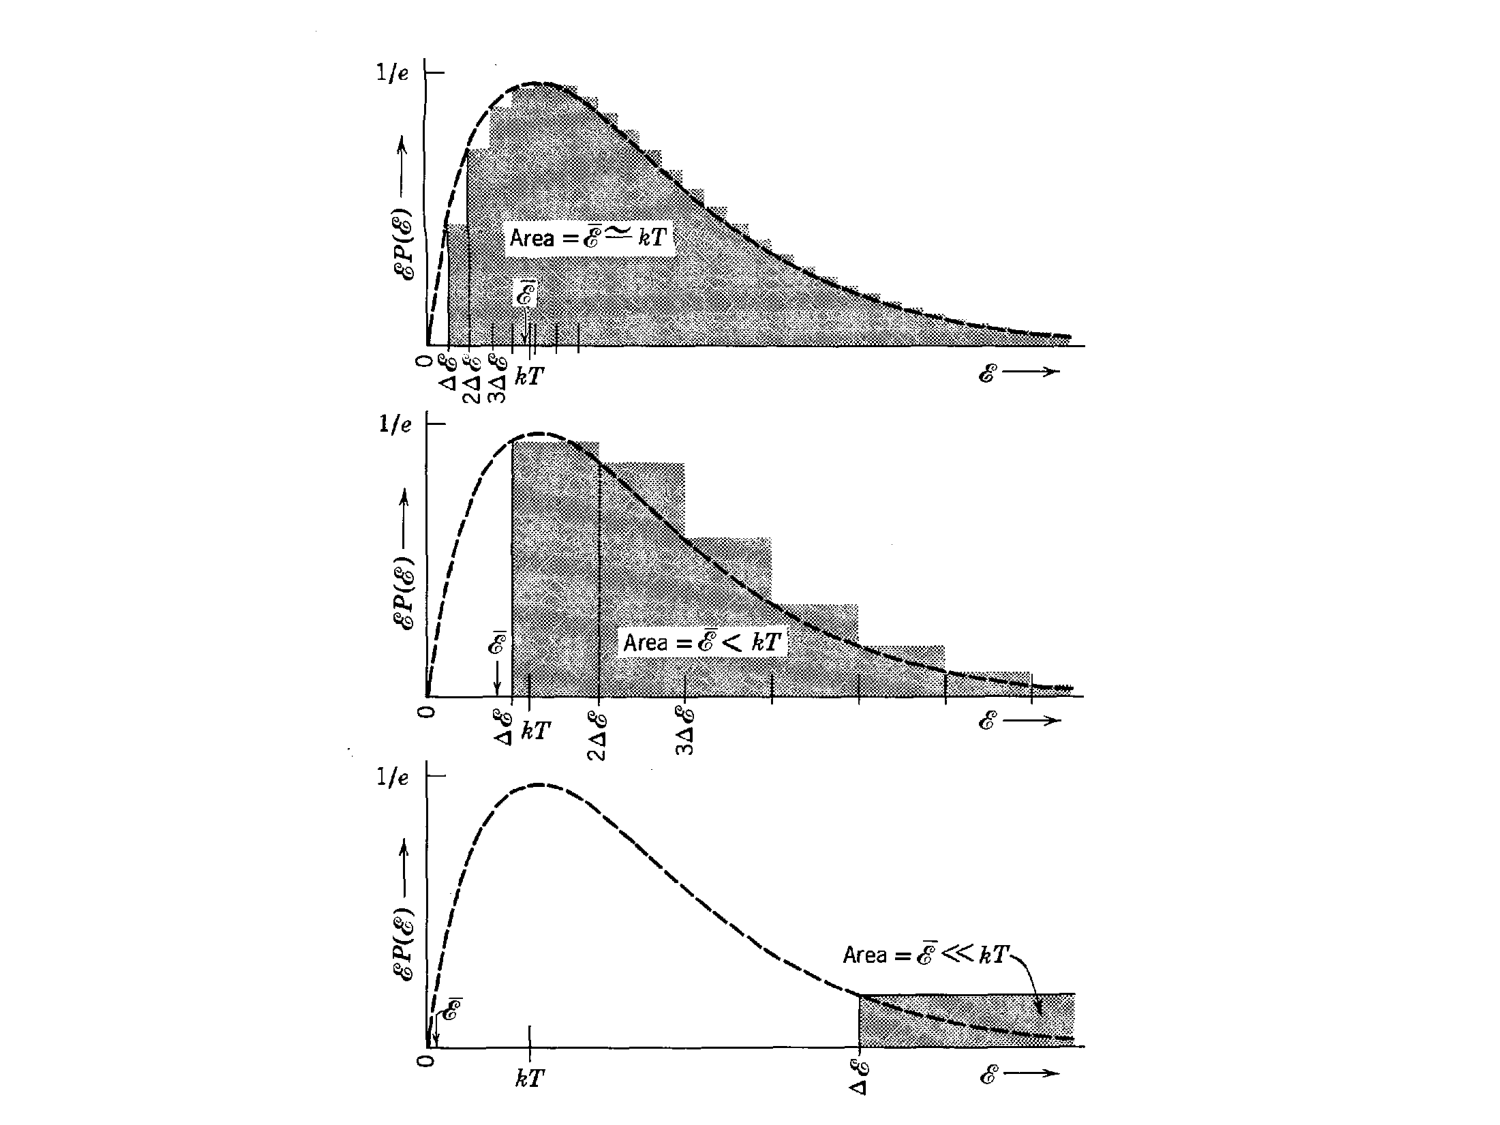
\includegraphics[scale=0.5]{/rettangolini}
\caption{Sommatoria sui rettangolini del sottografico}
\end{figure}

Analizzando l'andamento di $\bar\varepsilon$ in funzione di $\Delta\varepsilon$ si trova l'espressione:
\begin{equation}
\bar\varepsilon = \frac{ \Delta\varepsilon}{e^{ \frac{ \Delta\varepsilon}{kT } } - 1 }
\end{equation}
Per cui
\begin{equation}
\begin{split}
& se \quad \Delta\varepsilon \rightarrow 0 \quad \Rightarrow \quad \bar\varepsilon \sim \frac{ 2 k^2 T^2 }{2kT + \Delta\varepsilon } \rightarrow kT  \quad \mbox{dove } e^x \sim 1 + x + \frac{ x^2}{2 } \\
& se \quad \Delta\varepsilon = kT \quad \Rightarrow \quad \bar\varepsilon = \frac{ kT }{ e - 1 } < kT \\
& se \quad \Delta\varepsilon \rightarrow \infty \quad \Rightarrow \quad \bar\varepsilon = \lim_{\Delta\varepsilon = \infty}  \frac{ \Delta\varepsilon}{e^{ \frac{ \Delta\varepsilon}{kT } } - 1 } = 0
\end{split}
\end{equation}

Quindi il risultato classico $\bar\varepsilon = kT$ è utile solo per $\Delta\varepsilon = h\nu \rightarrow 0$ ovvero per frequenze $\nu$ piccole.

La soluzione si trova se si mettono in correlazione $\Delta\varepsilon \propto \nu$ oppure scrivendo $\Delta\varepsilon = h\nu$ dove $h=\SI{6.63e-34}{J.s}$ è la Costante di Planck.
La \underline{quantizzazione dell'energia}, quindi i valori possibili dell'energia, si scrive come $n h \nu$ con $n = 0,1,2, ...$

L'espressione della probabilità $P(\varepsilon)$ è la stessa legge statistica classica
\begin{equation}
\begin{split}
& P(\varepsilon) = \frac{ e^{ -\frac{ \varepsilon}{ kT} }}{kT } \\
& \bar\varepsilon = \frac{ \sum_{n=0}^{\infty} \varepsilon P(\varepsilon)}{\sum_{n=0}^{\infty} P(\varepsilon) } \quad\quad \varepsilon= n h\nu \quad n=0,1,2, ... \\
& \bar\varepsilon = \frac{ \sum_{n=0}^{\infty}  \frac{ nh\nu}{kT } e^{ -\frac{ nh\nu}{kT } }  }{\sum_{n=0}^{\infty} \frac{ 1 }{kT } e^{ -\frac{ nh\nu}{kT } } } =
kT \frac{\sum_{n=0}^{\infty} n\alpha e^{ -n\alpha } }{\sum_{n=0}^{\infty} e^{ -n\alpha } } \quad\quad \alpha = \frac{ h\nu}{kT }
\end{split}
\end{equation}

A questo punto si procede come nel caso precedente, introducendo la seguente catena di uguaglianze

\begin{equation}
\begin{split}
& - \alpha \frac{ d}{d\alpha } \ln \sum_{n=0}^{\infty} e^{-n\alpha} = \frac{ - \alpha \frac{ d}{d\alpha } \sum_{0}^{\infty} e^{-n\alpha} }{ \sum_{0}^{\infty} e^{-n\alpha}} = 
\frac{ - \sum_{0}^{\infty} \alpha \frac{ d}{d\alpha } e^{-n\alpha} }{ \sum_{0}^{\infty} e^{-n\alpha}} = \frac{\sum_{0}^{\infty} n\alpha e^{ -n\alpha } }{\sum_{0}^{\infty} e^{ -n\alpha } } \\
& \mbox{sostituendo si ottiene } \\
& \bar\varepsilon = kT \Bigl(  - \alpha \frac{ d}{d\alpha } \ln \sum_{n=0}^{\infty} e^{ -n\alpha }  \Bigr) = -h\nu \frac{ d}{d\alpha } \ln \sum_{n=0}^{\infty} e^{ -n\alpha } \\
& \sum_{n=0}^{\infty} e^{ -n\alpha } = 1 + e^{ -\alpha } + e^{ -2\alpha } + ... = 1 + x + x^2 + ... = \frac{ 1}{1-x }\\
& \mbox{utilizziamo ora la serie geometrica per eseguire la derivata e si scrive il risultato come} \\
& \bar\varepsilon = - h\nu \Bigl[ - \frac{ e^{ -\alpha }}{1 - e^{ -\alpha } } \Bigr] = \frac{ h\nu}{ e^{ \alpha } - 1 } = \frac{ h\nu}{ e^{ \frac{ h\nu}{kT } } - 1} 
\end{split}
\end{equation}

Quindi l'espressione finale dell'energia media nella cavità è
\begin{equation}
\bar\varepsilon = \frac{ h\nu}{ e^{ \frac{ h\nu}{kT }} - 1} 
\end{equation}

Per ottenere \underline{l'espressione della radiazione di cavità} moltiplico il numero di modi di vibrazione possibili per un'onda stazionaria all'interno della cavità
$$\frac{ 8\pi\nu^2}{c^3 }$$
per l'espressione dell'energia media di ogni onda stazionaria nella nuova ipotesi di Planck, ottengo quindi

\begin{equation}
\rho_T(\nu) d\nu = \frac{ 8\pi\nu^2}{c^3 } \frac{ h\nu}{ e^{ \frac{ h\nu}{kT }} - 1} d\nu
\end{equation}

anche detta \textbf{Formula di Planck per il corpo nero (1900)}, tale formula è in perfetto accordo con i dati sperimentali.
Questo risultato da inizio alla fisica moderna, introducendo il concetto di energia quantizzata inizia quindi la meccanica quantistica.

Cerchiamo ora un'espressione analoga in funzione di$\lambda$
$$\rho_T(\lambda) d\lambda = -\rho_T(\nu)d\nu $$

considero che
$$\nu = \frac{ c}{\lambda } \quad \Rightarrow \quad d\nu = -\Bigl(  \frac{ c}{\lambda^2 }  \Bigr) d\lambda \quad \Rightarrow \quad \frac{ d\nu}{d\lambda } = -\Bigl(  \frac{ c}{\lambda^2 }  \Bigr) $$

quindi sostituendo in questo modo
$$\rho_T(\lambda) = -\rho_T(\nu) \frac{ d\nu}{d\lambda } = -\rho_T(\nu) \frac{ c}{\lambda^2 }$$

si ottiene l'espressione cercata
\begin{equation}
-\rho_T(\lambda) d\lambda = \frac{ 8\pi h c }{\lambda^5 } \frac{ d\lambda}{e^{ \frac{ hc}{\lambda k T } } -1 }
\end{equation}

\begin{figure}[h]
\centering
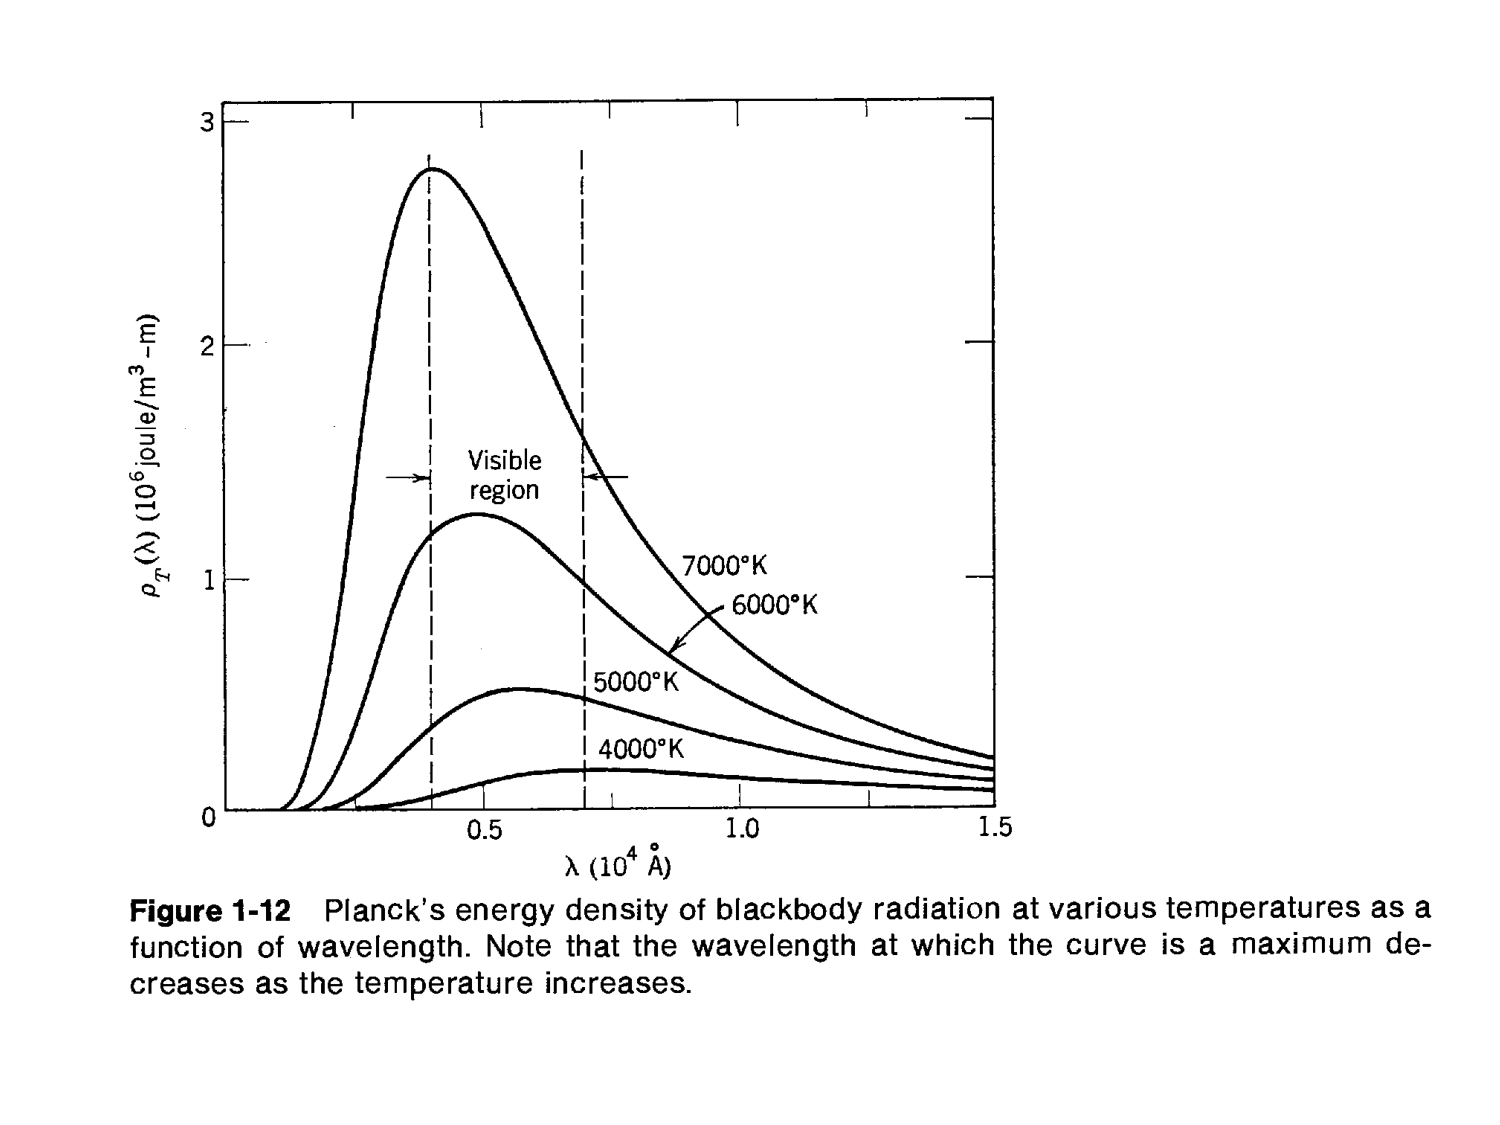
\includegraphics[scale=0.5]{/spettri_corponero}
\caption{Vari spettri di corpo nero}
\end{figure}

\paragraph{Derivazione della legge di Stefan}
Come si arriva alla formula di Stefan-Boltzmann partendo dalla formula di Planck per il corpo nero?
Ricordo che esiste le relazioni
$$\frac{ c}{4 } \rho_T(\nu) = R_T(\nu) \quad e \quad R_T = \int_0^{\infty} R_T(\nu)d\nu$$
quindi
\begin{equation}
\begin{split}
& \rho_T(\nu) d\nu = \frac{ 8\pi\nu^2}{c^3 } \frac{ h\nu}{ e^{ \frac{ h\nu}{kT }} - 1} d\nu \\
& R_T = \int_0^{\infty} \frac{ 2\pi h}{c^2 } \frac{ \nu^3}{e^{ \frac{ h\nu}{kT } } - 1 } d\nu \\
& R_T = \frac{ 2\pi h}{c^2 } \Bigl(  \frac{ kT}{h }  \Bigr)^4 \int_0^{\infty} \frac{ x^3}{e^x - 1 }dx \quad \mbox{dove} \quad x=\frac{ h\nu}{kT }\\
& \mbox{integrale noto} \quad \int_0^{\infty} \frac{ x^3}{e^x - 1 }dx = \frac{ \pi^4}{15 } \\
& R_T = \sigma T^4 \quad \mbox{dove} \quad \mbox{dove}\quad \sigma = \frac{ 2\pi^5 k^4}{15 h^3 c^2 } \simeq \SI{5.676e-8}{W / m^2 K^4}
\end{split}
\end{equation}

\paragraph{Postulato di Planck:} ogni entità fisica con un grado di libertà la cui "coordinata" è una funzione sinusoidale del tempo può avere solo energia totale $E$ tale che sia soddisfatta la relazione $\varepsilon = n h \nu$ con $n=0,1,2, ...$.
Il postulato di Planck si estende quindi a tutte le entità fisiche modellizzabili come oscillatori armonici semplici.

\begin{figure}[h]
\centering
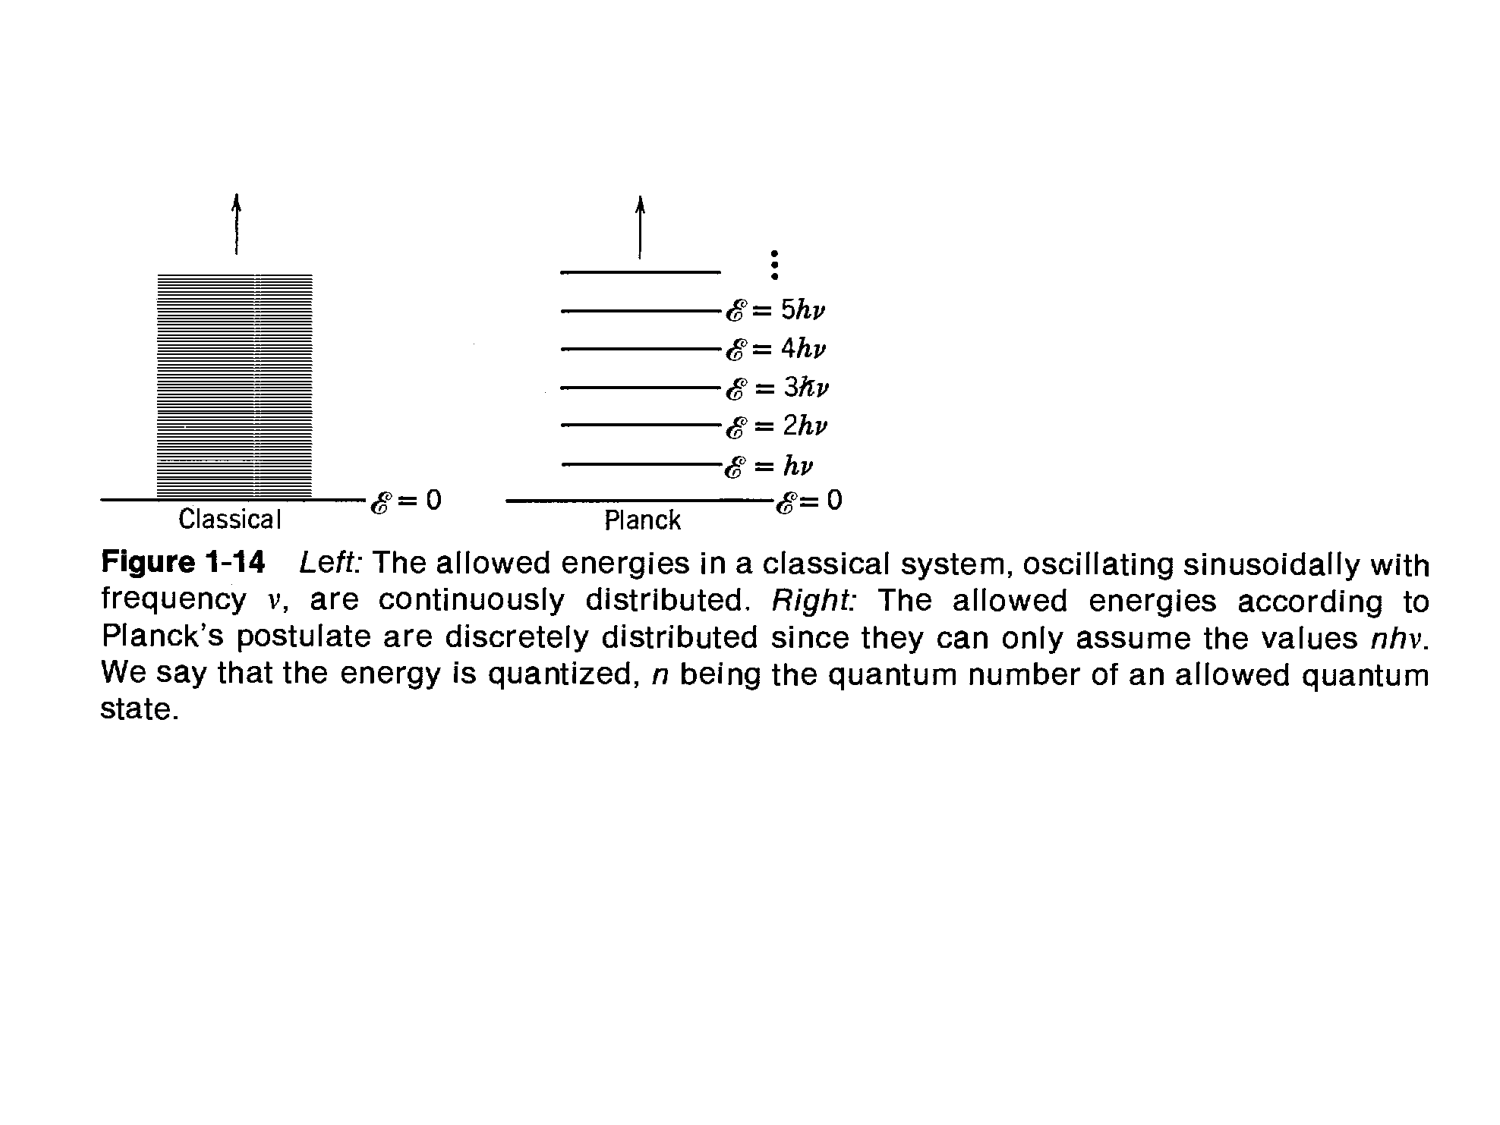
\includegraphics[scale=0.5]{/energia_quantizzata}
\caption{Confronto grafico tra la trattazione classica e quella quantizzata proposta da Planck}
\end{figure} 

\newpage

\paragraph{Esercizio}

Si consideri una massa puntiforme $m=\SI{0.01}{kg}$ appesa ad un filo di lunghezza $l=\SI{0.1}{m}$ e sia $\theta=\SI{0.1}{rad}$ l'angolo massimo di oscillazione. L'energia di questo pendolo appare continua o quantizzata? \\

Soluzione:
utilizzando risultati di fisica classica, calcolo la frequenza di questo pendolo
\begin{equation}
\nu = \frac{ 1}{2\pi } \sqrt{\frac{ g}{l }} = \frac{ 1}{2\pi }\sqrt{\frac{ \SI{9.81}{m/s^2}}{\SI{0.1}{m} }} = \SI{1.6}{Hz}
\end{equation}

e calcolo l'energia potenziale del pendolo
\begin{equation}
mgh = mgl(1-\cos \theta) = \SI{0.01}{kg} \cdot \SI{9.81}{m/s^2} \cdot \SI{0.1}{m} \cdot (1-\cos \theta) = \SI{5e-5}{j}
\end{equation}

Il quanto di energia che posso associare a questo pendolo 
\begin{equation}
\Delta E = h\nu = \SI{6.63e-34}{j.s} \cdot \SI{1.6}{Hz} = \SI{e-33}{j}
\end{equation}
nell'ipotesi che l'energia del pendolo sia quantizzata.
Ottengo un numero molto piccolo rispetto all'energia complessiva del pendolo, per cui il rapporto
\begin{equation}
\frac{ \Delta E }{E } = \SI{2e-29}{}
\end{equation}
Possiamo renderci conto della quantizzazione solo quando il quanto $\Delta E$ e l'energia $E$ sono grandezze confrontabili.

Da cui si vede come la fisica classica offra un'ottima approssimazione per lo studio di problemi di questo tipo.




    %%
%% Author: dariochinelli
%% 2020-09-29
%%


\section{Effetto fotoelettrico}
È uno dei possibili processi di interazione tra la radiazione elettromagnetica e la materia, come anche l'effetto Compton che vedremo più avanti. La radiazione elettromagnetica non ha solo la natura ondulatoria ma anche la natura particellare, questi effetti sono una manifestazione di questa natura particellare.

\paragraph{Esperimenti di Hertz}
Nel 1887 Hertz, studiando la scarica dei conduttori elettrizzati stimolata da una scintilla elettrica nelle vicinanze,
si accorse che tale fenomeno è più intenso se gli elettrodi vengono illuminati con luce ultravioletta.

\subsection{Esperimento di Lenard}
La \underline{scoperta} dell'effetto fotoelettrico viene attribuita a Lenard.
Scopre che il motivo dell'osservazione di Hertz è che degli elettroni vengono emessi dal catodo (elettrodo negativo) quando si fa incidere su di esso della radiazione elettromagnetica, in particolare gli esperimenti erano fatti con luce visibile e ultravioletta.
\textbf{Apparato sperimentale:} tubo di vetro sotto vuoto che contiene due elettrodi a cui viene applicata una differenza di potenziale, della luce viene fatta incidere su un elettrodo (negativo) da cui fuoriescono elettroni (fotoelettroni) attirati verso l'elettrodo positivo.
 L'emissione di elettroni viene rilevata come una corrente misurata con un amperometro.

\begin{figure}[h]
\centering
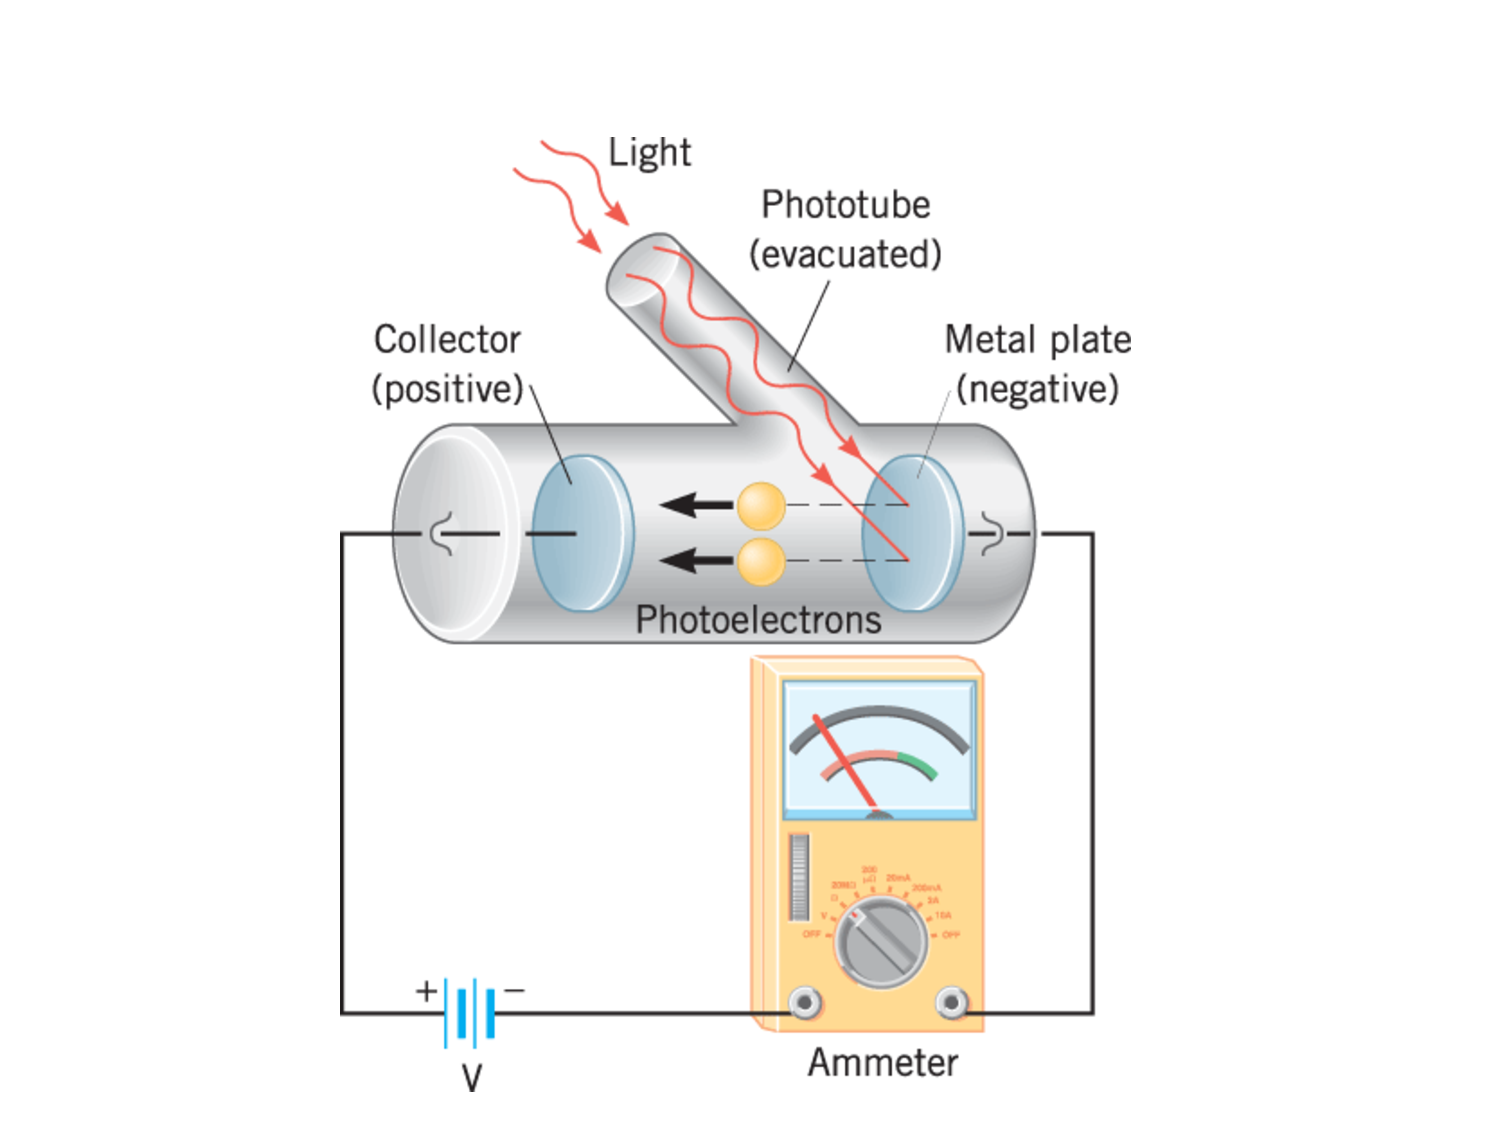
\includegraphics[scale=0.5]{/Schema_EffettoFotoelettrico}
\caption{Schema dell'esperimento di Lenard del 1900}
\end{figure}

\textbf{Risultati sperimentali} \\
\underline{il primo risultato sperimentale} è la corrente misurata in funzione del potenziale applicato (vedi grafico a sinistra in figura \ref{risultati_Lenard}).
Fissata l'intensità della luce incidente al valore $I_a$, quando il potenziale che applico è elevato la corrente raggiunge un livello di saturazione, riesco a raccogliere quindi tutti i fotoelettroni uscenti dal catodo.
Se porto a zero il potenziale la corrente non si annulla e nemmeno se applico un potenziale negativo. 
Significa che i fotoelettroni emessi hanno una certa energia cinetica e anche invertendo la polarità dei due elettrodi, pur venendo in parte respinti, sono ancora in grado di raggiungere il catodo.
La \textit{fotocorrente} arriva a zero quando il potenziale applicato raggiunge il valore detto \textit{potenziale di stop} $V_0$.

\begin{figure}[h]
\centering
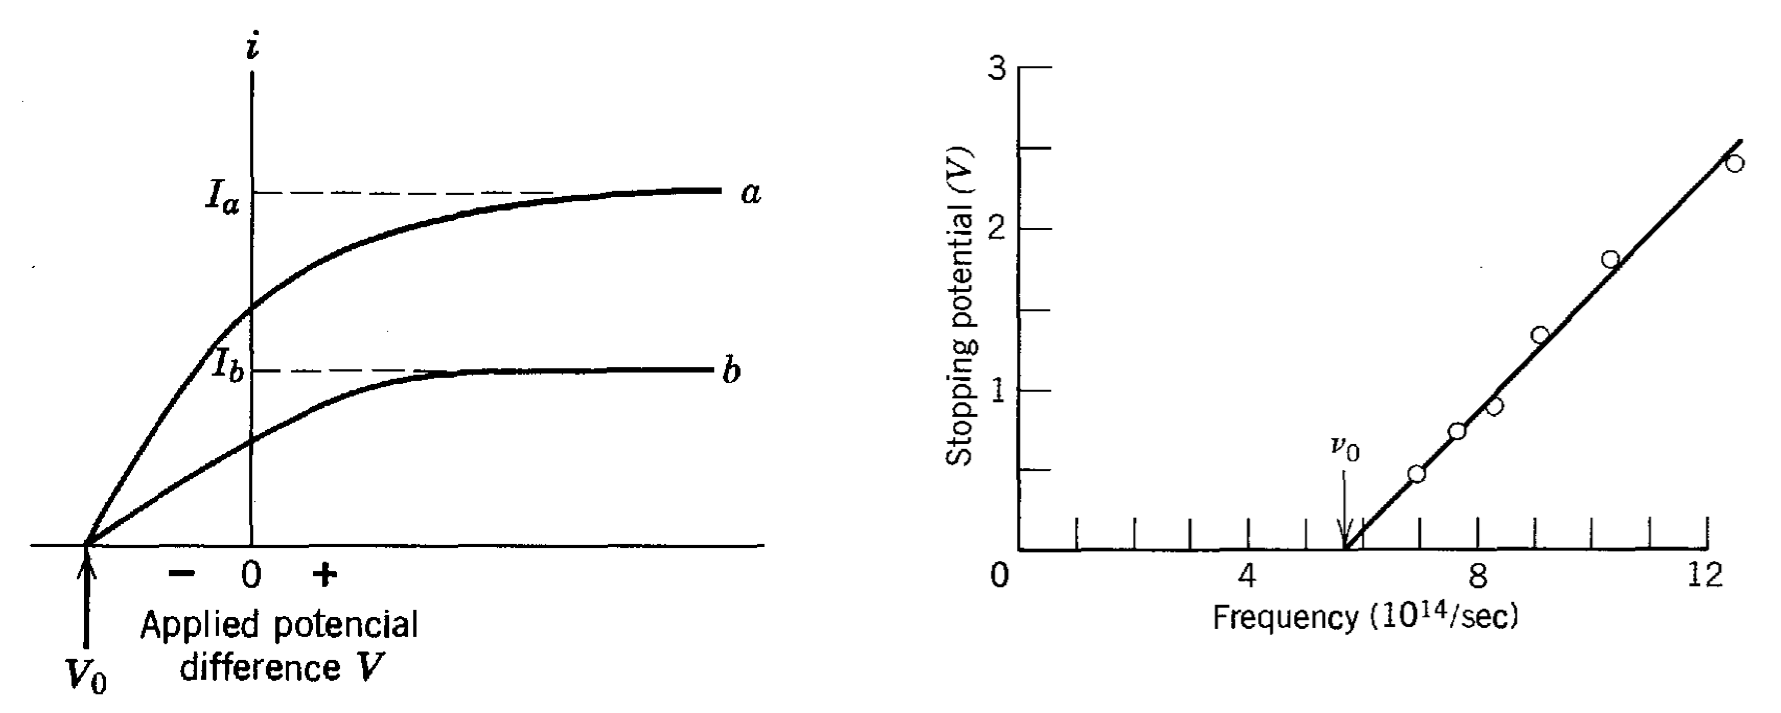
\includegraphics[scale=0.2]{/effetto_fotoelettrico}
\caption{Risultati esperimento}
\label{risultati_Lenard}
\end{figure}

L'energia cinetica massima dei fotoelettroni emessi dall'elettrodo è
\begin{equation}
K_{max} = e V_0
\end{equation}

Se considero una luce incidente con un'intensità massima $I_b$ (vedi grafico a sinistra in figura \ref{risultati_Lenard}), che si riferisce ad un'intensità minore rispetto a $I_a$, trovo un livello di saturazione minore rispetto al caso precedente ma vedo che il valore $V_0$ non cambia: l'energia cinetica massima degli elettroni non cambia, risulta essere indipendente dall'intensità della luce.

\underline{Il secondo risultato sperimentale} trovato (grazie al contributo di Millican, vedi grafico a destra in figura \ref{risultati_Lenard}) è che se grafico il potenziale di stop in funzione della frequenza della radiazione incidente trovo una relazione lineare, ma al di sotto di un certo valore di frequenza $\nu_0$ che prende il nome di \textit{frequenza di cutoff} non osservo più l'effetto fotoelettrico: ovvero non osservo più l'emissione di elettroni dall'elettrodo colpito dalla radiazione.




La fisica classica, con la teoria ondulatoria della luce, non è in grado di spiegare tre aspetti fondamentali di questo fenomeno:
\begin{enumerate}[label=\Roman{*}]
\item Poiché l'intensità della luce è proporzionale all'ampiezza del vettore campo elettrico al quadrato, il campo elettrico $\vec E$ dovrebbe aumentare all'aumentare dell'intensità della luce.
La forza applicata all'elettrone dovrebbe essere proporzionale al vettore campo elettrico e con esso l'energia cinetica degli elettroni dovrebbe aumentare, ma questo non accade: non si vede una dipendenza dell'energia cinetica dell'elettrone dall'intensità della luce incidente.

\item Esiste una frequenza di cutoff, e non si spiega il perché. Se la luce è abbastanza intensa e fornisce abbastanza energia l'effetto dovrebbe verificarsi per qualsiasi frequenza, per la teoria ondulatoria, ma non è così. 

\item Considerando una luce incidente molto debole, l'elettrone dovrebbe aver bisogno di un certo tempo per accumulare sufficiente energia per essere emesso, dovrebbe esserci un tempo misurabile in cui questo avviene.
Eppure non si misura nessun ritardo fra il momento in cui la luce incide sull'elettrodo e l'emissione dell'elettrone, l'esperimento sembra suggerire che il fenomeno avvenga istantaneamente.
\end{enumerate}

\subsection{Spiegazione dell'effetto fotoelettrico di Einstein}
La radiazione elettromagnetica è costituita da un'insieme di pacchetti di energia, che oggi chiamiamo \textit{fotoni} (denominati così da un chimico: Lewis), di energia data da
\begin{equation}
E = h \nu
\end{equation}
dove $h$ è la costante di Planck e $\nu$ è la frequenza della radiazione.

Che differenza c'è rispetto a Planck?
Planck aveva applicato la quantizzazione dell'energia agli elettroni accelerati sulle pareti di cavità, poi pensava che la radiazione si propagasse come onde di energia quantizzata, ma onde.
Einstein propone che l'energia che si irradia (scambiata tra pareti e onde nella cavità, se pensiamo al corpo nero) venga scambiata in pacchetti di quantità $h\nu$ che rimangono tali anche successivamente allo scambio.
Egli non contesta che la luce possa essere descritta in termini ondulatori, sottolinea la natura corpuscolare della radiazione in fenomeni in cui la radiazione viene emessa e assorbita.

\begin{equation}
\begin{split}
Planck \quad & \Rightarrow \quad \mbox{onde di energia quantizzata} \\
Einstein \quad & \Rightarrow \quad \mbox{pacchetti di energia quantizzata} 
\end{split}
\end{equation}

L'effetto fotoelettrico per Einstein consiste nel completo assorbimento di un fotone da parte di un elettrone del catodo, che viene appunto fotoemesso.
La spiegazione matematica è la seguente
\begin{equation}
K = h\nu - W
\end{equation}
dove l'energia cinetica dell'elettrone emesso $K$ equivale alla differenza fra l'energia del fotone $h\nu$ completamente assorbito e una quantità $W$ che è il lavoro richiesto per strappare l'elettrone dal metallo.
L'energia cinetica massima è descritta dalla legge di Einstein per l'effetto fotoelettrico
\begin{equation}
K_{max} = h\nu - W_0
\end{equation}
Dove $W_0$ prende il nome di \textit{funzione lavoro} ed è una caratteristica del metallo utilizzato e corrisponde all'energia minima dell'elettrone per uscire dal catodo.

Dalla formula di Einstein si ricava il potenziale di stop:
\begin{equation}
\begin{split}
& K_{max} = h\nu - W_0 \\
& V_0 = \frac{ h\nu}{e } - \frac{ W_0}{e }
\end{split}
\end{equation}
quindi permette di comprendere meglio la relazione lineare tra il potenziale  di stop e la frequenza, vista in figura \ref{risultati_Lenard}.
La pendenza di tale curva è $\frac{ h}{e }$ e l'intercetta all'asse delle ordinate è $\frac{ W_0}{e }$; da questo studio è anche possibile ricavare la costante di Planck, come fece Millican trovando un valore molto vicino a quello che oggi riteniamo esatto.

\newpage

Quindi Einstein ci mette nella condizione di poter rispondere ai quesiti posti in precedenza dalla fisica classica:
\begin{enumerate}[label=\Roman{*}]
\item "$K_{max}$ non dipende dall'intensità della luce" \\
Raddoppiare l'intensità della luce incidente, mantenendo la stessa frequenza, significa raddoppiare il numero di fotoni, ma il valore dell'energia di ogni fotone $h\nu$ rimane invariato e, appunto, $K_{max}$ non dipende dall'intensità della luce.

\item "Esistenza della frequenza di cutoff"\\
Se $K_{max} = 0 \quad \Rightarrow \quad h\nu_0 = W_0$ viene strappato un elettrone ma senza energia cinetica ed è quindi il limite per il verificarsi dell'effetto fotoelettrico, $\nu_0$ è la frequenza di cutoff.

\item "Non c'è un tempo di interazione"\\
L'energia è fornita in pacchetti concentrati di energia e quindi quando un fotone viene assorbito è assorbito tutto in una volta ed immediatamente si ha l'emissione di un elettrone.
\end{enumerate}

\textbf{NB:} l'effetto fotoelettrico, quindi un completo assorbimento del fotone incidente, può avvenire anche con fotoni di più alta energia del visibile (e.g. raggi X), che però andrà ad estrarre gli elettroni più legati al nucleo.

\subsection{Raffigurazione dello spettro elettromagnetico}
\begin{figure}[h]
\centering
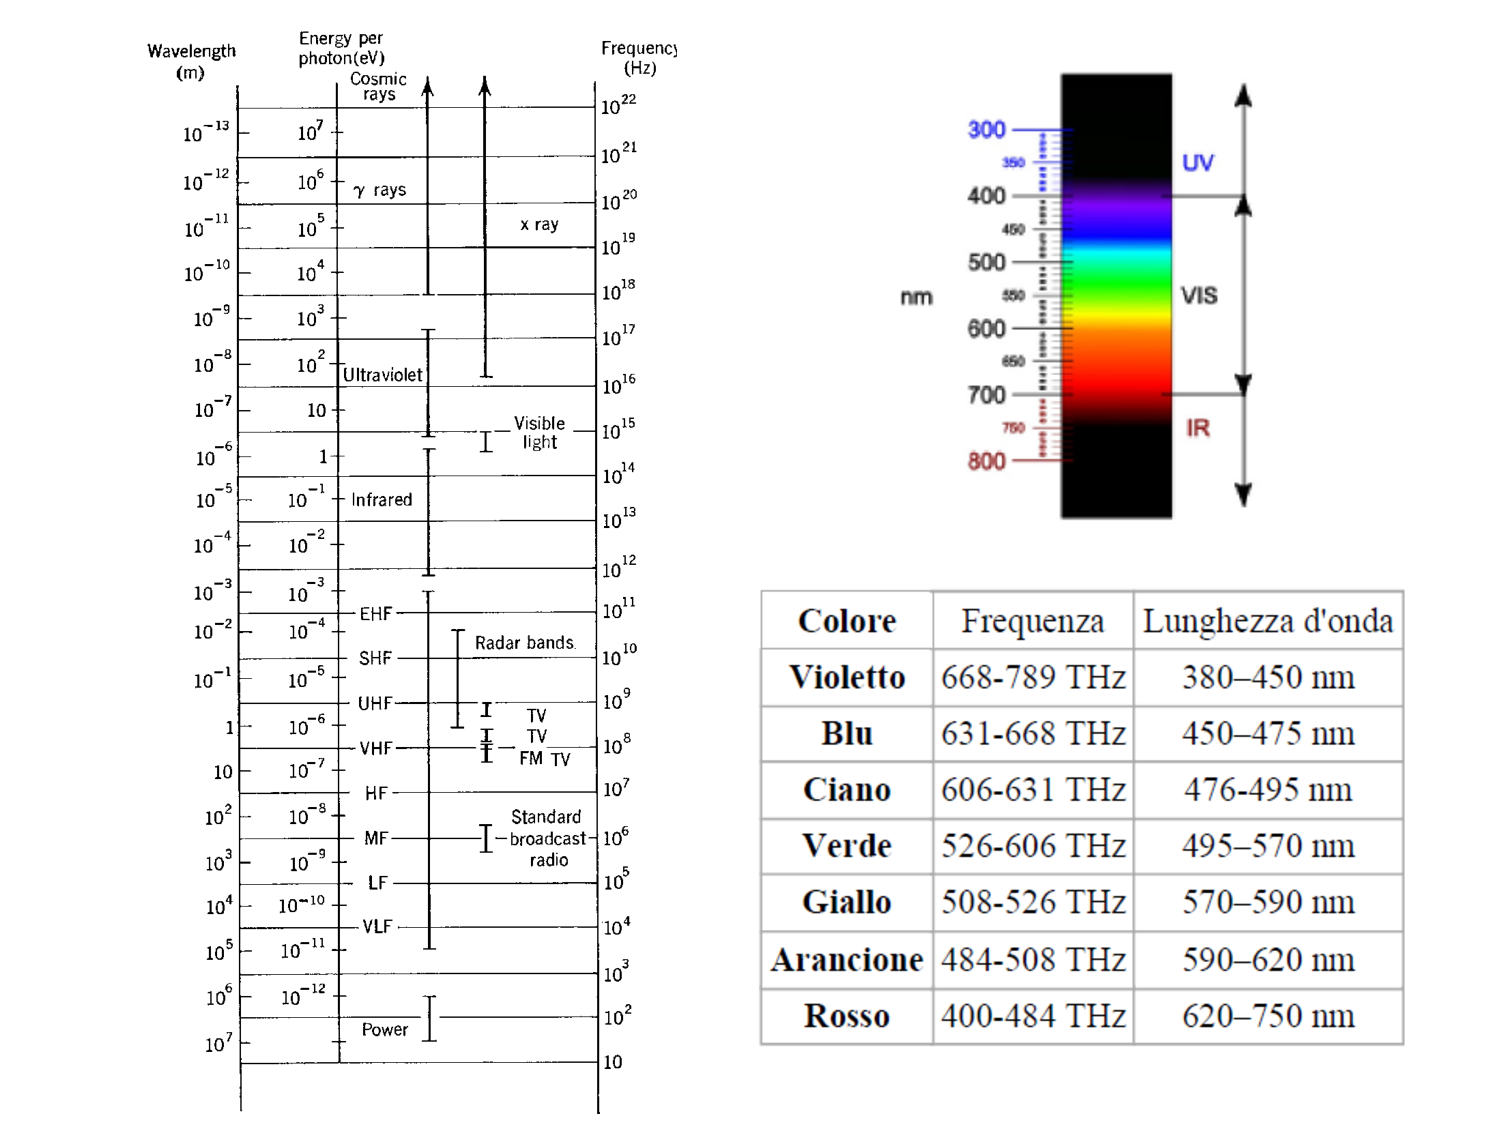
\includegraphics[scale=0.6]{/spettro_elettromagnetico}
\caption{Spettro elettromagnetico}
\end{figure}



    %%
%% Author: dariochinelli
%% 2021-03-11
%%

\section{Effetto Compton}

L'effetto Compton è, come l'effetto fotoelettrico, un fenomeno di interazione tra radiazione e materia, si tratta però di fotoni molto più energetici come i fotoni X.
È denominato scattering o diffusione poiché viene interpretato come un urto anelastico tra il fotone e l'elettrone per cui non vi è quindi assorbimento del fotone ed è questa la differenza fondamentale dall'effetto fotoelettrico.

\subsection{Esperimento di Compton}
\begin{figure}[h]
\centering
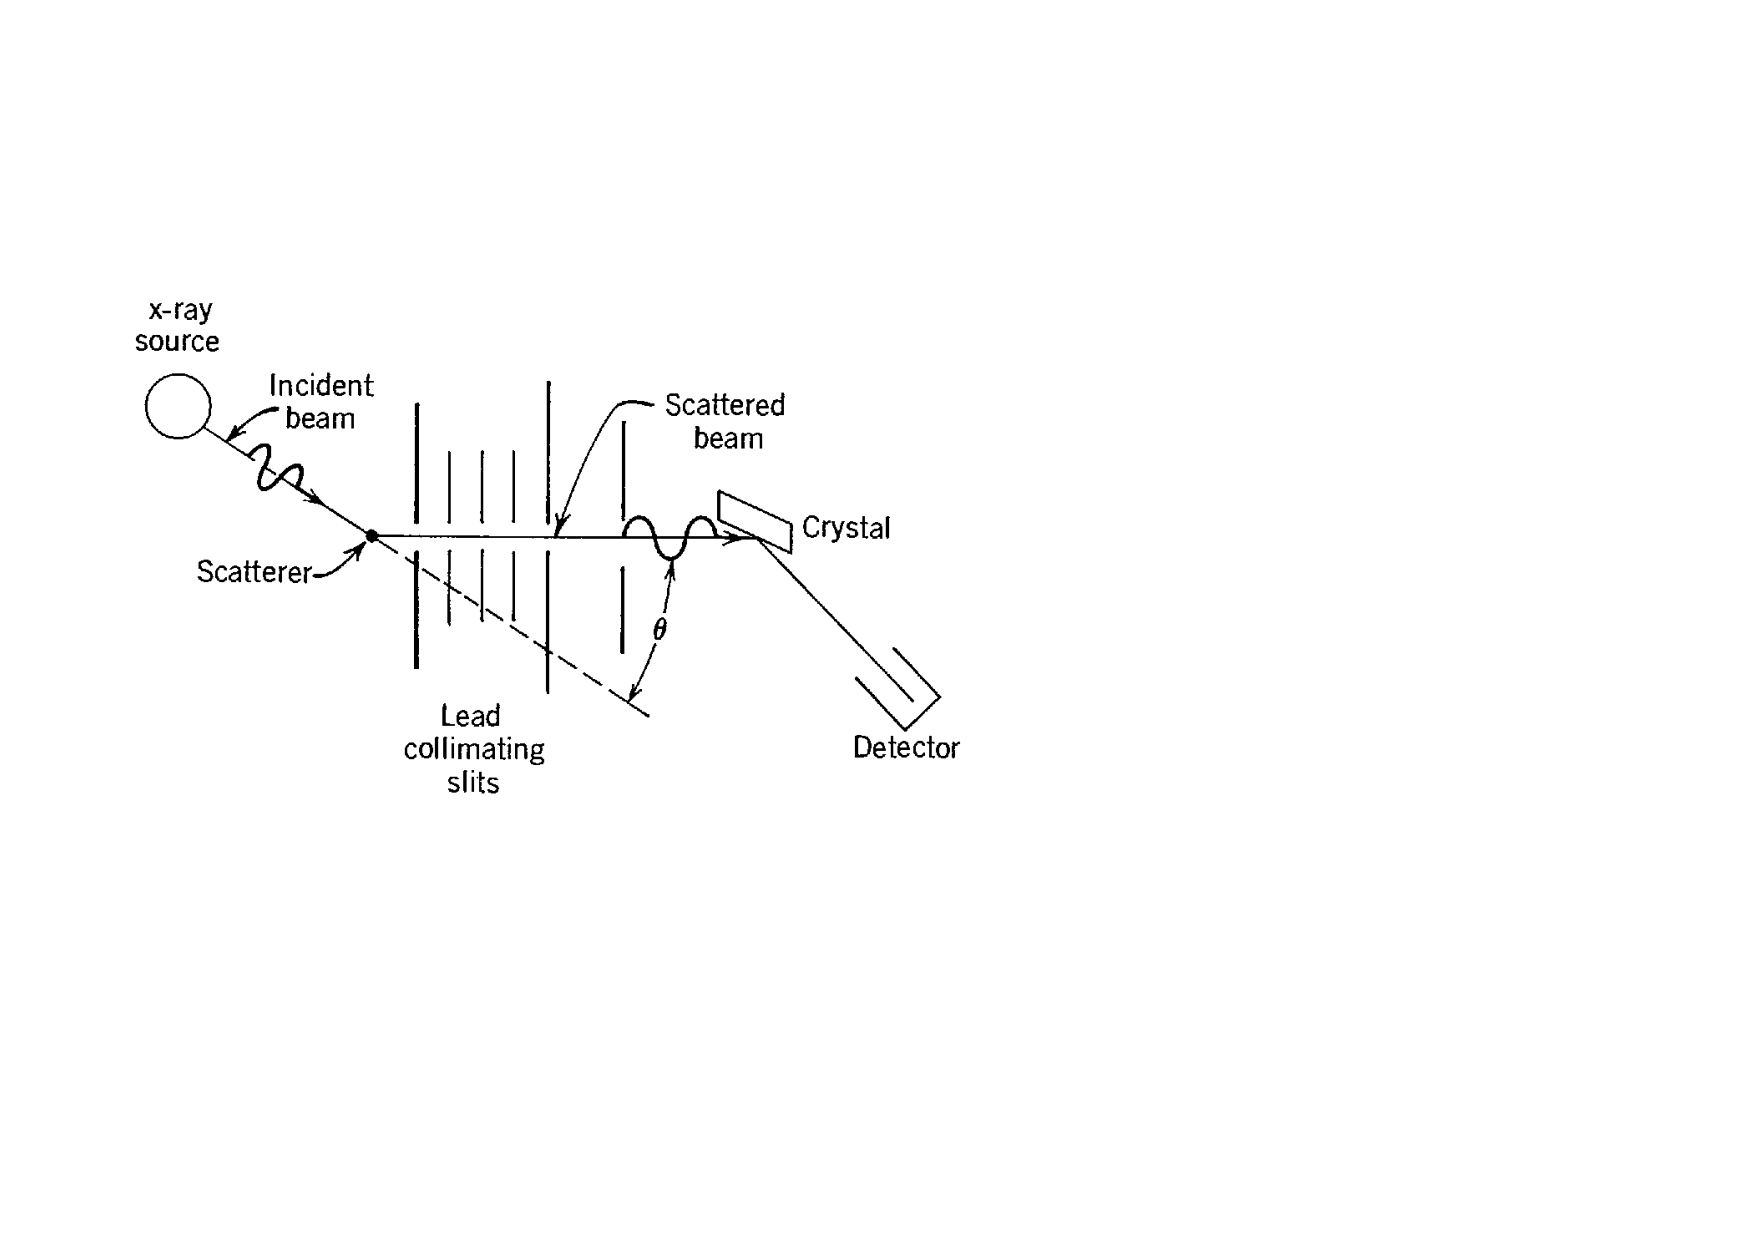
\includegraphics[scale=0.75]{/effettoCompton_setup}
\caption{Setup sperimentale dell'esperimento di Compton}
\end{figure}

Nell'esperimento del 1922, un fascio di fotoni X monocromatico, quindi una $\lambda = \SI{0.709}{\AA}$ molto precisa, viene fatto incidere su un target di carbonio, ed in seguito a questo viene diffusa radiazione X su tutto l'angolo solido.
Compton \textbf{misura l'intensità} della radiazione diffusa in funzione della lunghezza d'onda a diversi angoli di diffusione $\theta$.
Nell'apparato sperimentale vengono posti dei collimatori del fascio "slits" e l'apparato che consente di eseguire la misura: uno spettrometro di Bragg costituito da un cristallo e un detector, che vediamo in seguito.

Vediamo i risultati ottenuti da Compton in figura \ref{compton_results}.
Quando $\theta = 0$ si vede un picco di intensità, centrato sullo stesso valore di $\lambda$ del raggio incidente.
Se aumento l'angolo $\theta$ di fianco al primo picco ne compare un secondo ad una lunghezza d'onda maggiore rispetto al primo,
aumentando sempre di più l'angolo i due picchi si distinguono sempre meglio.
La presenza di questo secondo picco non è spiegabile con la fisica classica, solo il primo picco lo è.

\begin{figure}[h]
\centering
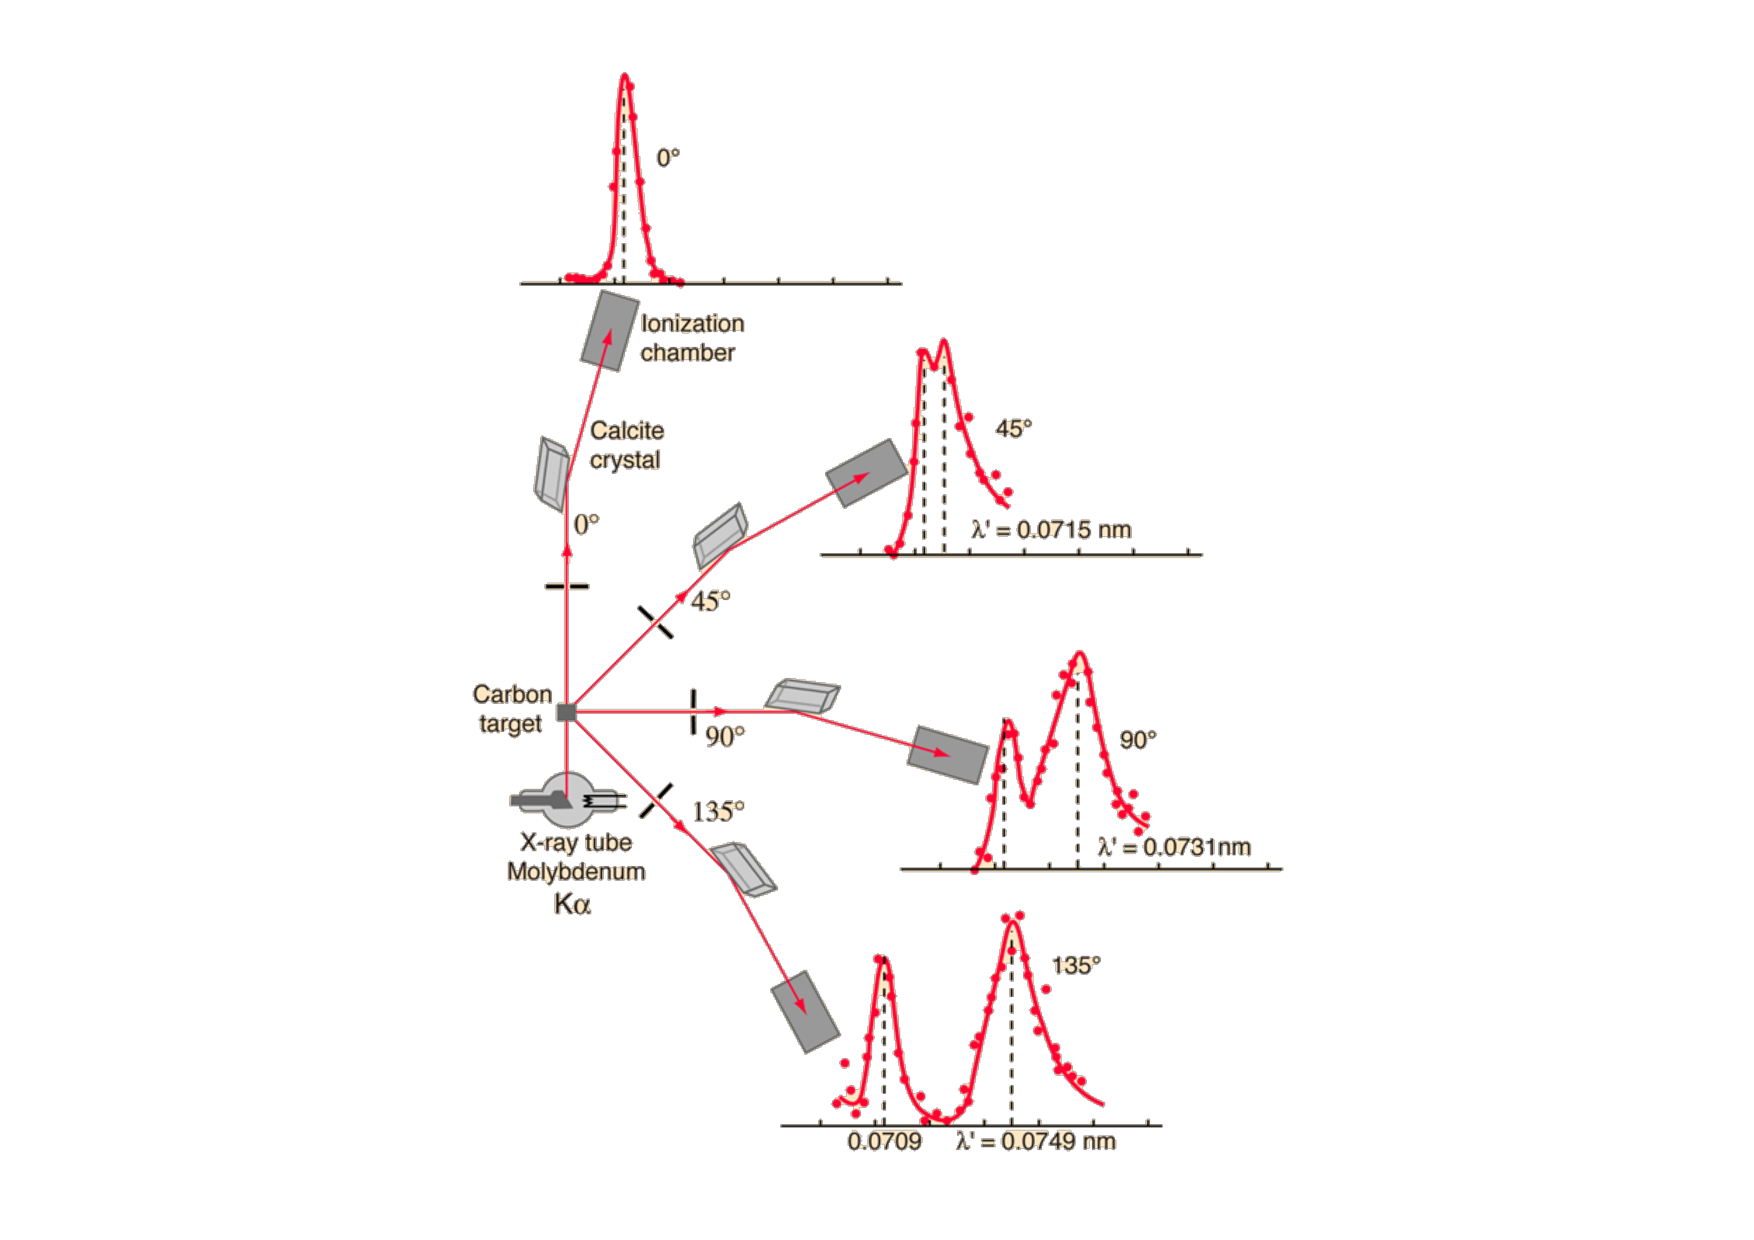
\includegraphics[scale=0.5]{/effettoCompton_risultati}
\caption{Risultati di Compton sulla misura dell'intensità della radiazione diffusa in funzione della lunghezza d'onda $\lambda$ a diversi angoli $\theta$}
\label{compton_results}
\end{figure}

\subsection{Spiegazione di Compton}

La spiegazione data da Compton (e Debye) è assumere che il fascio irraggiante X fosse composto da fotoni e che avvenisse un \textit{urto} tra un fotone e un elettrone \textit{libero} all'interno del target.
Quindi l'energia del fotone incidente $E$ iniziale verrà trasferita in parte all'elettrone, in seguito a ciò il fotone avrà energia finale minore e quindi lunghezza d'onda maggiore.
Nell'effetto Compton i fotoni non sono quindi assorbiti ma \textit{scatterati} e tali fotoni costituiranno il secondo picco rilevato nell'esperimento.
Definisco l'elettrone come \textit{libero} poiché il rapporto tra l'energia del fotone incidente e quella di estrazione dell'elettrone è molto grande, di conseguenza posso applicare alcune approssimazioni.

\begin{equation}
\begin{split}
E = \frac{ m_0 c^2}{\sqrt{1 - \frac{ v^2}{c^2 }} } & \quad \mbox{energia di una particella relativistica con massa} \\
E = h \nu & \quad \mbox{energia del fotone, che ha massa nulla} \\ \\
E^2 = c^2 p^2 + (m_0 c^2)^2 & \quad \mbox{per il fotone il secondo termine è zero} \\
p = \frac{ E}{c } = \frac{ h \nu}{c } = \frac{ h}{ \lambda} & \quad \mbox{quantità di moto del fotone} \quad \mbox{dove uso} \quad \lambda \nu = c
\end{split}
\end{equation}

Studiamo il processo di interazione uguagliando il momento totale prima e dopo l'interazione e l'energia totale prima e dopo la collisione.
Indico con $E_0, p_0$ l'energia e il momento del fotone incidente e con $\lambda$ la sua lunghezza d'onda, considero l'elettone inizialmente fermo.
Dopo la collisione indico con $E_1, p_1$ l'energia e il momento del fotone diffuso e con $\lambda'$ la sua lunghezza d'onda; 
indico con $K, p$ l'energia ed il momento dell'elettrone dopo l'urto;
indico inoltre con $\theta$ l'angolo di diffusione del fotone e con $\phi$ l'angolo di diffusione dell'elettrone.
Considerare inoltre che, al contrario del fotone, l'elettrone ha massa e quindi energia a riposo non nulla pari a $m_{0,e}c^2$.

\begin{figure}[h]
\centering
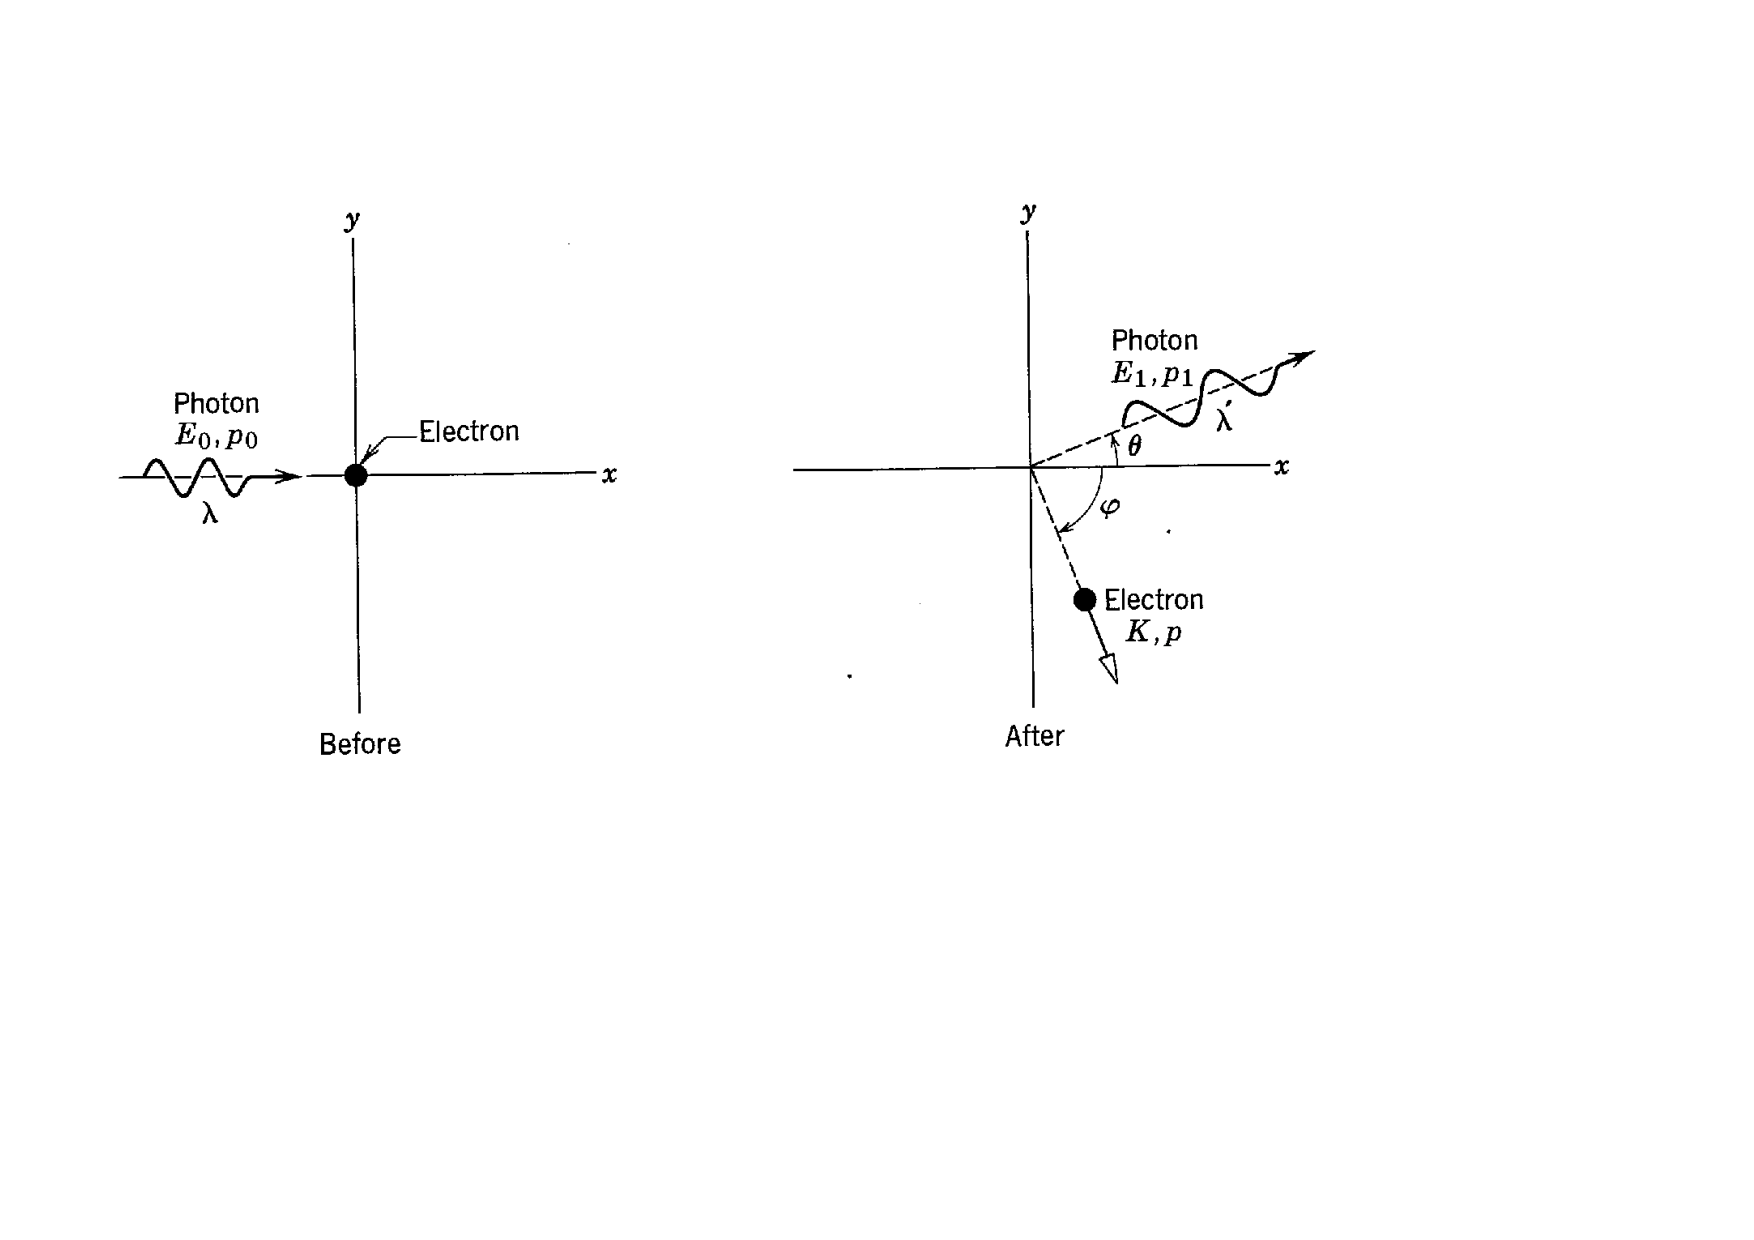
\includegraphics[scale=0.6]{/effettoCompton_schema_interazione}
\caption{ Effetto Compton. Un fotone di lunghezza d'onda $\lambda$ incide su un elettrone a riposo. 
Nella collisione il fotone è scatterato di un angolo $\theta$ con lunghezza d'onda maggiore $\lambda '$, 
mentre l'elettrone si allontana con angolo $\varphi$ }
\end{figure}

Applichiamo la conservazione del momento angolare
\begin{equation}
\begin{split}
\mbox{lungo x} \quad & p_0 = p_1 \cos\theta + p \cos\varphi \\
\mbox{lungo y} \quad & p_1 \sin\theta = p \sin\varphi \\ \\
& (p_0 - p_1 \cos\theta)^2 = p^2 \cos^2\varphi \\
& p_1^2 \sin^2\theta = p^2 \sin^2\varphi \\ \\
\mbox{ottengo} \quad & p_0^2 + p_1^2 = 2 p_0 p_1 \cos\theta = p^2
\end{split}
\end{equation}

Applichiamo la conservazione dell'energia
\begin{equation}
\begin{split}
& E_0 + m_{0,e} c^2 = E_1 + K + m_{0,e} c^2 \\
& E_0 - E_1 = K \\ \\
\mbox{utilizzando} \quad & p =\frac{ E}{c } \\
\mbox{ottengo} \quad & c (p_0 - p_1) = K 
\end{split}
\end{equation}

Dalla relazione di mass shell relativistica applicata all'elettrone ottengo
\begin{equation}
\begin{split}
& E^2 = c^2 p^2 + (m_{0,e} c^2)^2 \\
& (K + m_{0,e} c^2)^2 = c^2 p^2 + (m_{0,e} c^2)^2 \\
& K^2 + 2 K m_{0,e} c^2 = c^2 p^2 \\
& \frac{ K^2}{c^2 } + 2Km_{0,e} = p^2
\end{split}
\end{equation}

In quest'ultima relazione sostituisco ora $p$ e $K$ dai risultati ottenuti in precedenza e trovo
\begin{equation}
\begin{split}
& (p_0 - p_1)^2 + 2m_{0,e} c (p_0 - p_1) = p_0^2 + p_1^2 - 2p_0 p_1 \cos\theta \\
& m_{0,e} c (p_0 - p_1) = p_0 p_1 (1 - \cos\theta) \\ \\
& \frac{ 1}{p_0 } - \frac{ 1}{p_1 } = \frac{ 1}{m_{0,e} c } (1 - \cos\theta)
\end{split}
\end{equation}

Moltiplicando per la costante di Planck $h$ ed utilizzando la formula $c = \lambda \nu$ si ottiene
\begin{equation}
\begin{split}
& \Delta \lambda = \lambda' - \lambda = \lambda_c (1 - \cos \theta) \\
& \lambda_c = \frac{ h}{m_{0,e} c } = \SI{2.43e-12}{m} = \SI{0.0000243}{nm} = \SI{2.43}{pm} = \SI{0.0243}{\AA}
\end{split}
\end{equation}
$\Delta \lambda$ definisce la distanza tra i due picchi visti nel grafico dei risultati dell'esperimento di Compton, inoltre la costante $\lambda_c$ è detta \textit{lunghezza d'onda di Compton}. \\
Quindi lo shift di Compton dipende \underline{solo} da $\theta$, per cui il valore minimo $\Delta \lambda = 0$ si ha per $\theta = 0$ ed il valore massimo $\Delta \lambda = \frac{ 2 h }{m_{0,e} c }$ per $\theta = \pi$.

\begin{figure}[h]
\centering
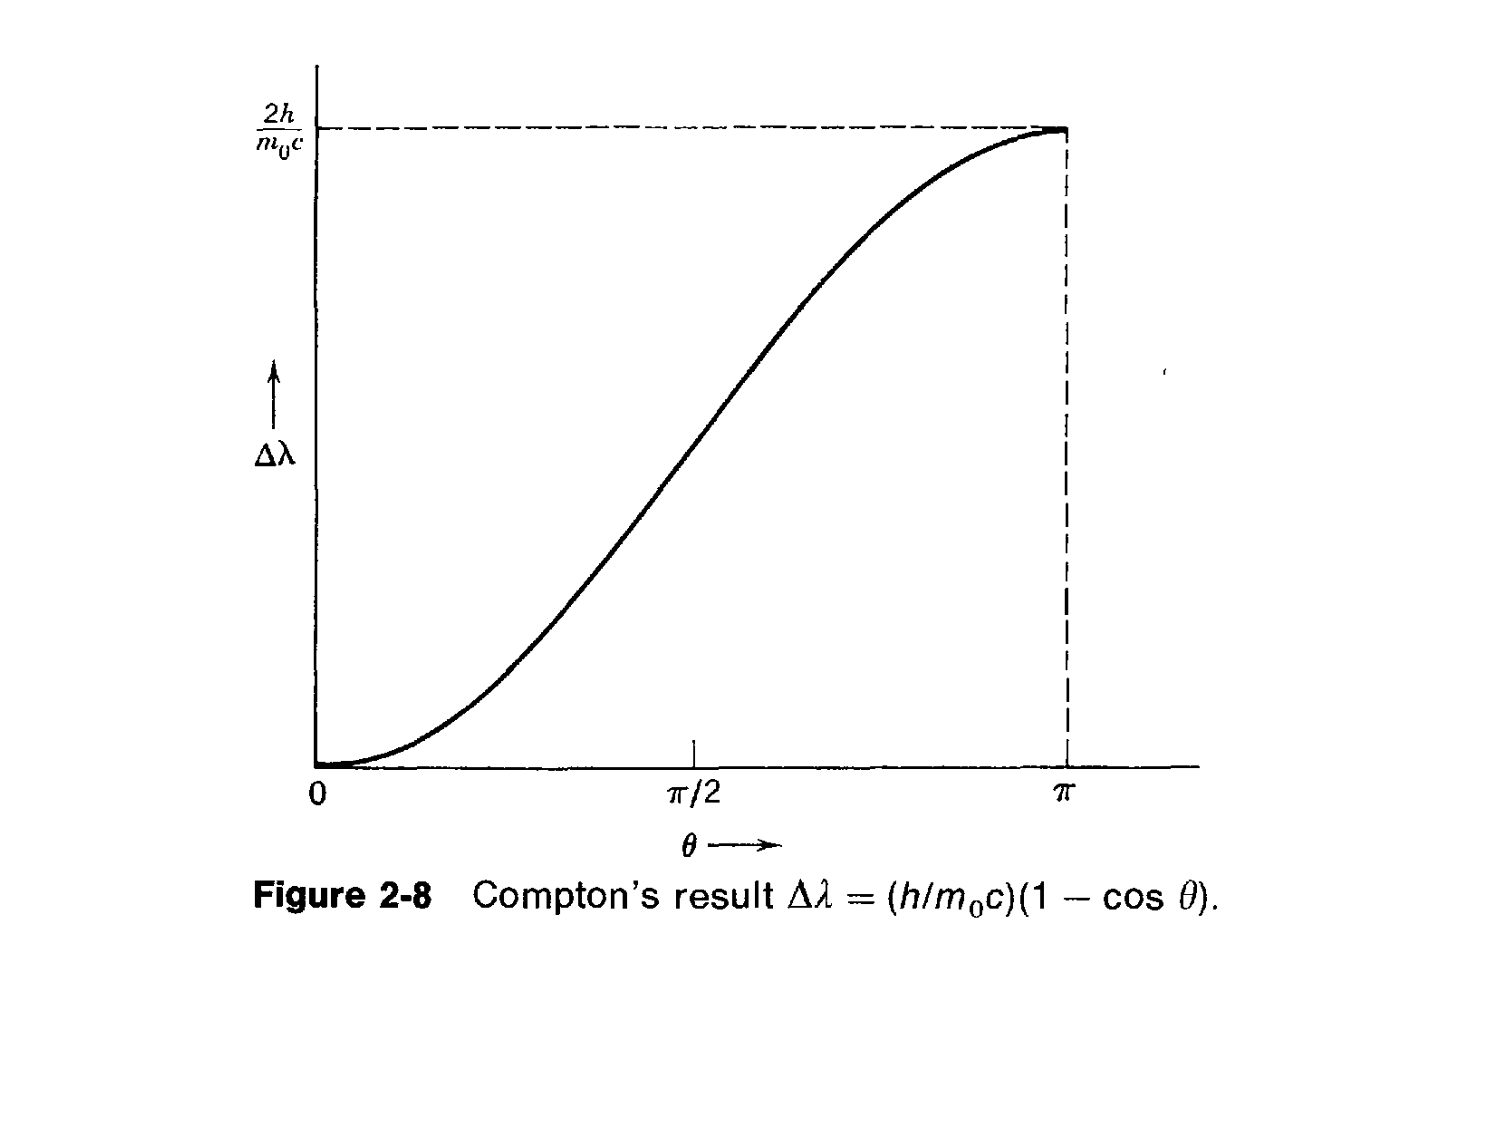
\includegraphics[scale=0.5]{/compton_deltalambda}
\caption{Andamento di $\Delta\lambda$ in funzione dell'angolo $\theta$}
\end{figure}

\textbf{NB:} Nell'esperimento di Compton ho due processi di interazione fra radiazione e materia: alcuni fotoni sono diffusi da elettroni che considero liberi e che vengono poi espulsi dal materiale, altri fotoni vengono diffusi da elettroni che rimangono legati al nucleo per cui non vi è una variazione della lunghezza d'onda dei fotoni, questo secondo processo prende il nome di scattering di Rayleigh (o scattering di Thompson).
Se la radiazione incidente fosse nel visibile o nelle onde radio, la lunghezza d'onda sarebbe talmente grande rispetto allo shift che non si potrebbe osservare tale fenomeno.



    %%
%% Author: dariochinelli
%% 2021-03-15
%%


\section{Diffrazione raggi X}
Nel 1913 Bragg scoprì che i solidi cristallini producevano pattern molto particolari nella diffrazione di raggi $X$.
Scoprì infatti che questi cristalli, a determinate lunghezze d'onda, producono picchi di intensità di radiazione diffusa ad angoli ben precisi.

\begin{figure}[h]
\centering
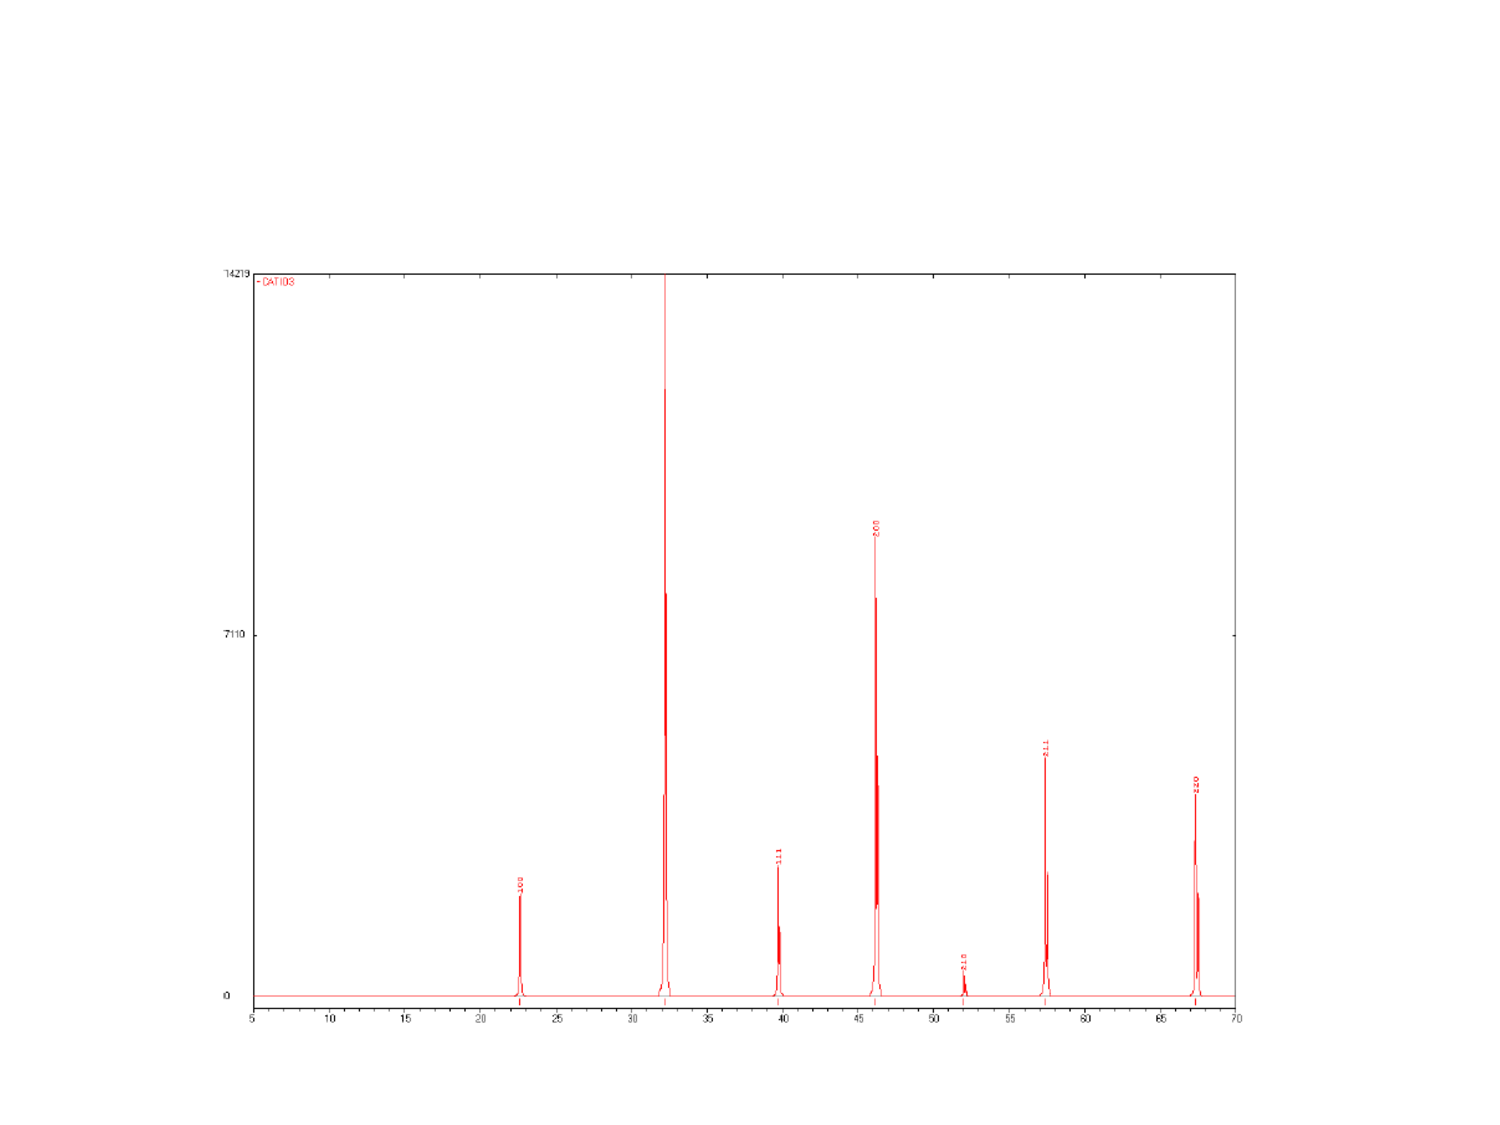
\includegraphics[scale=0.5]{/diffusione_raggiX}
\caption{Picchi di intensità per un materiale cristallino con struttura cubica}
\end{figure}

Cos'è un \textit{reticolo cristallino}? 
Si consideri ad esempio un pezzo di ferro, o alluminio, esso possiede un \textit{ordine cristallino}, ovvero gli atomi che lo compongono sono localizzati nello spazio in una struttura ordinata.
È come avere una matrice di atomi, posti in posizioni ben precise e ripetute "infinitamente" che compongono il materiale.
Per semplicità, consideriamo celle di forma cubica.

Per angoli ben precisi vedo quindi picchi della radiazione X, ciò è dovuto all'interferenza costruttiva che si ottiene dalla differenza di cammino ottico fra i due raggi riflessi da due atomi della struttura cristallina.
Venne spiegato da Max Von Laue.
\begin{figure}[h]
\centering
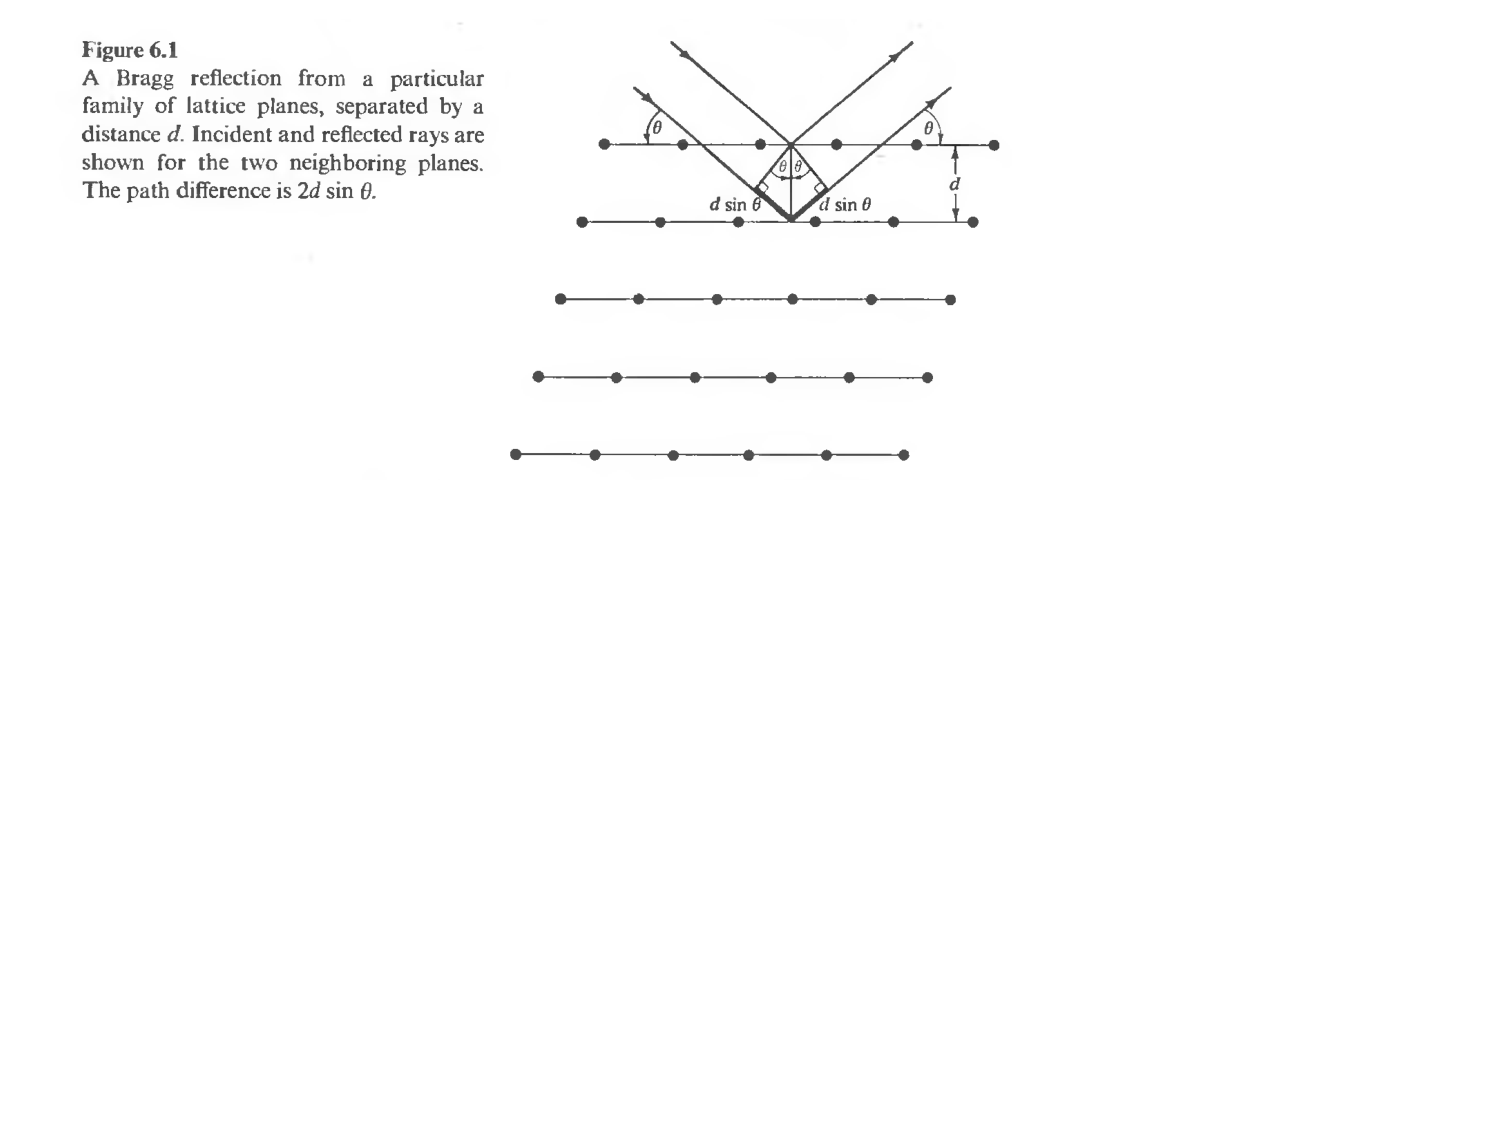
\includegraphics[scale=0.7]{/atomi_radiazineX}
\caption{Diagramma esplicativo della situazione}
\end{figure}

Pensando ad un reticolo di diffrazione: ogni fenditura è sorgente di onde;
Allo stesso modo ogni atomo si comporta come una sorgente d'onde e si verifica l'interferenza costruttiva.

Il contributo fondamentale per capire il fenomeno fu dato da William Henry Bragg e da William Lawrence Bragg, padre e figlio, i quali conoscendo i lavori di Von Laue capirono che si poteva spiegare il fenomeno assumendo che: \\ 
\textit{"per ogni raggio diffratto esiste un set di piani reticolari cosicché il raggio diffratto appare come riflesso specularmente da tale set di piani"}.
L'ipotesi di Bragg è che i piani siano semi-riflettenti.
\begin{figure}[h]
\centering
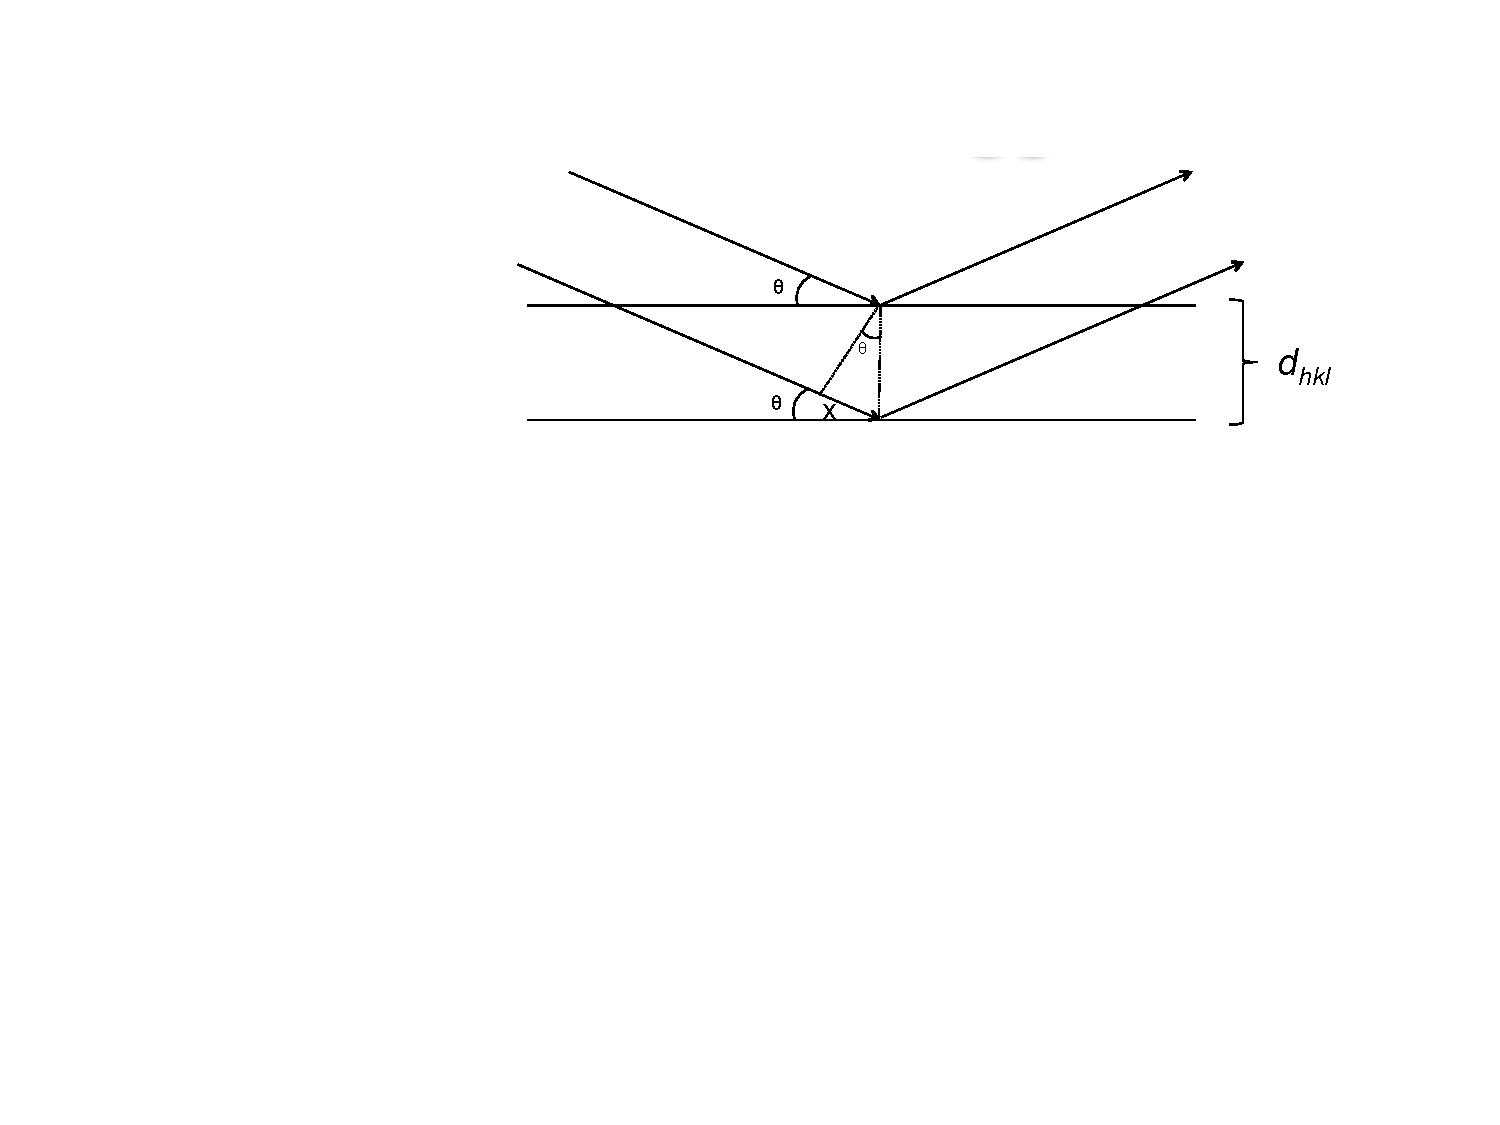
\includegraphics[scale=0.7]{/schema_bragg}
\caption{Schema cammini ottici}
\label{cammino_ottico}
\end{figure}

Come si vede in figura \ref{cammino_ottico} la differenza di cammino ottico sarà data da
\begin{equation}
\begin{split}
& \Delta = 2 (d \sin\theta) \\ 
& 2 d \sin\theta = n \lambda 
\end{split}
\end{equation}

Dove l'ultima equazione è la parte analitica della \textbf{Legge di Bragg}.

Bragg interpreta il fenomeno come una riflessione e non come una diffrazione, quando è verificata la condizione precedente.
Significa quindi che si tratta di picchi di \textit{riflessione} detti "picchi di riflessione di Bragg".
Per ogni tipo di cristallo potrò osservare tanti picchi di diffrazione ad angoli diversi, che corrispondono ad una riflessione da un set reticolare diverso.

Questo fenomeno è utile per investigare la materia:
sottoponendo un campione ad un fascio di raggi X risalgo alla sua struttura cristallina attraverso l'osservazione del pattern di diffrazione ottenuto.

\begin{figure}[h]
\centering
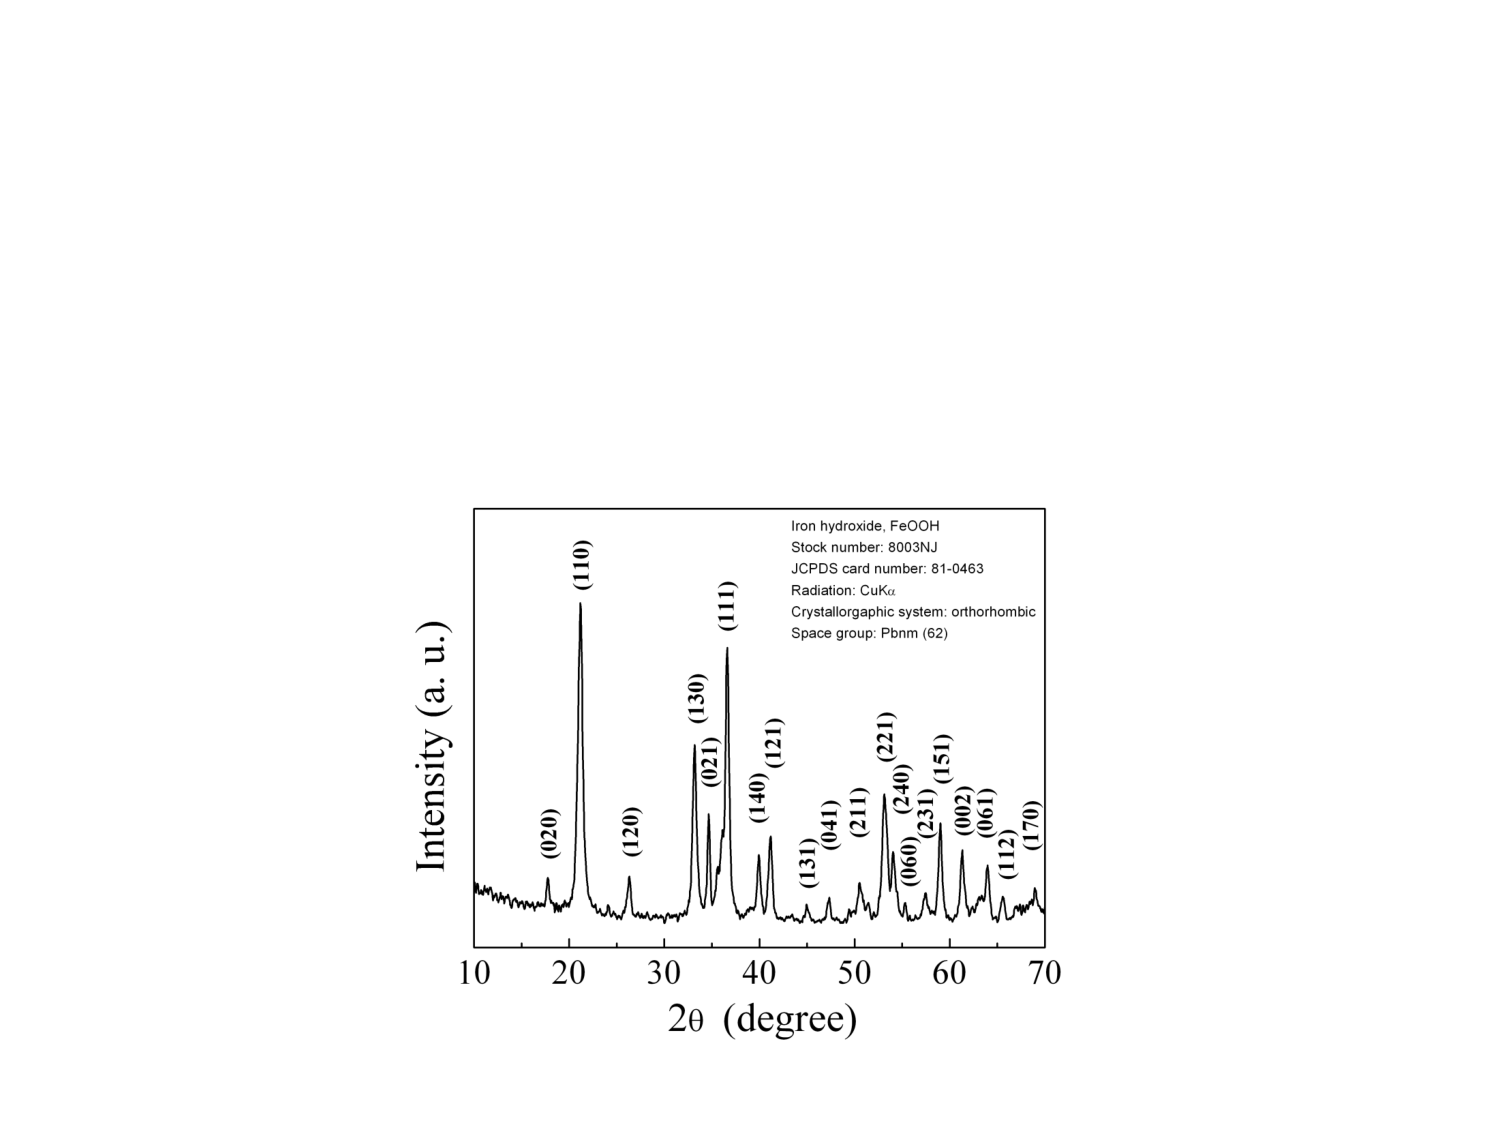
\includegraphics[scale=0.8]{/pattern_diffrazione_X}
\caption{Esempio di spettro di diffrazione}
\end{figure}



    %%
%% Author: dariochinelli
%% 2021-03-15
%%
\section{Fenomeni spiegabili solo con l'esistenza dei fotoni}

\subsection{Produzione raggi X}

La produzione di raggi X è un fenomeno di interazione tra radiazione e materia, è una prova della doppia natura delle onde elettromagnetiche.
I raggi X di questo tipo vengono prodotti da un \underline{tubo a raggi X} in cui ho un fascio di elettroni accelerati mediante una differenza di potenziale di migliaia di Volt (ordine $10^5$V), precedentemente liberati per \textit{effetto termoionico} da un filamento di Tungsteno riscaldato.
Gli elettroni incidono sull'anodo che li ferma con una decelerazione molto repentina che porta all'emissione di uno spettro continuo di radiazione elettromagnetica.

\begin{figure}[h]
\centering
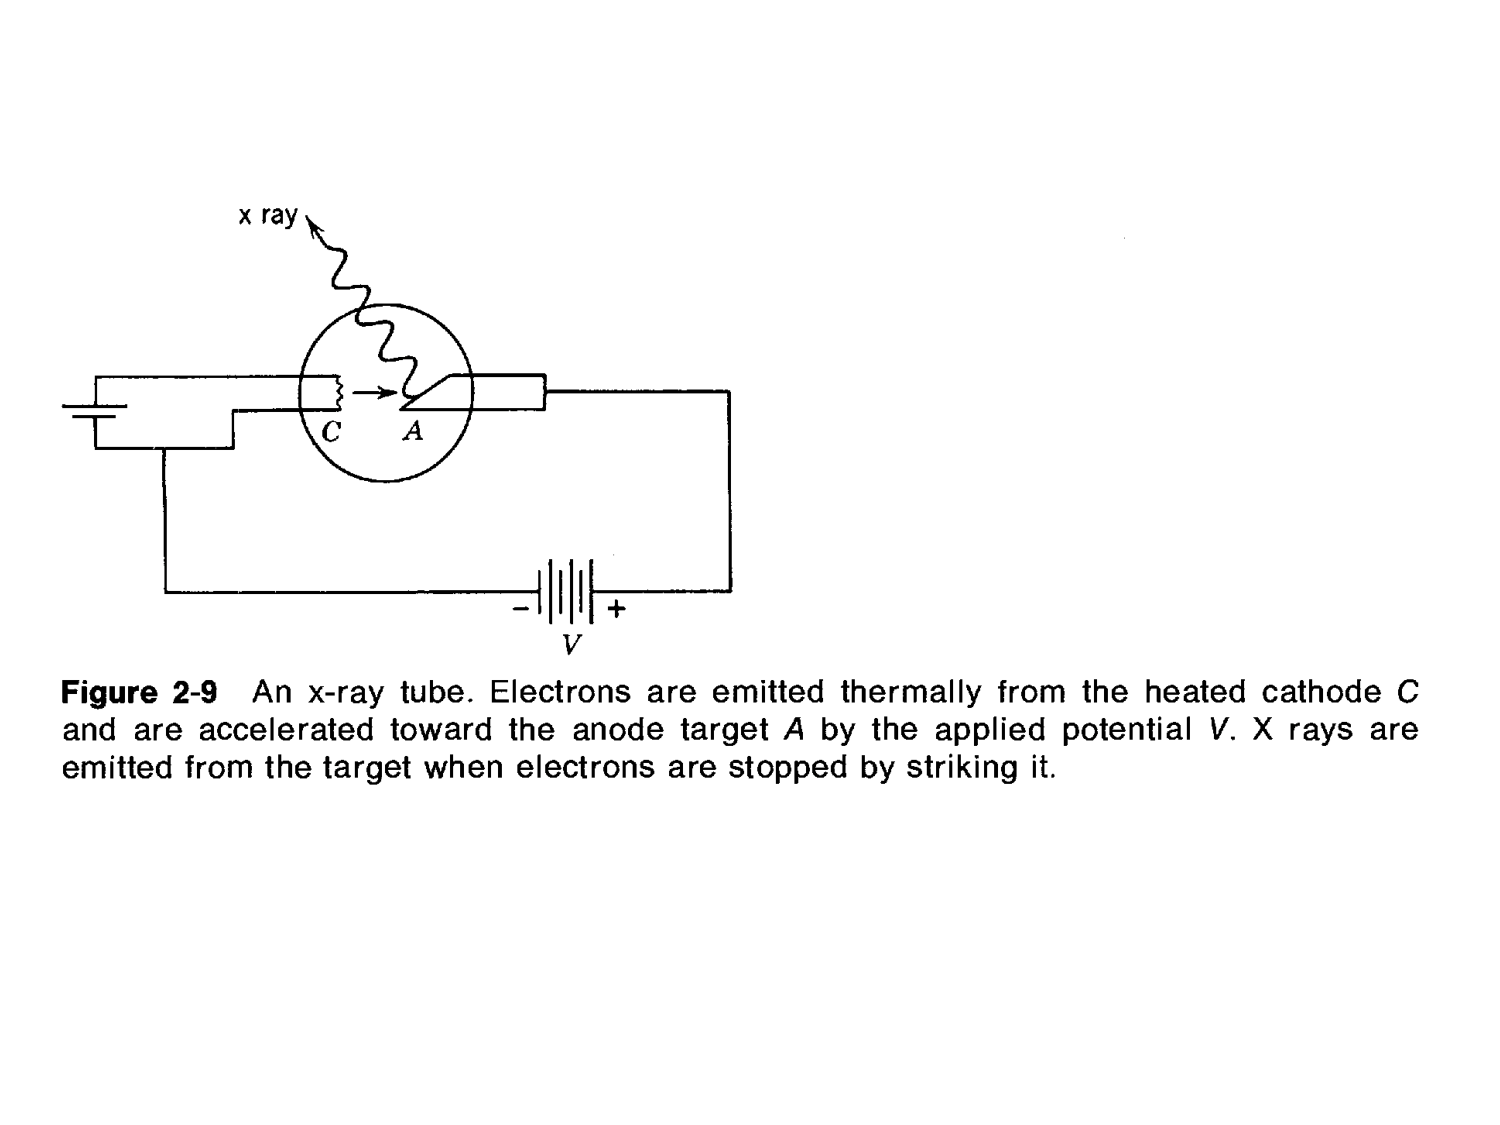
\includegraphics[scale=0.5]{/tubo_raggi_X}
\caption{Schema tecnico di produzione di raggi X}
\end{figure}

La $\lambda$ minima di emissione dipende solamente dall'energia applicata e non dal materiale di cui è costituito l'anodo.
\begin{figure}[h]
\centering
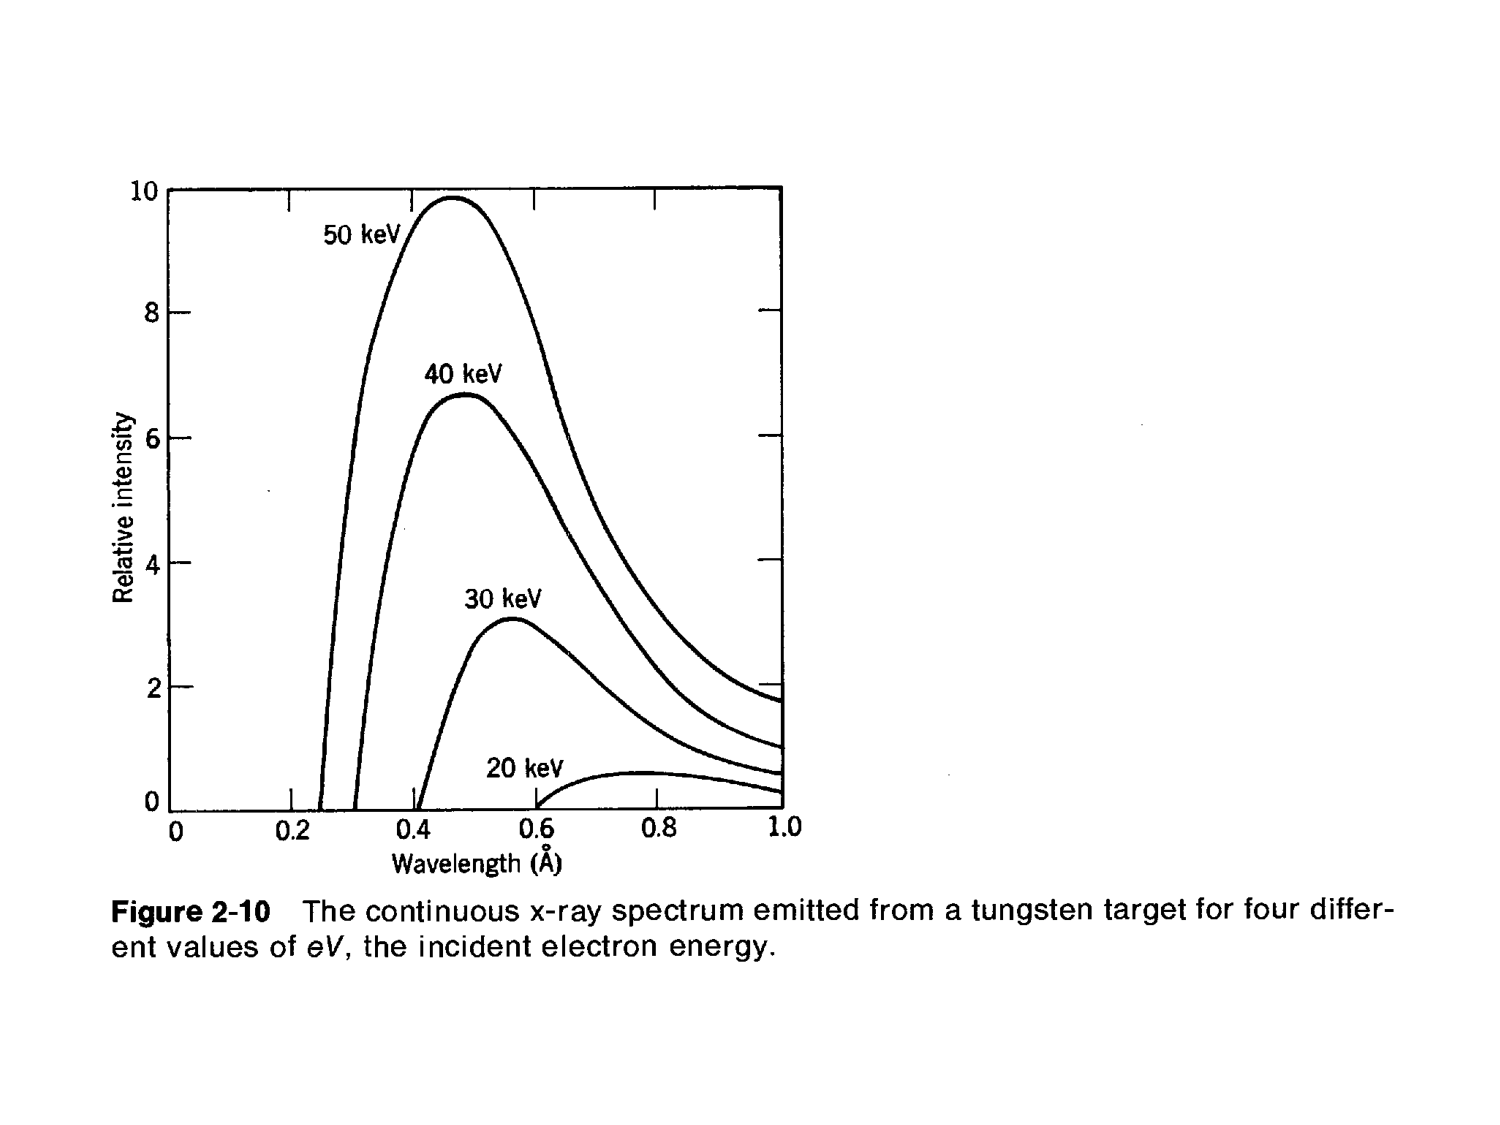
\includegraphics[scale=0.5]{/emissione_produzione_X}
\caption{Emissione che dipende solo dall'energia applicata nella differenza di potenziale}
\end{figure}

Questo fenomeno si spiega solo interpretando l'emissione come fotoni, fotoni X.
Un elettrone si fermerà dopo diverse interazioni di questo tipo, con una produzione continua di fotoni con diverse lunghezze d'onda,
variabile tra una $\lambda_{min}$ e infinito.
\begin{figure}[h]
\centering
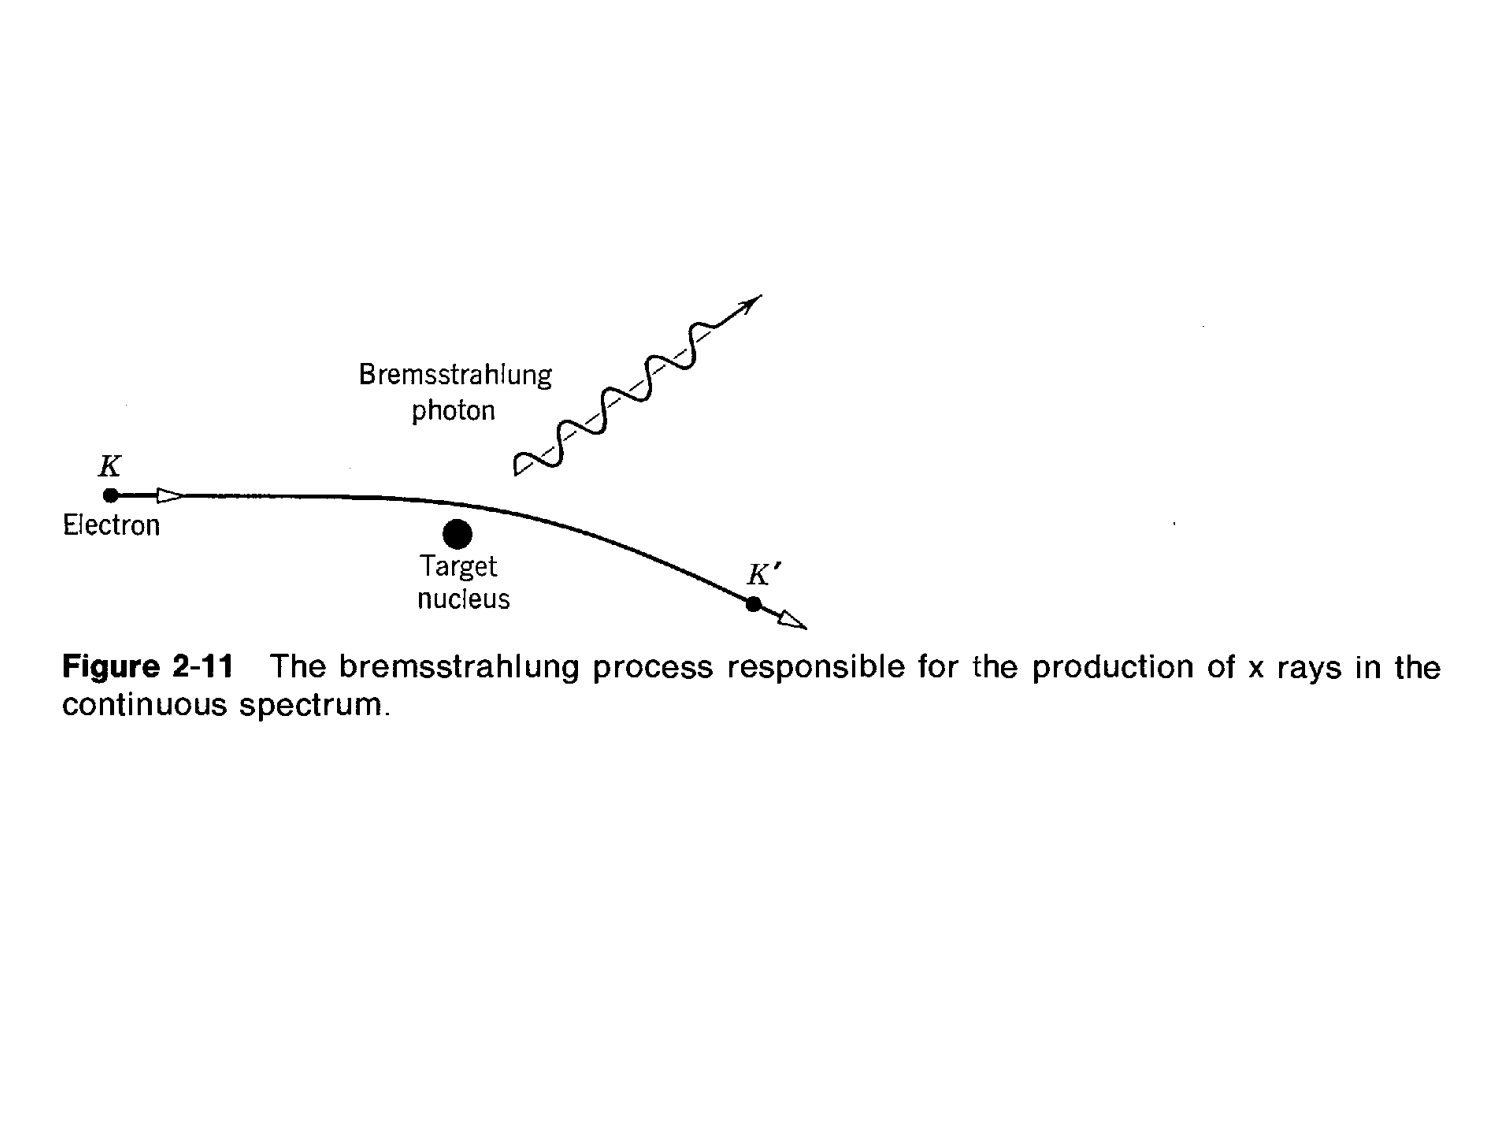
\includegraphics[scale=0.5]{/bremsstrahlung}
\caption{Schema interazione radiazione materia}
\end{figure}

\begin{equation}
\begin{split}
& h\nu = K - K' \\
& h \frac{ c}{\lambda } = K - K'
\end{split}
\end{equation}
Quando un elettrone perde tutta l'energia dopo un singolo evento ottengo la $\lambda$ minima:
\begin{equation}
\begin{split}
K' = 0 \quad & \Rightarrow \quad K = \frac{ hc}{\lambda_{min} } \\
eV = \frac{ hc}{\lambda_{min} } \quad & \Rightarrow \quad \lambda_{min} = \frac{ hc}{eV }
\end{split}
\end{equation}

Osservo che se la costante di Planck fosse nulla, la $\lambda_{min}$ tenderebbe a zero, ma così non è.
Questa radiazione elettromagnetica X è detta \textit{radiazione X di Bremsstrahlung}.

Si può vedere come l'inverso dell'effetto fotoelettrico!


\subsection{Produzione di coppie}

La produzione di coppie si verifica quando un fotone perde energia nell'interazione con un nucleo e si forma una coppia formata da un elettrone di energia $K_-$ e un positrone (particella analoga all'elettrone con carica positiva) di energia $K_+$.

\begin{figure}[h]
\centering
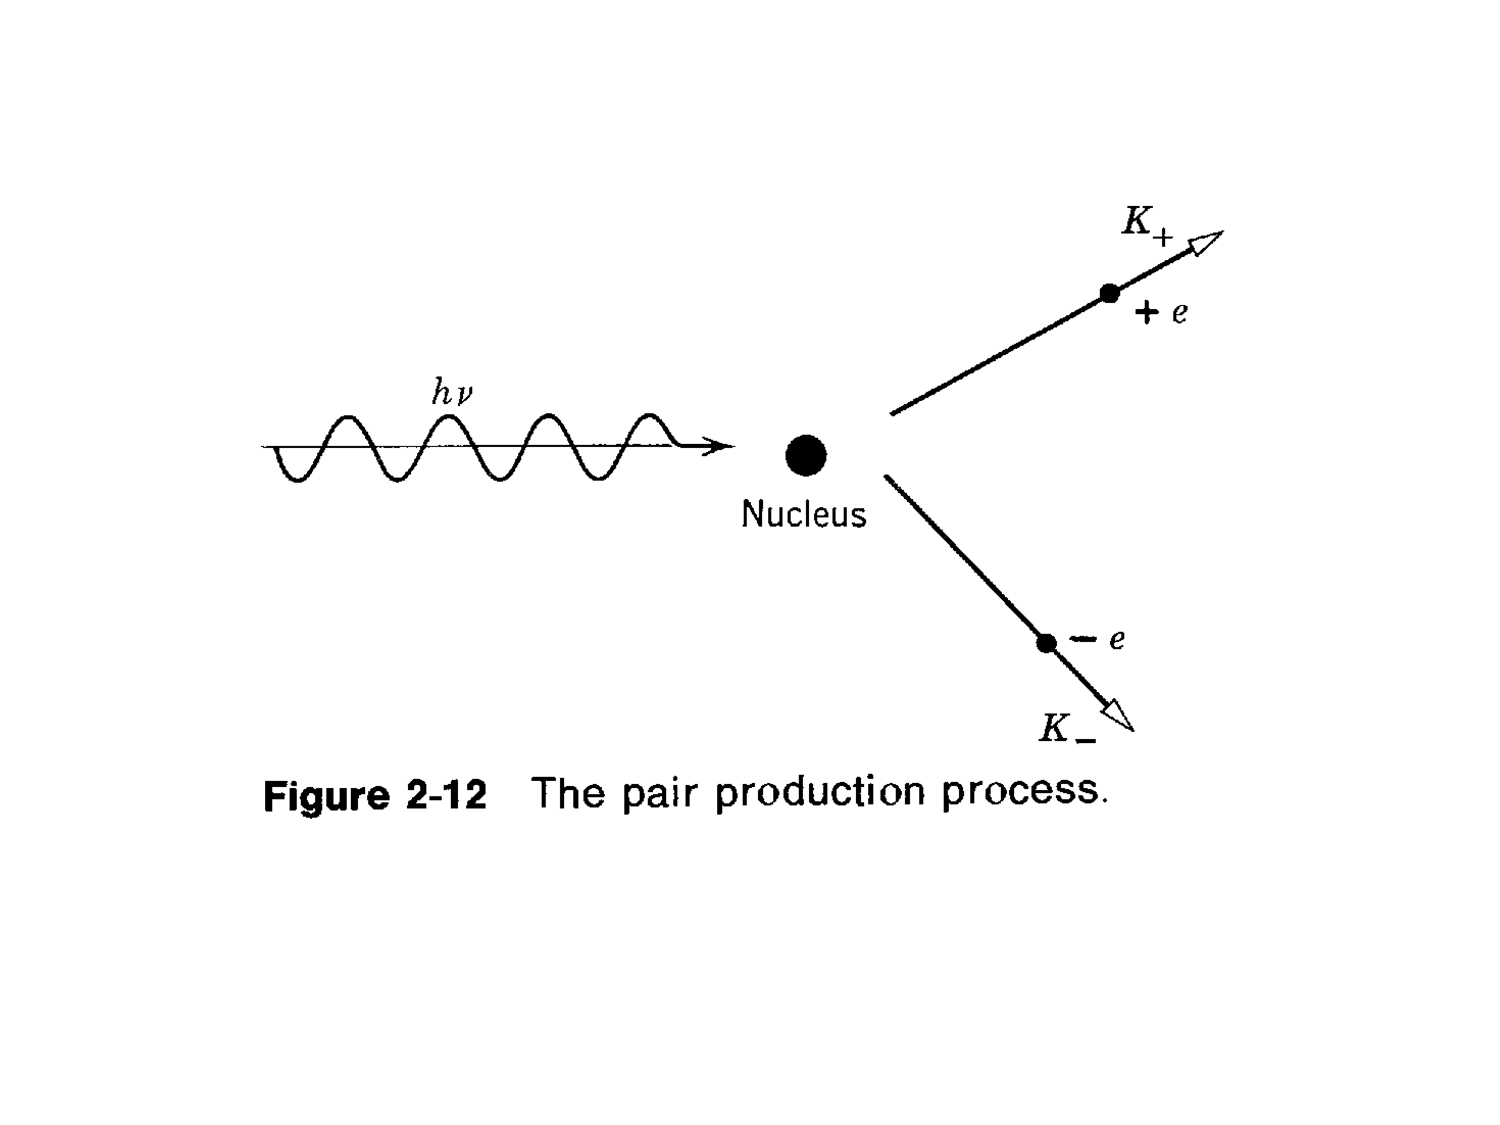
\includegraphics[scale=0.5]{/schema_pairproduction}
\caption{CAPTION}
\end{figure}

Eguagliando l'energia del fotone con la somma delle energie relativistiche delle due particelle si ottiene la cosiddetta \textit{energia di soglia}, ovvero l'energia minima del fotone per creare la coppia.

\begin{equation}
\begin{split}
& h\nu = E_- + E_+ = (m_0 c^2 + K_-) + (m_0 c^2 + K_+) = K_- + K_+ + 2m_0 c^2 \\
&\mbox{energia di soglia} \quad 2m_0c^2 = \SI{1.02}{MeV} \\
&\mbox{corrispondente a } \quad \lambda = \SI{0.012}{\AA} \quad \quad \mbox{da} \quad E = h\nu
\end{split}
\end{equation}
È un fenomeno che riguarda alte energie.

\subsection{Annichilazione di coppie}
Il fenomeno speculare al precedente si ha con l'annichilazione di coppie: in cui un elettrone ed un positrone inizialmente a riposo interagiscono formando radiazione elettromagnetica.

Considero il momento angolare di due fotoni:
\begin{equation}
\begin{split}
& 0 = \vec p_1 + \vec p_2 \quad \Rightarrow \quad \vec p_1 = - \vec p_2 \\
& p_1 = p_2 \\
& h \frac{ \nu_1}{c } = h \frac{ \nu_2}{c } \quad \Rightarrow \quad \nu_1 = \nu_2 = \nu
\end{split}
\end{equation}

I due fotoni hanno lo stesso momento e quindi gli si associa una stessa frequenza $\nu$.
Per la conservazione dell'energia:

\begin{equation}
m_0 c^2 + m_0 c^2 = h\nu + h\nu \quad \Rightarrow \quad 
h\nu = m_0 c^2 = \SI{0.511}{MeV} \quad \Rightarrow \quad
\lambda = \SI{0.024}{\AA}
\end{equation}

È un fenomeno che riguarda alte energie.






    %%
%% Author: dariochinelli
%% 2021-03-15
%%
\section{Cross section}

Quando una radiazione elettromagnetica (fotoni) interagiscono con la materia sono quattro i processi che consideriamo: \\
\textbf{Effetto fotoelettrico}: assorbimento totale del fotone \\
\textbf{Produzione di coppie}: assorbimento totale del fotone \\
\textbf{Scattering di Rayleigh}: diffusione del fotone in cui non perde energia \\
\textbf{Effetto Compton}: diffusione del fotone in cui perde energia \\

La cross section rappresenta la probabilità che questi effetti avvengono.
Per l'effetto fotoelettrico la cross section è:
\begin{equation}
\begin{split}
& \sigma_{PE} \quad \mbox{sezione d'urto fotoelettrica} \\
& N_{PE} = \sigma_{PE} I n
\end{split}
\end{equation}
Dove $I$ è il numero di fotoni del fascio incidente sulla lamina, $n$ è il numero di atomi per unità di area e quindi $N_{PE}$ definisce il numero di processi di assorbimento fotoelettrico.
Se la lamina la assumo molto sottile, posso assumere che gli atomi non si "schermino" tra loro.
La sezione d'urto mi esprime quanto efficacemente i fotoni vengono assorbiti dalla lamina.
$\sigma_{PE}$ deve quindi avere le dimensioni di un'area e possiamo dare un'interpretazione geometrica alla probabilità, dove considero un cerchio di area $\sigma_{PE}$ intorno al nucleo allora ho che ogni fotone che entra dentro questo cerchio interagirà con l'atomo.

\begin{figure}[h]
\centering
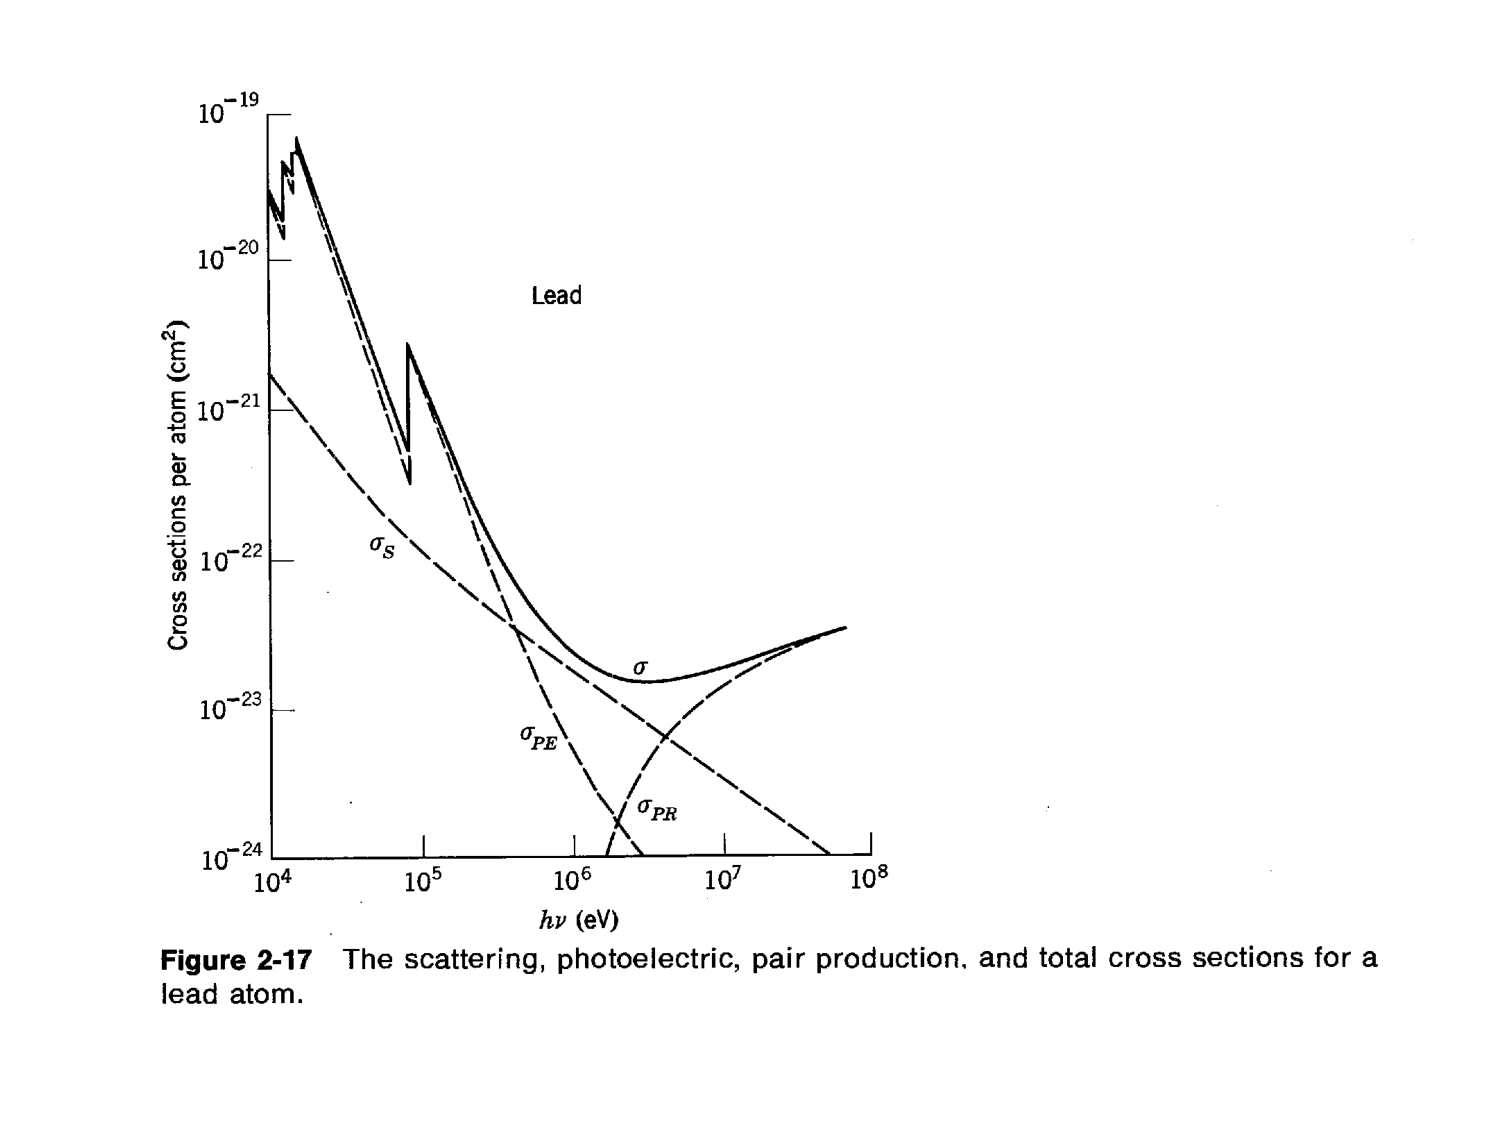
\includegraphics[scale=0.5]{/cross_section}
\caption{Cross section del Piombo (Lead). Si vede la cross section in funzione dell'energia del fotone. La linea continua rappresenta la cross section totale e linee tratteggiate sono le cross section riferite ai singoli processi. $\sigma_S$ rappresenta lo scattering e somma la diffusione alla Rayleigh e diffusione alla Compton. $\sigma_{PR}$ cross section produzione di coppie. $\sigma_{PE}$ effetto fotoelettrico.}
\end{figure}

Notare che i picchi nella curva di $\sigma_{PE}$ sono dovuti e corrispondono alle diverse energie di legame nell'atomo di piombo, quando l'energia del fotone diventa più piccola dell'energia di legame di un particolare tipo di elettroni non avviene più effetto fotoelettrico, si definiscono quindi delle \textit{soglie}.


    %%
%% Author: dariochinelli
%% 2021-04-05
%%


\section{Onde di Materia}
\subsection{Ipotesi di De Broglie}
Venne introdotto questo concetto nel 1924 nella tesi di dottorato di Louis De Broglie.
Le equazioni per la radiazione elettromagnetica di energia e quantità di moto sono rispettivamente
\begin{equation}
E = h\nu \quad \quad p = \frac{ h}{\lambda }
\end{equation}
dalla seconda si ricava la \textbf{lunghezza d'onda di De Broglie}
\begin{equation}
\lambda = \frac{ h}{p }
\end{equation}
che mette in relazione la natura ondulatoria della radiazione con la natura corpuscolare delle particelle.

\paragraph{Esempio}
Qual è la lunghezza d'onda di De Broglie di una palla di massa $ m =\SI{1}{kg}$ che si muove a una velocità $v = \SI{10}{m/s}$?
Soluzione:
\begin{equation}
\lambda = \frac{ h}{p } = \frac{ h}{m v } = \frac{ \SI{6.6e-34}{j.s}}{\SI{1}{kg} . \SI{10}{m/s} } = \SI{6.6e-35}{m} = \SI{6.6e-25}{\AA}
\end{equation}
Qual è la lunghezza d'onda di De Broglie di un elettrone avente energia cinetica \SI{100}{eV}?
\begin{equation}
\begin{split}
\lambda & = \frac{ h}{p } = \frac{ h}{\sqrt{2mK} } 
= \frac{\SI{6.6e-34}{j.s} }{\sqrt{ 2 \cdot \SI{9.1e-31}{kg} \cdot \SI{100}{eV} \cdot \SI{1.6e-19}{j / eV} } } \\
& = \frac{ \SI{6.6e-34}{j.s}}{\SI{5.4e-24}{kg.m/s} } = \SI{1.2e-10}{m} = \SI{1.2}{\AA}
\end{split}
\end{equation}

Da questi conti si vede quanto sia difficilmente osservabile la lunghezza d'onda di un oggetto macroscopico, che differisce da quella di un elettrone, come in esempio, di un fattore \SI{e-25}{}.
Dagli esperimenti di ottica si vede che la natura ondulatoria della luce si manifesta solo quando le grandezze in gioco sono confrontabili con la lunghezza d'onda della radiazione esaminata.
I cristalli, ad esempio, hanno una struttura la cui distanza inter-atomica è di una grandezza confrontabile con quella della lunghezza d'onda di un fascio di fotoni X, vedi legge di Bragg.
Una cosa analoga avviene con le onde di materia, potrò allora rivelare la natura ondulatoria di un elettrone solo se interagirà con qualcosa della dimensione dell'ordine dell'Amstrong, come visto sopra.
Non potrò vedere la natura ondulatoria della palla da $\SI{1}{kg}$ poiché non c'è niente in natura della dimensione di $\SI{e-25}{\AA}$ che possa far interferire questo oggetto.



\subsection{Esperimento di Davisson e Germer}
\paragraph{Apparato sperimentale} 
Facendo riferimento alla figura \ref{app_spe}: si ha un filamento di Tungsteno $(F)$ riscaldato che emette elettroni, i quali vengono accelerati, grazie ad una differenza di potenziale $(V)$, e fatti incidere su un bersaglio cristallino di Nichel $(C)$.
Ad un angolo $\theta$ viene posizionato un detector $(D)$, dove l'angolo può esser fatto variare per osservarne la diffusione.

\begin{figure}[h]
\centering
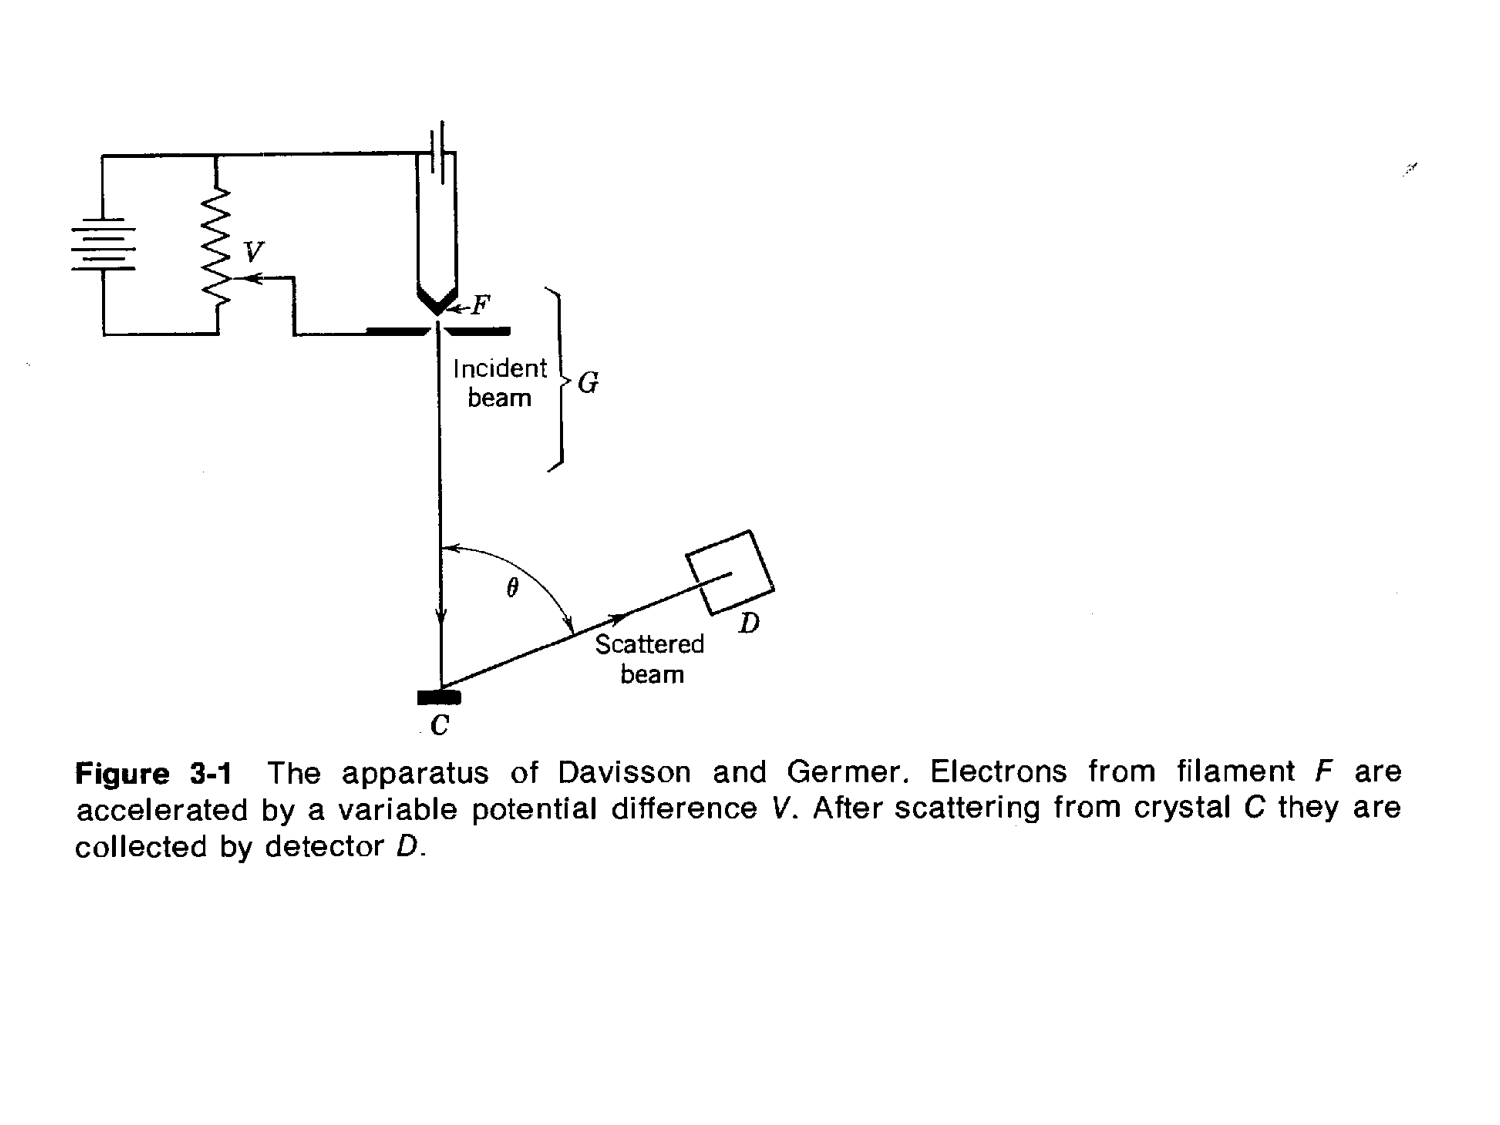
\includegraphics[scale=0.5]{/esp_devissongermer}
\caption{Schema della strumentazione utilizzata}
\label{app_spe}
\end{figure}
\begin{figure}[h]
\centering
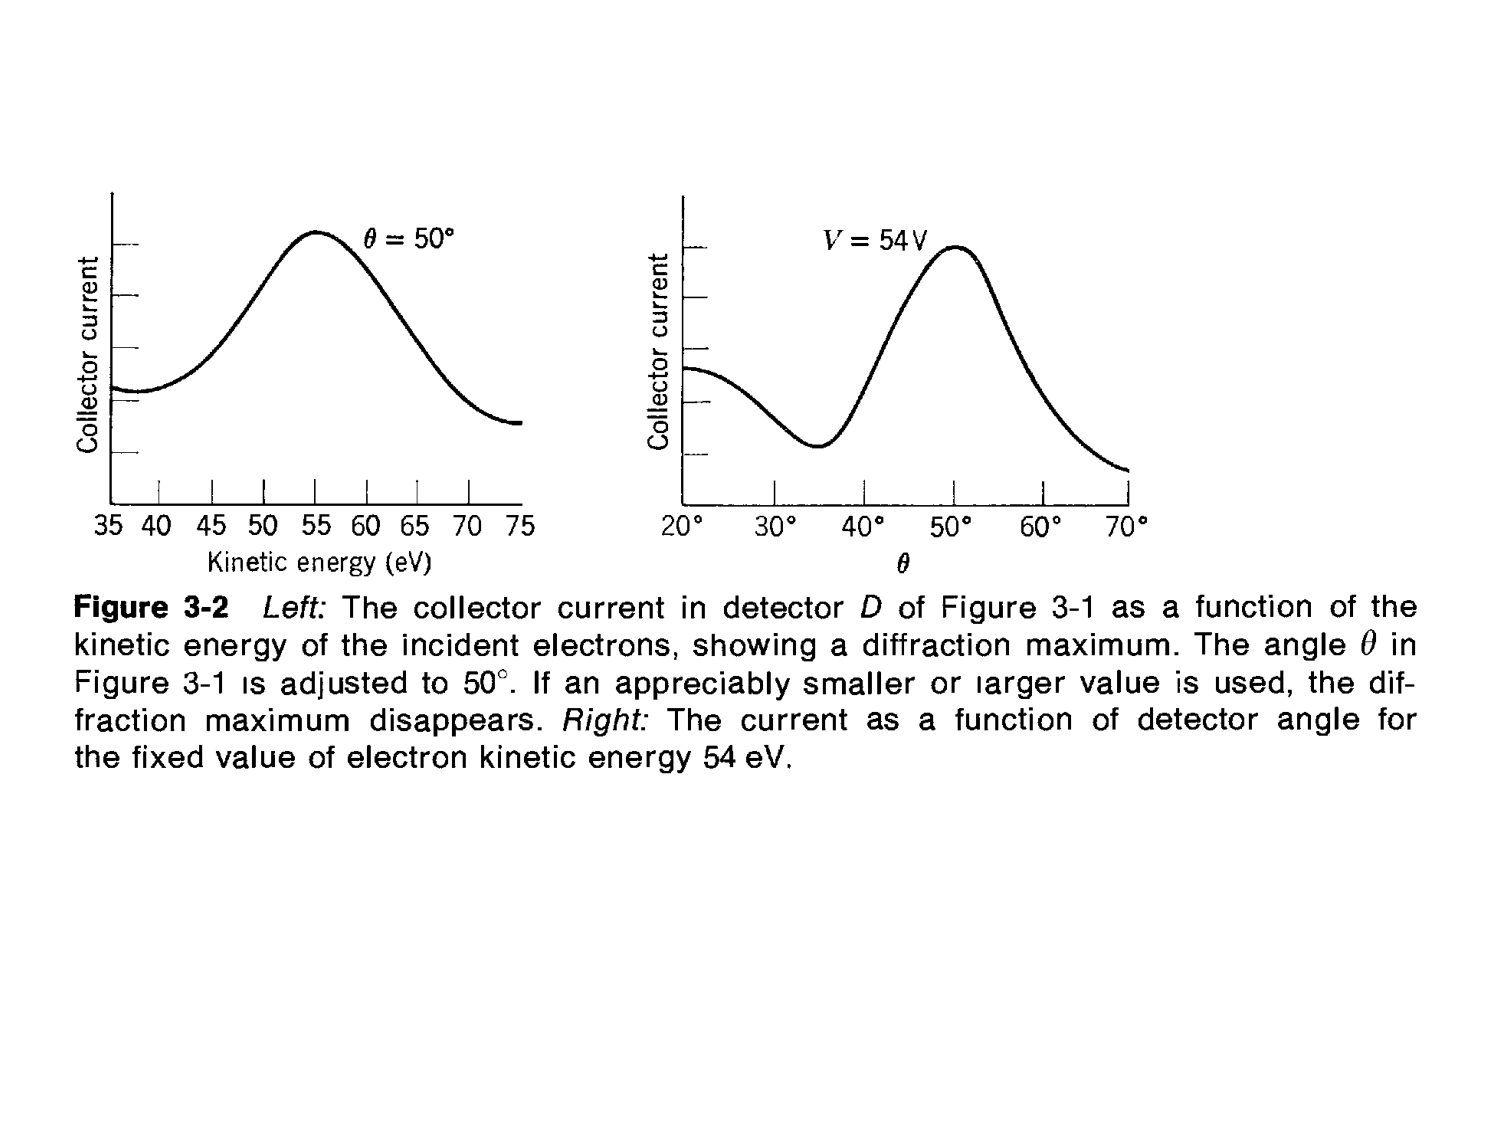
\includegraphics[scale=0.5]{/ris_esp_devissongermer}
\caption{Risultati sperimentali}
\label{res_spe}
\end{figure}

\paragraph{Risultati sperimentali}
Variando l'angolo di osservazione ed il potenziale applicato, quindi l'energia degli elettroni incidenti, osservarono gli andamenti evidenziati in figura \ref{res_spe} e notarono un picco nel segnale, quindi nell'intensità e quindi nel numero di elettroni diffusi per unità di tempo, in corrispondenza di un angolo $\theta = 50^{\circ}$.
Allo stesso modo fissando il potenziale a $V = \SI{54}{V}$ e facendo variare l'angolo, videro un picco in corrispondenza dell'angolo $\theta = 50^{\circ}$.
Con questa doppia misura i risultati si confermano reciprocamente.

\paragraph{Conclusioni}
Questo fenomeno non è spiegabile considerando l'elettrone come una particella.
Utilizzando una interpretazione ondulatoria del fascio di elettroni questo risultato lo si descrive come un fenomeno di interferenza:
i picchi risultano derivare dall'interferenza della particella-onda elettrone che attraversa la struttura cristallina.

Lo stesso fenomeno avviene anche utilizzando un fascio di elettroni molto debole, al punto da ipotizzare che solo un elettrone per volta attraversasse il cristallo, in modo quindi da escludere una interazione fra più elettroni e dimostrare che ogni singolo elettrone interferisce come onda.

Solo pochi anni prima era stata resa nota l'ipotesi di De Broglie, infatti Davisson e Germer individuarono questo fenomeno involontariamente, nemmeno ne erano al corrente.
Il loro scopo era far incidere gli elettroni sul campione di Nichel per acquisire informazioni sulla superficie di questo oggetto.
Fu Davisson che, dopo aver partecipato ad una conferenza sull'ipotesi di De Broglie, si accorse che c'era un collegamento tra il loro esperimento e tale ipotesi.

\paragraph{Teorie a confronto}
Considerando l'ipotesi di De Broglie, posso calcolare la lunghezza d'onda di De Broglie dell'elettrone nell'esperimento di Davisson e Germer
\begin{equation}
\lambda = \frac{ h}{p } = \frac{ h}{\sqrt{2mK} } 
= \frac{\SI{6.6e-34}{j.s} }{\sqrt{ 2 \cdot \SI{9.1e-31}{kg} \cdot \SI{54}{eV} \cdot \SI{1.6e-19}{j / eV} } } 
= \SI{1.67e-10}{m} = \SI{1.67}{\AA}
\end{equation}
Ed invece calcolando la lunghezza d'onda considerando la legge di Bragg trovo
\begin{equation}
\begin{split}
& 2 d \sin \varphi = n \lambda \\
& \lambda = 2 d \sin \varphi = 1.65 \AA
\end{split}
\end{equation}
trovo quindi un accordo molto buono tra le due teorie.





\subsection{Principio di complementarietà di Neils Bohr}
I modelli ondulatori e corpuscolari sono complementari: se una misura rivela il carattere ondulatorio allora nella stessa misura è impossibile determinarne il carattere corpuscolare, in un esperimento è quindi possibile osservare o la natura ondulatoria o la natura corpuscolare.

\paragraph{Ad esempio} nell'esperimento di Compton viene messa in evidenza la doppia natura, si utilizza uno stesso apparato ma è come se fossero due esperimenti in cascata in cui il primo, l'interazione della radiazione X con il target di carbonio, evidenzia la natura corpuscolare ed il secondo, in cui si osserva la diffrazione alla Bragg, quella ondulatoria.
Non c'è contraddizione con la complementarietà di Bohr perché non è un unico esperimento ma sono due esperimenti in cascata.


\paragraph{L'interpretazione probabilistica} è ciò che viene utilizzata per conciliare le due nature della radiazione e delle onde

\begin{equation}
\begin{split}
E & = A \sin \Bigl[ 2\pi \Bigl(  \frac{ x}{\lambda } - \nu t  \Bigr) \Bigr] \quad \mbox{Onda di radiazione} \\
\Psi & = A \sin \Bigl[ 2\pi \Bigl(  \frac{ x}{\lambda } - \nu t  \Bigr) \Bigr] \quad \mbox{Onda di materia}
\end{split}
\end{equation}

Il quadrato della funzione d'onda media descrive la \textbf{probabilità} di trovare una particella in un punto dello spazio in un certo momento.

Interpretazione nata dalla "Scuola di Copenhagen": quindi Heisenberg, Bohr, Born ...
si è imposta questo tipo di trattazione probabilistica, dopo varie discussioni e dibattiti.


 










    %%
%% Author: dariochinelli
%% 2020-09-29
%%


\section{Principio di indeterminazione di Heisemberg}
Il principio di Heisemberg è costituito da due parti: la prima parte riguarda la misura simultanea di momento e posizione di una particella mentre la seconda parte riguarda l'energia ed il tempo della misura.

Un esperimento non può determinare simultaneamente il valore esatto di una componente del momento $p_x$ e anche il valore esatto della posizione $x$, la precisione della misura è limitata dal processo stesso della misura, per cui
\begin{equation}
\begin{split}
& \Delta p_x \Delta x \ge \frac{ \hbar}{2 } \\
& \hbar = \frac{ h}{2\pi }
\end{split}
\end{equation}
È implicato il prodotto tra le incertezze per cui se l'incertezza sul momento è nulla, l'incertezza sulla posizione sarà infinita: $\Delta p_x = 0 \Rightarrow \Delta x = \infty$
Valgono le espressioni analoghe per le altre componenti
\begin{equation}
\Delta p_y \Delta y \ge \frac{ \hbar}{2 }
\quad\quad\quad\quad
\Delta p_z \Delta z \ge \frac{ \hbar}{2 }
\end{equation}
La seconda parte riguarda una relazione analoga tra l'energia ed il tempo richiesto per effettuare la misura:
\begin{equation}
\Delta E \Delta t \ge \frac{\hbar}{2}
\end{equation}
Il fatto che la costante di Planck sia tanto piccola non permette di vedere questi fenomeni nella vita ordinaria, quindi la fisica classica è ancora valida per descrivere oggetti macroscopici.


\paragraph{Esperimento concettuale di Bohr}
Cosa accade quando si desidera misurare con grandissima precisione la posizione di un elettrone?
Si può utilizzare un "microscopio" e illuminare l'elettrone con un fotone per poi vederlo mediante scattering Compton.
Osservare la particella non è un'azione priva di conseguenze poiché illuminandolo si produce un'interazione fotone-elettrone.
Tale perturbazione può essere ridotta al minimo, ma non eliminata, mandando un solo fotone per volta.
Si noti che anche in meccanica classica, l'osservatore disturba il moto del corpo in esame: se si studia il moto di un pianeta la massa dell'osservatore dà luogo ad un'interazione gravitazionale, ma data la piccolezza di questa massa rispetto al pianeta, tale interferenza è trascurabile.
In figura \ref{esp_bohr} è rappresentato l'esperimento mentale proposto da Bohr.

\paragraph{Momento angolare} Il momento angolare del fotone è dato dalla solita equazione
\begin{equation}
\begin{split}
p & = \frac{h}{\lambda} \\
p_x & = \frac{h}{\lambda} \sin\theta'
\end{split}
\end{equation}
e tale momento angolare potrà variare da $+p \sin \theta '$ a $-p \sin \theta '$, allora
\begin{equation}
\Delta p_x = 2p \sin \theta ' = 2(\frac{h }{\lambda }) \sin \theta '
\end{equation}
è l'incertezza sulla componente $x$ del momento angolare $p_x$ del fotone, che, per la conservazione del momento angolare, sarà uguale a quella dell'elettrone.

\paragraph{Posizione} Cosa si può dire sulla posizione $x$ dell'elettrone?
L'immagine di un microscopio è un reticolo di diffrazione, allora possiamo considerare l'ampiezza del massimo centrale di diffrazione come misura dell'incertezza della posizione del fotone, e anche questa misura è analoga per l'elettrone, si ottiene allora
\begin{equation}
\begin{split}
\Delta x = \frac{\lambda}{\sin \theta '}
\end{split}
\end{equation}

\begin{figure}[h]
\centering
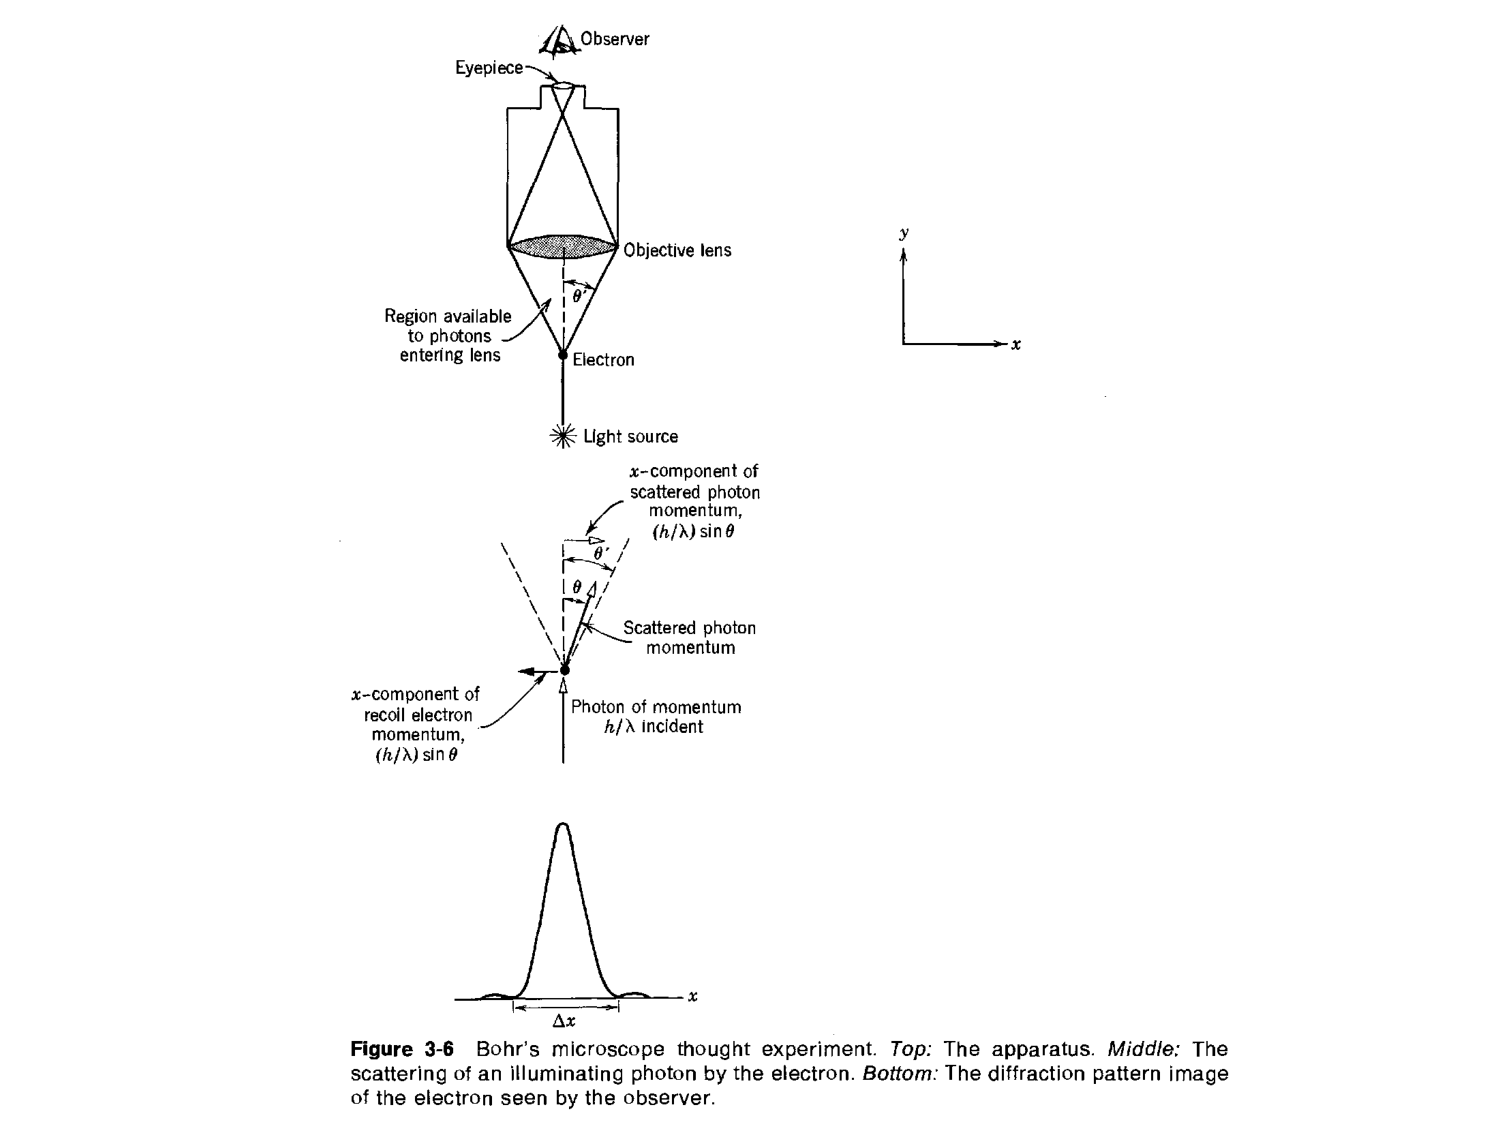
\includegraphics[scale=0.5]{/microsopio_bohr}
\caption{Schema dell'esperimento di Bohr}
\label{esp_bohr}
\end{figure}

\paragraph{Conclusione} Per ridurre l'incertezza sul momento dovrei aumentare la $\lambda$, viceversa per ridurre l'incertezza sulla posizione dovrei aumentare la $\lambda$, ovvero l'esatto contrario.
Facendo il prodotto tra le due incertezze trovo:
\begin{equation}
\Delta p_x \Delta x = (\frac{2h}{\lambda} \sin \theta ')(\frac{\lambda}{\sin \theta '}) = 2h > \frac{\hbar}{2}
\end{equation}
che non è propriamente il valore previsto dal Principio di Indeterminazione ma è comunque una costante.
Significa che far interferire un fotone con l'elettrone perturba la misura in un modo che non posso evitare, ovvero il \textit{principio di indeterminazione} riguarda strettamente l'incapacità di una misurazione infinitamente precisa.

Per quanto riguarda la seconda parte, scriviamo l'energia del fotone ed il tempo necessario per la misura
\begin{equation}
\begin{split}
E = \frac{ p_x^2}{2m }
& \quad\Rightarrow\quad  \Delta E = \Bigl(  \frac{ p_x}{m }  \Bigr) \Delta p_x = v_x \Delta p_x \\
x = v_x  t 
& \quad\Rightarrow\quad  \Delta t = \frac{ \Delta x}{v_x }
\end{split}
\end{equation}
dove $v_x$ è la velocità. 
In modo analogo all'equazione precedente, si trova
\begin{equation}
\Delta E \Delta t =  v_x \Delta p_x  \Delta x \frac{1}{v_x} = \Delta p_x \Delta x = 2h \ge \frac{ \hbar}{2 }
\end{equation}
quindi l'osservatore modifica in modo non trascurabile ed inevitabile la misura.

\paragraph{Esempio} La velocità di un proiettile di massa $m_p = \SI{0.05}{kg}$ e di un elettrone di massa $m_e = \SI{9.1e-31}{kg}$ sono uguali $v_x = \SI{300}{m/s}$, con un'incertezza di $10^{-4}$.
Con quale precisione posso localizzare la posizione di entrambi, se la posizione è misurata simultaneamente alla velocità?
Considero la direzione lungo l'asse $x$.

\underline{Per il proiettile:}
\begin{equation}
\begin{split}
& p = m v = \SI{5e-2}{kg} \cdot \SI{300}{m/s} = \SI{15}{kg.m/s} \\
& \Delta p = \SI{e-4}{} \cdot \SI{15}{kg.m/s} = \SI{1.5e-3}{kg.m/s} \\
& \Delta x = \frac{ h}{4\pi \Delta p } = \frac{ \SI{6.6e-34}{j.s}}{4\pi \cdot \SI{1.5e-3}{kg.m/s} } = \SI{3e-32}{m}
\end{split}
\end{equation}
che sono rispettivamente l'incertezza sulla quantità di moto e l'incertezza sulla posizione del proiettile, notiamo che l'incertezza rispetto alle dimensioni del proiettile ($\SI{e-2}{m}$) è pressoché trascurabile.

\underline{Per l'elettrone:}
\begin{equation}
\begin{split}
& p = m v = \SI{9.1e-31}{kg} \cdot \SI{300}{m/s} = \SI{2.7e-28}{kg.m/s} \\
& \Delta p = \SI{e-4}{} \cdot \SI{2.7e-28}{kg.m/s} = \SI{2.7e-32}{kg.m/s} \\
& \Delta x = \frac{ h}{4\pi \Delta p } = \frac{ \SI{6.6e-34}{j.s}}{4\pi \cdot \SI{2.7e-32}{kg.m/s} } = \SI{2e-3}{m} = \SI{0.2}{cm}
\end{split}
\end{equation}
che sono rispettivamente l'incertezza sulla quantità di moto e l'incertezza sulla posizione dell'elettrone, rispetto alle \textit{dimensioni} di un elettrone i 2 mm di incertezza rendono impossibile localizzarlo con precisione.

\paragraph{Derivazione del principio di indeterminazione}
Ricaviamo ora le relazioni del principio di indeterminazione combinando le equazioni di De Broglie e di Einstein, utilizzando le proprietà universali delle onde e le trasformate di Fourier, quindi
\begin{equation}
E = h \nu \quad\quad\quad p = \frac{ h}{\lambda }
\label{dualita_oc}
\end{equation}
Per ottenere una funzione d'onda che sia diversa da zero solo dove è localizzata la particella devo considerare un gruppo di onde e non una sola onda monocromatica.
Ad esempio un gruppo di due onde è così costruito
\begin{equation}
\begin{split}
& \Psi(x,t) = \Psi_1(x,t) + \Psi_2(x,t) \\
& \Psi_1(x,t) = \sin \Bigl[  2\pi (kx -\nu t)  \Bigr] \\
& \Psi_1(x,t) = \sin \Bigl[  2\pi ((k + dk) x - (\nu +d\nu) t)  \Bigr]
\end{split}
\label{eq_onde_gen}
\end{equation}
Per localizzare maggiormente lo spazio in cui trovare la particella $\Delta x$devo aumentare il range di $\Delta k$.
\begin{figure}[h]
\centering
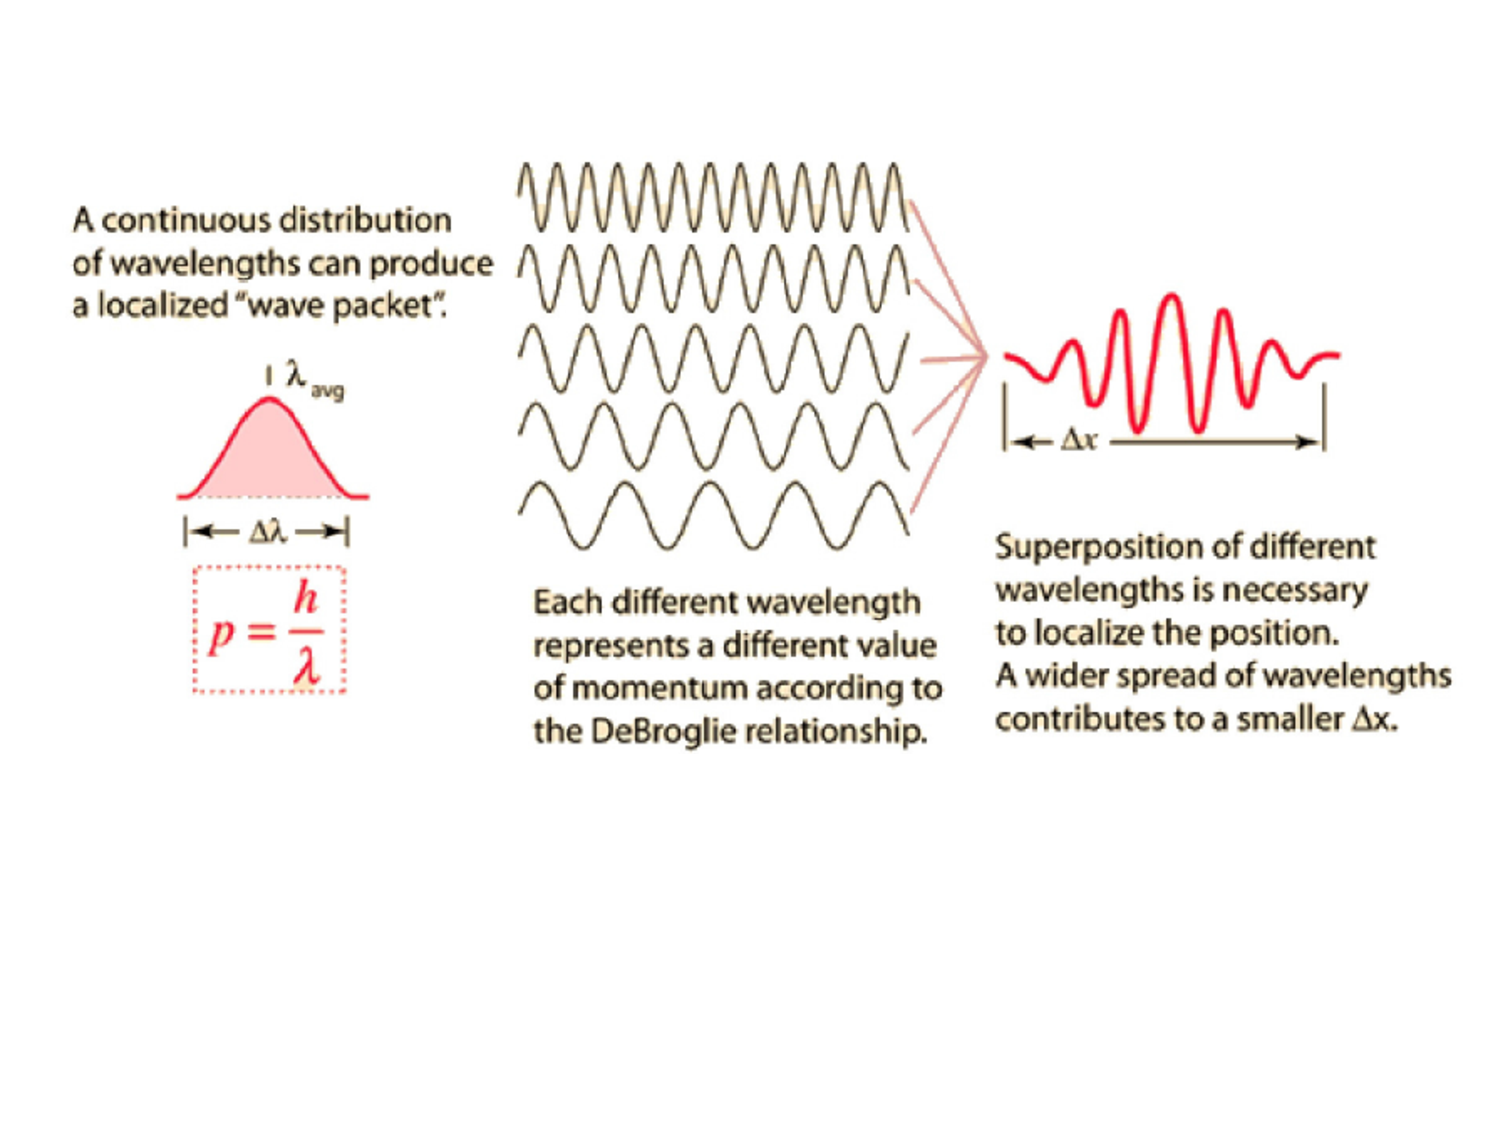
\includegraphics[scale=0.5]{/wave_packet}
\caption{Come produrre un'onda localizzata}
\end{figure}

\paragraph{Analisi di Fourier} 
queste sono le relazioni universali per tutte le onde
\begin{equation}
\begin{split}
& \Delta x \Delta k \ge \frac{ 1}{4\pi } \\
& \Delta t \Delta \nu \ge \frac{ 1}{4\pi }
\end{split}
\label{eq_univ}
\end{equation}
Partendo dalle equazioni \ref{eq_univ} universali delle onde, dalle proprietà delle onde e dalle espressioni \ref{dualita_oc} troviamo il risultato cercato
\begin{equation}
\begin{split}
& \Delta x \Delta k = \Delta x \Delta \frac{1}{\lambda} = \Delta x \Delta \frac{p}{h}  \ge \frac{1}{4\pi} 
\quad\Rightarrow\quad \Delta x \Delta p \ge \frac{\hbar}{2} \\
& \Delta t \Delta \nu = \Delta t \Delta \frac{E}{h} \ge \frac{1}{4\pi} 
\quad\Rightarrow\quad  \Delta t \Delta E \ge \frac{\hbar}{2}
\end{split}
\end{equation}
Ottenendo quindi le relazioni del principio di indeterminazione:
\begin{equation}
\Delta p \Delta x \ge \frac{\hbar}{2} 
\quad\quad\quad\quad
\Delta E \Delta t \ge \frac{\hbar}{2}
\end{equation}

\paragraph{Velocità di gruppo delle onde}
Le equazioni \ref{eq_univ} derivano dallo studio della velocità di gruppo delle onde.
La velocità di propagazione di un'onda è $W=\lambda \nu$ per De Broglie è $$W = \lambda \nu = \frac{h}{p} \frac{E}{h} = \frac{E}{p}$$
Assumendo che la particella si muova a velocità non relativistiche $v$ in una regione definita, si ottiene che:
\begin{equation}
W = \frac{E}{p} = \frac{1}{2} \frac{m v^2}{m v} = \frac{v}{2}
\end{equation}
tuttavia questo risultato non è buono poiché sembra affermare che le onde di materia non siano capaci di "tenere il passo" rispetto alla particella...
Si immagini che la particella si muova libera lungo l'asse x, e si associ a tale moto un'onda di materia. Al tempo $t=0$ si registra la sua ampiezza.
Si associa quindi una funzione $\Psi (x,t)$.
Consideriamo ora la velocità di gruppo di tali onde, data dalla $g=\frac{d \nu}{d k}$ con $k= \lambda^{-1}$ e si consideri quindi la generica onda.
Si può trattare un gruppo di onde come una semplice somma di più onde, come in equazione \ref{eq_onde_gen}, da cui si ottiene 
\begin{equation}
\Psi (x, t) = 2 \cos [ 2 \pi ( \frac{dk}{2} x - \frac{d\nu}{2} t ) ] \sin [ 2\pi ( \frac{2k + dk}{2} x - \frac{2\nu + d\nu}{2} t ) ]  
\end{equation}
e se considero $ d\nu \ll 2\nu $ e $ dk \ll 2k $
\begin{equation}
 \Psi (x, t) = 2 \cos [ 2 \pi ( \frac{dk}{2} x - \frac{d\nu}{2} t ) ] \sin [ 2 \pi ( k x - \nu t )] 
\end{equation}
Dunque due onde con una lieve differenza di frequenza e di lunghezza d'onda interferiscono e producono una successione di gruppi che si muovono lungo l'asse $x$.
La velocità $W$ delle onde individuali può essere valutata considerando il secondo fattore di $\Psi (x, t)$, e la velocità $g$ di gruppo può essere trovata dal primo fattore.
Ciò non cambia considerando più di due onde.
$$ g = \frac{d\nu}{2}\frac{2}{dk} = \frac{d\nu}{dk} $$
\begin{equation}
\begin{split}
& \nu= \frac{E}{h} \rightarrow d\nu = \frac{d E}{h} \\
& k = \frac{1}{\lambda} = \frac{p}{h} \rightarrow dk=\frac{d p}{h}
\end{split}
\end{equation}
si ottiene così la velocità di gruppo: 
\begin{equation}
g = \frac{d E}{d p} = \frac{m v dv}{m dv} = v 
\quad\Rightarrow\quad  g = v
\end{equation}







    %%
%% Author: dariochinelli
%% 2021-04-07
%%


\section{Modelli atomici}
Analizziamo di seguito i modelli atomici dalla fisica classica fino alla \textit{"old quantum theory"}.


\subsection{Modello di Thomson}
Nel 1904 Thomson propose il modello atomico detto a \textit{panettone}, per il quale l'atomo è costituito da una distribuzione di carica positiva diffusa dove all'interno si trovano inserite le cariche negative.
Tale atomo, complessivamente neutro, risulterebbe sostanzialmente pieno e gli elettroni sarebbero fissi nelle posizioni di equilibrio. 
Nello stato di più bassa energia gli elettroni sono fissi in posizioni di equilibrio, mentre per atomi eccitati (a cui viene fornita energia ad esempio riscaldando il materiale) si ha una vibrazione intorno alla posizione di equilibrio emettendo onde elettromagnetiche.
All'epoca si considerava che il \textbf{raggio atomico} fosse dell'ordine di $\SI{1}{\AA}$, stimato considerando la densità, il peso atomico ed il numero di Avogadro. \\
Questo modello ha molti problemi, tra cui non riuscire a spiegare completamente gli spettri atomici e l'esperimento di scattering delle particelle alfa.
Fu Rutherford a smentire il modello a \textit{panettone}.

\paragraph{Esperimento di Rutherford (1911): scattering di particelle $\alpha$}
Venne fatto incidere un fascio di particelle $\alpha$, atomo di Elio doppiamente ionizzato di carica positiva, emesso da una sorgente radioattiva, contro una sottile lamina d'oro, il cui spessore era di poche migliaia di atomi.
\begin{figure}[h]
\centering
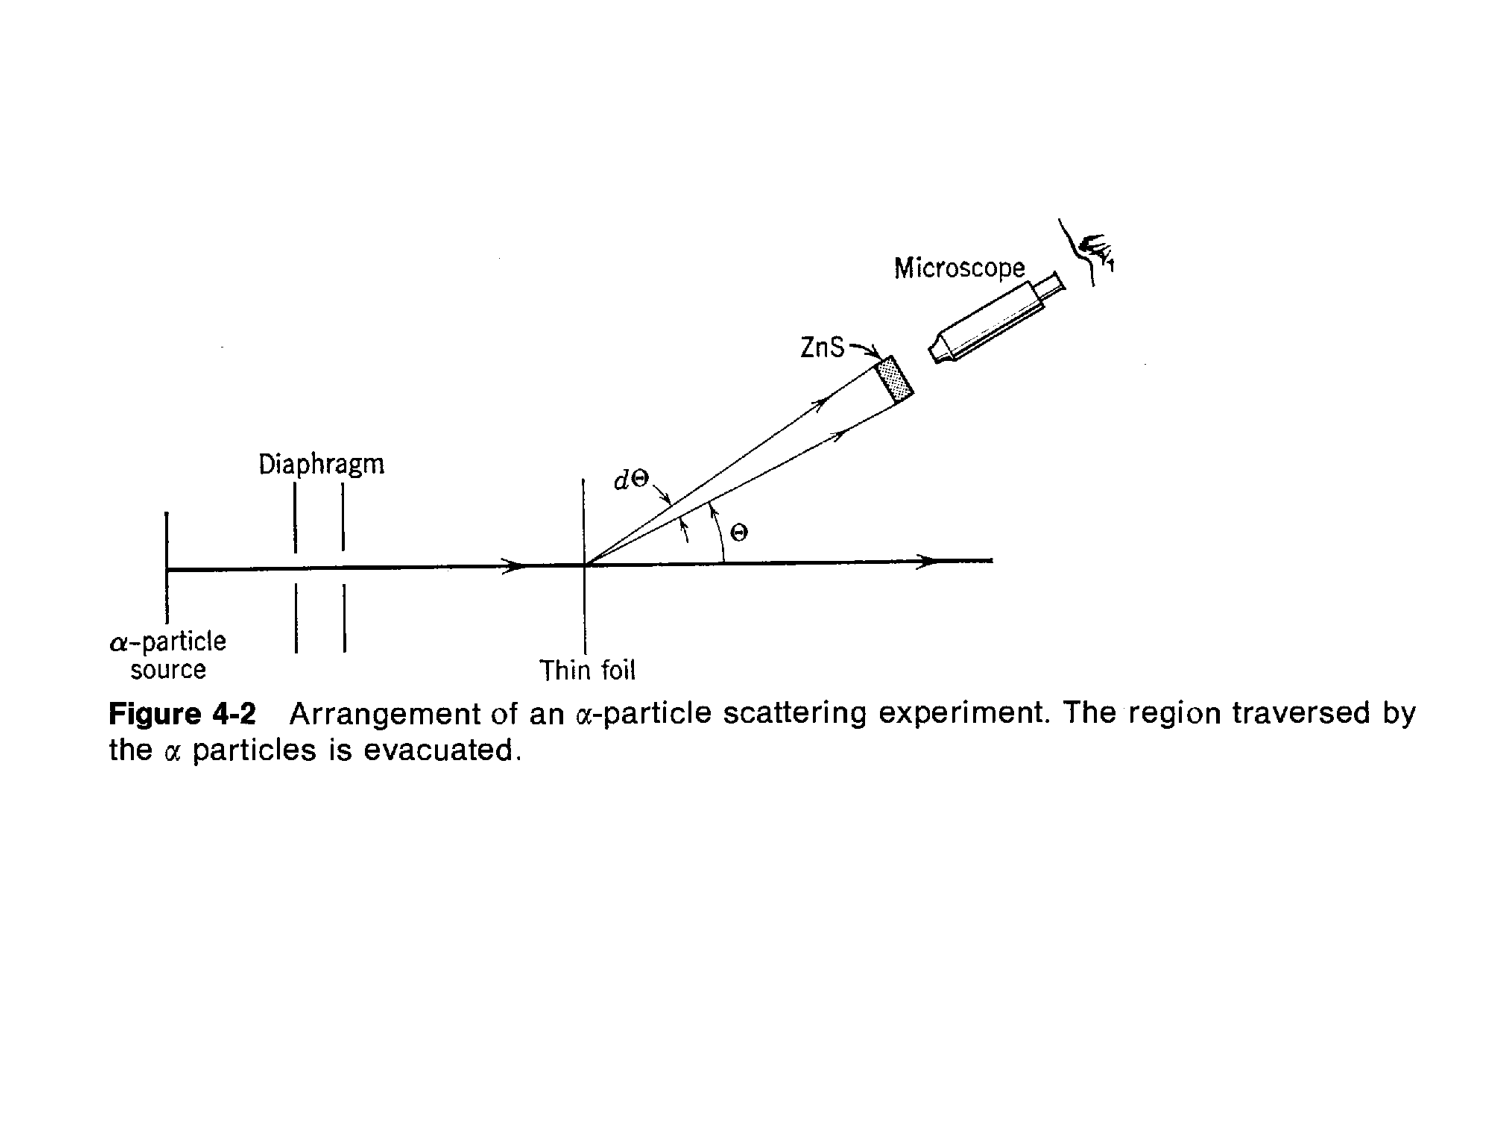
\includegraphics[scale=0.55]{/ruth_alpha}
\caption{Schema esperimento di Rutherford}
\end{figure}
Venne posizionato uno schermo fluorescente (ZnS) tutto intorno alla lamina d'oro, in modo da evidenziare il passaggio di ogni particella alfa.
In questo modo fu possibile ricostruire la traiettoria percorsa dalle particelle dopo la diffusione con la lamina.
Secondo il modello di Thomson le particelle avrebbero dovuto attraversare il foglio d'oro ed uscire con una traiettoria variata al più di pochi gradi, quindi poco diffuse.

\begin{figure}[h]
\centering
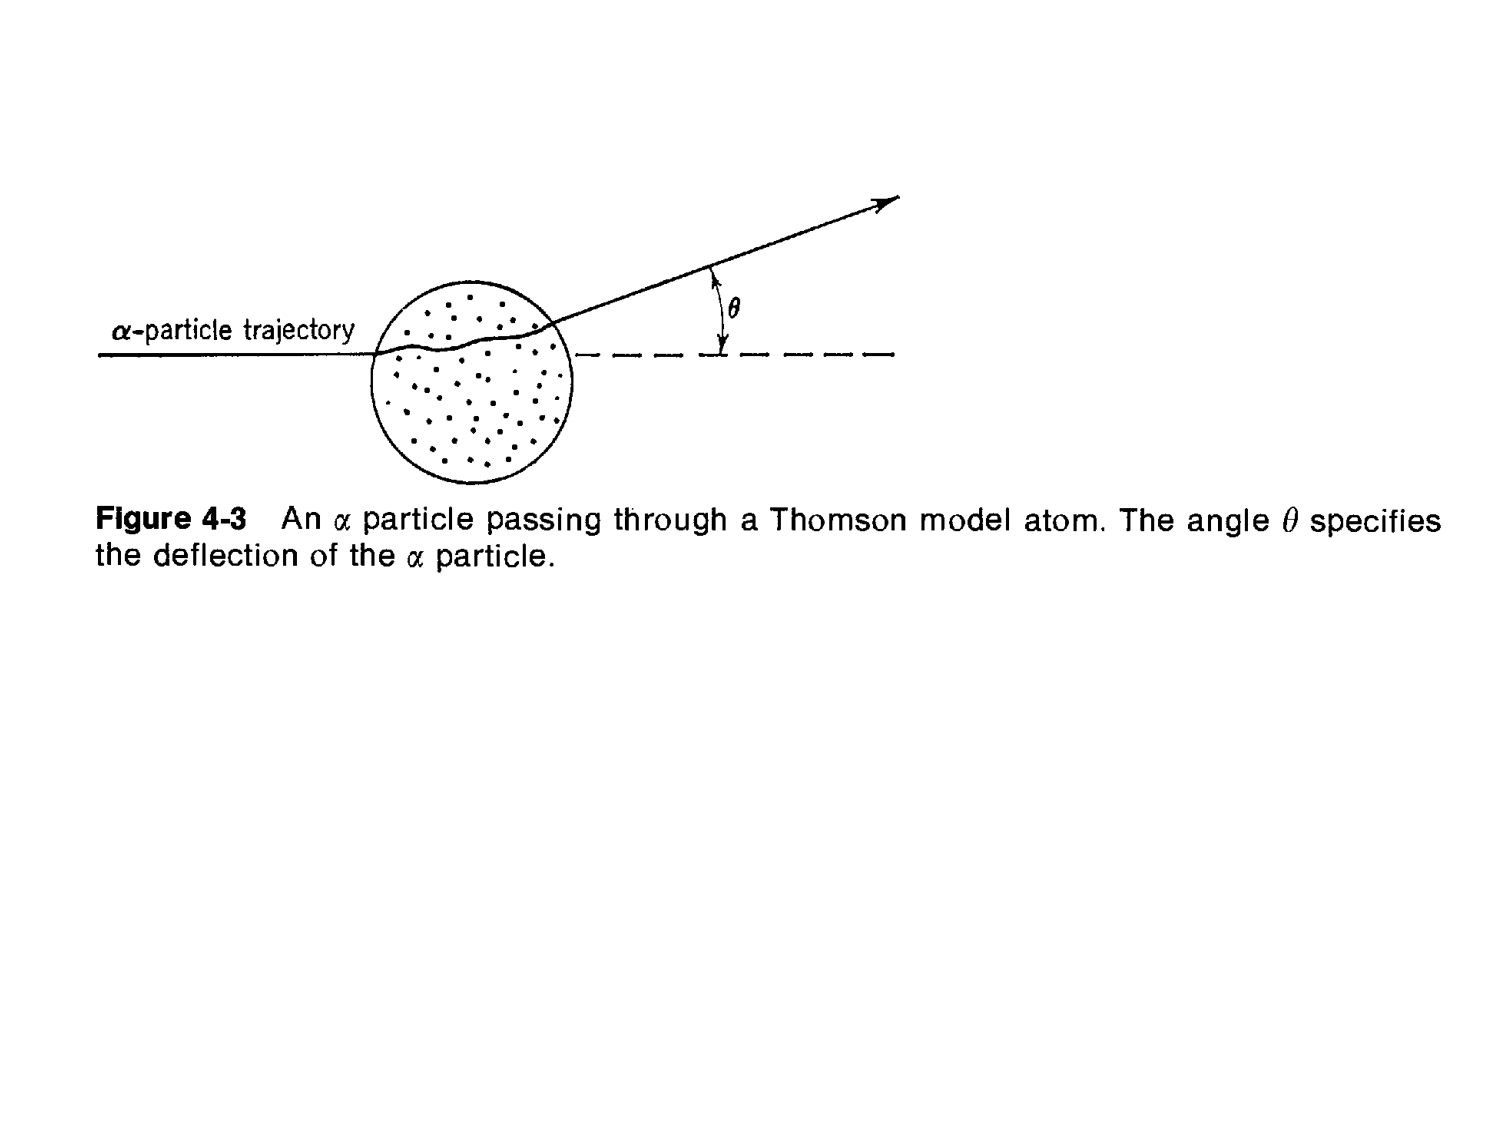
\includegraphics[scale=0.55]{/thomson_alpha}
\caption{Interazione della particella alfa con il nucleo nel modello di Thomson}
\end{figure}
Misurando la diffusione delle particelle si poterono ricavare informazioni sulla distribuzione della carica elettrica all'interno dell'atomo.
La formula seguente unisce l'angolo di scattering $\Theta$, ovvero l'angolo di deflessione totale della particella nel passaggio dell'intera lamina e l'angolo della deflessione $\theta$ causata da un atomo solo.
Sia $N$ il numero di atomi che deflettono una particella alfa nel suo passaggio attraverso la lamina.
\begin{equation}
\Bigl(  \overline{ \Theta^2 }  \Bigr)^{ \frac{ 1}{2 } } = \sqrt{N} \Bigl(  \overline{ \theta^2 }  \Bigr)^{ \frac{ 1}{2 } }
\end{equation}
$N(\Theta)d\Theta$ esprime il numero di particelle diffuse in un angolo $d\Theta$
\begin{equation}
N(\Theta)d\Theta = \frac{2 I \Theta}{\overline{\Theta^2}} e^{-{\Theta^2}/{\overline{\Theta^2}}} d\Theta
\end{equation}
In cui $I$ rappresenta il numero di particelle $\alpha$ che attraversano la lamina.
L'esponenziale descrive come il numero di particelle diffuse diminuisca drasticamente all'aumentare dell'angolo di scattering.
\begin{figure}[h]
\centering
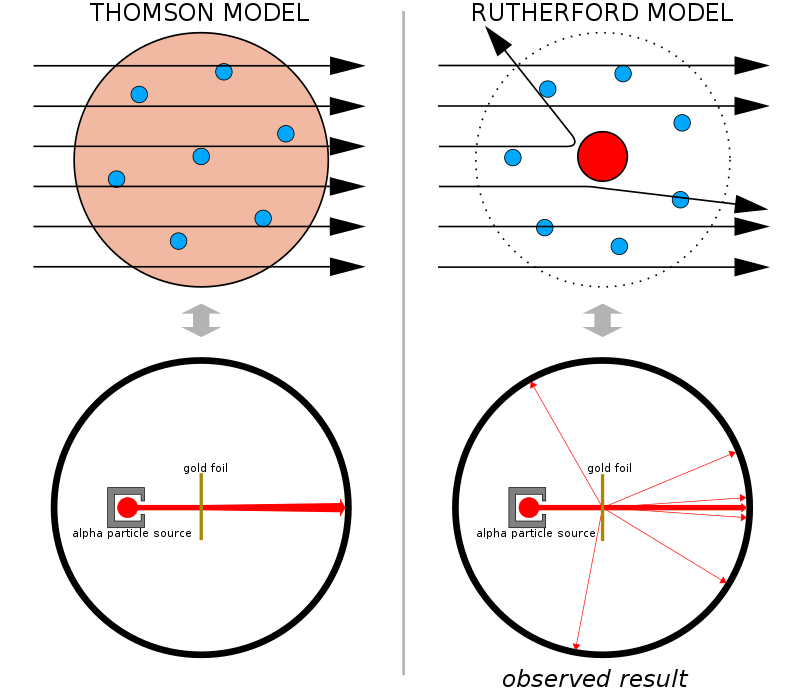
\includegraphics[scale=0.4]{/Geiger_Marsden_experiment_expectation_and_result}
\caption{Confronto dei risultati previsti dai due modelli}
\end{figure}
Questa formula si ottiene trascurando le interazioni coulombiane tra le particelle $\alpha$ e gli elettroni (la cui massa è assai piccola) e si conta solo la deflessione dovuta alla parte positiva dell'atomo. \\
Secondo Thomson, se la carica positiva fosse stata distribuita in modo continuo, non sarebbe possibile avere $\theta$ grandi poiché deve essere $\theta \le \SI{e-4}{rad}$.

A questo proposito si consideri l'\textbf{esperimento di Geiger e Marsden (1909)}.
Sperimentalmente venne accertato che alcune particelle, 1 su 8000, venivano diffuse ad angoli maggiori di $\frac{ \pi}{2 }$, evento completamente imprevisto da Thomson, ma in accordo con Rutherford.

\paragraph{Esempio} 
dato lo spessore della lamina d'oro pari a \SI{e-6}{m} e sia l'angolo medio di scattering pari a $(\overline{\Theta^2})^{1/2} = 2\cdot 10^{-2} RAD$ , si calcoli $(\overline{\theta^2})^{1/2}$
\begin{equation}
\begin{split}
N = \frac{\SI{e-6}{m}}{\SI{e-10}{m}} = \SI{e-4}{} 
\quad\Rightarrow\quad 
(\overline{\theta^2})^{1/2} = \frac{(\overline{\Theta^2})^{1/2}}{\sqrt{N}} = \frac{2\cdot 10^{-2}}{10^{2}} = \SI{2e-4}{rad}
\end{split}
\end{equation}


\subsection{Modello di Rutherford}
Tutta la carica positiva è concentrata nel \textit{nucleo} di raggio $r = \SI{e-14}{m}$.
In questo modello una particella alfa che passi molto vicino ad esso può essere scatterata da una forza repulsiva ed essere deviata di angoli molto ampi.
Rutherford calcolò la distribuzione angolare assumendo che lo scattering fosse solo tra la particella $\alpha$ ed il nucleo, ignorando l'interazione coulombiana con gli elettroni: gli elettroni avendo massa molto più piccola producono deflessioni a piccoli angoli.
Considera quindi solo la forza coulombiana tra la particella $\alpha$ e il nucleo, considerandolo fisso nello spazio durante l'urto ed imponendo che la particella non possa entrare nel nucleo: equivale a considerare i due oggetti come puntiformi.
\begin{figure}[h]
\centering
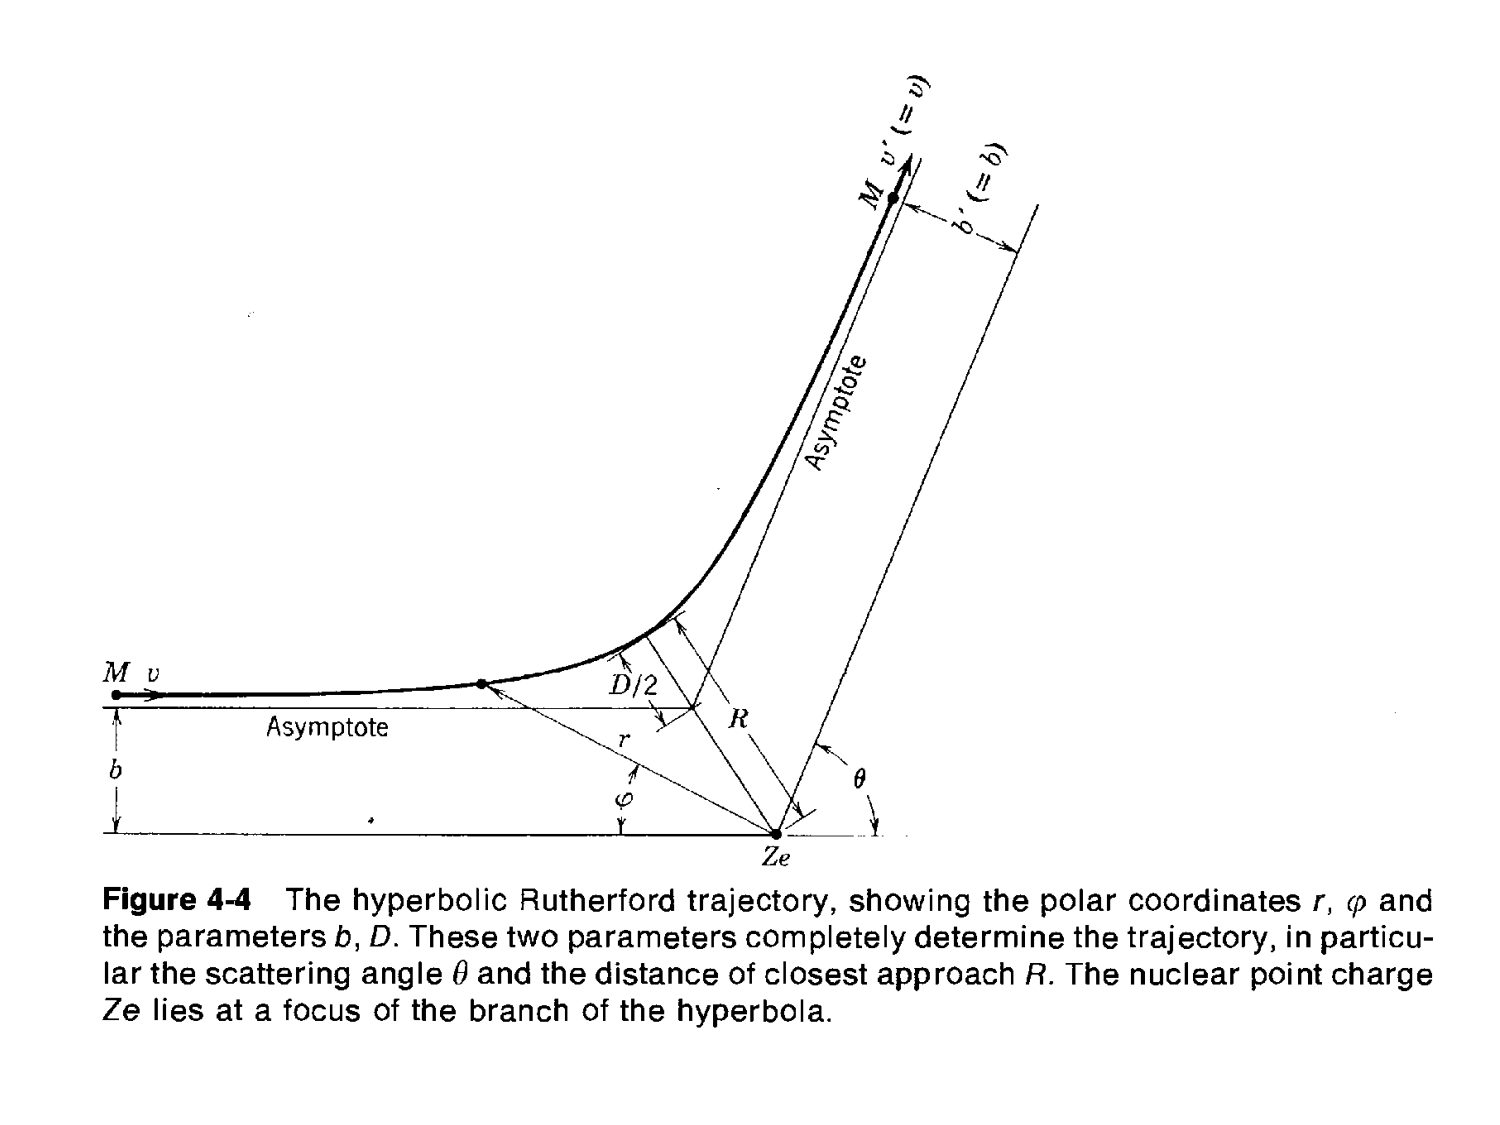
\includegraphics[scale=0.5]{/iperbole}
\caption{Iperbole di deflessione della particella da parte del nucleo}
\end{figure}
In cui notiamo che i moduli delle velocità iniziale e finale della particella $\alpha$ siano uguali.
L'angolo $\varphi$ descrive la posizione in coordinate polari.
L'angolo $\theta$ è l'angolo di deflessione.
$D$ è una costante che corrisponde alla distanza di avvicinamento minima in una collisione frontale, ovvero dove l'energia potenziale coulombiana è uguale all'energia cinetica della particella (vedi eq \ref{v_k}).
\begin{equation}
F = \frac{z Z e^2}{4\pi \varepsilon_0 r^2}
\end{equation}
da cui si ottiene
\begin{equation}
\frac{1}{r} = \frac{\sin \phi}{b} + \frac{D}{2 b^2} ( \cos \phi - 1 )
\end{equation}
dove $b$ è il parametro di impatto
\begin{equation}
\begin{split}
& D = \frac{1}{4\pi \varepsilon_0} \frac{z Z e^2}{M r^2/2} \\
& \frac{1}{4\pi \varepsilon_0} \frac{z Z e^2}{D} = \frac{ 1}{2 } M v^2
\end{split}
\label{v_k}
\end{equation}

L'angolo $\theta$ di scattering segue il valore di $\varphi$ quando $r \rightarrow \infty $ e ponendo $\theta = r - \varphi $, da cui:
\begin{equation}
\begin{split}
& \lim_{x\to\infty} \bigg\{  \frac{1}{r} = \frac{\sin(r - \theta)}{b} + \frac{D}{2 b^2} [ \cos (r - \theta) - 1 ] \bigg\} = 0 \\
& \sin \theta = \frac{D}{2 b} (\cos \theta + 1) \\
& \frac{2 b }{D} = \frac{\cos \theta + 1}{\sin \theta} = \frac{ [\cos^2 (\theta /2) - \sin^2 (\theta /2) ] + [ \sin^2(\theta /2) + \cos^2(\theta /2) ] }{  2 \sin(\theta /2) \cos(\theta /2)  }
\end{split}
\end{equation}

\begin{equation}
\cot(\theta /2) = \frac{2 b}{D}
\label{angolo_di_scattering}
\end{equation}
Da cui si deduce che se nello scattering di una particella alfa con un singolo nucleo è nel range da $b$ a $b + db$ allora l'angolo di scattering sarà nel range $[\theta, \theta + d\theta]$.
Un'altra formula importante è quella della distanza di avvicinamento minima è data da
\begin{equation}
\begin{split}
& R = \frac{ D}{2 } \Bigl[ 1 + \frac{ 1}{\sin\Bigl(  \frac{\theta}{2 }  \Bigr) } \Bigr] \\
& \mbox{t.c. se} \quad \theta \to \pi \quad (b=0) \quad \Rightarrow \quad R \to D \\
& \mbox{t.c. se} \quad \theta \to 0 \quad (b=\infty) \quad \Rightarrow \quad R \to \infty
\end{split}
\end{equation}

Ebbene il problema di calcolare il numero $ N(\Theta) d\Theta$ delle particelle alfa scatterate nel range angolare $[\Theta, \Theta +d\Theta]$ nell'attraversare la lamina è equivalente al problema di calcolare il numero di quelle incidenti, con un parametro d'impatto nel range $[b, b +db]$.
Da cui si ottiene la formula di Rutherford:
\begin{equation}
N(\Theta)d\Theta = \biggl( \frac{1}{4\pi \varepsilon_0} \biggr) ^2  \biggl( \frac{z Z e^2}{2 M v^2} \biggr)^2  \frac{ 2 \pi I \rho t  \sin\Theta d\Theta }{ \sin^4(\Theta/2) }
\label{scattering_rutherford}
\end{equation}
Dove $I$ è il numero di particelle alfa che incidono sulla lamina di spessore $t$.
Anche questa formula prevede una decrescita del numero di particelle all'aumentare dell'angolo, ma in modo più lieve rispetto al modello precedente di Thomson.
Da questo modello si vede che è possibile un \textit{back scattering} anche nell'interazione con un solo nucleo.

Si vede che, se comparato al modello di Thomson, sebbene in entrambi i casi il fattore angolare decresce rapidamente all'aumentare di $\Theta$, tale decrescenza è decisamente più precisa per le predizioni di Rutherford.
La formula di scattering di quest'ultimo è tale che il numero di $dN$ di particelle $\alpha$ scatterate in un angolo solido $d \Omega$ ad un angolo di scattering sia:
\begin{equation}
dN =  \frac{ d\sigma }{d\Omega} I n d\Omega
\end{equation}
Dove $I$ è il numero di particelle alfa incidenti sulla lamina sottile contenente $n$ nuclei per centimetro quadrato.
La definizione è analoga alla definizione di \textit{cross section}
\begin{equation}
N = \sigma I n
\end{equation}
e considerando che $d\Omega = 2\pi\sin\Theta d\Theta$, si riscrive la formula di scattering come differenziale
\begin{equation}
\begin{split}
& dN =  \biggl( \frac{1}{4\pi \varepsilon_0} \biggr) ^2  \biggl( \frac{z Z e^2}{2 M v^2} \biggr)^2  \frac{ I e t 2 \pi \sin\Theta d\Theta }{ \sin^4(\Theta/2) } \\
& \frac{ds}{d\Omega} = \biggl( \frac{1}{4 \pi \varepsilon_0} \biggr)^2  \biggl( \frac{z Z e^2}{2 M v^2} \biggr)^2  \frac{ 1 }{ \sin^4(\Theta/2) }
\end{split}
\end{equation}

\paragraph{Problemi nel modello di Rutherford}
Il modello di Rutherford non era però in grado di spiegare alcuni fenomeni.
\begin{enumerate}
\item Alte energie di impatto \\
Degli esperimenti in cui si fa variare l'energia delle particelle incidenti evidenziarono che oltre un certo valore di energia pari a $\SI{27.5}{MeV}$ il modello di Rutherford è completamente in disaccordo con i dati sperimentali.
\begin{figure}[h]
\centering
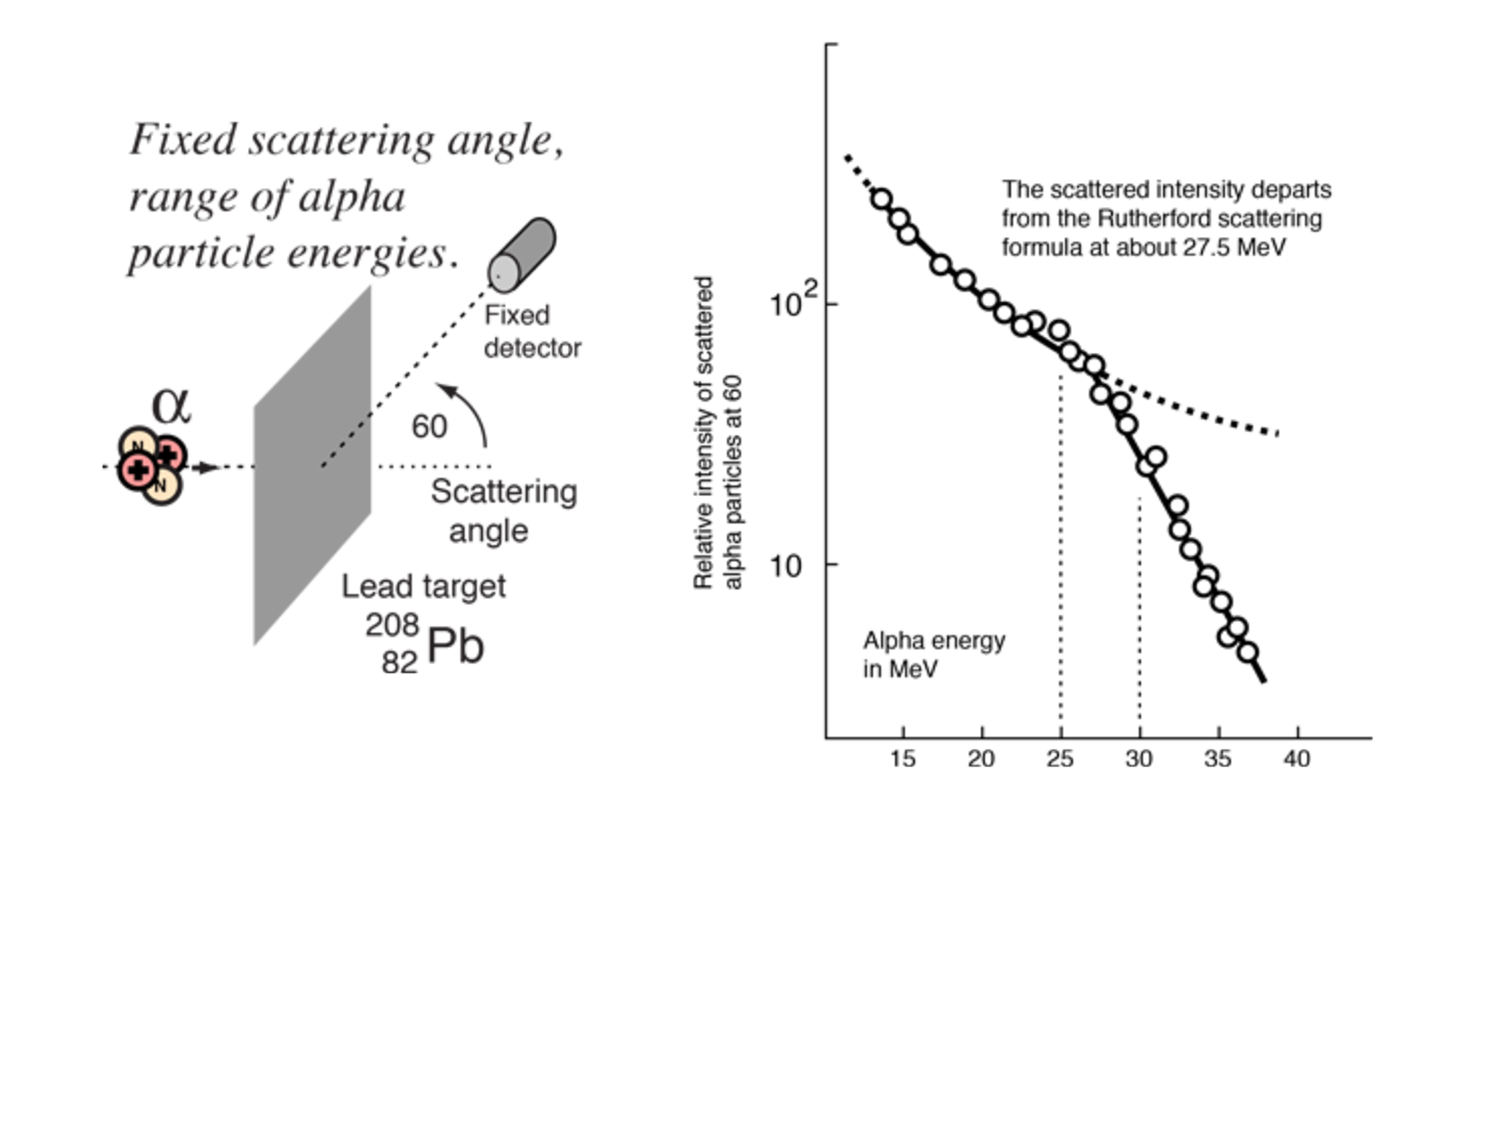
\includegraphics[scale=0.5]{/errore_ruth}
\caption{Il grafico mostra che oltre una certa energia il modello di Rutherford non funziona più e che subentrano altre interazioni}
\end{figure}
\item Stabilità dell'atomo \\
Se immaginiamo che gli elettroni siano fermi intorno al nucleo, questi dovrebbero cadere sul nucleo sotto l'azione coulombiana, quindi non possono essere fermi ed in tal caso l'intero atomo avrebbe le dimensioni del nucleo, e non è così.
Allora si può pensare agli elettroni orbitanti intorno al nucleo, ma siccome sono cariche accelerate dovrebbero emettere energia sotto forma di onde elettromagnetiche e perderebbero energia al punto da cadere sul nucleo: di nuovo l'atomo dovrebbe coincidere con le dimensioni del nucleo.
\item Spettro atomico discreto \\
Gli elettroni dovrebbero irradiare energia sotto forma di onde elettromagnetiche con uno spetto continuo della radiazione emessa, ma ciò che si osserva negli esperimenti che sono spettri atomici discreti.
\end{enumerate}


\subsection{Spettri atomici} 
Quando si parla di spettro atomico si fa riferimento all'emissione elettromagnetica discreta di un gas monoatomico.
Gli spetti atomici possono essere osservati utilizzando una scarica elettrica passante attraverso una regione contenete il gas.
A causa della scarica, e della collisione tra atomi, gli elettroni di alcuni degli atomi si pongono in uno stato energetico in cui la loro energia totale è maggiore di quella di un atomo non eccitato.
Tornando poi ad uno stato energetico inferiore, l'eccesso di energia si manifesta attraverso l'emissione di radiazione elettromagnetica: un fotone.
Essa viene poi collimata da una fessura (diaframma) e fatta passare attraverso un prisma, è possibile allora osservare sulla lastra fotografica uno spettro discreto.
Ogni tipo di atomo ha un suo spettro caratteristico, quindi lunghezze d'onda ben precise.
\begin{figure}[h]
\centering
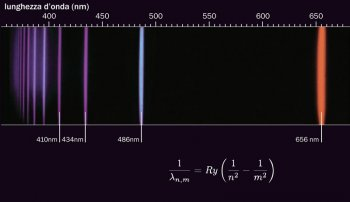
\includegraphics[scale=1]{/INFN_Asimmetrie22_pag8_img1}
\caption{Le righe spettrali emesse nel visibile dall’atomo di idrogeno. Le prime quattro da destra furono osservate inizialmente da Ångström. I valori osservati vengono riprodotti dalla formula di Rydberg-Balmer fissando Ry=10.9721 cm-1 e n=2, per m=3,4,5,6.}
\end{figure}
Nel 1885 \textit{Johann J. Balmer} osservò alcune righe dello spettro di emissione dell'idrogeno che possono essere calcolate utilizzando la \underline{formula di Balmer}:
\begin{equation}
\lambda = 3646 \frac{n^2}{n^2 - 4} \quad \mbox{ (in $\AA$}
\end{equation}
Righe di emissione dell'idrogeno:
\begin{itemize}
\item $H_{\alpha}$ $n=3$ $\rightarrow$ red $\lambda = \SI{6562.8}{\AA}$
\item $H_{\beta}$ $n=4$ $\rightarrow$ blue $\lambda = \SI{4861.3}{\AA}$
\item $H_{\gamma}$ $n=5$ $\rightarrow$ violet $\lambda = \SI{4340.5}{\AA}$
\end{itemize}
Balmer suppose che tale formula fosse, in realtà, un caso particolare di una legge più generale.
Infatti tale formula venne trovata da \textit{Johannes Rydberg} e \textit{Walther Ritz}, sempre relativa all'idrogeno,
ovvero la \underline{formula di Ridberg} (1908)
\begin{equation}
\begin{split}
& k = \frac{1}{\lambda} = R_H \biggl( \frac{1}{n_1^2} - \frac{1}{n_2^2}  \biggr) \\
& \mbox{con } n_{1} \mbox{, } n_{2} \in \mathbb{N} > 0 : n_{1} < n_{2} \\
& R_H = \SI{10967757.6}{m^{-1}} \quad R \mbox{ dell'idrogeno}
\label{formula_Ridberg}
\end{split}
\end{equation}
Ed infine trovarono la \underline{formula di Ridberg-Ritz} (1908) per gli elementi alcalini
\begin{equation}
k = \frac{1}{\lambda} = R \biggl[ \frac{1}{(m-a)^2} - \frac{1}{(n-b)^2}  \biggr]
\end{equation}
Dove $a, b$ sono fissi per una data serie, $m$ è un intero fisso e $n$ è un intero variabile.
Si scoprirono altre serie di linee come mostrato in figura \ref{serie_linee} e che per tutti gli elementi alcalini le formule associate hanno tutte la stessa struttura.
\begin{figure}[h]
\centering
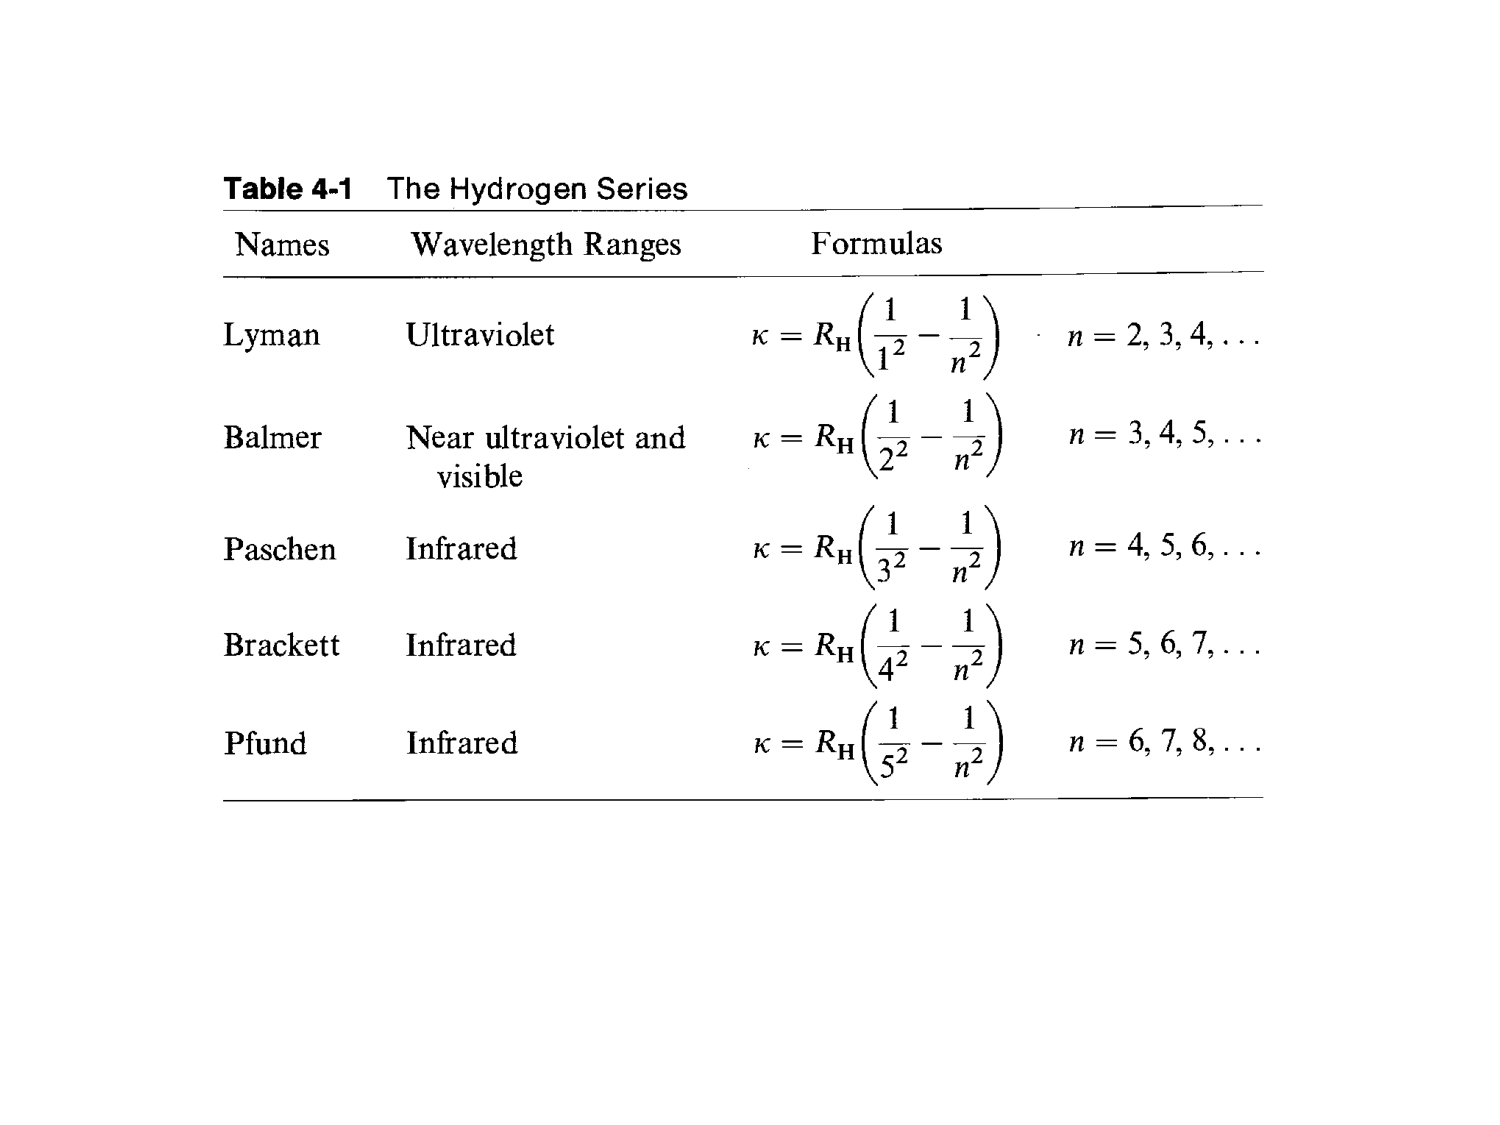
\includegraphics[scale=0.6]{/serie_linee_idrogeno}
\caption{CAPTION}
\label{serie_linee}
\end{figure}
Questo fatto che lo spettro fosse discreto e non continuo era inspiegabile con i modelli atomici di Thomson e Rutherford. 
Occorre sapere che per ogni riga dello spettro di emissione ce n'è una nello spettro di assorbimento.
\begin{figure}[h]
\centering
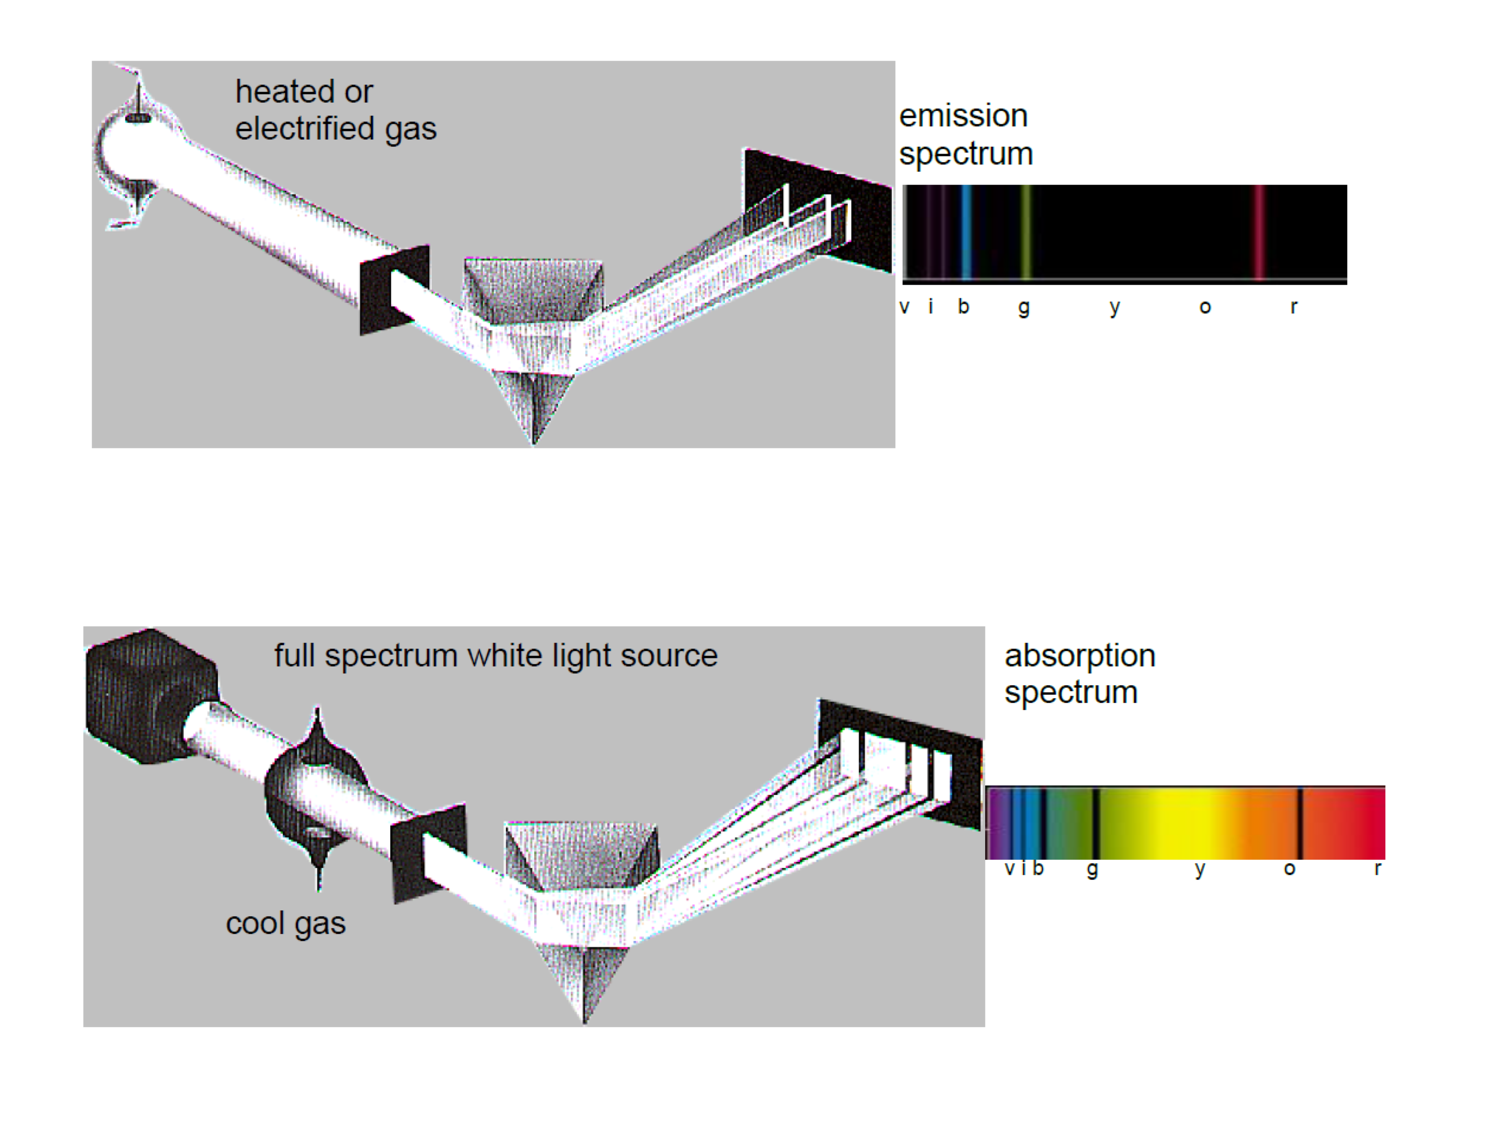
\includegraphics[scale=0.5]{/linee_assorbimento_emissione}
\caption{Oltre allo spetto di emissione si studia anche lo spettro di assorbimento}
\end{figure}


\subsection{Modello di Bohr (1913)}
Entrambi i modelli precedenti (di Thompson e di Rutherford) non riescono però a spiegare l'emissione e l'assorbimento degli spettri atomici prodotti da elementi gassosi.
Il modello di Rutherford inoltre presentava molti problemi di stabilità dell'atomo stesso, come visto in precedenza.
Bohr costruisce un modello atomico sulla base dei risultati degli esperimenti di spettroscopia sull'idrogeno, fondandolo su quattro \underline{postulati}:
\begin{enumerate}
\item Un elettrone si muove su un'orbita \textbf{circolare} attorno al nucleo, soggetto a una attrazione Coulombiana.
\item Non tutte le orbite sono permesse, ma solo quelle tali che $L=n\hbar$, con $n=1, 2, 3, ... $. Introduce una regola di quantizzazione per il momento angolare dell'elettrone.
\item L'elettrone che si muove sulle orbite permesse non produce emissione elettromagnetica, la sua energia totale non varia (viene rimosso il problema della stabilità dell'atomo)
\item Viene emessa radiazione elettromagnetica, di frequenza $\nu$, quando un elettrone passa da un' orbita permessa ad un'altra; tale frequenza è data da $ \nu = \frac{(E_i - E_f)}{h}$
\end{enumerate}

\paragraph{Atomo di idrogeno} Consideriamo un atomo con un nucleo di carica $Ze$ e massa $M$ ed un solo elettrone di carica $e$ e massa $m$, quindi un atomo di idrogeno, ed assumiamo inizialmente che $m \ll M$ approssimando così il nucleo fisso nello spazio e l'elettrone orbitante attorno ad esso.
Impostiamo la condizione di stabilità meccanica dell'elettrone, dove compare la forza di attrazione coulombiana tra nucleo ed elettrone che viene compensata dalla forza centrifuga
\begin{equation}
\begin{split}
F_{coulomb} & = ma_{centrifuga} \\ 
\frac{1}{4\pi \varepsilon_0} \frac{Z e^2}{r^2} & = m \frac{v^2}{r}
\end{split}
\end{equation}
Il momento angolare $L$ è 
\begin{equation}
\begin{split}
L & = m v r = n \hbar \\
v & = \frac{ n\hbar}{m r }
\end{split}
\end{equation}
da cui ottengo 
\begin{equation}
Ze^2 = 4 \pi \varepsilon_0 m v^2 r = 4\pi \varepsilon_0 m r \Bigl(  \frac{ n\hbar}{mr }  \Bigr)^2 = 4\pi \varepsilon_0 \frac{ n^2 \hbar^2}{m r }
\end{equation}
e trovo il raggio dell'orbita
\begin{equation}
\begin{split}
& r = 4\pi \varepsilon_0 \frac{ \hbar^2 n^2}{m Z e^2 } \quad\Rightarrow\quad r \propto \frac{ n^2}{Z }\\
& \mbox{in cui} \quad n = 1,2,3,...
\label{raggio_bohr}
\end{split}
\end{equation}
Da questa relazione vedo in modo esplicito la quantizzazione dell'orbita: il raggio dell'orbita dipende dal quadrato del numero $n$.
Da questa espressione posso trovare inoltre la velocità
\begin{equation}
v = \frac{ n\hbar}{m r } = \frac{ 1}{4\pi \varepsilon_0 } \frac{ Z e^2}{n\hbar } \quad\Rightarrow\quad v \propto \frac{ Z}{n }
\label{velocita_bohr}
\end{equation}
Per $n=1$ ottengo i valori
\begin{equation}
\begin{split}
& r = \SI{5.3e-11}{m} \simeq \SI{0.5}{\AA} \\
& v = \SI{2.2e6}{m/s} \simeq 1\% c
\end{split}
\end{equation}
Il modello di Bohr è costruito sull'atomo di idrogeno, per cui funziona benissimo per l'idrogeno e bene per atomi leggeri (come l'elio ionizzato), con numero atomico piccolo, ma non funziona per atomi più pesanti.
La quantizzazione del momento angolare implica l'esistenza di orbite permesse.
\paragraph{Energia totale} Calcoliamo l'energia totale di un elettrone nelle orbite permesse, utilizzando le relazioni per il raggio \ref{raggio_bohr} e per la velocità \ref{velocita_bohr}, sarà data dall'energia cinetica più l'energia potenziale, che sono rispettivamente $K$ e $V$
\begin{equation}
\begin{split}
K & = \frac{ 1}{2 } m v^2 = \frac{ 1}{2 } m \Bigl[ \frac{ Z e^2}{4\pi \varepsilon_0 \hbar n } \Bigr]^2 = \frac{ 1}{2 } \frac{ m Z^2 e^4 }{(4\pi \varepsilon_0)^2 \hbar^2 n^2 } \\
V & = - \frac{ Z e^2}{4 \pi \varepsilon_0 r } = - \frac{ Z e^2}{4\pi \varepsilon_0 } \Bigl[ \frac{ m Z e^2}{4\pi \varepsilon_0 \hbar^2 n^2 } \Bigr]^2 = - \frac{ m Z^2 e^4}{(4\pi \varepsilon_0)^2 \hbar^2 n^2 }
\end{split}
\end{equation}
la cui somma equivale a
\begin{equation}
\begin{split}
E = K + V = - \frac{ 1}{2 } \frac{ m Z^2 e^4 }{(4\pi \varepsilon_0)^2 \hbar^2 n^2 } = - K
\end{split}
\end{equation}
Inserendo il valore di $r$ ricavato sopra troviamo una relazione importante
\begin{equation}
E = - \frac{ m e^4}{2 (4\pi \varepsilon_0)^2 \hbar^2 } \frac{ Z^2}{n^2 } \quad\Rightarrow\quad E \propto \frac{ Z^2}{n^2 }
\label{energia_quantizzata}
\end{equation}
dove $n=1,2,3,...$ è il numero quantico.
Quindi la quantizzazione del momento angolare non solo implica che solo alcune orbite sono permesse ma implica anche la quantizzazione dell'energia, vedi figura \ref{energie_permesse}.
L'energia più negativa lo ho per $n=1$, quindi lo stato di energia più basso è lo stato più stabile: tutti i sistemi fisici tendono ad andare verso il minimo dell'energia, tale stato è detto \underline{stato fondamentale} (o \textit{ground state})
tale che per $n=1$ e $Z=1$ l'energia dello stato fondamentale è
\begin{equation}
E_{min} = -\SI{2.179868e-18}{J} = - \SI{13.6}{eV}
\label{energia_fondamentale}
\end{equation}
\begin{figure}[h]
\centering
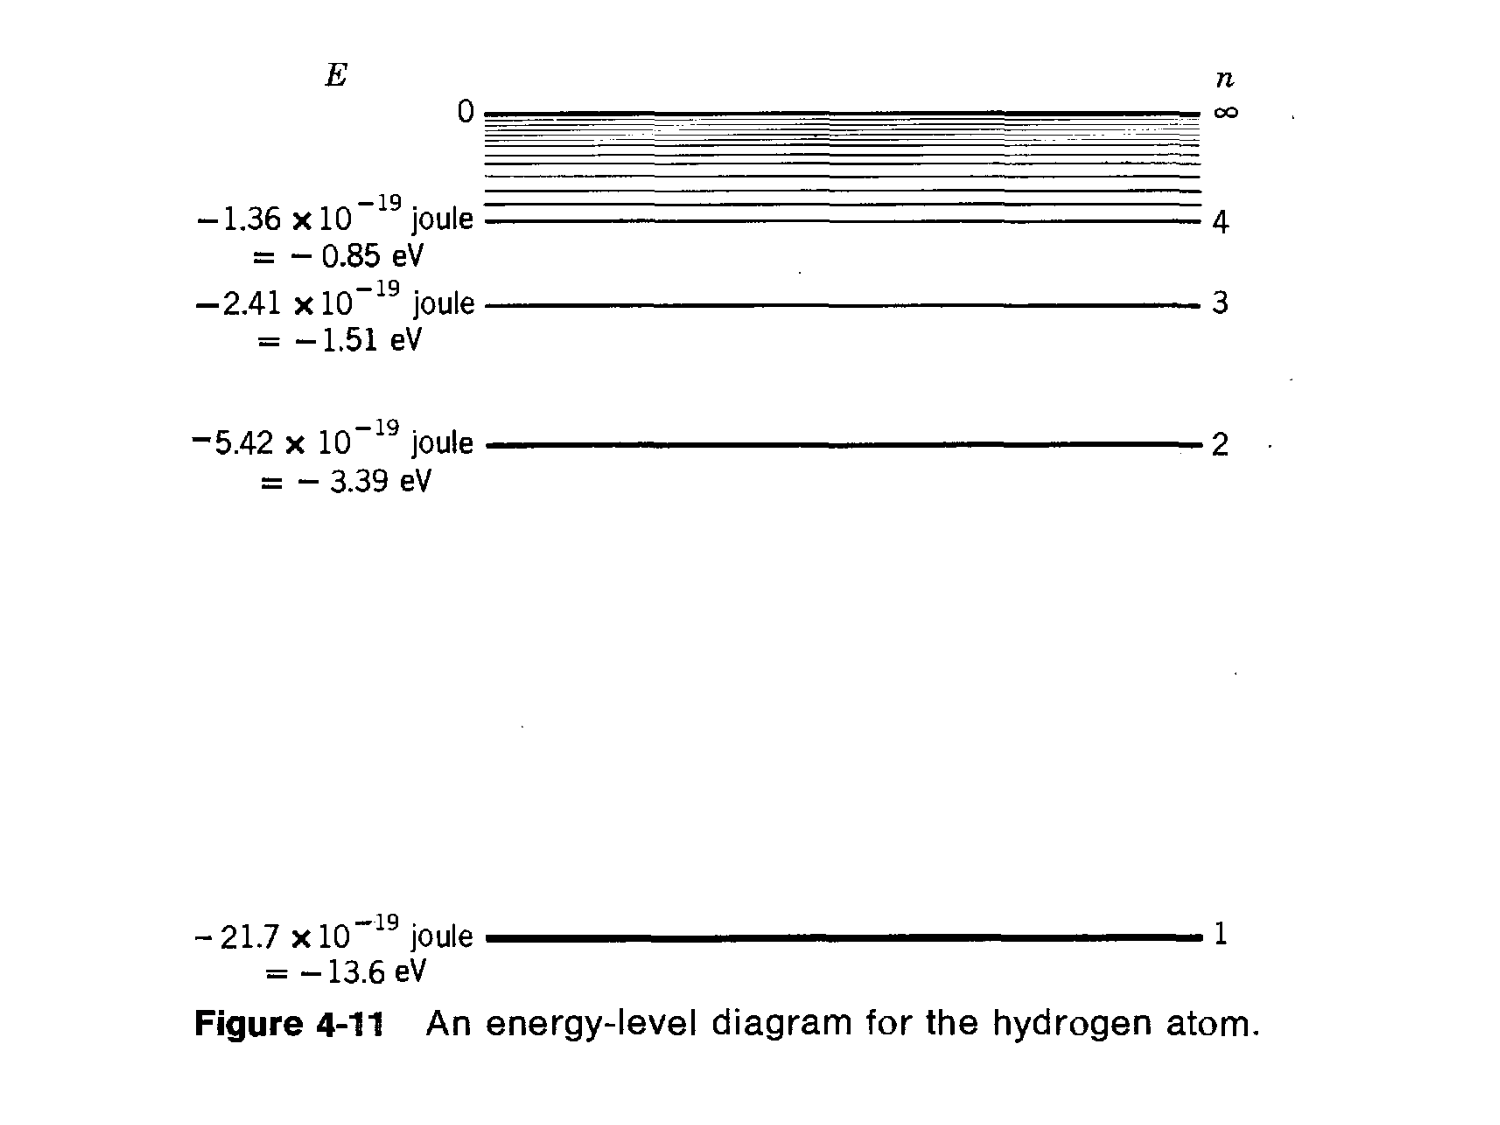
\includegraphics[scale=0.4]{/livelli_energia}
\caption{Diagramma delle energie permesse nell'atomo di idrogeno}
\label{energie_permesse}
\end{figure}

\paragraph{Modello di Bohr vs spettri atomici}
Utilizzando la formula \ref{energia_quantizzata} per le energie permesse ed applichiamo il quarto postulato di Bohr per calcolare la frequenza della radiazione emessa nel passaggio tra uno stato iniziale $E_i$ ed uno stato finale $E_f$ di energia
\begin{equation}
\nu = \frac{ E_f - E_i}{h } = \Bigl(  \frac{ 1}{4 \pi \varepsilon_0 }  \Bigr)^2 \frac{ m Z^2 e^4}{4\pi \hbar^3 } \Bigl(  \frac{ 1}{n_f^2 } - \frac{ 1}{n_i^2 }  \Bigr)
\end{equation}
In termini di lunghezza d'onda reciproca, che compare nella formula di Ridberg \ref{formula_Ridberg}
\begin{equation}
\begin{split}
& k = \frac{ 1}{\lambda } = \frac{ \nu}{c } \\
& k = \Bigl(  \frac{ 1}{4 \pi \varepsilon_0 }  \Bigr)^2 \frac{ m Z^2 e^4}{4\pi \hbar^3 c} \Bigl(  \frac{ 1}{n_f^2 } - \frac{ 1}{n_i^2 }  \Bigr) \\
& k = R_{\infty} Z^2 \Bigl(  \frac{ 1}{n_f^2 } - \frac{ 1}{n_i^2 }  \Bigr) \\
& \mbox{con la costante} \quad R_{\infty} = \Bigl(  \frac{ 1}{4 \pi \varepsilon_0 }  \Bigr)^2 \frac{ m Z^2 e^4}{4\pi \hbar^3 c} = \SI{109737}{cm^{-1}}
\end{split}
\end{equation}
Dove $R_{\infty}$ risulta un po' più grande della costante di Ridberg $R_H$ per l'idrogeno.
Tale formula restituisce tutti i valori di $k$ del set di linee che costituiscono lo spettro atomico, con il vincolo sui numeri $n_i, n_f \in \mathbb{N} \quad t.c \quad n_i > n_f$.
Il modello di Bohr spiega anche lo spettro di assorbimento: i fotoni assorbiti sono solo quelli che permettono agli elettroni di saltare ad uno stato con energia maggiore, per cui solo a determinate frequenze.
Nello spettro di assorbimento possono avvenire solo quei processi per cui da $n=1$ si passa a orbite di energia maggiore ovvero con $n>1$ ed è per questo che potremo vedere in assorbimento solo la serie di Lyman;
ciò è dovuto al fatto che il gas si trova inizialmente allo stato fondamentale, solo se fosse inizialmente in uno stato eccitato allora si vedrebbero ulteriori serie in assorbimento (Balmer, Paschen).
\begin{figure}[h]
\centering
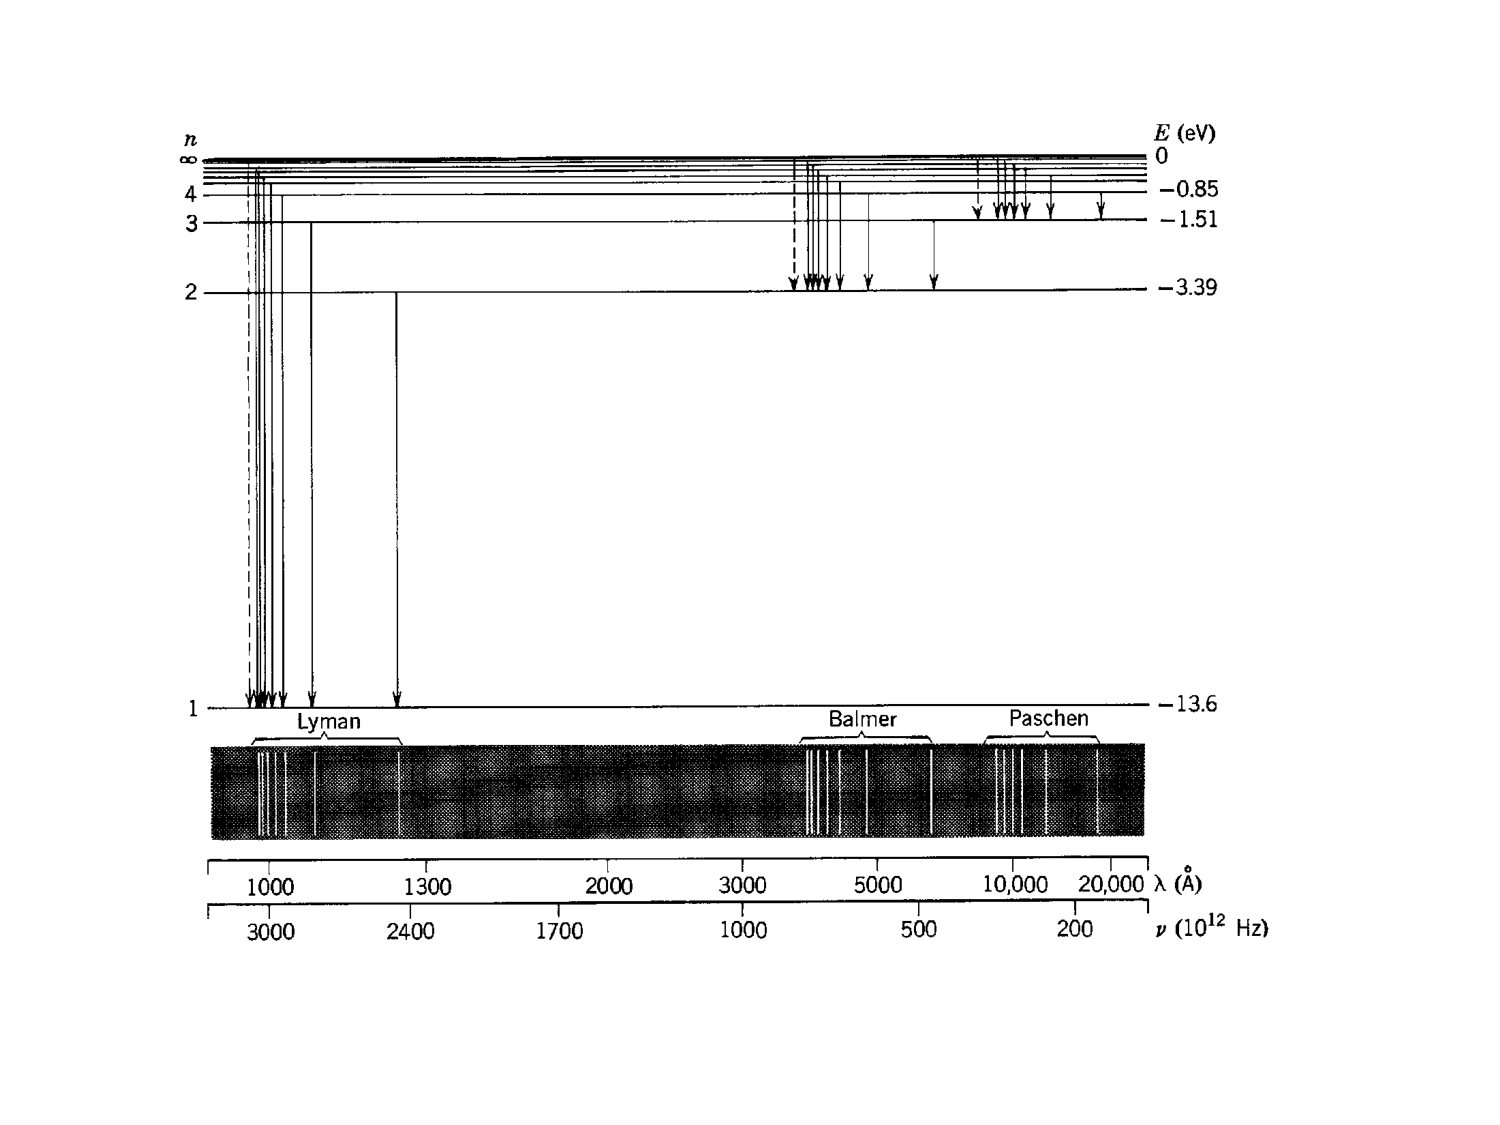
\includegraphics[scale=0.5]{/spettro_atomico_idrogeno}
\caption{La serie di Lyman è costituita da tutte le transizioni da un qualsiasi stato $n_i$ ad uno stato $n_f = 1$.
La serie di Balmer è costituita da tutte le transizioni da un qualsiasi stato $n_i$ ad uno stato $n_f = 2$.
Analogamente per le altre serie.
Nel transire da orbite superiori ad orbite inferiori l'elettrone perde energia emessa sotto forma di radiazione elettromagnetica.}
\end{figure}

\paragraph{Correzione massa ridotta} Nei conti precedenti si era approssimato il nucleo fisso nello spazio, se invece si considerano nucleo ed elettrone entrambi orbitanti intorno al centro di massa si deve utilizzare la massa ridotta
\begin{equation}
\mu = \frac{ m M}{m + M }
\end{equation}
e questa correzione si applica anche alla costante di Ridberg
\begin{equation}
R_H^{teorico} = \frac{ \mu}{ m} R_{\infty}^{teorico}
\end{equation}
In cui è facile vedere che 
\begin{equation}
\begin{split}
& \frac{ \mu}{m } = \frac{ 1}{1 + \frac{ m}{M } } \\
& \mbox{se}\quad M \gg m  \Rightarrow \frac{ m}{M } \to 0 \\
& \frac{ \mu}{m }\to 1 \Rightarrow R_H \to R_{\infty}
\end{split}
\end{equation}
I valori della costante di Ridberg sono
\begin{equation}
\begin{split}
R_{\infty}^{teorico} & = \SI{109737}{cm^{-1}} \\
R_{H}^{teorico} & = \SI{109681}{cm^{-1}} \\
R_{H}^{sperim} & = \SI{109678}{cm^{-1}}
\end{split}
\end{equation}
con questa correzione il valore su $R_H$ teorico si avvicina notevolmente al valore sperimentale.


\subsection{Esperimento di Franck-Hertz}
Il setup sperimentale, vedi figura \ref{esp_Franck_Hertz_a}, prevede un'ampolla con atomi di mercurio in cui si trova un filamento riscaldato che emette elettroni, una differenza di potenziale tra due piastre per accelerarli e farli passare attraverso una griglia carica positivamente.
\paragraph{La prima parte dell'esperimento}
Consiste nell'aumentare gradualmente il voltaggio accelerante, quindi l'energia degli elettroni, e per ogni valore misurare la corrente elettrica con un amperometro, vedi figura \ref{esp_Franck_Hertz_b},.
Si accorsero che in corrispondenza dei minimi, a $\SI{4.89}{V}$, $\SI{6.67}{V}$, $\SI{8.84}{V}$, $\SI{9.80}{V}$, gli elettroni non raggiungono il piatto collettore.
La spiegazione che diedero è che con energie minori di $\SI{4.0}{eV}$ l'elettrone urta contro l'atomo di mercurio senza perdere energia, mentre quando l'energia aumenta, ad esempio a $\SI{4.9}{eV}$, l'elettrone perde tutta la sua energia non potendo più raggiungere l'altro elettrodo; quando l'energia supera ad esempio $\SI{6.0}{eV}$ l'elettrone perde parte della sua energia ma ne possiede ancora per arrivare all'altro elettrodo; in corrispondenza degli altri minimi succedono cose analoghe; ed infine per energie vicine a $\SI{10}{eV}$ ipotizzarono una doppia interazione che porta a perdere molta più energia.
Solo gli elettroni che hanno energie precise fanno compiere agli elettroni dell'atomo salti energetici.
\begin{figure}[h]
    \centering
    \subfloat[Strumentazione]{
        \label{esp_Franck_Hertz_a}
        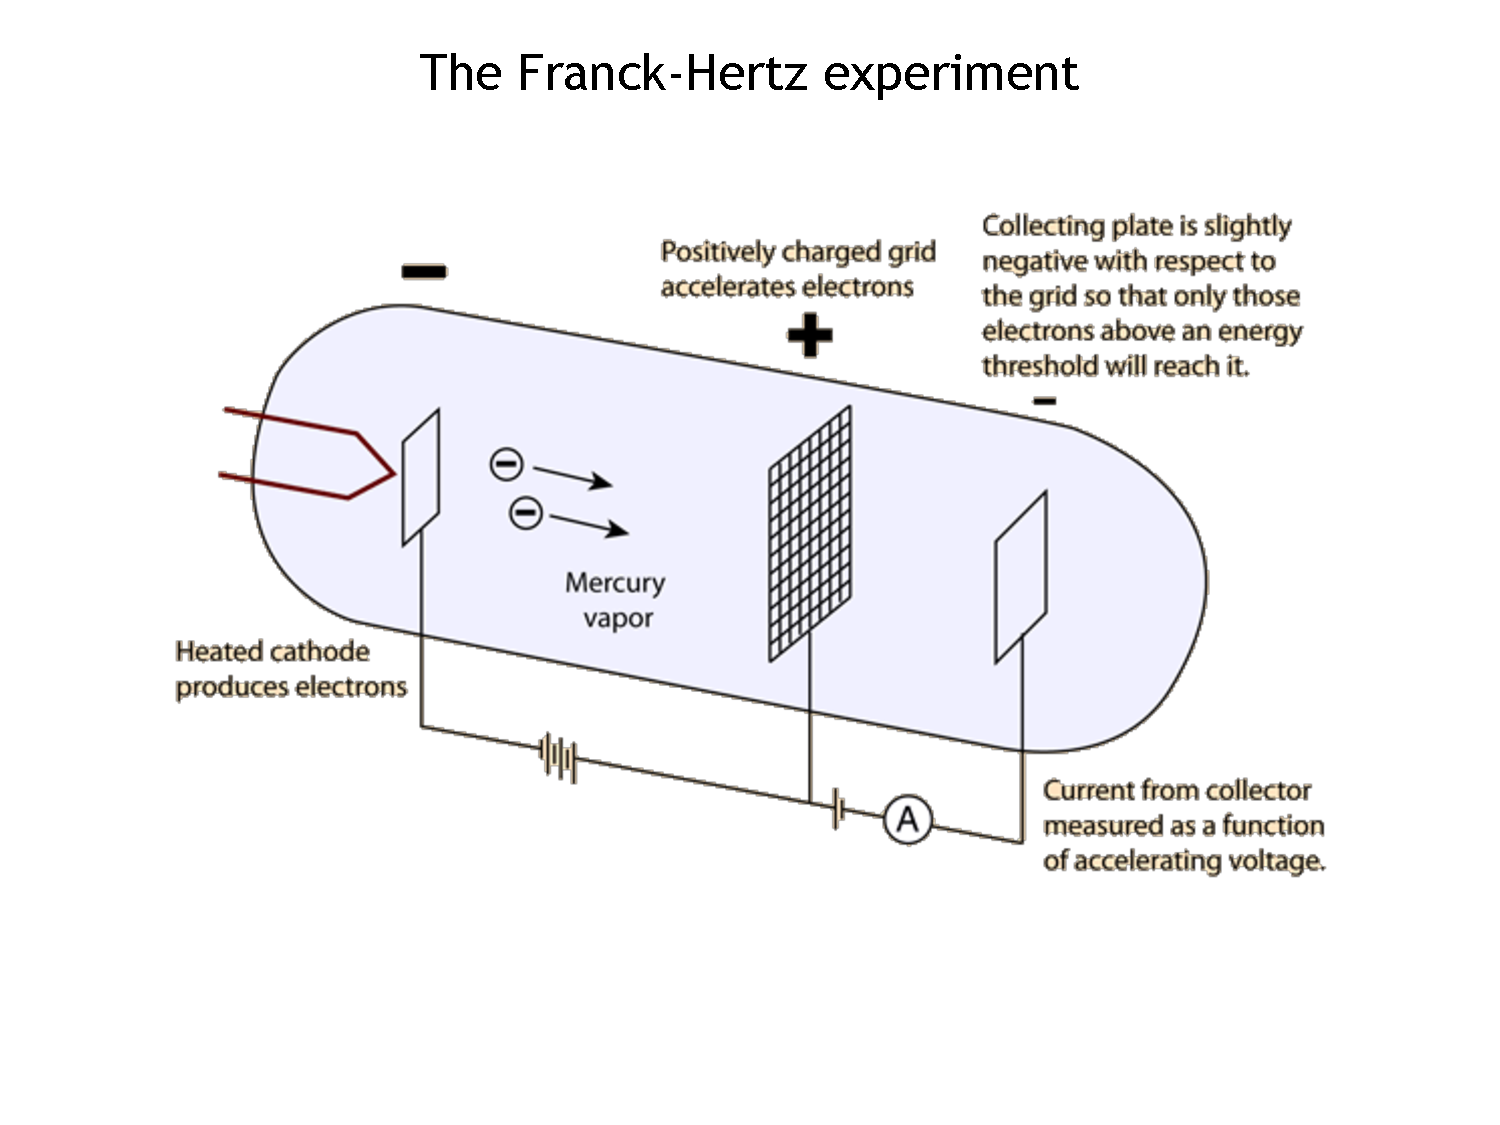
\includegraphics[width=0.5\textwidth]{/esp_Franck_Hertz}
    }
    \subfloat[Dati ottenuti]{
        \label{esp_Franck_Hertz_b}
        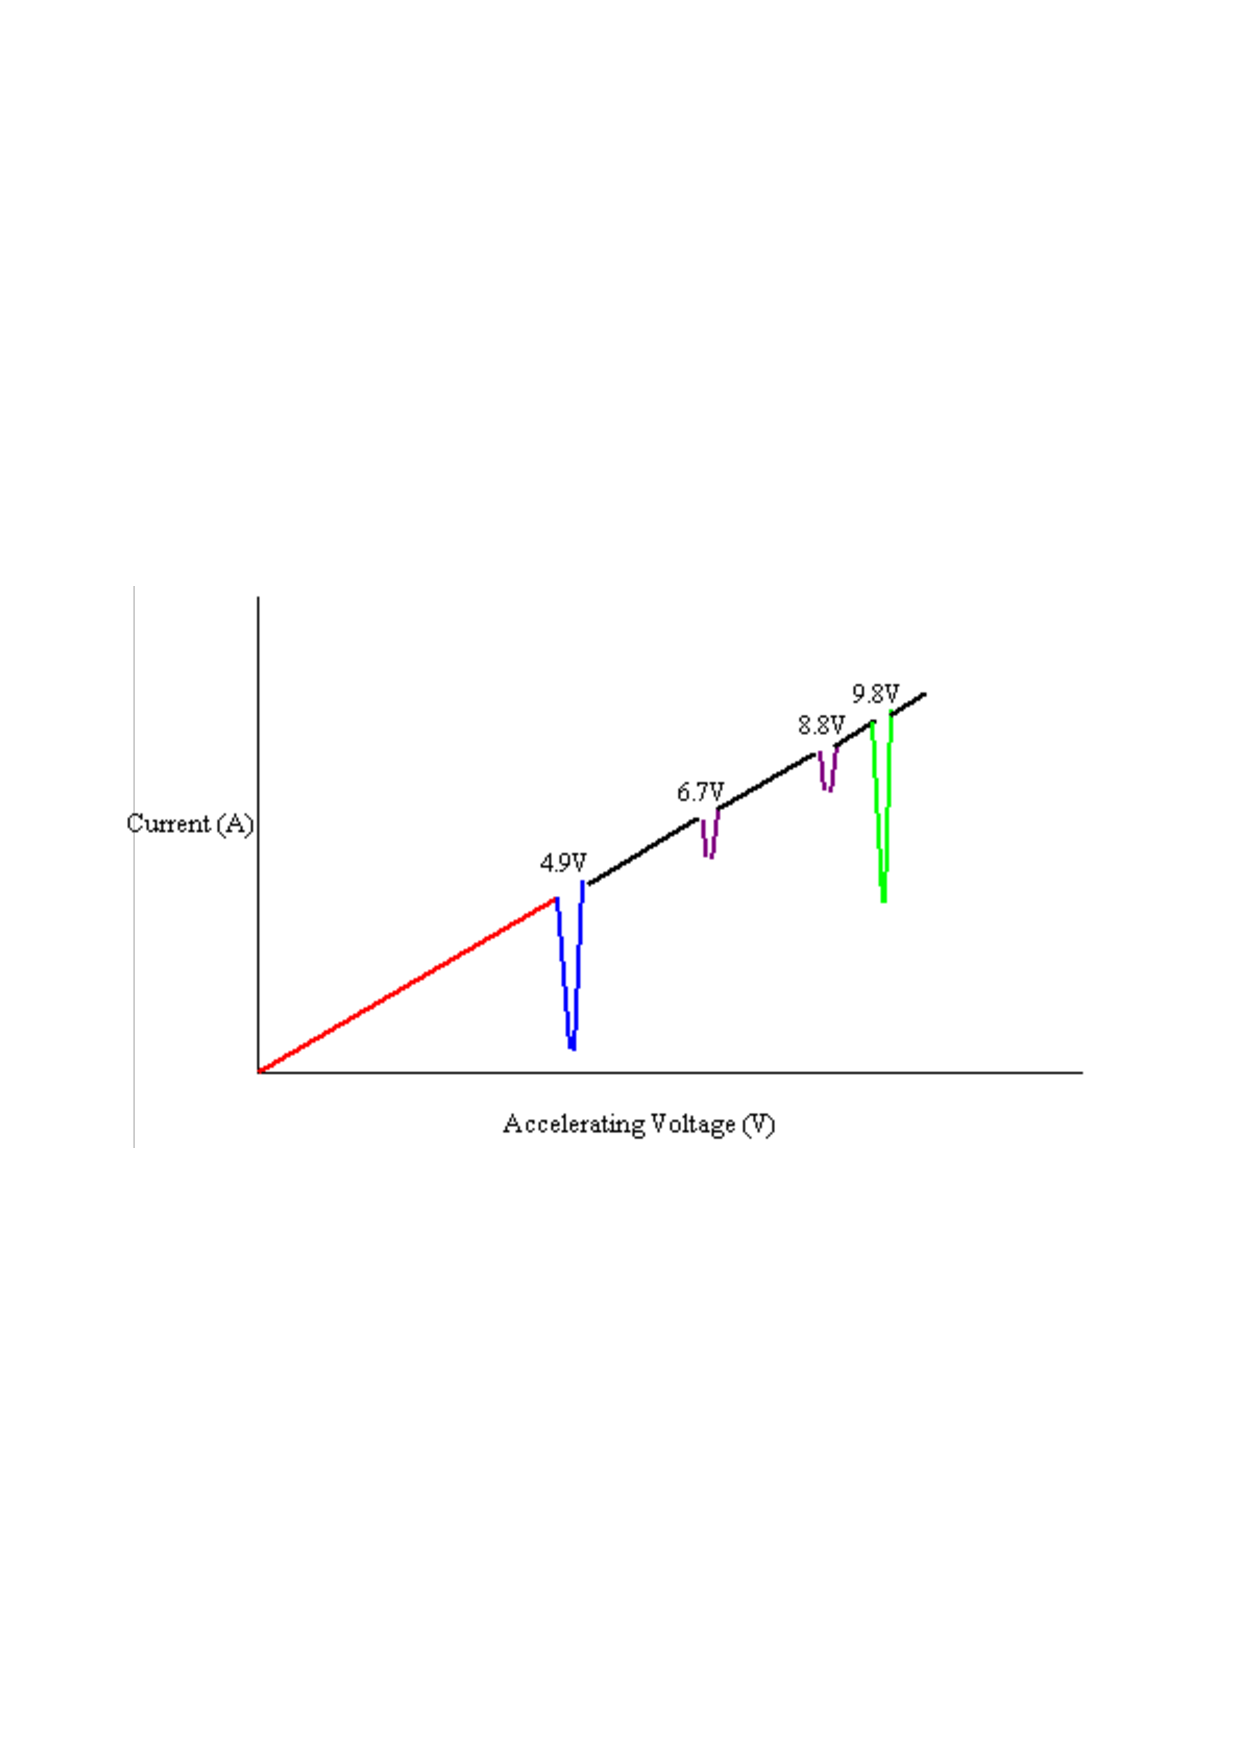
\includegraphics[width=0.5\textwidth]{/ris2_esp_Franck_Hertz}
    }
    \caption{Esperimento di Franck e Hertz}
    \label{esp_Franck_Hertz_overall}
\end{figure}

\paragraph{La seconda parte dell'esperimento} 
Consiste nell'osservare la radiazione emessa dagli atomi di mercurio.
Trovarono una corrispondenza, utilizzando l'equazione $E=h\nu$, tra le energie dei minimi di voltaggio e le frequenze della luce emessa.
Vedi figura \ref{emissione_Hg}.
\begin{figure}[h]
\centering
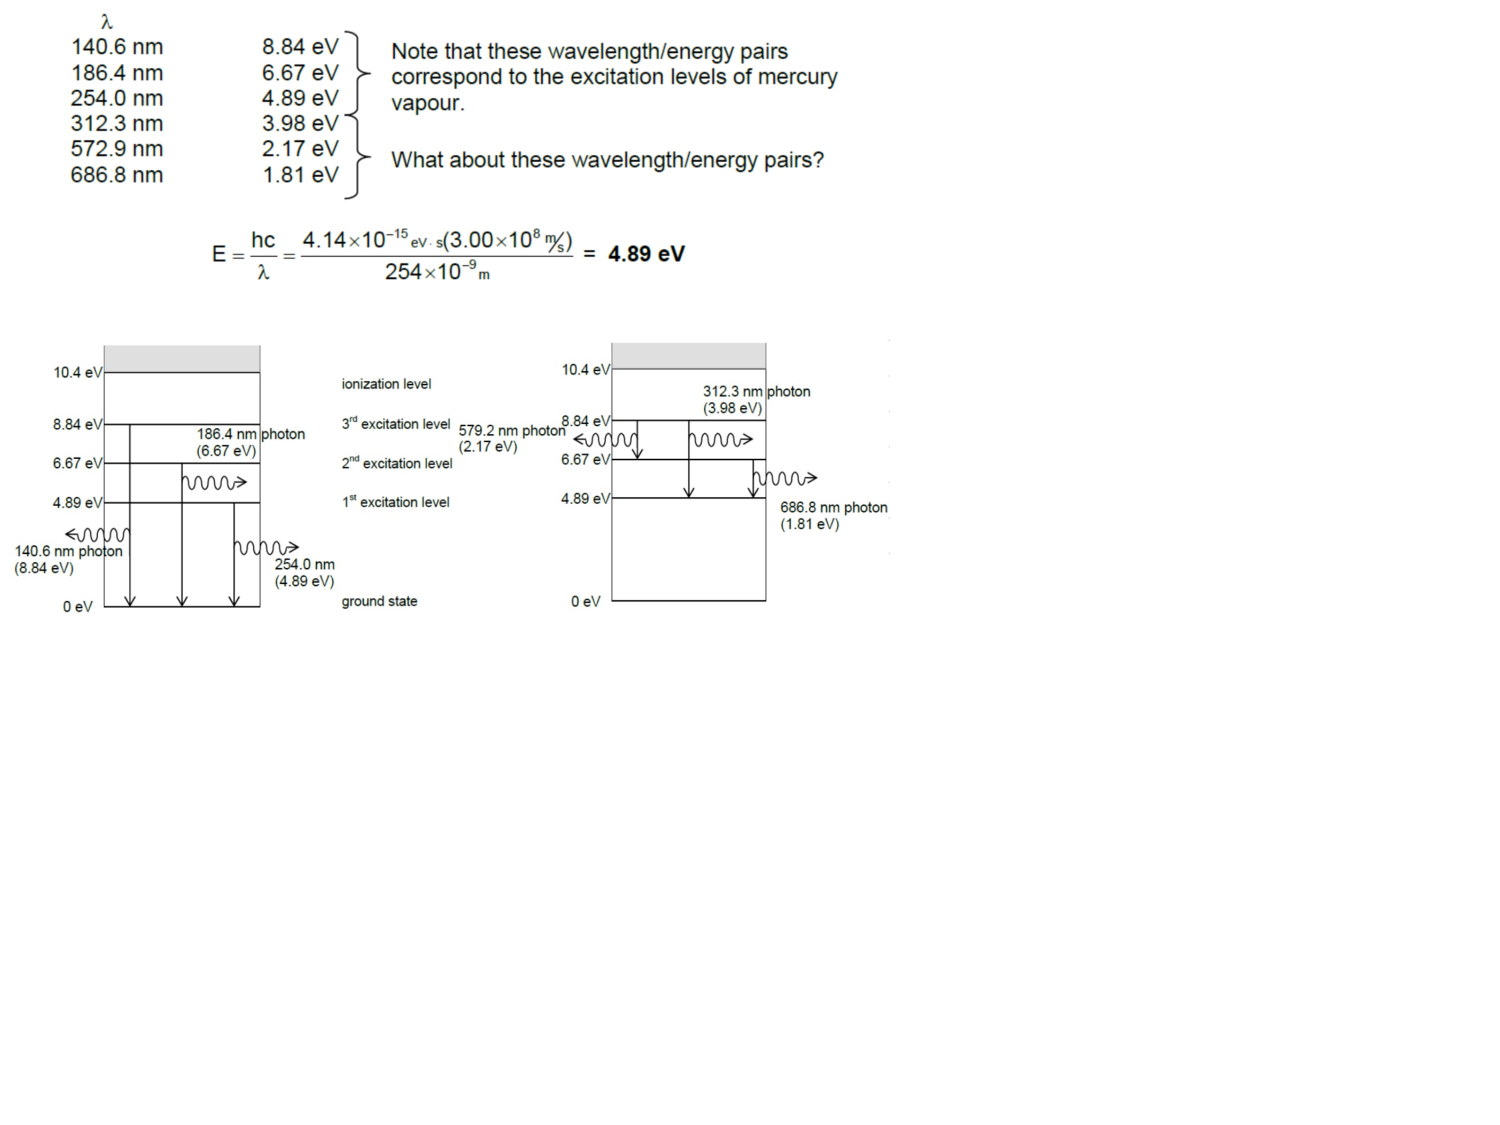
\includegraphics[scale=0.7]{/ionizzazione}
\caption{Livelli di ionizzazione degli elettroni all'interno dell'atomo di mercurio}
\label{emissione_Hg}
\end{figure}


\subsection{Interpretazione di De Broglie}
Interpretazione di De Broglie della regola di quantizzazione di Bohr.
Parte fondamentale della "old quantum theory".
\begin{equation}
\begin{split}
& L = mvr = pr = \frac{ n h }{2 \pi } \quad \mbox{con } n = 1, 2, 3, ... \\
& p = \frac{ h}{\lambda} \\
& \frac{ h r }{\lambda } = \frac{ n h }{2\pi }   \quad\Rightarrow\quad   2\pi r = n \lambda \quad \mbox{con } n = 1, 2, 3, ...
\end{split}
\end{equation}
dove $r$ è la circonferenza dell'orbita.
Questo risultato illustra che le orbite permesse sono quelle tali per cui la circonferenza dell'orbita può contenere un numero intero di lunghezze d'onda di De Broglie.
È un tentativo di De Broglie per unire la sua teoria al postulato di Bohr.
Quindi l'onda che descrive l'elettrone può essere visualizzata come un'onda stazionaria avvolta sull'orbita.
\begin{figure}[h]
\centering
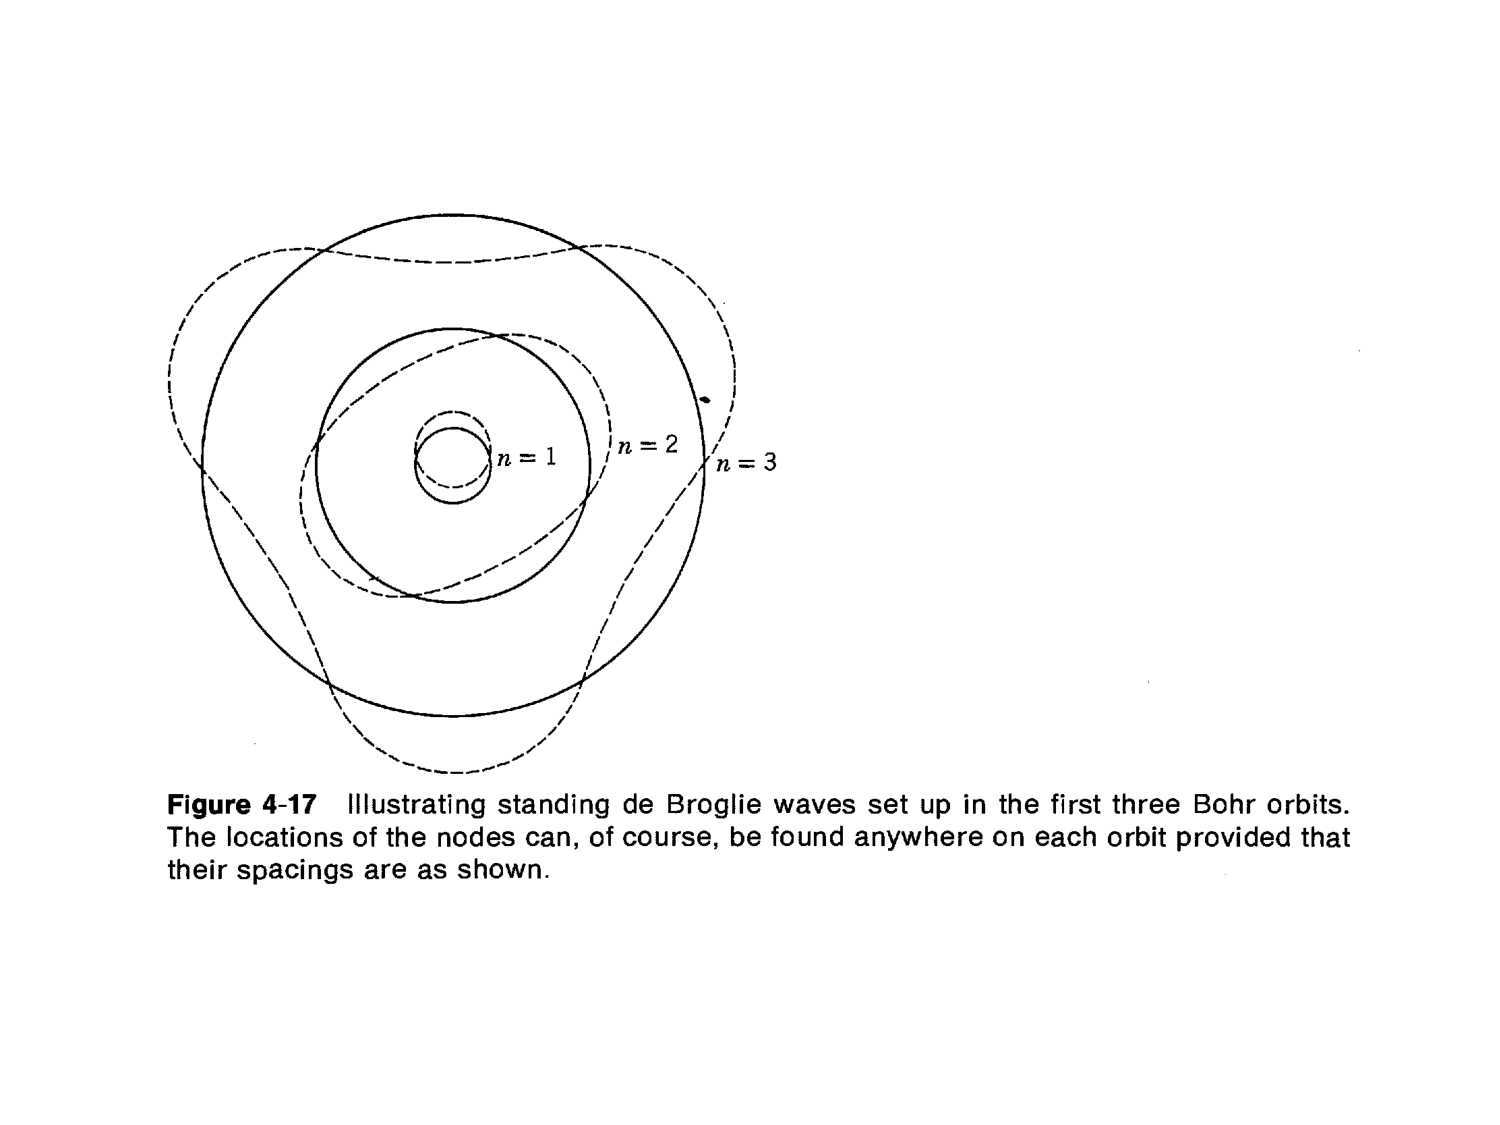
\includegraphics[scale=0.5]{/onda_stazionaria_avvolta}
\caption{Rappresentazione grafica dell'onda-elettrone attorno all'orbita}
\end{figure}


\subsection{Modello di Wilson-Sommerfeld: orbita ellittica}
Sommerfeld sviluppa un modello atomico simile a quello di Bohr ma con importanti differenze.
Questo modello atomico adotta orbite ellittiche e non più circolari come nel modello di Bohr.
Sommerfeld costruì questo modello per riuscire a modellizzare e spiegare una caratteristica degli spettri atomici: la \textit{struttura fine}.
Alcune linee degli spettri atomici sono in realtà composte da più linee, è possibile distinguere ciò a patto che si utilizzi un apparato di misura che abbia una grande precisione.
La distanza tra queste linee che compongono le linee di emissione "grossolane", in termini di lunghezza d'onda, è $\Delta \lambda \sim \SI{e-4}{}$ rispetto alla separazione tra diverse linee.
Quindi vi è uno splitting della linea principale in sotto-linee molto piccolo.
Il modello di Bohr non riesce a spiegare questo fenomeno, motivo per cui Sommerfeld pensa a questo diverso modello.

Sommerfeld applica le sue regole di quantizzazione alla coordinata angolare $\theta$ e alla coordinata radiale $r$
\begin{equation}
\oint L d\theta = n_{\theta} h \quad\quad \quad \oint p_r dr = n_r h
\end{equation}
dalla prima ricava la quantizzazione del momento angolare
\begin{equation}
L = n_{\theta} \hbar \quad\quad n_{\theta} = 1,2,3, ...
\end{equation}
e dalla seconda deriva la condizione
\begin{equation}
L (\frac{ a}{b } - 1) = n_r \hbar \quad\quad n_{r} = 0,1,2,3, ...
\end{equation}
ed usando una relazione di stabilità meccanica, simile a quella utilizzata da Bohr, ottiene le relazioni per i semiassi dell'ellisse $a, b$ e l'energia $E$
\begin{equation}
\begin{split}
& a = \frac{ 4\pi \varepsilon_0 \hbar^2 n^2}{\mu e^2 Z } \quad\quad b = a \frac{ n_{\theta}}{n } \\
& E = - \Bigl(  \frac{ 1}{4\pi\varepsilon_0 }  \Bigr)^2 \frac{ \mu Z^2 e^4}{2 \hbar^2 n^2 }
\end{split}
\end{equation}
dove $\mu$ è la \textit{massa ridotta}, $n_{\theta}$ è il \textit{numero quantico azimutale} e $n$ è il \textit{numero quantico principale} che corrispondono a
\begin{equation}
\begin{split}
n & = n_{\theta} + n_{r} \\
n & = 1,2,3,... \\
n_{\theta} & = 1,2,3,..., n
\end{split}
\end{equation}
La forma dell'orbita risulta quindi essere legata al rapporto tra il semiasse maggiore e minore
\begin{equation}
\frac{ b}{a } = \frac{ n_{\theta}}{n }
\end{equation}
infatti nel caso in cui
\begin{itemize}
\item se $n=1 \Rightarrow n_{\theta}=1$ ho una sola orbita possibile che è circolare
\item se $n=2 \Rightarrow n_{\theta}=1,2$ quindi ho due possibili orbite di cui una circolare e una ellittica
\item se $n=3 \Rightarrow n_{\theta}=1,2,3$ quindi ho tre possibili orbite di cui una circolare e due ellittiche
\end{itemize}
e così via al crescere di $n$.
L'energia dipende solo da $n$, di conseguenza tutte le orbite con stesso $n$ hanno la stessa energia e si dice che queste orbite sono \textit{degeneri}.

Sommerfeld rimosse questo problema di degenerazione delle orbite con una correzione relativistica all'energia totale dell'elettrone:
\begin{equation}
\frac{ v}{ c} \simeq \SI{e-4}{}
\end{equation}
arrivando a dire che queste orbite non hanno la stessa energia e trovando l'energia delle orbite.
Si noti che l'ordine di grandezza di tale correzione è equivalente all'ordine di grandezza dello splitting delle linee dello spettro atomico.
E quindi lo splitting equivale alla radiazione emessa nel passaggio tra orbite \textit{degeneri} con stesso $n$, con energie simili.
La relazione per l'energia con la correzione relativistica trovata da Sommerfeld è
\begin{equation}
\begin{split}
& E = - \frac{ \mu Z^2 e^4}{2 (4\pi\varepsilon_0)^2 \hbar^2 n^2 } \Bigl[ 1 + \frac{ \alpha^2 Z^2}{n } \Bigl(  \frac{ 1}{n_{\theta} - \frac{ 3}{4 n } }  \Bigr) \Bigr] \\
& \alpha = \frac{ 1}{4\pi\varepsilon_0 } \frac{ e^2}{\hbar c } \simeq \frac{ 1}{137 } = \SI{7.297e-3}{} \quad \mbox{Costante di struttura fine}
\end{split}
\end{equation}
introducendo la \textit{costante di struttura fine} $\alpha$.
\begin{figure}[h]
\centering
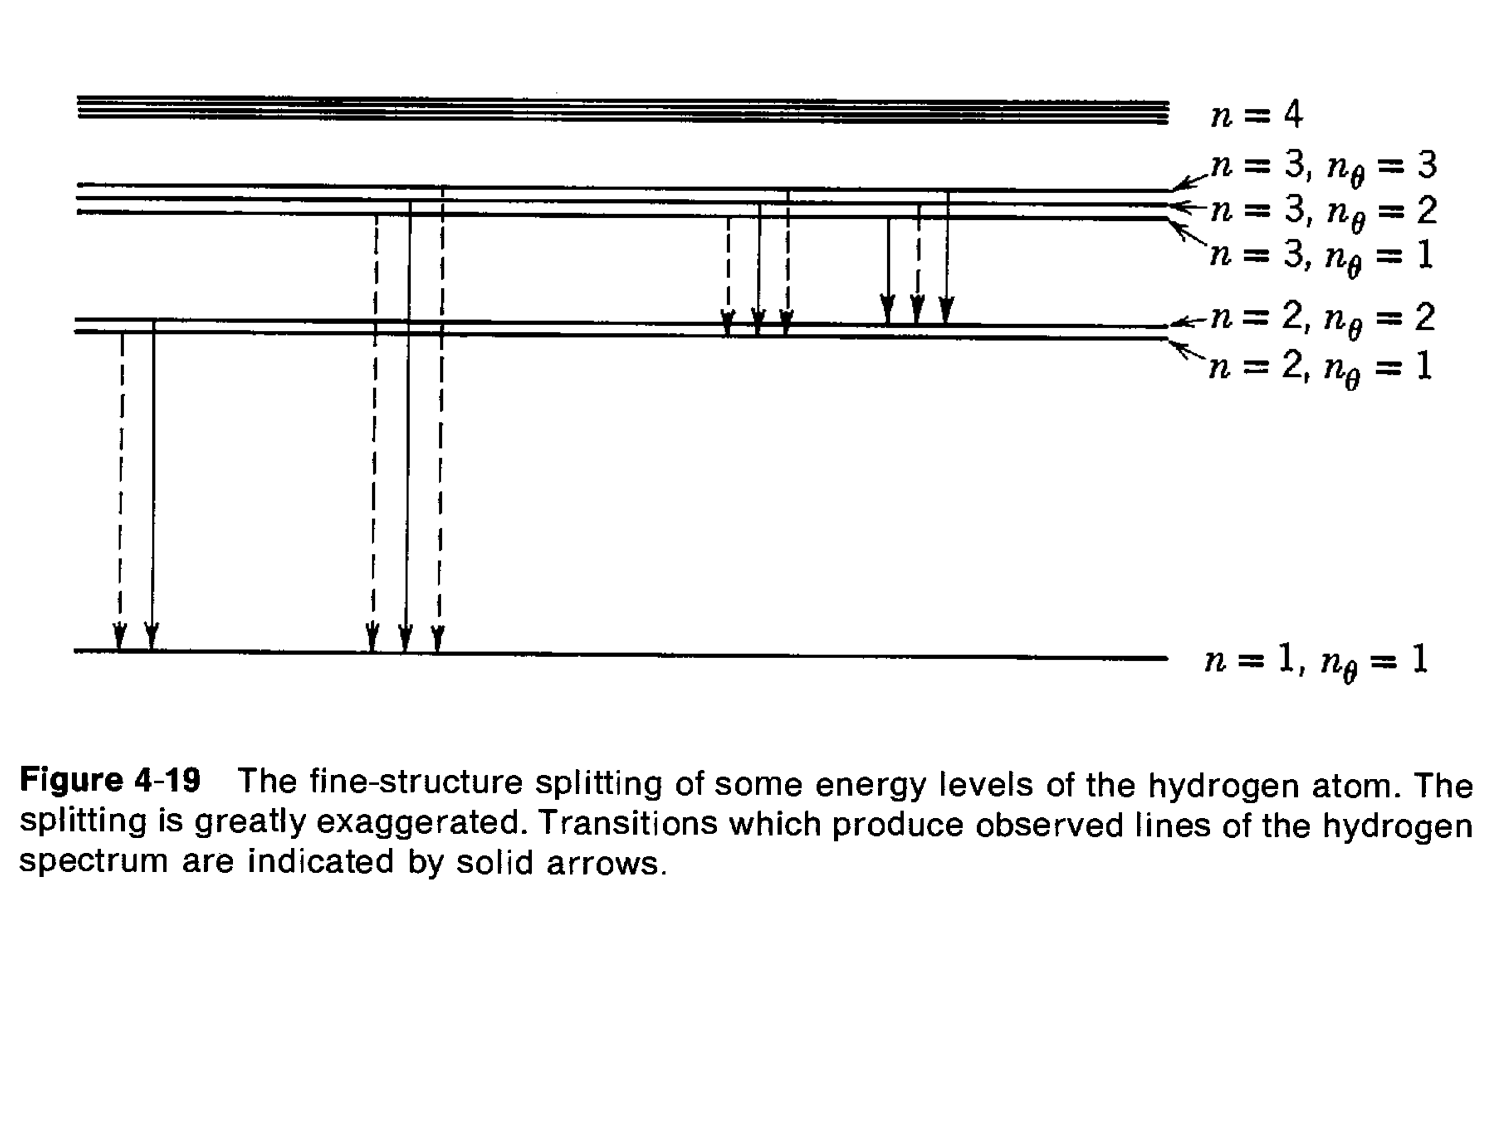
\includegraphics[scale=0.4]{/livelli_energ_sommerfeld}
\caption{Ogni livello energetico viene splittato in più livelli energetici molto vicini fra loro, a seconda del valore del numero quantico $n$. Le transizioni indicate con una linea tratteggiata non sono possibili.}
\end{figure}

\paragraph{Regola di selezione} non tutte le transizioni sono permesse: solo le transizioni per cui è soddisfatta la regola di selezione sono possibili
\begin{equation}
n_{\theta_i} - n_{\theta_f} = \pm 1
\end{equation}

\paragraph{Conclusioni} Il \textbf{modello di Sommerfeld} funziona molto bene ed ebbe un notevole successo, è però basato su una considerazione non corretta: la struttura fine non è conseguenza della correzione relativistica ma è conseguenza dell'interazione \textit{spin-orbita} (vedi corso di Struttura della Materia 2).
A Sommerfeld va attribuito il fatto di aver intuito che fosse necessario rimuovere la degenerazione delle orbite per interpretare la struttura fine.
Questo modello non riesce a descrivere la probabilità delle transizioni e quindi l'intensità delle linee degli spettri atomici.
Il modello descrive bene solo gli atomi ad un elettrone, quindi come l'idrogeno e pochi altri ionizzati.
Inoltre questo modello offre una possibilità di visualizzazione grafica dei fenomeni che i modelli successivi non garantiranno.

Sarà la \textbf{teoria quanto-meccanica di Schrodinger} a rispondere a queste domande irrisolte con una interpretazione \textit{probabilistica} piuttosto che deterministica.
Le teorie di Sommerfeld sono superate dalla fisica moderna introdotta da Schrodinger ma rimangono molto valide e utili per analizzare sistemi semplici come l'atomo di idrogeno e sistemi periodici nel tempo, permettono di utilizzare un apparato matematico molto più semplice seppur lasciando una precisione minore sui risultati.

\paragraph{Regole di Wilson-Sommerfeld}
Wilson-Sommerfeld enunciarono delle regole per generalizzare i fenomeni fisici di quantizzazione di ogni sistema fisico in cui le coordinate sono funzioni periodiche del tempo.
\begin{equation}
\oint P_q dq = n_q h
\label{integrale_pq}
\end{equation}
in cui:
\begin{itemize}
\item $n_q$ numero quantico
\item $q$ coordinata funzione periodica nel tempo
\item $p_q$ momento associato alla coordinata
\end{itemize}

\paragraph{esempio: oscillatore armonico semplice}
\begin{equation}
E = K + V = \frac{ p_x^2}{2m } + \frac{ k x^2}{2 }
\end{equation}
in cui $x$ è la coordinata periodica nel tempo, $p_x$ è il momento associato ad essa e $k$ è la "costante elastica" associata all'oscillatore armonico.
\begin{equation}
\frac{ p_x^2}{2mE } + \frac{ x^2}{2E / k } = 1
\end{equation}
è l'equazione di un'ellisse con semiassi
\begin{equation}
b = \sqrt{2mE} \quad\quad a = \sqrt{\frac{ 2E}{k }}
\end{equation}
nello spazio delle fasi.
Quindi ogni stato istantaneo del moto di un oscillatore è rappresentato da un punto sull'ellisse.
Durante un ciclo di vibrazione l'ellisse viene percorso una volta.
Quindi l'integrale dell'equazione \ref{integrale_pq} rappresenta l'area del grafico nello spazio delle fasi ed equivale a
\begin{equation}
\oint P_x dx 
= \pi a b
= \frac{ 2\pi E}{\sqrt{\frac{ k}{m }} }
\end{equation}
per un qualsiasi oscillatore armonico vale $\sqrt{\frac{ k}{m }} = 2\pi\nu$
\begin{equation}
\oint P_x dx = \frac{ E}{\nu }= n_x h 
\quad\Rightarrow\quad
\frac{ E}{\nu } = n_x h = n h
\end{equation}
da cui si ottiene la \textbf{legge di quantizzazione di Planck}.
\begin{equation}
E = n h \nu
\label{quant_planck}
\end{equation}
Quindi tutti gli stati di oscillazione permessi sono ellissi nello spazio delle fasi e l'area racchiusa tra due ellissi successivi vale $h$.
\begin{figure}[h]
\centering
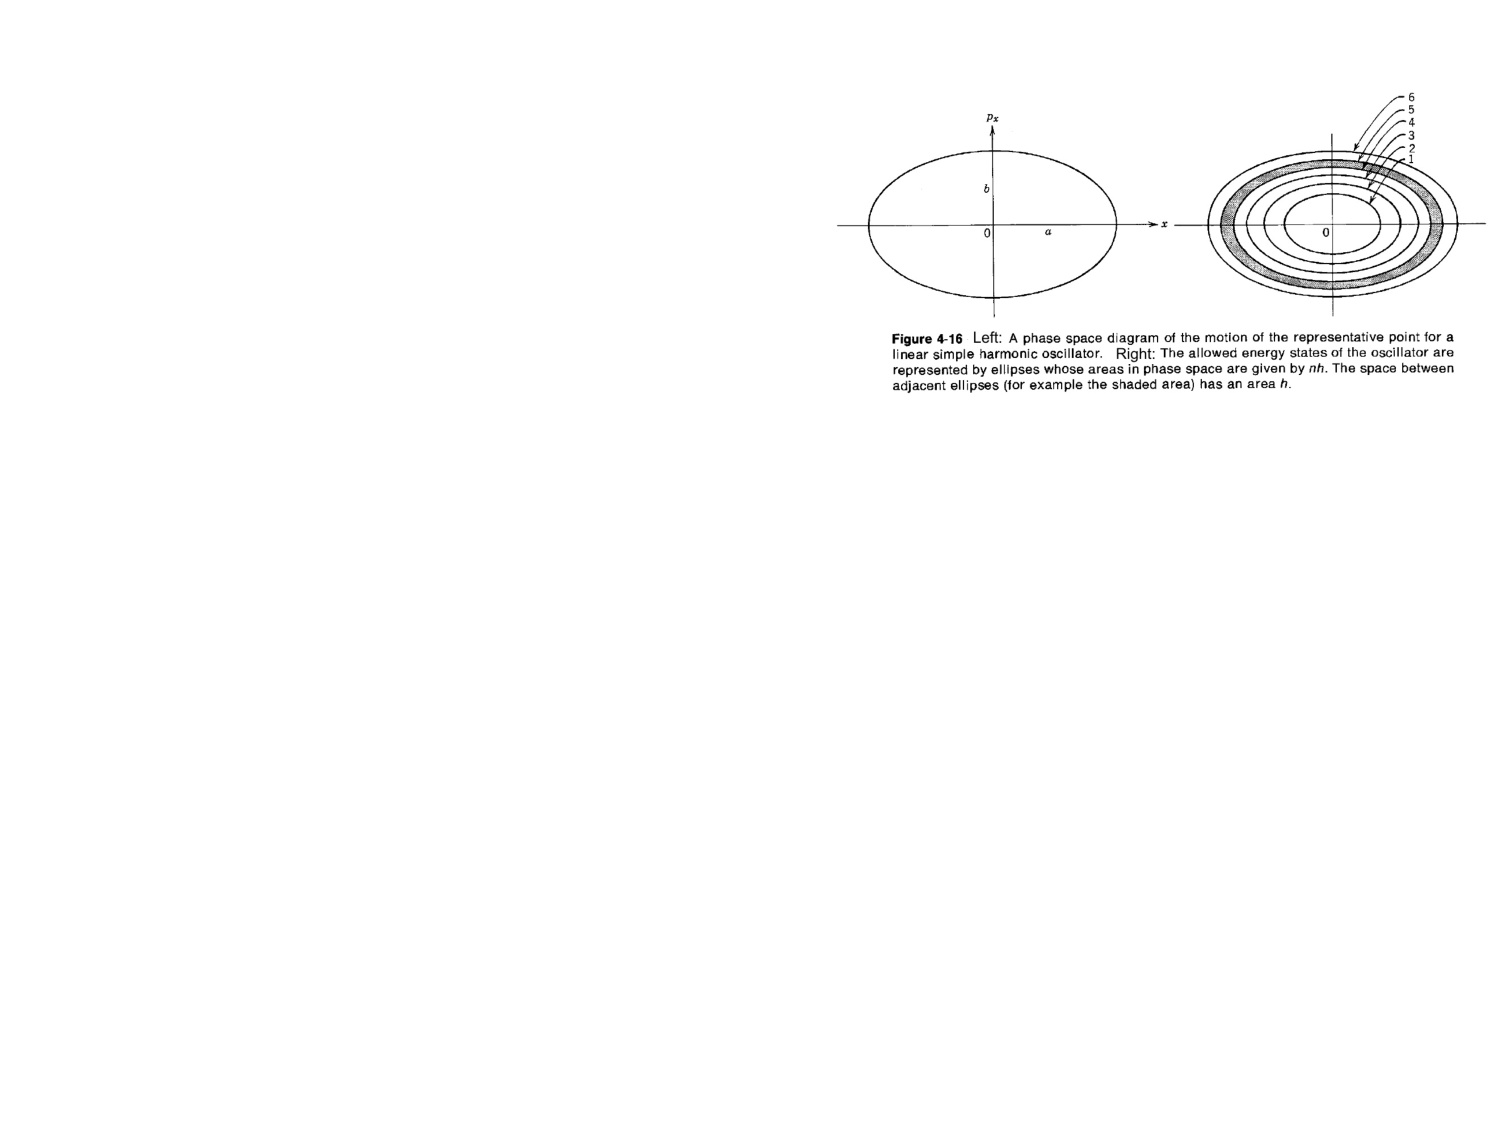
\includegraphics[scale=0.8]{/ellissi_spaziofasi}
\caption{Rappresentazione grafica dello spazio delle fasi di un oscillatore armonico}
\end{figure}

\paragraph{esempio: elettrone in orbita circolare}
Consideriamo un elettrone in un'orbita circolare con raggio $r$, in cui prendo come coordinata l'angolo $\theta$ funzione del tempo (andamento a "dente di sega"), allora il momento angolare è costante, $L = mvr = const$
\begin{equation}
\begin{split}
& \oint p_q dq = n_q h \oint L d\theta = n h \\
& \oint L d\theta = L \int_{0}^{2\pi} d\theta = 2\pi L
\end{split}
\end{equation}
da cui trovo ritrovo la \textbf{legge di quantizzazione del momento angolare} di Bohr
\begin{equation}
2\pi L = n h \quad\Rightarrow\quad L = \frac{ n h}{2 \pi } = n \hbar
\end{equation}

\paragraph{esempio: particella confinata}
Consideriamo una particella confinata in una dimensione, libera di muoversi, lungo l'asse $x$, da $-\frac{ a}{2 }$ a $+\frac{ a}{2 }$, che sono appunto gli estremi della "scatola" di lunghezza totale $a$.
Il momento $p$ della particella rimane costante cambiando segno ad ogni rimbalzo.
La regola di Wilson-Sommerfeld si traduce in
\begin{equation}
\begin{split}
& \oint p_x dx = p \oint dx = 2 p a = n h \\
& \frac{ n h }{p } = 2 a \quad\Rightarrow\quad n\lambda = 2a
\end{split}
\end{equation}
lo spazio $2a$ deve essere uguale ad un numero intero di lunghezze d'onda di De Broglie.
Significa che l'onda associata alla particella che si muove in una direzione è in fase con l'onda associata alla stessa particella che si muove nel verso opposto, la risultante è un'\textbf{onda stazionaria}.
La regola di quantizzazione di Wilson-Sommerfeld può essere intesa come la richiesta che l'onda di De Broglie associata alla particella confinata in moto periodico sia stazionaria.



    %%
%% Author: dariochinelli
%% 2021-03-23
%%

\section{Teoria quanto-meccanica di Shrodinger}
Con questa teoria è possibile esprimere l'equazione che controlla l'evoluzione di una funzione d'onda.
Essa è una funzione delle coordinate spaziali e del tempo, avente il significato di un'ampiezza di probabilità.
Sostanzialmente amplia il concetto dell'ipotesi di De Broglie.
Questa è l'espressione del moto di una particella libera con momento costante
\begin{equation}
\begin{split}
& \lambda = \frac{ h}{p } \\
& \Psi(x,t) = \sin \biggl[ 2 \pi \biggl( \frac{x}{\lambda} - \nu t \biggr) \biggr]
\end{split}
\end{equation}
Tuttavia se voglio considerare una particella con momento non costante, quindi su cui agisce una forza, essa è troppo semplice e occorre cercare un'equazione più complicata, che soddisfi le seguenti condizioni:
\begin{enumerate}
\item consistente con $\lambda = \frac{ h}{p }$ e $\nu = \frac{ E}{ h}$
\item consistente con $E = \frac{p^2}{2m} + V$
\item Lineare: ogni combinazione lineare di soluzioni deve essere anch'essa soluzione.
\item condizione di particella libera: $V(x,t) = V_0 = cost. \Rightarrow F=-\frac{ \partial V(x,t)}{ \partial x} = 0$
\end{enumerate}
Nel caso di particella libera la soluzione dovrà appartenere al campo complesso e avrà forma
\begin{equation}
\begin{split}
& \Psi (x,t) = \cos(kx-\omega t) + i \sin(kx - \omega t) \\
& \mbox{con} \quad k = \frac{2\pi}{\lambda}
\end{split}
\end{equation}


\paragraph{Equazione di Schrodinger} Nel 1925 Schrodinger postulò l'equazione per una particella quantistica:
\begin{equation}
- \frac{\hbar^2}{2m} \frac{\partial^2 \Psi(x,t)}{\partial x^2} + V(x,t) \Psi(x,t) = i \hbar \frac{\partial \Psi(x,t)}{\partial t}
\label{eq_schrodinger}
\end{equation}
Essendo $\Psi$ una funzione complessa cade l'idea di immaginarsi cosa ondeggi nel moto della particella.


\paragraph{Postulato di Born (1926)} Si può definire $P(x,t)$, che esprime la probabilità di localizzare una particella, come:
\begin{equation}
\begin{split}
P(x,t) dx & = \Psi^{\ast}(x,t)\Psi(x,t) dx \\
P(x,t) & = \Psi^{\ast}(x,t)\Psi(x,t) = |\Psi(x,t)|^2
\end{split}
\end{equation}


\subsection{Derivazione della TISE}
L'equazione di Shrodinger dipende dalle due variabili $x$ e $t$ ma si può risolvere mediante la \underline{tecnica di separazione delle variabili}, a patto che il potenziale non dipenda dal tempo ma solo da $x$
\begin{equation}
\begin{split}
& \Psi(x,t) = \psi(x)\varphi(t) \\
& -\frac{\hbar^2}{2m} \frac{\partial^2 \psi(x)}{\partial x^2}+ V(x)\psi(x) = E\psi(x)
\end{split}
\end{equation}
ottengo l'Equazione di Schrodinger indipendente dal tempo, si noti che non è esplicitamente un valore complesso.
E si trova, separatamente, la seguente soluzione per la parte temporale $\varphi$
\begin{equation}
\begin{split}
& \frac{d \varphi(t)}{dt} = - \frac{i E}{\hbar} \varphi(t) \\
& \varphi(t) = e^{-i \frac{E}{\hbar} t}
\label{eq_sch_temp}
\end{split}
\end{equation}

Come si arriva alla equazione di Schrodinger indipendente dal tempo
\begin{equation}
\begin{split}
& \frac{ p^2}{2m } + V = E \\
& p = \frac{ h}{\lambda } = \hbar k \quad \mbox{con } k = \frac{ 2\pi}{\lambda } \\
& \frac{ \hbar^2 k^2}{2m } + V = E \\
& k^2 \frac{ 2m}{\hbar^2 } (E-V)
\end{split}
\end{equation}
la funzione $\psi$ per una particella libera e le sue derivate sono
\begin{equation}
\begin{split}
\psi(x) & = \sin\frac{2\pi x}{\lambda } = \sin kx \\
\frac{ d \psi(x)}{dx } & = k \cos kx \\
\frac{ d^2 \psi(x)}{dx^2 } & = -k^2 \sin kx = -k^2 \psi(x) \\
\frac{ d^2 \psi(x)}{dx^2 } & = -\frac{ 2m}{\hbar^2 } (E-V) \psi(x) \\
-\frac{\hbar^2}{2m} \frac{\partial^2 \psi(x)}{\partial x^2} & + V(x)\psi(x) = E\psi(x)
\end{split}
\end{equation}
si ottiene così la funzione d'onda indipendente dal tempo, per ricavare il caso più generale si veda il corso di MQ.
Per postulato si afferma che questa equazione sia valida anche nel caso di una particella soggetta ad una forza.


\subsection{Particella libera} Soluzione per l'equazione di Schrodinger nel caso di una particella libera
\begin{equation}
\mbox{particella libera } \quad\Rightarrow\quad V(x) = costante \quad\Leftrightarrow\quad  F = - \frac{ dV(x)}{dx } = 0
\end{equation}
poiché il potenziale è una costante posso sceglierlo nullo, ovvero $V(x) = 0$.
L'equazione di Schrodinger indipendente dal tempo è
\begin{equation}
- \frac{ \hbar^2}{2m } \frac{ d^2 \psi(x)}{dx^2 } = E \psi(x)
\end{equation}
La soluzione generale dipendente dal tempo si ricava essere il prodotto tra la $\psi(x)$ soluzione all'equazione spaziale e la $\phi(t)$ soluzione all'equazione temporale \ref{eq_sch_temp} , ovvero
\begin{equation}
\Psi(x, t) = \psi(x) e^{ -\frac{ i E t}{\hbar } }
\label{psi_1}
\end{equation}
ed è anche vero che possiamo esprimere la funzione d'onda totale come 
\begin{equation}
\begin{split}
\Psi (x,t) & = \cos(kx-\omega t) + i \sin(kx - \omega t) \\
& = e^{ i (kx - \omega t) } = e^{ ikx } e^{ -i \omega t }
\end{split}
\label{psi_2}
\end{equation}
confrontando le due forme \ref{psi_1} e \ref{psi_2} di $\Psi(x, t)$ emerge subito l'equazione
\begin{equation}
\psi(x) = e^{ ikx }
\end{equation}
ricordando le forme di $k$ e $\omega$
\begin{equation}
k = \frac{ p}{\hbar } = \frac{ \sqrt{2mE}}{\hbar } \quad \quad \omega=\frac{ E}{\hbar }
\end{equation}
In effetti le soluzioni all'TISE (Time Indipendent Schrodinger Equation) sono due
\begin{equation}
\begin{split}
& \psi(x) = e^{ ikx } \\
& \psi(x) = e^{ - ikx }
\end{split}
\end{equation}
e quindi anche una combinazione lineare delle due deve essere una soluzione alla TISE
\begin{equation}
\psi(x) = A e^{ ikx } + B e^{- ikx }
\end{equation}
Se ho la condizione per cui $|A| = |B|$ si realizza il caso di onda stazionaria, ovvero ho due onde "viaggianti" in direzioni opposte.
Notare inoltre che in tale condizione la particella potrà trovarsi ovunque in $x$ e 
\begin{equation}
\begin{split}
\psi^{\ast}(x)\psi (x)= A^{\ast} A \quad\Rightarrow\quad  \Delta x = \infty \quad \Delta p = 0
\end{split}
\end{equation}
la notazione di Schrodinger deve necessariamente essere consistente con il Principio di Indeterminazione di Heisemberg.


\paragraph{Esempio: Buca infinita di potenziale}
Considero il caso 1-dimensionale, in cui la particella è confinata in una regione di spazio in cui il potenziale è nullo e fuori dal quale è infinito.
\begin{figure}[h]
\centering
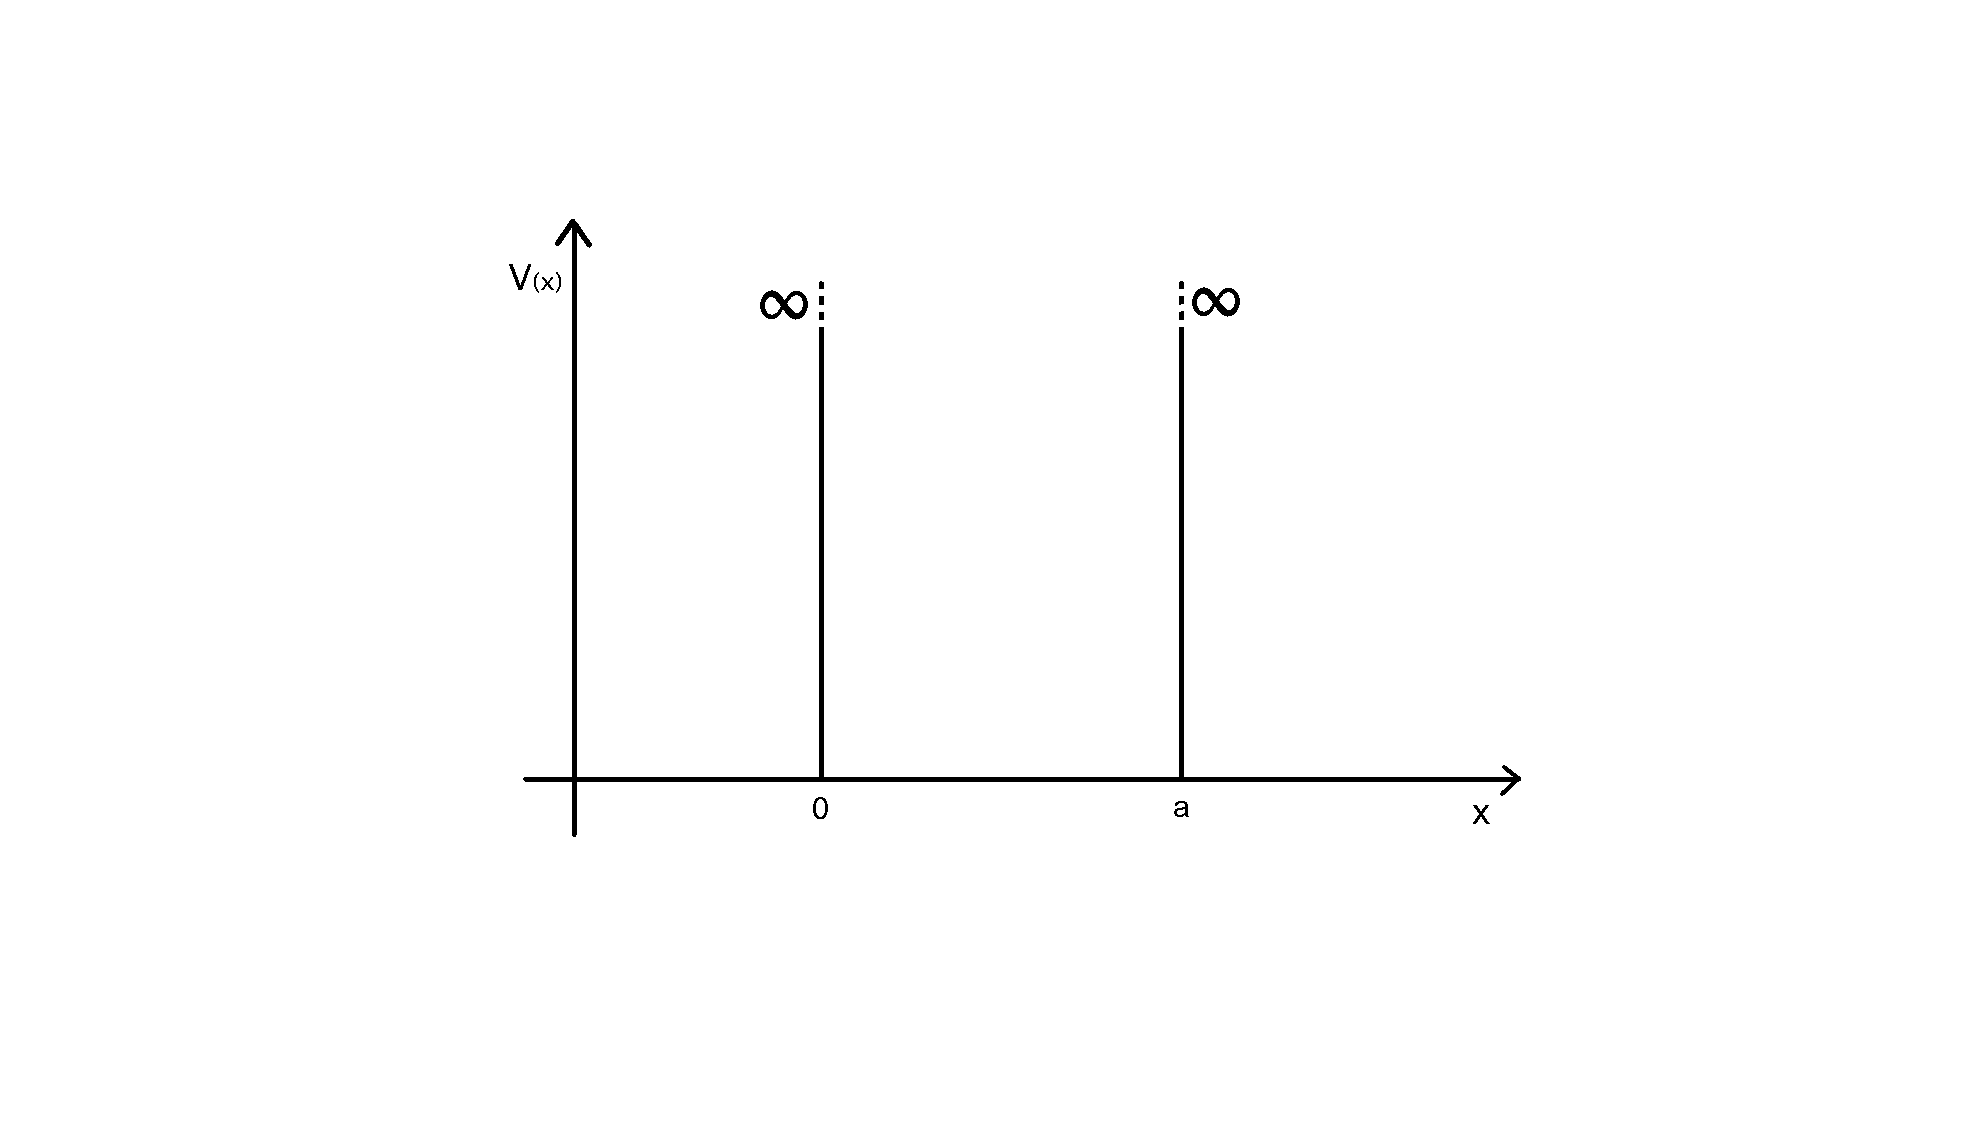
\includegraphics[scale=0.4]{/pot_inf}
\end{figure}
% potenziale buca infiinta
\begin{equation}
V(x) = 
\begin{cases}
	\infty \quad\quad x>a \vee x<0 & \quad\quad \mbox{regione \rm{I}} \\
	0 \quad\quad\quad 0 < x < a & \quad\quad \mbox{regione \rm{II}}
\end{cases}
\end{equation}
nella regione \rm{I} del potenziale la funzione d'onda dovrà essere nulla per cui $\psi(x)  = 0$, invece la funzione d'onda nella regione \rm{II} sarà $\psi (x) = A e^{i k x} + B e^{- i k x} $, quindi la particella è libera di muoversi avanti e indietro nell'intervallo $[0, a]$.
La funzione d'onda deve però essere stazionaria, non "viaggiante", poiché ha dei nodi fissi in corrispondenza degli estremi.
Quindi imponendo la condizione di annullamento di $\psi$ agli estremi ci permette di ricavare per l'estremo $x=0$
\begin{equation}
\begin{split}
& \psi(0) = A + B = 0 \quad\Rightarrow\quad  B = - A \\
& \Psi (x) = A ( e^{i k x} - e^{- i k x} ) = 2 i A \sin(k x) = c \sin(k x) \\
& \Rightarrow\quad c = 2 i A
\end{split}
\end{equation}
e per $x=a$
\begin{equation}
\begin{split}
& \psi(a) = c \sin(k a) = 0 \\
& \Rightarrow\quad c = 0 \quad \mbox{caso banale} \quad\Rightarrow\quad c\not= 0 \\
& \Rightarrow\quad \sin(k a) = 0 \quad\Leftrightarrow\quad ka = n \pi \quad \mbox{ con } n \in Z \\
& k = \frac{ n\pi}{a } \quad\Rightarrow\quad  p = \hbar k = \frac{ n \pi \hbar}{a }
\end{split}
\end{equation}
si ritrova la quantizzazione del momento $p$.
\begin{equation}
E = \frac{p^2}{2m} = \frac{\hbar^2 k^2}{2m} = \frac{\hbar^2 n^2 \pi^2 }{2 m a^2} \quad \mbox{ con } n \in Z
\end{equation}
A differenza della meccanica classica, in meccanica quantistica l'energia della particella (confinata) è quantizzata: può quindi assumere solo certi valori di energia \textit{permessi}.
\begin{equation}
\begin{split}
E & = \frac{ \hbar^2 \pi^2 n^2}{2ma^2 } \\
E_1 & = \frac{ \hbar^2 \pi^2}{2ma^2 } \\
E_2 & = 4 \frac{ \hbar^2 \pi^2}{2ma^2 } = 4 E_1 \\
E_3 & = 9 \frac{ \hbar^2 \pi^2}{2ma^2 } = 9 E_1
\end{split}
\end{equation}
Allora le funzioni d'onda per la particella corrispondenti ai diversi valori di $k$ sono
\begin{equation}
\psi_n(x) = c \sin\Bigl(  \frac{ n\pi x}{a }  \Bigr)
\end{equation}
sono le funzioni dell'ampiezza delle onde stazionarie all'interno della buca infinita di potenziale.
Il minimo dell'energia non è zero, bensì $E_1 = \frac{ \hbar^2 \pi^2}{2ma^2}$
è da notare che è una diretta conseguenza del principio di indeterminazione. 


\paragraph{Esempio: Particella in una scatola 3-D}
Il momento $p$ lungo le tre dimensioni sarà dipendente da tre numeri quantici $n_1,n_2,n_3$ e dalle tre dimensioni della scatola $a,b,c$, per cui
\begin{equation}
\begin{split}
p_x = \frac{\pi \hbar n_x}{a} \\
p_y = \frac{\pi \hbar n_y}{b} \\
p_z = \frac{\pi \hbar n_z}{c}
\end{split}
\end{equation}
Per cui l'energia risulta
\begin{equation}
E = \frac{p^2}{2m} = \frac{1}{2m} ( p_x^2 + p_y^2 + p_z^2 )= \frac{\pi^2 \hbar^2}{2m} \Bigl(  \frac{n_x^2}{a^2} + \frac{n_y^2}{b^2} + \frac{n_z^2}{c^2}  \Bigr)
\end{equation}
e l'equazione d'onda diventa
\begin{equation}
\psi(x) = c \sin \frac{n_1 \pi x}{a} \sin \frac{n_2 \pi x}{b} \sin \frac{n_3 \pi x}{c}
\end{equation}
Si ha una scatola cubica se $a=b=c$ per cui l'energia diventa
\begin{equation}
\begin{split}
E & = \frac{\pi^2 \hbar^2}{2 m a^2} r^2 \\ 
r^2 & = n_1^2 + n_2^2 + n_3^2
\end{split}
\end{equation}
Tutti gli stati energetici corrispondenti a diversi valori per $n_1^2, n_2^2, n_3^2$ che portano ad uno stesso valore di $r^2$ hanno la stessa energia, ma non hanno la stessa funzione d'onda.
Il fenomeno è detto di \textit{degenerazione}.
Per valori piccoli di $a$ i livelli energetici sono molto distanti fra loro, se aumento le dimensioni della scatola e $a$ è grande i livelli energetici saranno molto ravvicinati fino a formare quasi un continuo di stati.


\subsection{Densità di livelli energetici} 
Calcoliamo il numero di livelli energetici nel range $dE$ per una particella in una scatola cubica.
Nello spazio degli $n$, che è definito dalla terna $(n_x, n_y, n_z)$, ogni punto $P$ rappresenta un livello di energia possibile per la particella nella scatola cubica.
Tutti i punti che giacciono su una superficie di raggio $r$ hanno la stessa energia.
\begin{equation}
r^2 =  n_1^2 + n_2^2 + n_3^2
\end{equation}
% grafico ottante di sfera
\begin{figure}[h]
\centering
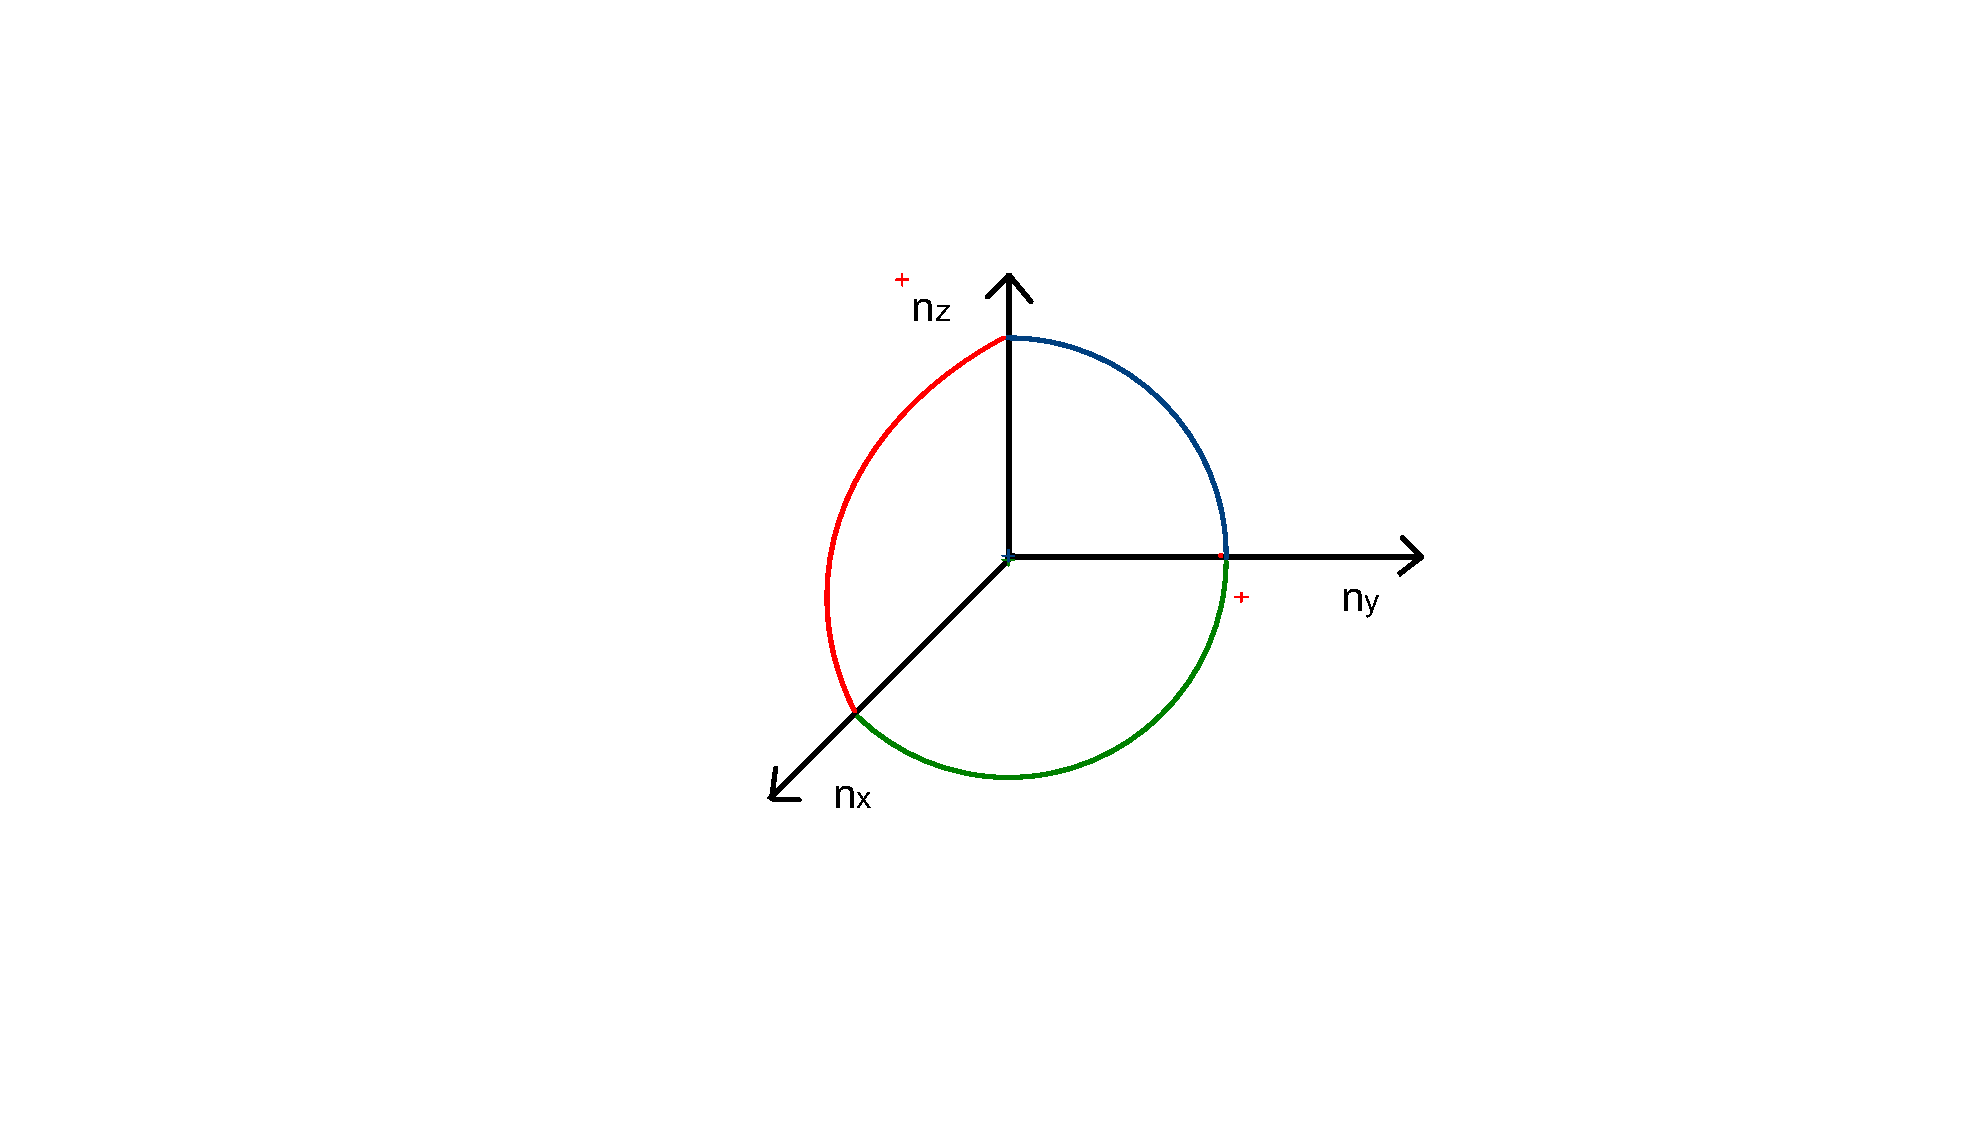
\includegraphics[scale=0.5]{/spazio_nodi}
\end{figure}
Per contare il numero di stati $N(E)$ che sono contenuti in un ottante di sfera calcoliamo il volume $(V=a^3)$ della sfera di raggio $r$ e moltiplichiamo per $\frac{1}{8}$
\begin{equation}
N(E) = \frac{1}{8} \Bigl( \frac{4}{3} \pi r^3 \Bigr) = \frac{\pi}{6} a^3 \Bigl( \frac{2 m E}{\pi^2 \hbar^2} \Bigr) ^{\frac{3}{2}} = 
\frac{8 \pi V}{3 h^3} (2 m^3) ^{\frac{1}{2}} E^{\frac{3}{2}}
\end{equation}
differenziando la relazione precedente si trova
\begin{equation}
dN(E) = \frac{4 \pi V (2 m^3)^{\frac{1}{2}} }{\hbar^3}  E^{\frac{1}{2}} dE
\end{equation}
Si introduce una \textit{funzione densità degli stati} $g(E)$ che definisce il numero di stati di energia possibile nell'intervallo $dE$, definita come
\begin{equation}
g(E) = \frac{ dN}{dE } = \frac{ 4\pi V (2m^3)^{\frac{ 1}{2 }}}{h^3 } E^{ \frac{ 1}{2 } }
\end{equation}
% grafico andamento g
\begin{figure}[h]
\centering
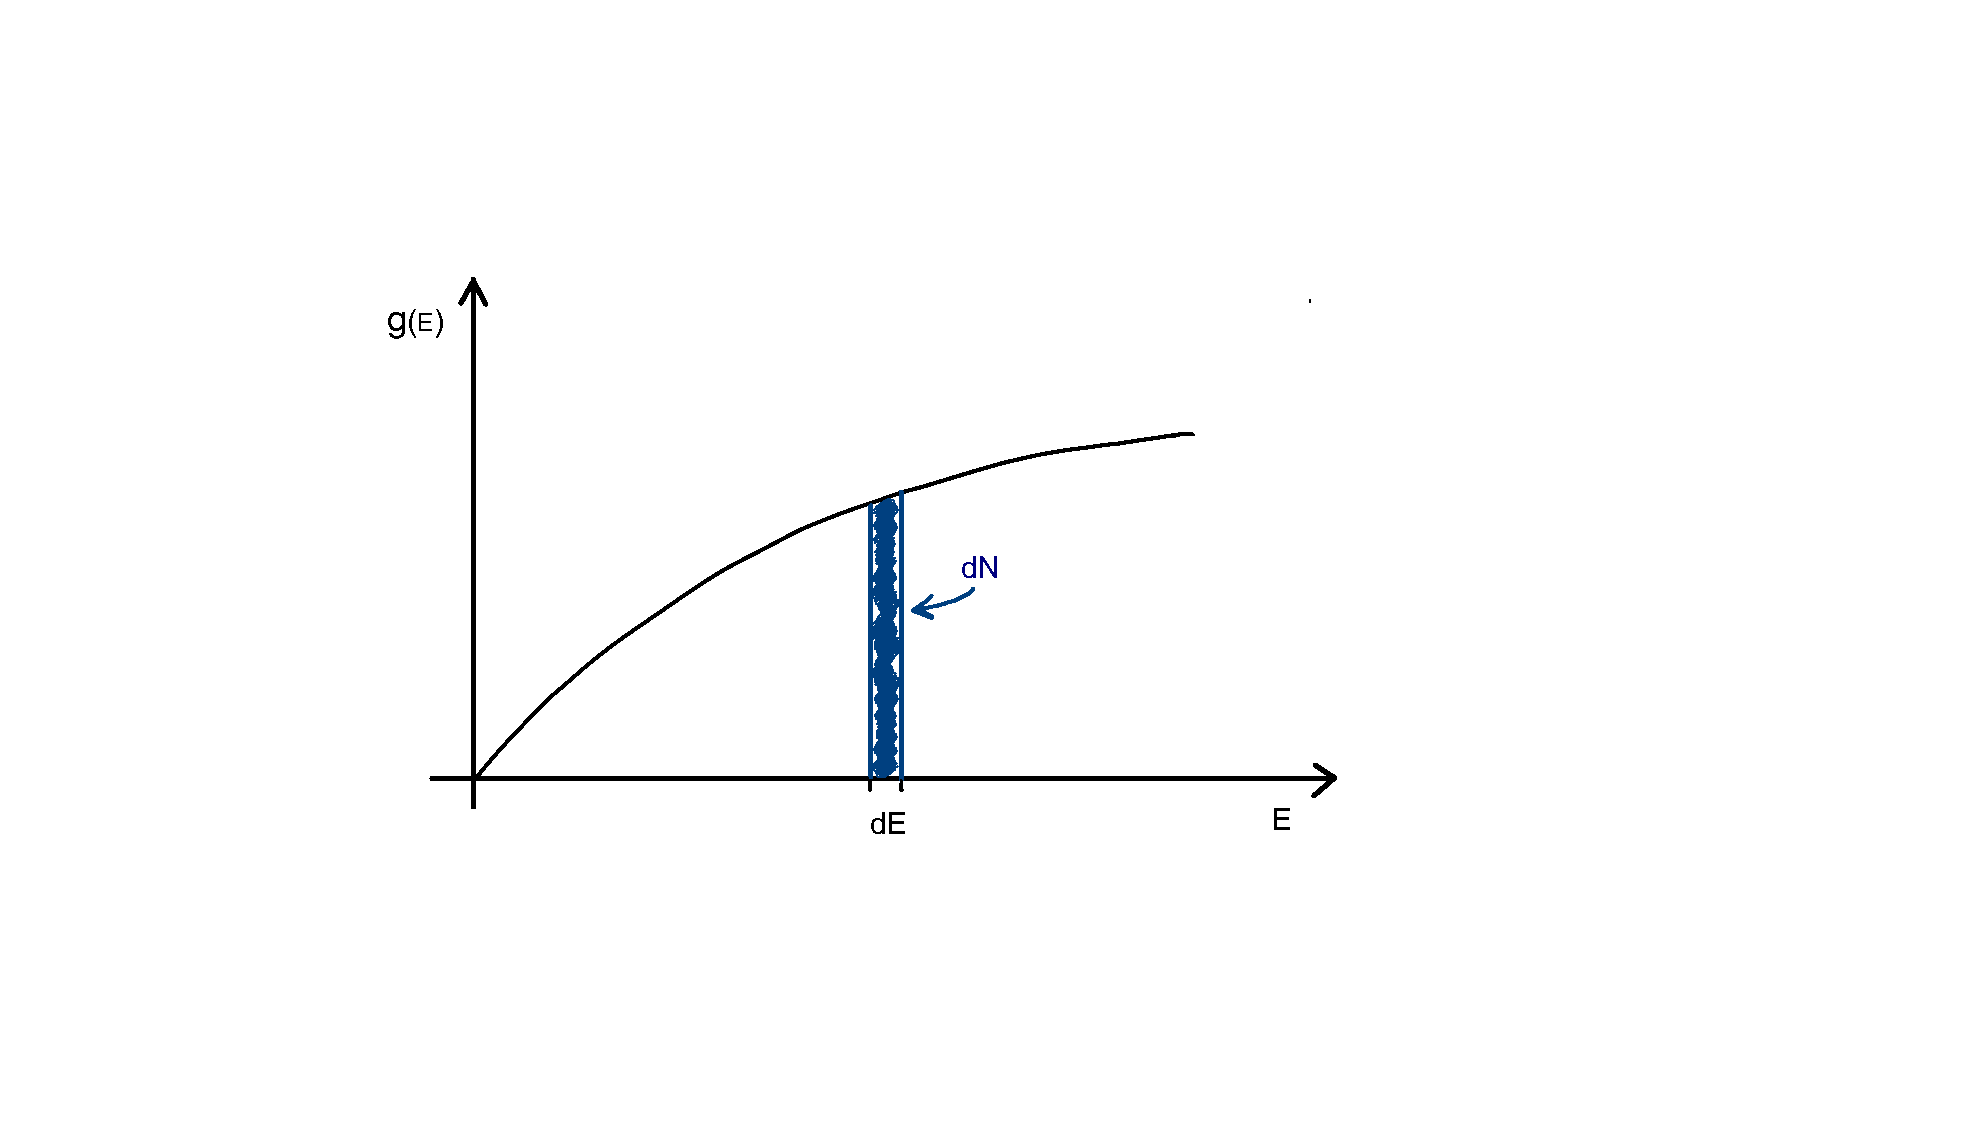
\includegraphics[scale=0.5]{/andamento_g}
\end{figure}
Posso allora definire una \textit{funzione densità degli stati} $g(p)$ dipendente dal momento $p$
\begin{equation}
\begin{split}
& dN = g(p)dp = g(E)dE \\
& \frac{ dN}{dp } = g(p) = g(E) \frac{ dE}{dp } = \frac{ 4\pi V}{h^3 } p^2
\end{split}
\end{equation}

\paragraph{Considero dei fotoni}
\begin{equation}
\begin{split}
& p = \frac{ h }{\lambda } \quad\quad \nu = \frac{ c}{\lambda } \\
& p = \frac{ h\nu}{c }
\end{split}
\end{equation}
Posso allora definire una \textit{funzione densità degli stati} $g(\nu)$ in funzione della frequenza $\nu$
\begin{equation}
\begin{split}
& g(\nu)d\nu = g(p)dp \\
& g(\nu) = g(p)\frac{ dp}{d\nu } = 2 \cdot \frac{ 4\pi V}{c^3 } \nu^2
\end{split}
\end{equation}
dove aggiungo un fattore $2$ poiché sto considerando dei fotoni, delle particelle con $spin=\frac{ 1}{2 }$, che hanno due possibili stati di polarizzazione.
Ottengo così alla relazione per il numero di modi delle frequenze permesse per le onde elettromagnetiche stazionarie nella cavità di corpo nero.
Il tipo di approccio di questi calcoli è simile a quanto visto contando le onde stazionarie come visto nel capitolo sul corpo nero.






    %%
%% Author: dariochinelli
%% 2020-10-13
%%

\section{Principio di Esclusione di Pauli}

Si consideri una scatola contenente due particelle. In Fisica Classica è sempre possibile distinguere il moto dell'una da quella dell'altra.
In Meccanica Quantistica invece, a causa del Principio di Indeterminazione, le due particelle sono indistinguibili poiché le due funzioni d'onda si sovrappongono.
Dunque occorre richiedere che tutti i risultati quanto-meccanici non devono perciò dipendere dall'assegnare un'etichetta a una particella piuttosto che ad un'altra.
È necessario scrivere quindi funzioni d'onda che tengano conto della instabilità delle particelle, le quali non interagiscono fra loro.
Partiamo scrivendo l'equazione di Schrodinger indipendente dal tempo per le due particelle:

\begin{equation}
- \frac{\hbar^2}{2m} \Bigl(  \frac{\partial^2 \Psi_T}{\partial x_1^2} + \frac{\partial^2 \Psi_T}{\partial y_1^2} + \frac{\partial^2 \Psi_T}{\partial z_1^2}  \Bigr) 
- \frac{\hbar^2}{2m} \Bigl(  \frac{\partial^2 \Psi_T}{\partial x_2^2} + \frac{\partial^2 \Psi_T}{\partial y_2^2} + \frac{\partial^2 \Psi_T}{\partial z_2^2}  \Bigr) 
+ V_T \Psi_T = E_T \Psi_T
\end{equation}

$$\mbox{In cui il potenziale usato è: } V_T = V(x_1, y_1, z_1) + V(x_2, y_2, z_2) $$

$$\mbox{In cui la funzione d'onda usata è: } \Psi_T = \Psi(x_1, y_1, z_1) \Psi(x_2, y_2, z_2) = \Psi_\alpha(1) \Psi_\beta(2)$$

Servono 3 numeri quantici per indicare le coordinate spaziali.
Poiché le particelle non sono distinguibili si potrebbe avere la particella 2 nello stato $\alpha$ e, viceversa, la particella 1 nello stato $\beta$.

Per la funzione d'onda è:

$$ \mbox{ 1) } \Psi_T = \Psi_\alpha(1) \Psi_\beta(2) $$
$$ \mbox{ 2) } \Psi_T = \Psi_\beta(1) \Psi_\alpha(2) $$

Cerchiamo la densità di probabilità della 1) e della 2):

$$ \mbox{ 3) } \Psi_\alpha^\ast(1) \Psi_\beta^\ast(2) \Psi_\alpha(1) \Psi_\beta(2) $$
$$ \mbox{ 4) } \Psi_\beta^\ast(1) \Psi_\alpha^\ast(2) \Psi_\beta(1) \Psi_\alpha(2) $$

Se scambio le "etichette" nella 3) cosa ottengo?

$$ \Psi_\alpha^\ast(2) \Psi_\beta^\ast(1) \Psi_\alpha(2)  \Psi_\beta(1) $$

che è un risultato diverso! Ciò significa che non tiene conto della indisitinguibilità.
Esistono due modi per scrivere funzioni d'onda che tengono conto di questo fatto:

$$ \mbox{a) } \Psi_s = \frac{1}{\sqrt{2}} \Bigl[ \Psi_\alpha(1) \Psi_\beta(2) + \Psi_\beta(1) \Psi_\alpha(2) \Bigr] \mbox{ soluzione simmetrica} $$
$$ \mbox{b) } \Psi_a = \frac{1}{\sqrt{2}} \Bigl[ \Psi_\alpha(1) \Psi_\beta(2) - \Psi_\beta(1) \Psi_\alpha(2) \Bigr] \mbox{ soluzione antisimmetrica} $$

Si tratta di due autofunzioni diverse per la stessa energia totale: si chiama \underline{degenerazione di scambio}
(dove per "scambio" si intende lo scambio delle "etichette").

Scambiamo quindi le etichette: 
$ 1 \to 2 $ e $ 2 \to 1 $

$$ \mbox{a) } \frac{1}{\sqrt{2}} \Bigl[ \Psi_\alpha(2) \Psi_\beta(1) + \Psi_\beta(2) \Psi_\alpha(1) \Bigr] = \Psi_s $$
$$ \mbox{b) } \frac{1}{\sqrt{2}} \Bigl[ \Psi_\alpha(2) \Psi_\beta(1) - \Psi_\beta(2) \Psi_\alpha(1) \Bigr] = - \Psi_a $$

Si dimostra che la densità di probabilità non cambia:

\begin{equation}
\begin{cases}
	\Psi_s^+ \Psi_s \to \Psi_s^\ast \Psi_s \\
	\Psi_a^+ \Psi_a \to (-1)^2 \Psi_a^\ast \Psi_a = \Psi_a^\ast \Psi_a
\end{cases}
\end{equation}

Nel 1925, Pauli preannuncia il suo celebre Principio di Esclusione: non ci può essere, nei sistemi multi elettronici, più di un elettrone in uno stesso stato quantico.

Cercando il contrario:
$$ \Psi_a = \frac{1}{\sqrt{2}} \Bigl[ \Psi_\alpha(1) \Psi_\alpha(2) - \Psi_\alpha(1) \Psi_\alpha(2) \Bigr] = 0 $$

Dunque la probabilità di trovare due elettroni nello stesso stato è nulla.
Se ne deduce che le particelle descritte da funzioni d'onda antisimmetriche, sono soggette al Principio di Esclusione di Pauli.
Tuttavia non tutte le particelle si comportano così, sperimentalmente si ricava la seguente tabella:

\begin{figure}[h]
\centering
\includegraphics[scale=0.7]{/particelle_simm_spin}
\caption{Tabella delle funzioni d'onda di alcune particelle note e spin}
\end{figure}

I \underline{bosoni} sono dunque particelle descritte da funzioni d'onda simmetriche ed i \underline{fermioni} da funzioni d'onda antisimmetriche.
Se si suppone che due particelle siano nello stesso stato quantico $(\alpha = \beta)$, allora si ha che:

$$ \Psi_T^\ast \Psi_T = \Psi_\beta^\ast(1) \Psi_\beta^\ast(2) \Psi_\beta(1) \Psi_\beta(2) $$

Nel caso di funzioni d'onda simmetriche si ottiene che la densità di probabilità è:

$$ \Psi_s^\ast \Psi_s = 2 \Psi_\beta^\ast(1) \Psi_\beta^\ast(2) \Psi_\beta(1) \Psi_\beta(2) = 2 \Psi_T^\ast \Psi_T \not = 0 $$

Se considero quindi due bosoni indistinguibili, la probabilità di trovarli in un certo stato è il doppio rispetto alla probabilità calcolata senza tenere conto della non distinguibilità.











\fi
    %%
%% Author: dariochinelli
%% 2021-03-25
%%

\section{Meccanica Statistica}
La meccanica statistica si utilizza in contesti in cui il sistema fisico è costituito da un elevato numero di elementi.
Se ad esempio consideriamo una mole di un gas stiamo considerando un sistema con \SI{6.02e23}{} particelle (corrispondente al numero di Avogadro $N_A$), risulterà quindi impossibile utilizzare un approccio in cui studiare il comportamento e l'evoluzione delle singole particelle.
Si usa allora un approccio statistico, mediando posizioni e velocità, questo metodo è utilizzato ad esempio per sistemi termodinamici.

\textit{Particella} viene utilizzato in senso ampio per indicare ogni unità ben definita che compone il sistema, potrà essere un atomo, una molecola, un elettrone e così via.

Considero un sistema di $N$ particelle
\begin{equation}
n_1,n_2,n_3, ...
\end{equation}
e considero che ogniuna abbia a disposizione diversi livelli di energia 
\begin{equation}
E_1,E_2,E_3, ...
\end{equation}
in cui si può trovare, tali stati potranno essere discreti e ben distanziati oppure tanto vicini da formare quasi un continuo.
Se assumiamo che tali stati siano discreti e che ogni particella $n_i$ si trovi in uno stato di energia $E_i$, allora il numero totale di particelle è dato da
\begin{equation}
N = n_1 + n_2 + n_3 + ... = \sum_s n_s
\end{equation}
che risulta essere una costante e l'energia totale del sistema è
\begin{equation}
U_{tot} = n_1 E_1 + n_2 E_2 + ... = \sum_s n_s E_s
\end{equation}
che, considerando un sistema isolato, risulta anch'essa una costante.

Esistono più distribuzioni possibili per le particelle fra i vari livelli energetici, che sono dette \textit{partizioni}, e per ogni stato macroscopico del sistema (definito da N, U, dal tipo di particella, ecc...) esiste una partizione più probabile delle altre.
Quando il sistema raggiunge la partizione più probabile allora il sistema è all'\textit{equilibrio statistico} e tenderà a rimanerci fintanto che non subentrerà un agente esterno.

Per studiare un sistema statistico dobbiamo trovare la partizione più probabile che corrisponde a trovare la legge di distribuzione, da cui potremo dedurre le proprietà macroscopiche del sistema che saranno le proprietà medie del sistema complessivo.

Come si ottengono le leggi di distribuzione? Vedremo ora tre casi:
la statistica classica, nel caso in cui le particelle siano distinguibili, e le statistiche quantistiche per indistinguibili, quindi bosoni e fermioni.


\subsection{Statistica classica di Maxwell Boltzmann}
La statistica di Maxwell-Boltzmann è anche detta statistica classica, assume che le particelle siano identiche e distinguibili, quindi possono essere etichettate eccetto per riarrangiamenti entro lo stesso stato di energia.
Vediamo ad esempio il grafico \ref{esempio_partizione} che rappresenta una possibile partizione tra i livelli energetici
\begin{figure}[h]
\centering
\includegraphics[scale=0.4]{/livelli_distr_particelle}
\caption{Esempio rappresentativo di una partizione, per la distribuzione di Maxwell-Boltzmann}
\label{esempio_partizione}
\end{figure}
Assumiamo che ognuno di questi livelli abbia la stessa probabilità di essere occupato.
La probabilità di una partizione è proporzionale al numero di modi differenti con cui le particelle possono essere distribuite tra i livelli di energia per produrre la partizione stessa.

Analizziamo ad esempio il caso in figura \ref{esempio_partizione}, vogliamo contare il numero di modi diversi con cui ottenere tale partizione.
Suppongo di avere un sistema a $N$ particelle.
Il modo di "piazzare" le prime tre particelle è dato dal prodotto
\begin{equation}
N (N-1) (N-2) = \frac{N!}{(N-3)!}
\end{equation}
\begin{figure}[h]
\centering
\includegraphics[scale=0.4]{/particelle_abc}
\caption{Esempio rappresentativo di una partizione, per la distribuzione di Maxwell-Boltzmann}
\label{esempio_partizione}
\end{figure}
Se le particelle fossero $a,b,c$, potrei sceglierle in 6 diversi ordini dati da
\begin{equation}
\begin{split}
& 3! = 6 \mbox{ diversi ordini} \\
& abc, bca, cab, bac, acb, cba
\end{split}
\end{equation}
questi 6 diversi ordini corrispondono alla stessa partizione, allora il numero precedente lo devo dividere per un fattore $3!$ ovvero
\begin{equation}
N (N-1) (N-2) = \frac{N!}{3!(N-3)!}
\end{equation}
Per cui generalizzando il problema: il numero di modi distinti $P_1$ di mettere $n_1$ particelle nel livello $E_1$ è
\begin{equation}
P_1 = \frac{ N!}{n_1! (N-n_1)! }
\label{stat_class}
\end{equation}
Considerando il secondo livello: ho a disposizione un numero $N-n_1$ particelle, per cui il numero di modi distinti $P_2$ di mettere $n_2$ particelle nel livello $E_2$ sarà dato da
\begin{equation}
P_2 = \frac{ (N-n_1)!}{n_2! (N-n_1-n_2)! }
\end{equation}
Analogamente per il terzo stato
\begin{equation}
P_3 = \frac{(N-n_1 - n_2)!}{n_3! ( N - n_1 - n_2 - n_3)!}
\end{equation}
Estendendo questo ragionamento a tutti i livelli si trova, moltiplicando tutte le $P_i$, il seguente risultato
\begin{equation}
W =  \frac{N!}{n_1! n_2! n_3! ... } = \prod_s P_s
\end{equation}
$W$ indica il numero di modi diversi totali per fare la partizione.
La probabilità di trovare la partizione è proporzionale al numero $W$, più tale numero è alto, più è alta la probabilità che quella partizione si realizzi.

\paragraph{Supponiamo livelli degeneri}
È necessario tener conto della correzione dovuta alla \textit{degenerazione}: più stati (diversi) corrispondono alla stessa energia, per cui ad esempio potrò distribuire le $n_1$ particelle che stanno nel livello $E_1$ in $g_1^{n_1}$ (inteso come $g_1$ elevato alla $n_1$) modi diversi.
Rispetto a quanto ricavato sopra, per il livello 1 il risultato si modifica con l'aggiunta del fattore motiplicativo $g_1^{n_1}$
\begin{figure}[h]
\centering
\includegraphics[scale=0.25]{/livelli_degeneri}
\caption{Livelli degeneri}
\label{esempio_partizione}
\end{figure}
\begin{equation}
P_1 = \frac{ N! g_1^{n_1}}{n_1! (N-n_1)! }
\end{equation}
analogo per tutti gli stati.
Il numero di modi totali distinti $W$ sarà quindi dato da
\begin{equation}
W(n_1,...,n_s) = \prod_{s=1}^{\infty} P_s = N! \prod_{s=1}^{\infty}\frac{ g_s^{n_s}}{ n_s!}
\end{equation}

\paragraph{La distribuzione più probabile è quella che massimizza il numero $W$} è il concetto chiave della meccanica statistica.
Vediamo ora come ricavare il set di numeri $n_1 ... n_s$ che massimizza $W$, tenendo presente le due condizioni iniziali: 
\begin{equation}
\begin{split}
N & =  \sum_{s=1}^{\infty} n_s \\
U & =  \sum_{s=1}^{\infty} n_s E_s
\end{split}
\end{equation}
il numero delle particelle iniziali $N$ è fisso e l'energia totale è costante $U$.

Se invece di massimizzare $W$ si massimizza $\ln(W)$, i prodotti diventano somme che mi agevolano i conti, questa operazione è consentita in quanto valida in generale tra $f(x)$ e $\ln(f(x))$.
Quindi significa risolvere la seguente equazione
\begin{equation}
\begin{split}
& \delta (\ln W) = 0 \\
& \delta (\ln W) = \sum_{s=1}^{\infty} \frac{ \partial (\ln W)}{\partial n_s } \delta n_s = 0
\end{split}
\label{massimizzare}
\end{equation}
$\delta n_s$ rappresenta la \textit{piccola variazione} sul numero $n_s$, che dovrà essere anch'essa compatibile con i due vincoli
\begin{equation}
\begin{split}
\delta N & = \sum_{s=1}^{\infty} \delta n_s = 0 \\
\delta U & = \sum_{s=1}^{\infty} E_s \delta n_s = 0
\label{vincoli}
\end{split}
\end{equation}
questo problema si risolve con il metodo dei \textit{moltiplicatori di Lagrange} accorpando le equazioni \ref{massimizzare} e \ref{vincoli}
\begin{equation}
\delta (\ln W)   - \alpha  \sum_{s=1}^{\infty} \delta n_s   - \beta  \sum_{s=1}^{\infty} E_s \delta n_s  = 0
\label{molti_lag}
\end{equation}
dove $\alpha$ e $\beta$ sono i coefficienti dei moltiplicatori di Lagrange, tali che $\alpha$ è il moltiplicatore collegato al vincolo riguardante il numero $N$ di particelle totali che è costante (prima equazione della \ref{vincoli}) e $\beta$ è il moltiplicatore collegato al vincolo riguardante l'energia $U$ del sistema costante (seconda equazione della \ref{vincoli}).
Riscriviamo allora l'equazione come 
\begin{equation}
\ln W = \ln N! + \sum_{s=1}^{\infty} (n_s \ln g_s - \ln n_s !)
\label{eq_max}
\end{equation}
e applichiamo l'\textit{approssimazione di Stirling} \ref{stirling}
\begin{equation}
\ln n! \to n \ln n - n \quad\quad \mbox{per } n \to \infty
\label{stirling}
\end{equation}
quindi l'equazione \ref{eq_max} diventa
\begin{equation}
\ln W = \ln N! + \sum_{s=1}^{\infty} (n_s \ln g_s - n_s \ln n_s + n_s)
\end{equation}

Ora usando l'equazione \ref{massimizzare} eseguiamo la derivata parziale in $n_s$ e otteniamo
\begin{equation}
\begin{split}
\delta (\ln W) & = \sum_{s=1}^{\infty} (\ln g_s - \ln n_s - 1 + 1) \delta n_s \\
\delta (\ln W) & = \sum_{s=1}^{\infty} (\ln g_s - \ln n_s ) \delta n_s
\end{split}
\end{equation}
l'equazione così ottenuta la sostituiamo nell'equazione \ref{molti_lag} in cui comparivano i moltiplicatori di Lagrange
\begin{equation}
\sum_{s=1}^{\infty} (\ln g_s - \ln n_s - \alpha - \beta E_s) \delta n_s = 0
\end{equation}
che sarà verificata per
\begin{equation}
\ln \frac{ n_s}{g_s } = -\alpha - \beta E_s
\end{equation}
quindi ottengo i valori di $n_s$ in funzione di $\alpha$ e $\beta$, da cui
\begin{equation}
\begin{split}
\frac{ n_s}{g_s } & = e^{ -\alpha - \beta E_s } \\
n_s & = g_s e^{ -\alpha - \beta E_s } \\
\frac{ n_s}{g_s } & = \frac{ 1}{ e^{ \alpha + \beta E_s }  }
\end{split}
\end{equation}
che corrispondono a tre modi equivalenti per indicare la \textit{Legge di distribuzione di Maxwell Boltzmann}.
Da cui possiamo ricavare la \textit{Funzione di Partizione} $Z$
\begin{equation}
\begin{split}
N & = \sum_{s=1}^{\infty} n_s = \sum_{s=1}^{\infty} g_s e^{ -\alpha } e^{ -\beta E_s } \\
e^{ -\alpha } & = \frac{ N}{ g_s  e^{ -\beta E_s }} = \frac{ N}{Z } \\
Z & =  \sum_{s=1}^{\infty} g_s e^{ -\beta E_s }
\end{split}
\end{equation}
e possiamo riscrivere la \textit{Legge di distribuzione di Maxwell Boltzmann} come
\begin{equation}
n_s = \frac{ N}{Z } g_s e^{ -\beta E_s }
\end{equation}
che è un'espressione dei numeri $n_s$ che massimizza il valore del numero $W$, ovvero la partizione più probabile.
Nella statistica classica di Maxwell Boltzmann $\frac{ n_s}{N }$ è la probabilità che una particella abbia energia $E_s$ e vale
\begin{equation}
\frac{ n_s }{N } = \frac{ 1}{Z } g_s e^{ -\beta E_s }
\end{equation}
che sarà anche la probabilità di occupazione del livello $E_s$.


\subsection{Statistica quantistica di Bose Einstein}
La Statistica quantistica di Bose Einstein si applica a particelle che non rispettano il Principio di esclusione di Pauli, quindi i bosoni.
Essendo particelle quantistiche e quindi non distinguibili non posso applicare la statistica classica \ref{stat_class}, ovvero non posso più contare le scelte possibili per una data particella ma considero il set di particelle tutto insieme e quello che devo considerare sono gli stati $g_s$ in un certo livello generico $E_s$ e contare il numero di modi in cui $n_s$ particelle possono andare nei $g_s$ stati del livello energetico $E_s$.
Supponiamo, ad esempio illustrativo, una schematizzazione di un unico generico livello $E_s$ come in figura \ref{livello_Es},
\begin{figure}[h]
\centering
\includegraphics[scale=0.3]{/livello_Es_1}
\caption{Livello energetico $E_s$, $n_s = 13$ particelle, $g_s = 10$ stati nel livello}
\label{livello_Es}
\end{figure}
otteniamo un diverso \textit{modo} cambiando il numero di particelle in uno o più stati, ma non otteniamo un \textit{modo} nuovo se scambiamo due particelle fra loro all'interno dello stesso stato o tra i diversi stati dello stesso livello.
Per contare il numero di modi utilizziamo il seguente ragionamento:
ci sono $g_s - 1$ linee di divisione tra gli stati
e ci sono $n_s + g_s - 1$ particelle + linee di divisione 
quindi nel caso in esempio ho: \\
$g_s - 1 = 10 - 1 = 9 $ \textit{linee di divisione} \\
$n_s + g_s - 1 = 13 + 10 - 1 = 22$ \textit{particelle + linee di divisione}. \\
Posso ottenere il seguente altro \textit{modo} di figura \ref{livello_Es_2} variando la composizione dei soli primi due stati 
\begin{figure}[h]
\centering
\includegraphics[scale=0.3]{/livello_Es_2}
\caption{Livello energetico $E_s$, $n_s = 13$ particelle, $g_s = 10$ stati nel livello}
\label{livello_Es_2}
\end{figure}
posso ottenerlo sia spostando una particella da uno stato all'altro sia spostando la linea di divisione e dividendo diversamente le particelle.
Quindi ci sono $(n_s + g_s - 1)!$ possibili permutazioni di particelle e linee di divisione che posso compiere, però alcune permutazioni non producono nuovi modi, quindi il numero totale di modi distinguibili di distribuire $n_s$ particelle nei $g_s$ stati del livello $E_s$ è
\begin{equation}
P_s = \frac{ (n_s + g_s - 1)!}{n_s! (g_s - 1)! }
\end{equation}
Per cui il numero di modi totali è
\begin{equation}
\begin{split}
W(n_1, ..., n_s) = \prod_{s=1}^{ \infty } P_s = \prod_{s=1}^{ \infty } \frac{ (n_s + g_s - 1)!}{n_s! (g_s - 1)! }
\end{split}
\end{equation}
Quindi ora, come visto nella statistica precedente, cerco di massimizzare il numero $W$, o meglio $\ln W$
\begin{equation}
\begin{split}
\ln W & = \sum_{s=1}^{\infty} \Bigl[ \ln ( n_s + g_s - 1 )! - \ln n_s ! - \ln (g_s - 1)! \Bigr] \\
\delta (\ln W) & = \sum_{s=1}^{\infty} \Bigl[ \ln(n_s + g_s) - \ln n_s \Bigr] \delta n_s
\end{split}
\end{equation}
utilizzando l'approssimazione di Stirling ed inserendo questo risultato nella \ref{molti_lag} ottengo l'equazione 
da cui posso ottenere i valori di $n_s$ in funzione di $\alpha$ e di $\beta$
\begin{equation}
\begin{split}
& \sum_{s=1}^{\infty} \Bigl[ \ln(n_s + g_s) - \ln n_s - \alpha -\beta E_s\Bigr] \delta n_s = 0 \\
& \ln \frac{ n_s}{n_s + g_s } = -\alpha - \beta E_s
\end{split}
\end{equation}
arrivando infine alla \textit{Legge di distribuzione di Bose Einstein}
\begin{equation}
\frac{ n_s}{g_s } = \frac{ 1}{e^{\alpha +\beta E_s} - 1 }
\end{equation}


\subsection{Statistica quantistica di Fermi Dirac}
La Statistica quantistica di Fermi Dirac si applica a particelle che obbediscono al Principio di esclusione di Pauli, quindi i fermioni.
Considero un livello energetico $E_s$ in cui ho $n_s$ particelle e $g_s$ stati disponibili e però devo tenere conto del principio di esclusione di Pauli, quindi devo contare i modi possibili per la partizione con la condizione che non ci sia più di una particella per ogni stato.
Possiamo allora dividere tutti gli stati in \underline{due gruppi}: $n_s$ sono tutti gli stati occupati e $(g_s - n_s)$ sono tutti gli stati non occupati.
Per cui il numero di modi è
\begin{equation}
P_s = \frac{ g_s !}{n_s! (g_s - n_s)! }
\end{equation}
che è analogo nella statistica classica per $P_1$ del primo livello...
Il numero totale $W$ è
\begin{equation}
W = \prod_{s=1}^{\infty} P_s = \prod_{s=1}^{\infty} \frac{ g_s !}{n_s! (g_s - n_s)! }
\end{equation}
quindi come nei casi precedenti: uso Stirling e differenzio
\begin{equation}
\begin{split}
\ln W & = \sum _{s=1}^{\infty} \Bigl[  \ln g_s! - \ln n_s! - \ln (g_s -n_s)!  \Bigr] \\
\delta (\ln W) & = \sum _{s=1}^{\infty} \Bigl[  - \ln n_s + \ln (g_s - n_s) - \alpha - \beta E_s  \Bigr] \delta n_s = 0 \\
& \ln \frac{ n_s}{g_s - n_s } = - \alpha - \beta E_s
\end{split}
\end{equation}
arrivando infine alla \textit{Legge di distribuzione di Fermi Dirac}
\begin{equation}
\frac{ n_s}{g_s } = \frac{ 1}{e^{ \alpha + \beta E_s } + 1 }
\end{equation}


\subsection{Plot delle statistiche}
Nei seguenti grafici sono riportati i plot di $\frac{ n_s}{g_s }$ in funzione di $E_s$, ponendo i parametri $\alpha=\beta=1$
\begin{figure}[h]
\centering
\includegraphics[scale=0.26]{/plot_stat_1}
\end{figure}
\begin{figure}[h]
\centering
\includegraphics[scale=0.37]{/plot_stat_2}
\end{figure}




    %%
%% Author: dariochinelli
%% 2021-03-27
%%

\section{Approfondimento sulla statistica classica di Maxwell-Boltzmann}

Riprendiamo la legge di distribuzione
\begin{equation}
n_s = \frac{N}{Z} g_s e^{ - \beta E_s }
\label{leg_dist_ns}
\end{equation}
legata alla funzione di partizione
\begin{equation}
Z = \sum_s e^{ - \beta E_s }
\label{fun_part}
\end{equation}
Dove i moltiplicatori di Lagrange $\alpha$ e $\beta$ sono legati al numero di particelle $N$ e all'energia $U$.
Il valore medio di una certa proprietà $F_{avg}$ dipendente dall'energia $E_s$
\begin{equation}
\begin{split}
F_{avg} = \langle F \rangle & =  \frac{1}{N} \sum_s n_s F(E_s) \\
& = \frac{1}{Z} \sum_s g_s F(E_s) e^{- \beta E_s}
\end{split}
\end{equation}

\subsection{Temperatura}
Classicamente la temperatura è stata introdotta per descrivere un'esperienza sensoriale, non statistica...
Facendo l'analisi dimensionale delle equazioni di $n_s$ e $Z$ si deriva che il fattore $\beta$ deve essere espresso in $1/joule$
affinché siano soddisfatte.

Se nell'espressione dell'energia sostituisco i valori $n_s$ della \ref{leg_dist_ns}, trovo
\begin{equation}
\begin{split}
U = n_1 E_1 + n_2 E_2 + ... & = \frac{ N}{Z } \Bigl(  g_1 E_1 e^{ -\beta E_1 } + g_2 E_2 e^{ -\beta E_2 } + ... \Bigr) \\
& = \frac{ N}{Z } \Bigl(  \sum_s g_s E_s e^{ -\beta E_s }  \Bigr)
\end{split}
\end{equation}
usando la definizione di funzione di partizione \ref{fun_part} si trova
\begin{equation}
\begin{split}
U &= - \frac{ N}{Z } \frac{ d}{d\beta }  \Bigl(  \sum_s g_s E_s e^{ -\beta E_s }  \Bigr) \\
& = - \frac{ N}{Z } \frac{ d Z}{d\beta } \\
& = - N \frac{ d}{d\beta }(\ln Z)
\label{energia_totale}
\end{split}
\end{equation}
L'energia media di ogni particella del sistema sarà
\begin{equation}
E_{avg} =  \langle E \rangle = \frac{ U}{N } = - \frac{ d}{d\beta } (\ln Z)
\label{energia_media}
\end{equation}
Da cui si vede che dato un certo sistema fisico descritto da valori $E_s$ e $g_s$ ben precisi, la funzione di partizione \ref{fun_part}, l'energia totale \ref{energia_totale} e l'energia media \ref{energia_media} risultano essere tutte funzioni di $\beta$;
significa che posso utilizzare $\beta$ per caratterizzare tutte queste funzioni.
Si trova però più conveniente introdurre un'altra variabile, funzione di $\beta$, ovvero la \textit{temperatura}, definita come:
\begin{equation}
\begin{split}
& k_B T = \frac{1}{\beta} \\
& k_B = \SI{1.3805e-23}{j / K} = \SI{8.6178e-5}{eV / K} \quad\quad \mbox{costante di Boltzmann}
\end{split}
\end{equation}
si noti che la grandezza $k_B T$ è un'\textit{energia termica}, ad esempio ponendoci a temperatura ambiente con $T_{amb}=\SI{300}{K}$ l'energia termica equivale a $k_B T_{amb} = \SI{0.0258}{eV} \simeq \SI{26}{m eV} $. \\
\textbf{NB:} Questa definizione di temperatura è valida solo per sistemi di particelle all'\textit{equilibrio statistico}. \\
Posso allora riscrivere le relazioni precedenti 
\begin{equation}
Z = \sum_s g_s e^{ - \frac{E_s}{k_B T} }
\end{equation}
\begin{equation}
n_s = \frac{N}{Z} g_s e^{ - \frac{E_s}{k_B T} }
\label{funz_dist_ns_T}
\end{equation}
il differenziale di $\beta$ è
\begin{equation}
d \beta = - \frac{d T}{k T^2}
\end{equation}
allora la relazione per l'energia totale è
\begin{equation}
U = k N T^2 \frac{d}{dT} (\ln Z)
\end{equation}
e l'energia media per particella è
\begin{equation}
\langle E \rangle = \frac{U}{N} = k T^2 \frac{d}{dT} (\ln Z)
\end{equation}
Il valore medio di una certa grandezza $F$ dipendente dall'energia è
\begin{equation}
\langle F \rangle = \frac{1}{Z} \sum_s g_s F(E_s) e^{ -\frac{E_s}{k_B T} }
\end{equation}
quindi la media di una funzione dipendente dall'energia è funzione della temperatura.
L'equazione \ref{funz_dist_ns_T} permette di capire che ad una certa temperatura $T$ fissata, l'occupazione di livelli di energia disponibili diminuisce all'aumentare della loro energia, si vanno ad occupare i livelli con energia sempre più elevata: 
quello che succede è che l'aumento di temperatura equivale all'aumento dell'energia totale delle particelle.
\begin{figure}[h]
\centering
\includegraphics[scale=0.35]{/livelli_occupati}
\caption{Grafico qualitativo della funzione di partizione \ref{funz_dist_ns_T} per diverse temperature }
\end{figure}

Il rapporto tra il numero di occupazione tra due stati generici $\frac{n_i}{n_j}$ è 
\begin{equation}
\begin{split}
\frac{n_i}{n_j} & = \frac{g_i}{g_j} e^{ - \frac{(E_i - E_j)}{k_B T} } \\
& = \frac{g_i}{g_j} e^{ - \frac{- \Delta E}{k_B T} }
\end{split}
\end{equation}
permette di capire che due livelli sono confrontabili se $\Delta E \ll k_B T$ e l'esponenziale tende a 1.


\subsection{Descrizione statistica del gas ideale}
La maggior parte dei gas possono essere descritti dalla statistica di Maxwell Boltzmann in un ampio range di temperature.
A seconda delle condizioni fisiche in cui ci troviamo, quindi a seconda della temperatura, della concentrazione del gas e quindi della massa totale delle particelle, un gas può comportarsi in modo classico o in modo quantistico, bosone o fermione. 
Allora a seconda della circostanza userò una delle tre statistiche viste sopra.

Applichiamo ora la statistica classica ad un gas ideale e monoatomico, costituito da particelle identiche e non interagenti, all'interno di un volume $V$:
in queste condizioni tutta l'energia delle particelle è energia cinetica.
Se il volume è grande il sistema ha un continuo di livelli energetici e posso riscrivere le leggi di MB passando al continuo

\begin{equation}
n(E)dE = \frac{N g(E) e^{-\beta E} dE}{\int_0^\infty g(E) e^{-\beta E} dE }
\label{numero_particelle}
\end{equation}

dove

\begin{equation}
Z = \int_0^{\infty} g(E) e^{ -\beta E } dE
\end{equation}

\begin{equation}
g(E) = \frac{4 \pi V (2m^3)^{ \frac{1}{2} }}{h^3} E^{ \frac{1}{2} }
\end{equation}





\newpage

I gas ideali, sistemi di particelle identiche non interagenti considerando poche moli in un gran volume.

Consideriamo un numero di particelle comprese nell'intervallo energetico $E$ e $E+dE$, cioè si considera la Funzione densità degli stati:
$$ n(E)dE = \frac{N g(E) e^{-\beta E} dE}{\int_0^\infty g(E) e^{-\beta E} dE } $$
si può definire a partire da questo approccio classico e non solo, come visto in precedenza nell'equazione di Schrodinger.

L'energia di una particella libera è:
\begin{equation}
E = K = \frac{p^2}{2m}
\mbox{ con }
\begin{cases}
p = (p_x, p_y, p_z) \\
q = (x, y, z)
\end{cases}
\end{equation}

Si postula quindi che il numero di stati di energia disponibili sia proporzionale, e finito, rispetto al volume nello spazio delle fasi.

\begin{gather*} 
 N(E) \propto \int d^3 p d^3 q = 4 \pi V \int p^2 dp \\
\mbox{pongo }  x = \frac{p}{\sqrt{2 m E}} \Rightarrow x^2 \leq 1 \\
N(E) \propto 4 \pi V \int_{x^2 \le 1}^{x > 0} x^2 (2mE)^{\frac{3}{2}} dx = 4 \pi V \Bigl[ \frac{x^3}{3}  \Bigr]_0^1 (2mE)^{\frac{3}{2}} = \frac{4}{3} \pi V (2m)^{\frac{3}{2}} E^{\frac{3}{2}}
\end{gather*}

$$  g(E)dE = \frac{dN(E)}{dE}dE \Rightarrow g(E)dE \propto 4 \pi V (2m^3)^{\frac{1}{2}} E^{\frac{1}{2}} dE $$

Nello spazio delle fasi ogni stato di energia non è rappresentato da un punto ma da un volume $V = h^3$, per Heisemberg $\Delta x \Delta p \simeq h$.
Dunque la correzione quantistica alla fisica classica consiste nello scrivere che:


\begin{equation}\label{ge_de}
g(E) dE = \frac{4 \pi V (2m^3)^{\frac{1}{2}} E^{\frac{1}{2}} dE}{h^3}
\end{equation}


Si considera ad esempio l'oscillatore armonico unidimensionale $ E = \frac{p^2}{2m} + \frac{K q^2}{2} $

\begin{gather*} 
N(E) \propto \int dp dq \\
\frac{p^2}{2mE} + \frac{K q^2}{2E} \leq 1 \mbox{ sostituendo: } 
\begin{cases}
	x = \frac{p}{\sqrt{2mE}} \\
	y = \frac{q}{\sqrt{2E}} \sqrt{K}
\end{cases} \\
N(E) \propto \int_{x^2 + y^2 = 1} dx dy \frac{2E}{\sqrt{K}} \sqrt{m}  \mbox{ con } \omega = 2 \pi \nu = \sqrt{\frac{K}{m}} \\
N(E) \propto \frac{E}{\nu} \Rightarrow g(E)dE \propto \frac{dE}{\nu}
\end{gather*} 

$$ \bar\varepsilon =  \frac{1}{N} \int_0^{\infty} n(\varepsilon) \varepsilon d\varepsilon = \frac{N}{N} \frac{\int_0^{\infty} g(\varepsilon) e^{- \beta E} \varepsilon dE}{\int_0^{\infty} g(\varepsilon) e^{- \beta \varepsilon} \varepsilon dE }$$

È la stessa formula usata per il corpo nero, in cui $P(\varepsilon) = C e^{- \frac{\varepsilon}{k T}} $ e $ C = \frac{1}{k T}$ valida se il numero di stati è indipendente dall'energia. Per il corpo nero $g(\varepsilon)$ è costante.

$$ \bar\varepsilon =   \frac{\int_0^{\infty} \varepsilon p(\varepsilon) d \varepsilon}{\int_0^{\infty} p(\varepsilon) d \varepsilon}$$

\begin{gather*} \label{fun_partizione}
g(E)dE = \frac{4 \pi V (2m^3)^\frac{1}{2}  E^\frac{1}{2} }{ h^3 } \\
Z =  \frac{4 \pi V (2m^3)^\frac{1}{2} }{ h^3 }  \int_0^{\infty}  E^\frac{1}{2} e^{- \frac{E}{k T}}  dE \\
\mbox{pongo: } \beta = \frac{1}{k T} \mbox{ \space ;  }  E = x^2  \rightarrow dE = 2x dx \\
Z =  \frac{4 \pi V (2m^3)^\frac{1}{2} }{ h^3 }  \int_0^{\infty}  E^\frac{1}{2} e^{- \frac{E}{k T}}  dE \\
= \frac{4 \pi V (2m^3)^\frac{1}{2} }{ h^3 } \int_0^{\infty} 2x^2 e^{- \beta x^2 } dx \\
= \frac{8 \pi V (2m^3)^\frac{1}{2} }{ h^3 } \Bigl[  \frac{1}{4} \sqrt{\frac{\pi}{\beta^3}}  \Bigr] 
= \frac{V (2 \pi m k T)^\frac{3}{2}}{h^3}
\end{gather*}

Abbiamo ottenuto la \underline{funzione di partizione per un gas monoatomico ideale}.
Applicando a destra e sinistra il logaritmo naturale ottengo:

$$ \ln (Z) = C + \frac{3}{2} \ln ( k T ) $$
$$ <E> = k T^2 \frac{d}{dT} (\ln Z)  \Rightarrow <E> = \frac{3}{2} k T$$
Che è l'energia cinetica media di Boltzmann, da cui si deduce che $\beta = (k T)^{-1}$.

$$  U_{tot} =  \frac{3}{2} k N T = \frac{3}{2} n k N_A T = \frac{3}{2} n R T $$

dove si vede $R = k N_A = \SI{8.3145}{J / mol * k}$

\begin{equation} 
n(E) dE = d n = \frac{N}{Z} e^{- \frac{E}{k T} } g(E) dE = \frac{N}{Z} \frac{4 \pi V (2m^3)^\frac{1}{2} E^\frac{1}{2} }{ h^3 } e^{- \frac{E}{k T}}  dE 
\end{equation}


\begin{equation} \label{formula_maxwell}
\frac{dn}{dE} = \frac{2 \pi N}{(\pi k T)^\frac{3}{2}} E^\frac{1}{2} e^{-\frac{E}{k T}}
\end{equation}

Abbiamo ottenuto così la \underline{formula di Maxwell}.

Infine dall'equazione dell'energia cinetica $E = \frac{1}{2} m v^2$

\begin{equation}
\frac{dn}{dv} = \frac{dn}{dE} \frac{dE}{dv} = mv \frac{dn}{dE} = 4 \pi N (\frac{m}{2 \pi k T})^\frac{3}{2} v^2 e^{- \frac{m v^2}{2 k T}}
\end{equation}

La formula $<E> = \frac{3}{2} k T $ è l'energia cinetica per particella e deriva dal \\
\underline{Teorema di Equipartizione dell'energia}, 
che afferma che ogni particella ha energia cinetica media pari a $\frac{1}{2} k T$ per ogni grado di libertà posseduto.




















    %%
%% Author: dariochinelli
%% 2021-03-31
%%

\section{Degenerazione statistica}
Riprendiamo le tre distribuzioni statistiche viste sopra
\begin{equation}
\begin{split}
\mbox{\underline{Maxwell-Boltzmann}}  \quad\quad  \frac{n_s}{g_s} & = \frac{1}{e^{\alpha + \beta E_s}} \\
\mbox{\underline{Bose-Einstein}}  \quad\quad  \frac{n_s}{g_s} & = \frac{1}{e^{\alpha + \beta E_s} - 1} \\
\mbox{\underline{Fermi-Dirac}}  \quad\quad  \frac{n_s}{g_s} & = \frac{1}{e^{\alpha + \beta E_s} + 1 } 
\end{split}
\end{equation}
Si nota subito che se 
\begin{equation}
e^{\alpha + \beta E_s} \gg 1
\label{condizione_e}
\end{equation}
allora si può trascurare l'$1$ a denominatore e applicare la statistica classica, questo implica
\begin{equation}
\frac{n_s}{g_s} \ll 1
\end{equation}
per cui la statistica di Maxwell Boltzmann si applica nel caso in cui il numero di particelle per stato sia molto minore di 1.
Se si prende come $zero$ il livello più basso dell'energia o \textit{livello fondamentale} $E_s = 0$, allora si ha che l'espressione \ref{condizione_e} è verificata per
\begin{equation}
e^{\alpha} \gg 1 \quad\Leftrightarrow\quad  e^{-\alpha} \ll 1
\end{equation}


\subsection{Parametro di degenerazione} Introduciamo il parametro di degenerazione $\xi$ tale che 
\begin{equation}
e^{-\alpha} = \xi 
\end{equation}
Se la condizione 
\begin{equation}
\xi = e^{-\alpha} \ll 1
\label{cond_deg}
\end{equation}
è verificata allora si dice che il gas è un \underline{gas non degenere} e posso utilizzare la statistica classica;
se al contrario la condizione \ref{cond_deg} non è soddisfatta allora il gas si definisce \underline{gas degenere} e dovrà essere descritto dalle statistiche quantistiche.

\paragraph{Esplicitiamo la condizione di degenerazione}
Riprendendo la relazione nel caso della statistica di MB
\begin{equation}
e^{\alpha} = \frac{Z}{N}
\end{equation}
e la funzione di partizione \ref{funzione_partizione_gasmono}
\begin{equation}
Z = \frac{V (2\pi m k_B T)^{ \frac{3}{2} }}{h^3}
\end{equation}
che si può riscrivere 
\begin{equation}
Z = \frac{V}{\lambda_{th}^3}
\end{equation}
in funzione del parametro $\lambda_{th}$ detto \textit{lambda termica di De Broglie}
\begin{equation}
\lambda_{th} = \Bigl(  \frac{h^2}{2 \pi m k_B T}  \Bigr)^{ \frac{1}{2} }
\label{lambda_th_debroglie}
\end{equation}
allora il parametro di degenerazione diventa
\begin{equation}
\begin{split}
& e^{\alpha} = \frac{V}{N} \frac{1}{\lambda_{th}^3} = \frac{1}{n} \frac{1}{\lambda_{th}^3} \\
\Rightarrow\quad & \xi = e^{-\alpha} = n \lambda_{th}^3
\label{disaccordo1}
\end{split}
\end{equation}
equivalente a
\begin{equation}
e^{-\alpha} = \frac{N}{Z} =  \frac{N h^3}{V (2 \pi m k T)^{\frac{3}{2}}} \ll 1
\end{equation}
La condizione \ref{cond_deg} si ottiene per
\begin{itemize}
\item piccole densità $\quad\Rightarrow\quad n$ piccolo 
\item alte temperature $\quad\Rightarrow\quad T$ grande $\quad\Rightarrow\quad \lambda_{th}$ piccolo
\end{itemize}


\subsection{Gas di bosoni} consideriamo un gas ideale di bosoni, quindi composto da particelle che seguono la statistica di Bose Einstein, situazione abbastanza comune poiché le molecole di un gas hanno in genere \textit{spin} intero $(0, 1, ...)$.
La legge di distribuzione di Bose Einstein, nel caso abbia un continuo di livelli di energia, la posso scrivere come
\begin{equation}
n(E)dE = g(E) \frac{1}{e^{ \alpha } e^{ \frac{E}{k_B T} } - 1 } dE
\end{equation}
in cui la \textit{funzione densità degli stati} è
\begin{equation}
g(E)dE = \frac{4\pi V (2m^3)^{ \frac{1}{2} }}{h^3} E^{\frac{1}{2} } dE
\end{equation}
allora il numero totale delle particelle nel sistema
\begin{equation}
N = \int_0^{\infty} n(E)dE =  \int_0^{\infty} \frac{g(E) dE}{e^{\alpha} e^{ \frac{E}{k_B T} } - 1} 
\end{equation}
risolviamo allora questo integrale, successivamente imponendo
\begin{equation}
x = \frac{E}{kT} \quad\quad Z = \frac{V (2 \pi m k_B T)^{ \frac{3}{2} } }{h^3}
\end{equation}
e trovo
\begin{equation}
\begin{split}
N & = \frac{4\pi V (2m^3)^{ \frac{1}{2} }}{h^3} \int_0^{\infty} \frac{E^{ \frac{1}{2} dE }}{e^{\alpha} e^{ \frac{E}{k_B T} } - 1}  \\
&= \frac{2Z}{\sqrt{\pi}} \int_0^{\infty} \frac{x^{ \frac{1}{2} }}{e^{ \alpha + x } - 1} dx
\label{integrale_num_part}
\end{split}
\end{equation}
\textbf{NB} per la statistica di BE il parametro $\alpha$ \underline{deve} essere positivo, per non avere il rapporto $\frac{n_s}{g_s}$ negativo.
Il denominatore nell'integrale precedente \ref{integrale_num_part} si può riscrivere come
\begin{equation}
(e^{ \alpha + x } - 1)^{-1} = e^{ - \alpha - x } (1 - e^{ - \alpha - x })^{ -1 }
\end{equation}
per cui l'integrale, in cui la parentesi risulta essere la serie geometrica che si può sviluppare in serie di Taylor
$$ \frac{1}{1-y} = 1 + y + y^2 + ... \quad\Rightarrow\quad \frac{1}{1 - e^{ -\alpha - x }} = 1 + e^{ - ( \alpha + x) } + e^{ - 2 ( \alpha + x) } + ... $$
l'integrale \ref{integrale_num_part} lo posso riscrivere e calcolare come segue 
\begin{equation}
\begin{split}
N & = \frac{2Z}{\sqrt{\pi}} \int_0^{\infty} \frac{x^{ \frac{1}{2} }}{e^{ \alpha + x }} \Bigl(  1 - e^{ - \alpha - x }  \Bigr)^{ -1 } dx \\ 
& = \frac{2Z}{\sqrt{\pi}} \int_0^{\infty} \frac{x^{ \frac{1}{2} }}{e^{ \alpha + x }} \Bigl(  1 + e^{ - (\alpha + x) } + e^{ - 2 (\alpha + x) } + ...   \Bigr)
dx \\ &= Z e^{ -\alpha } \Bigl(  1 + \frac{1}{2^{\frac{3}{2}}}e^{ -\alpha } + \frac{1}{3^{\frac{3}{2}}} e^{ -2\alpha } + ...  \Bigr)
\end{split}
\end{equation}
da cui allora ricavo
\begin{equation}
e^{ -\alpha } = \frac{N}{Z} \Bigl(  1 + \frac{1}{2^{\frac{3}{2}}}e^{ -\alpha } + \frac{1}{3^{\frac{3}{2}}} e^{ -2\alpha } + ...  \Bigr)^{ -1 }
\end{equation}
fermandomi al primo termine $\quad\Rightarrow\quad $ \textbf{risultato classico}
\begin{equation}
e^{ -\alpha } = \frac{N}{Z} \quad\Rightarrow\quad e^{ \alpha } = \frac{Z}{N}
\end{equation}
fermarsi al primo termine significa assumere che $e^{ -\alpha } \ll 1$, appunto. \\
Calcoliamo ora l'\textbf{energia totale del sistema}, calcolando un integrale analogo al precedente tranne che per la dipendenza dalla temperatura $T$ a numeratore e la variabile integranda $x^{ \frac{3}{2} }$ 
\begin{equation}
\begin{split}
U & = \int_0^{\infty} E n(E)dE = \frac{2Zk_B T}{\sqrt{\pi}} \int_0^{\infty} \frac{x^{ \frac{3}{2} }}{e^{ \alpha + x } - 1 } dx \\
& = \frac{3}{2} k_B T Z e^{ -\alpha } \Bigl(  1 + \frac{1}{2^{ \frac{2}{5} }} e^{ -\alpha } +  \frac{1}{3^{ \frac{2}{5} }} e^{ -2 \alpha } + ... \Bigr)
\end{split}
\end{equation}
fermandomi al primo ordine
\begin{equation}
\begin{split}
U & = \frac{3}{2} k_B T Z e^{ -\alpha } \\
& = \frac{3}{2} k_B T Z \frac{N}{Z} = \frac{3}{2} N k_B T
\end{split}
\end{equation}
ricordando che $e^{ -\alpha } = \frac{N}{Z}$, ritrovo allora l'energia totale di un gas classico. \\
Da cui ricavo inoltre l'energia media per particella nel risultato classico
\begin{equation}
\frac{U}{N} = \langle E \rangle = \frac{3}{2} k_B T
\end{equation}
Fermandomi invece al secondo ordine
\begin{equation}
\bar U = \frac{U}{N} = \frac{3}{2} k_B T \Bigl[  1 - \frac{1}{2^{ \frac{5}{2} }}  \frac{N h^3}{V (2\pi m k_B T)^{ \frac{3}{2} }}  \Bigr]
\end{equation}
il secondo termine in parentesi esprime la \textit{deviazione} di un \textbf{gas di bosoni} rispetto ad un gas classico, per cui
\begin{equation}
\xi = \frac{N h^3}{V (2\pi m k_B T)^{ \frac{3}{2} }}  \ll 1 
\end{equation}
è la condizione per la statistica classica, che è proprio la quantità $e^{-\alpha}$ ovvero $\xi$.
Ciò significa che nel caso quantistico di \textit{bosoni}, rispetto ad un caso classico, l'energia del sistema sarà un po' \textbf{inferiore}:
la probabilità di trovare due particelle in uno stesso stato di energia è più grande per un gas di bosoni che per un gas classico, \textit{"i bosoni preferiscono stare in uno stesso stato"}.
Da questo ragionamento discende inoltre che un gas di bosoni ha una \textit{pressione inferiore} rispetto al gas classico, dovuto al fatto che hanno una energia media per particella inferiore.


\subsection{Gas di fermioni} Rifacendo tutto lo stesso ragionamento utilizzando la statistica di Fermi Dirac, quindi per un \textbf{gas di fermioni}, trovo che l'energia media per ogni fermione è 
\begin{equation}
\bar U = \frac{U}{N} = \frac{3}{2} k_B T \Bigl[  1 + \frac{1}{2^{ \frac{5}{2} }} \frac{N h^3}{V (2\pi m k_B T)^{ \frac{3}{2} }} \Bigr]
\end{equation}
il secondo termine in parentesi esprime la \textit{deviazione} di un \textbf{gas di fermioni} rispetto ad un gas classico, per cui
\begin{equation}
\xi = \frac{N h^3}{V (2\pi m k_B T)^{ \frac{3}{2} }}  \ll 1 
\end{equation}
è la condizione per la statistica classica, che, anche qui, è proprio la quantità $e^{-\alpha}$ ovvero $\xi$.
Ciò significa che nel caso quantistico di \textit{fermioni}, rispetto ad un caso classico, l'energia del sistema sarà un po' \textbf{maggiore}:
la probabilità di trovare due particelle in uno stesso stato di energia è nulla per un gas di fermioni che per un gas classico, infatti obbediscono al Principio di Esclusione di Pauli, \textit{"i fermioni preferiscono stare da soli in uno stesso stato"}.
Da questo ragionamento discende inoltre che un gas di bosoni ha una \textit{pressione maggiore} rispetto al gas classico, dovuto al fatto che hanno una energia media per particella maggiore.

\paragraph{NB:}
\textit{Ogni volta che la distanza tra le particelle diventa confrontabile o più piccola della lunghezza d'onda di De Broglie a loro assegnata, ci aspettiamo di osservare effetti quantistici, caso in cui le funzioni d'onda delle particelle si sovrappongono e non posso più trattarle classicamente.} \\
Supponiamo di avere un gas all'equilibrio ad una certa temperatura $T$, l'energia cinetica media per particella ed il momento medio sono
\begin{equation}
K_{media} = \frac{3}{2} k_B T
\quad\quad\quad
p_{medio} = \sqrt{2mK} = \sqrt{3 m k_B T}
\end{equation}
La lambda di De Broglie è \textit{proporzionale} alla \ref{lambda_th_debroglie} lambda termica di De Broglie $\lambda_{th}$, per cui
\begin{equation}
\lambda = \frac{h}{p} 
= \frac{h}{(3mk_B T)^{ \frac{1}{2} }}
= \Bigl(  \frac{2\pi}{3}  \Bigr)^{ \frac{1}{2} }\Bigl(  \frac{h^2}{2\pi mk_B T}  \Bigr)^{ \frac{1}{2} }
= \lambda_{th} \sqrt{\frac{2\pi}{3}} 
\end{equation}
Supponiamo allora di avere un sistema di $N$ particelle in un volume $V$, per cui il \textit{volume medio} per ogni particella e quindi la \textit{distanza media} saranno rispettivamente
\begin{equation}
d^3 = \frac{V}{N}
\quad\quad\quad
d = \Bigl(   \frac{V}{N}  \Bigr)^{\frac{1}{3}}
\end{equation}
gli \textit{effetti quantistici} sono importanti se
\begin{equation}
\lambda \ge d
\end{equation}
da cui sostituendo si trova quanto segue, da $(\ast)$ si trovano due risultati in parallelo:
\begin{equation}
\begin{split}
\Bigl(  \frac{2\pi}{3}  \Bigr)^{ \frac{1}{2} } \Bigl(  \frac{h^2}{2\pi mk_B T}  \Bigr)^{ \frac{1}{2} }  & \ge \Bigl(   \frac{V}{N}  \Bigr)^{\frac{1}{3}} \\
\frac{N}{V} \Bigl(  \frac{h^2}{2\pi mk_B T}  \Bigr)^{ \frac{3}{2} } & \ge \Bigl(  \frac{3}{2\pi}  \Bigr)^{ \frac{3}{2} }  \\
(\ast) & \\
\xi \ge  \Bigl(  \frac{3}{2\pi}  \Bigr)^{ \frac{3}{2} } \approx 0.33
\quad\quad\quad & \quad\quad
\frac{N}{V} \lambda_{th}^3 = n\lambda_{th}^3 \ge  \Bigl(  \frac{3}{2\pi}  \Bigr)^{ \frac{3}{2} } \approx 0.33
\end{split}
\end{equation}
in cui $\xi$ è il parametro di degenerazione
\begin{equation}
\xi = \frac{N h^3}{V(2\pi mk_B T)^{ \frac{3}{2} }}
\end{equation}
per cui si ottiene
\begin{equation}
\xi = \frac{N}{V} \lambda_{th}^3 = n \lambda_{th}^3
\end{equation}
Risultato in accordo con la \ref{disaccordo1}.

\textbf{Concludo} che il parametro di degenerazione deve essere maggiore di $\approx \frac{1}{3}$ affinché siano consistenti gli effetti quantistici, per cui il gas è degenere.
Intorno alla temperatura ambiente, per normali gas, si ha $\xi \ll 1$ e posso trattare il sistema con la statistica di Maxwell Boltzmann.
Se la temperatura è sufficientemente alta che la lambda termica di De Broglie $\lambda_{th}$ è molto più piccola della distanza fra particelle, allora un gas si comporta classicamente e posso applicare la statistica di Maxwell Boltzmann. 
Quando la massa $m$ diventa piccola o la temperatura $T$ diventa molto bassa o quando la densità $\frac{N}{V}$ diventa elevata dovrò considerare effetti quantistici.







    %%
%% Author: dariochinelli
%% 2021-1-23
%%

\section{Gas di elettroni}

Gli elettroni sono fermioni, la loro statistica è perciò descritta dal modello di Fermi-Dirac, poiché si tratta di particelle soggette al principio di esclusione di Pauli.

Sostituisco nella formula di Fermi-Dirac

\begin{equation}
\frac{n_s}{g_s} = \frac{1}{e^{\alpha + \beta E_s} + 1 } \quad \mbox{con} \quad
	\begin{cases}
		\alpha = - \frac{ E_F}{k T } \quad \mbox{con $E_F$ funzione della temperatura} \\
		\beta = \frac{ 1}{k T }
	\end{cases} \\
\end{equation}

\begin{equation}
\frac{n_s}{g_s} = \frac{1}{e^{\alpha + \beta E_s} + 1 }
= \frac{ 1}{e^{ \frac{ E_s - E_F}{k T } } +1 }
\end{equation}

Quando $E_s = E_F$ si ha che $\frac{ n_s}{g_s } = \frac{ 1}{2 }$ \\
e ciò è particolarmente evidente per $T \not = 0$, infatti $\lim_{T \to 0} \frac{ n_s}{g_s } = 0$

Si definisce $E_F(T)$ l'\underline{energia di Fermi}, e si parla di \underline{livello di Fermi} quando si ha $E_F(0)$. Valutiamo ora lo studio di funzione di $\frac{ n_s}{g_s }$ al variare di $T$. \\

Analizziamo tre casi significativi dell'andamento del rapporto $\frac{ n_s}{g_s }$ rispetto a diverse temperature:

\begin{figure}[h]
\centering
\includegraphics[scale=0.13]{/Gas_elettroni_temperature}
\caption{Grafici casi limite temperature gas di elettroni}
\end{figure}

\begin{enumerate}[label=(\alph*)]
\item Caso $T = 0$ quindi $\alpha = - \infty$,  gli stati di più bassa energia vengono occupati per primi, gli altri a seguire. 
In accordo con il Principio di esclusione di Pauli.
\item Caso $T \not = 0$  con $T \ll T_F$ \quad $\Bigl( dove T_F = \frac{ E_F(0)}{K }   \Bigr)$, si può notare come la funzione a gradino si modifichi lievemente,
il disegno non è in scala ma rende l'idea, è noto che $E_F(0) \gg kT$.
Siamo infatti in una situazione per cui la differenza dal caso precedente è minima, poiché in tale condizione $E_F(T) \sim E_F(0)$.
L'energia termica del sistema è usata per promuovere i fermioni dagli stati di energia un po' sotto $E_F$ agli stati un po' sopra $E_F$, 
in particolare la variazione di energia è ristretta ad una regione (del grafico) di lunghezza $kT$, che è l'energia di ogni particella.
\item Ad alte temperature abbiamo $T \gg T_F$ il numero di particelle per stato quantistico per la distribuzione classica è più piccolo di 1,
le distribuzioni quantistiche si fondono con quella classica.
\end{enumerate}

Calcoliamo ora il numero di particelle: dalla statistica di Fermi-Dirac si ha che

\begin{gather*} 
n(E)dE = \frac{ g(E)}{e^{ \frac{ E - E_F}{kT } } + 1 } \\
\mbox{dove} \quad g(E)= \frac{4 \pi V (2m^3)^{\frac{1}{2}} E^{\frac{1}{2}}}{h^3} \\
\mbox{spin } \Bigl(  \pm \frac{ 1}{2 }  \Bigr) \Rightarrow \quad g(E)= \frac{8 \pi V (2m^3)^{\frac{1}{2}} E^{\frac{1}{2}}}{h^3}
\end{gather*}

trattandosi di elettroni occorre moltiplicare per due a causa della doppia possibilità dello spin

\begin{equation}
N = \int_0^{\infty} n(E)dE = \int_0^{\infty} \frac{8 \pi V (2m^3)^{\frac{1}{2}} E^{\frac{1}{2}}}{h^3} \frac{ dE}{e^{ \frac{ E-E_F}{kT } } + 1 }
\end{equation}

Notiamo che allo zero assoluto si ha che 

\begin{equation}
\frac{ 1 }{e^{ \frac{ E - E_F}{kT } } + 1 } = 1 \quad
\mbox{come una funzione a gradino: } \quad
\begin{cases}
	1 \quad 0 \le E \le E_F \\
	0 \quad > E_F
\end{cases}
\end{equation}
dunque si semplifica scrivendo che 

\begin{equation}
\begin{split}
N = \int_0^{E_F(0)} g(E)dE & =  \int_0^{E_F(0)} \frac{8 \pi V (2m^3)^{\frac{1}{2}} E^{\frac{1}{2}}}{h^3} dE \\
& = \frac{16 \pi V (2m^3)^{\frac{1}{2}} }{3 h^3} [E_F(0)]^{\frac{3}{2}}
\end{split}
\end{equation}

\begin{equation}
\Longrightarrow \quad E_F(0) = \frac{ h^2}{8m } \Bigl(  \frac{ 3}{\pi } \frac{ N}{V }  \Bigr)^{ \frac{ 3}{ 2} } = \frac{ h^2}{8m } \Bigl(  \frac{ 3}{\pi } n \Bigr)^{ \frac{ 3}{ 2} }
\end{equation}

dove $n = \frac{ N}{V }$.
Da un punto di vista matematico si è calcolato l'area del sottografico come in figura

\begin{figure}[h]
\centering
\includegraphics[scale=0.07]{/gas_elettroni_areagrafico}
\caption{area grafico}
\end{figure}

Ad ogni modo si vede che il valore del livello di Fermi $E_F(0)$ aumenta all'aumentare del numero di particelle presenti nel sistema.
Calcoliamo quindi l'energia:

\begin{equation}
\begin{split}
U & = \int_0^{E_F(0)} E g(E)dE = \frac{8 \pi V (2m^3)^{\frac{1}{2}} }{h^3} \int_0^{E_F(0)} E^{ \frac{ 3}{2 } } dE \\
& = \frac{ 16}{5 } = \frac{ \pi V (2m)^{ \frac{ 1}{2 } }}{h^{ 3 } } \Bigl[ E_F(0) \Bigr]\frac{ 5}{2} \\
& = \frac{ 3}{2} N E_F(0)
\end{split}
\end{equation}


Dunque $\frac{ U}{N} = \frac{ 3}{5} E_F(0)$ e ciò significa che ogni particella, anche allo zero assoluto, 
possiede almeno un'energia minima pari a $\frac{ 3}{5} E_F(0)$, quindi anche per $T = 0 K $ si ha energia non nulla!
Come corollario si vede che il gas di fermioni, allo zero assoluto, possiede una pressione non nulla, detta
\underline{Pressione di Pauli}, pari a 

\begin{equation}
P = \frac{ 2}{3} \frac{ U}{N} = \frac{ 2}{5} n E_F(0)
\end{equation}

Poiché $\alpha = -\frac{ E_F}{k T} \quad \Rightarrow \quad \xi = e^{-\alpha} = e^{ \frac{ E_F}{k T}}$ allora si ha che per $T=0 \Rightarrow \xi = +\infty $
e si è in presenza di un gas totalmente degenere, che significa, nel caso di fermioni, che le particelle sono tutte "ammassate", pur rispettando il Principio di Esclusione di Pauli, nei livelli più bassi.
Un gas di fermioni continua a rimanere degenere se $T \ll T_F$ dove $T_F = \frac{ E_F(0)}{k}$, cioè se $kT \ll E_F(0)$, 
dove $E_F(T) \approx E_F(0)$ e quindi $\xi \gg 1$
In tal caso occorre usare la statistica di Fermi-Dirac.
Tuttavia se $kT \gg E_F(0) \Rightarrow T \gg T_F $, si deve (o si può?) applicare la statistica classica.

Supponiamo ora di avere un metallo di \underline{valenza 1} (la valenza esprime quanti elettroni di conduzione possono essere forniti da ogni atomo del metallo).
Supponiamo che la distanza fra gli elettroni sia $a \simeq \SI{0.1}{nm}$, allora una stima della densità elettronica è $n = \frac{ 1}{a^{ 3}} = a^{ -3}$.
Stimiamo $T_F$, perciò:

\begin{equation}
\begin{cases}
	T_F = \frac{ E_F(0)}{k} = \frac{ h^2}{8 k m} \Bigl(  \frac{ 3}{\pi}  \Bigr)^{ \frac{ 2}{3}} n^{ \frac{ 2}{3}} \simeq \frac{ h^2}{k m a^2} \simeq \frac{ 10^{ -68}}{10^{-23 } 10^{ 30} 10^{-20 }} \frac{ J \cdot s^2 \cdot K}{J \cdot Kg \cdot m^2} = 10^{5} K \\
	n^{ \frac{ 2}{3}} = \Bigl(  a^{ -3}  \Bigr)^{ \frac{ 2}{3}} = a^{ -2}
\end{cases}
\end{equation}

$T_F$ separa il regime di Fermi-Dirac da quello classico di Maxwell-Boltzmann, ed essendo dell'ordine di $10^{ -5}$, si ha che in situazioni ordinarie il sistema di elettroni è sempre degenere.
Il calcolo precedente è semplice perché si ha a che fare con lo zero assoluto, mentre le cose si complicano per $T \not = 0 $.

Studiamo ora la \underline{capacità termica} $C_V$, a volume costante: tale grandezza è legata a $T$ (temperatura assoluta).
Il contributo fondamentale alla capacità termica è dato dal reticolo del solido cristallino, ora studiamo il contributo elettronico.
Solo una frazione delle particelle vede variare la propria energia, perché siamo nel caso $T \not = o \ll T_F$, e tale variazione è:
$$ \Delta U \simeq N \frac{ k T}{E_F(0)} kT \simeq N\Bigl(  \frac{ T}{T_F}  \Bigr)kT $$

Poiché $C_V = \frac{ dU}{dT} \simeq N k \Bigl(  \frac{ T}{T_F}  \Bigr) $ usando $U = \frac{ 3}{2} N k T$ si ha che $C_V = \frac{ 3}{2} N k$ 
ed è allora necessario che $T$ sia confrontabile con $T_F \quad (T \approx T_F)$, ma ciò non accade nel caso ordinario per i fermioni,
per i quali quindi $C_V = C_V(T)$, e in particolare:
\begin{equation}
C_V = \frac{ \pi^2}{2} N k \Bigl(  \frac{ T}{T_F}  \Bigr)
\end{equation}

\begin{figure}[h]
\centering
\includegraphics[scale=0.1]{/buca_potenziale}
\caption{Buca di potenziale in un metallo}
\end{figure}

Consideriamo ora una \underline{buca di potenziale}: \\

Funzione lavoro $W_0 = h\nu_0 \Rightarrow V_0 = E_F(0) + W_0$ ed in generale si ha che $V_0$ è dell'ordine di qualche $eV$,
ad esempio l'argento ha $W_0 = \SI{4.7}{eV}$ e $ E_F(0) = \SI{5.5}{eV} $
Gli elettroni nel metallo riempiono i livelli energetici fino a $E_f(0)$. 
$W_0$ nei metalli è generalmente tale che $\SI{5}{eV} < V_0 < \SI{15}{eV} $

Questo spiega l'\underline{effetto termoionico}: è un fenomeno per cui un metallo riscaldato ad una temperatura sufficientemente alta inizia ad emettere elettroni presenti sulla sua superficie. A $T \not = 0 $ gli elettroni cominciano ad occupare gli strati più elevati e ad uscire dalla buca di potenziale.

















\iffalse
    %%
%% Author: dariochinelli
%% 2021-04-06
%%


\section{Calore specifico di un solido cristallino}
È stato un problema della fisica affrontato da molti studiosi, come Einstein e Debye, nel corso dei primi del '900, che ha aperto una nuova visione su vari ambiti.
il calore specifico molare a volume costante è definito come
\begin{equation}
c_V = \frac{1}{N} \frac{dU}{dT}
\end{equation}
dove $N$ rappresenta il numero di moli.
Questa grandezza misura l'energia necessaria per far variare di un grado la temperatura di una mole di sostanza.
Un cristallo è una struttura geometrica in cui gli atomi occupano posizioni ben precise.
Quindi studiamo il calore specifico di un reticolo tridimensionale di atomi.
In Fisica classica il calore specifico di un solido è lo stesso per tutti i materiali, in una mole ci sono $N_A$ atomi ed ognuno di questi atomi può eseguire oscillazioni armoniche semplici attorno alla posizione di equilibrio, da cui si scrive l'energia totale considerando le tre dimensioni come
\begin{equation}
U = 3 N_A k_B T = 3 R T
\end{equation}
in cui ogni oscillatore armonico ha una energia media $k_B T$, come calcolato anche grazie alla statistica classica di Maxwell Boltzmann nei capitoli precedenti, 
ed in cui $R$ è la costante universale dei gas.
Eseguendo la derivata ottengo la \textbf{legge classica di Dulong Petit (1819)}
\begin{equation}
c_V = \frac{dU}{dT} = 3 R = \SI{6}{cal / mol . K}
\end{equation}
Dai dati sperimentali si osserva che al diminuire della temperatura il calore specifico ha una dipendenza dalla temperatura e non è più costante, la legge di Dulong Petit è valida quindi solo sopra la \textit{temperatura ambiente}.
Vicino allo zero assoluto e a basse temperature si ha un andamento del tipo
\begin{equation}
c_V \propto T^3
\end{equation}
Per i metalli al di sotto di temperature di $\SI{10}{K}$ si torna ad avere un andamento lineare. \\


\subsection{Modello di Einstein}
Einstein propose un modello teorico che fosse più consistente con l'evidenza sperimentale.
Egli ritenne che ad ogni mole di sostanza non si dovesse associare un'energia $kT$ bensì un termine che tenesse conto della quantizzazione, esattamente come fece Planck per il Corpo Nero, Einstein considerò che ogni mole di sostanza avesse un'energia data dal termine
\begin{equation}
k_B T \quad\Rightarrow\quad \frac{ h \nu}{e^{ \frac{ h\nu}{k T } } - 1 }
\end{equation}
per cui l'energia totale diventa
\begin{equation}
\begin{split}
U & = 3 N_A \frac{h \nu}{e^{ \frac{h\nu}{k_B T} } - 1} \\
& = 3 R T \frac{\frac{h\nu}{k_B T}}{e^{ \frac{h\nu}{k_B T} } - 1}
\end{split}
\end{equation}
implicando che il sistema sia un insieme di $3 N_A$ oscillatori armonici semplici, aventi tutti la \underline{stessa frequenza} di oscillazione.
Usando $\beta = \frac{1}{k_B T}$ si trova
\begin{equation}
c_V = \frac{dU}{dT} = \frac{3N_A (h\nu)^2}{k_B T^2} \frac{e^{ \beta h \nu }}{(e^{ \beta h \nu }-1)^2}
\end{equation}

\paragraph{Ad alte temperature} per $\beta h \nu \to 0$ e quindi per $\frac{h\nu}{k_B T} \to 0$ si può sviluppare in serie l'esponenziale
\begin{equation}
e^{ \beta h \nu } = 1 + \beta h \nu ...
\end{equation}
e trovare l'energia
\begin{equation}
U = \frac{ 3 N_A h \nu}{\beta h \nu } = 3 N_A k T = 3 R T
\end{equation}
ed il calore specifico 
\begin{equation}
c_V = 3 N_A k_B
\end{equation}
ritrovando la formula di Dulong Petit per $k_B T \gg h \nu$.

\paragraph{A basse temperature} il calore specifico $c_V$ diminuisce, in particolare si ha una diminuzione importante per $k_B T\le h \nu$ ed ancora più determinante quando $k_B T \ll h \nu$ per cui:
\begin{equation}
\begin{split}
& T\to0 \quad\Rightarrow\quad \beta \to \infty \\
c_V & = \frac{3 N_A (h\nu)^2}{k_B T^2} \frac{e^{\beta h \nu}}{(e^{\beta h \nu}-1)^2} \\
& = \frac{3 N_A (h\nu)^2}{k_B T^2} \frac{e^{\beta h \nu}}{e^{2 \beta h \nu}} = \frac{3 N_A (h\nu)^2}{k_B T^2} e^{- \beta h \nu} \\
& = \frac{3 N_A (h\nu)^2}{k_B} \frac{e^{- \frac{h \nu}{k_B T}}}{T^2}
\end{split}
\end{equation}
che tende a zero come $T^2$.
Il modello di Einstein fu un notevole passo avanti, ma rimaneva ancora un problema: a basse energie, l'andamento non si adattava come $T^3$ del calore specifico.

\begin{figure}[h]
\centering
\includegraphics[scale=0.5]{/calore_specifico_energia}
\caption{Andamento del calore specifico e dell'energia, teoria di Einstein. Tutte le costanti nel grafico sono poste unitarie.}
\end{figure}


\subsection{Modello di Debye}
Ciò è da ricondurre ad un errore nelle assunzioni di Einstein: 
non c'era alcun motivo per cui le frequenze degli oscillatori armonici dovessero essere le stesse, 
questo avrebbe implicato l'esistenza di una frequenza caratteristica diversa per ogni materiale, ipotesi priva di fondamento.
A risolvere questi interrogativi fu Debye col suo modello nel 1912.
L'intuizione di Debye fu assumere che gli atomi che compongono un sistema cristallino non vibrino in modo indipendente l'uno dall'altro e che al contrario la vibrazione di ciascun atomo \underline{dipenda} dagli altri.
Si parla quindi di \underline{catena unidimensionale di atomi} accoppiati da \textit{forze armoniche}.
Per cui considero un sistema di $N_A$ atomi e di $3 N_A$ modi di vibrazione, ognuno avente una propria frequenza $\nu$, problema risolvibile con la fisica classica.

Per trovare lo \textit{spettro di frequenze} di vibrazione assume che il solido si comporti come un mezzo continuo tridimensionale, e non come un sistema discreto di atomi.
Considera allora solo modi di vibrazione longitudinali con nodi al bordo.
Il calcolo dello spettro di frequenze risulta essere identico a quello svolto per le onde elettromagnetiche dentro la cavità di corpo nero, a meno del fattore 2 dei due possibili stati di polarizzazione e della sostituzione della velocità della luce $c$ con la velocità $v$ di propagazione dell'onda nel mezzo
\begin{equation}
N(\nu)d\nu = 2 \frac{ 4 \pi V}{c^3 } \nu^2 d\nu \quad\Rightarrow\quad N(\nu)d\nu = \frac{ 4 \pi V}{v^3 } \nu^2 d\nu
\end{equation}
Si deve imporre un vincolo: il numero di modi di vibrazione possibili è fissato al valore $3 N_A$, per cui
\begin{equation}
\int_0^{\nu_m} N(\nu)d\nu = 3 N_A 
\end{equation}
quindi esiste una frequenza massima $\nu_m$, per considerare il fatto che il sistema sia discreto e non continuo, per il quale la frequenza massima sarebbe infinita.
Svolgendo l'integrale si ottiene
\begin{equation}
\frac{4\pi V}{3 v^3} \nu_m^3 = 3 N_A 
\quad\Rightarrow\quad
\nu_m = v \Bigl(  \frac{9 N_A}{4 \pi V}  \Bigr)^{ \frac{1}{3} }
\end{equation}
espressione della frequenza massima, frequenza di "taglio". \\
Se ogni modo di vibrazione è trattato come un oscillatore armonico unidimensionale di energia media data dalla relazione di Planck
\begin{equation}
\bar\varepsilon = \frac{h\nu}{e^{ \frac{h\nu}{k_B T} } - 1}
\end{equation}
coincide a trattare il sistema con la statistica classica di Boltzmann: gli atomi sono distinguibili nel reticolo del cristallo, ottengo quindi
\begin{equation}
\begin{split}
U = \int_0^{\nu_m} \bar\varepsilon \cdot N^omodi  
& = \int_0^{\nu_m}  \frac{h\nu}{e^{ \frac{h\nu}{k_B T} } - 1} \cdot \frac{4\pi V}{v^3} \nu^2 d\nu \\
& = \frac{9 N_A h}{\nu_m^3} \int_0^{\nu_m} \frac{\nu^3}{e^{ \frac{h\nu}{k_B T} } - 1}
\end{split}
\label{energia_tot_debye_1}
\end{equation}
in cui ho sostituito 
$$\frac{4\pi V}{v^3} = \frac{9 N_A }{\nu_m^3}$$
Dalla \ref{energia_tot_debye_1}, imponendo le seguenti sostituzioni 
\begin{equation}
\begin{split}
& x = \frac{h\nu}{k_B T} \quad\quad\quad d\nu = \frac{k_B T}{h} dx \\
& x_m = \frac{h}{k_B T} \nu_m \quad\quad \nu_m = \frac{k_B T}{h} x_m \quad\quad k_B N_A = R
\label{sostituzioni}
\end{split}
\end{equation}
trovo un'altra forma dell'energia totale di Debye, più consona per svolgere i conti seguenti
\begin{equation}
U = 3 R T \frac{3}{x_m^3} \int_0^{x_m}  \frac{x^3 dx}{e^x-1}
\label{energia_tot_debye_2}
\end{equation}

\paragraph{Temperatura di Debye}
Osservando che la quantità $h \nu_m / k_B$ ha le dimensioni di una temperatura, si definisce allora la \textbf{Temperatura di Debye} come
\begin{equation}
\Theta = \frac{h \nu_m}{k_B} = \frac{h}{k_B} \Bigl(  \frac{9 N_A}{4 \pi V}  \Bigr)^{ \frac{1}{3} } v
\label{temp_debye}
\end{equation}
Nel particolare la temperatura di Debye rappresenta la temperatura alla quale sono "attivati" tutti i modi possibili di oscillazione degli oscillatori armonici che compongono il materiale, fino al livello massimo $\nu_m$.
La temperatura di Debye è una caratteristica di ogni sostanza, vediamone alcune nella tabella seguente
\begin{table}[h]
\centering
\begin{tabular}{lll}
\hline
\textbf{Elemento} \quad\quad & \textbf{$\Theta$  $[K]$} \quad\quad & \textbf{$\nu_m$  $[10^{12} s^{-1}]$} \\ \hline
Diamante & 1860 & 38.8 \\
Ferro & 465 & 9.7 \\
Alluminio & 395 & 8.3 \\
Argento & 210 & 4.4 \\
Elio solido & 30 & 0.6 \\ \hline
\end{tabular}
\caption{Temperatura di Debye e frequenza massima per alcuni elementi}
\end{table}

\paragraph{Calcolo dell'energia totale}
Il limite superiore di integrazione risulta essere
$$x_m = \frac{\Theta}{T}$$
e l'energia media di Debye si può scrivere come
\begin{equation}
U = 9 R \frac{T^4}{\Theta^3} \int_0^{\Theta/T}  \frac{x^3 dx}{e^x-1}
\label{energia_tot_debye_3}
\end{equation}
Considerando ora che $c_V$ è la derivata dell'energia totale $U$ nella temperatura $T$, ponendo le sostituzioni \ref{sostituzioni} e inserendo la temperatura di Debye \ref{temp_debye} otteniamo la \textbf{formula di Debye per il calore specifico}
\begin{equation}
\begin{split}
c_V = \frac{dU}{dT} & = \frac{9 N_A h^2}{\nu_m^3 k_B T^2} \int_0^{\nu_m}\frac{\nu^4 e^{ \frac{h\nu}{k_BT} }}{\Bigl(  e^{ \frac{h\nu}{k_BT} }-1  \Bigr)^2} d\nu \\
& = 9 R \Bigl(  \frac{T }{\Theta}  \Bigr)^3 \int_0^{\Theta/T} \frac{x^4 e^x}{(e^x - 1)^2} dx
\end{split}
\end{equation}
Per procedere nel calcolo dell'energia e del calore specifico si distinguono due condizioni:

\begin{itemize}
\item Nel caso di \textbf{basse temperature}, per $T \to 0 \quad\Rightarrow\quad  \frac{\Theta}{T} \to \infty$, vediamo che il limite superiore di integrazione tende ad infinito, risultato valido per temperature molto inferiori alla temperatura di Debye, quindi per
$$T \ll \Theta \quad\quad\quad\quad k_B T \ll h \nu_m$$
per cui
\begin{equation}
U = 9R \frac{T^4}{\Theta^3} \int_0^{\infty} \frac{x^3}{e^x-1} dx
= \frac{3}{5} \pi^4 R \Bigl(  \frac{T^4}{\Theta^3}  \Bigr)
\end{equation}
in cui l'integrale noto vale
$$\int_0^{\infty} \frac{x^3}{e^x-1} dx = \frac{\pi^4}{15}$$
Per il calore specifico
\begin{equation}
c_V = \frac{dU}{dT} = \frac{12}{5} \pi^4 R \Bigl(  \frac{T}{\Theta}  \Bigr)^3
\end{equation}
trovo l'andamento $T^3$ compatibile con i risultati sperimentali.

\item Nel caso di \textbf{alte temperature}, per $T \to \infty \quad\Rightarrow\quad \frac{\Theta}{T} \to 0$, per cui la variabile di integrazione è compresa in un intervallo tra 0 ed un numero che tende a zero, questo risultato è valido per temperature molto maggiori alla temperatura di Debye, quindi per
$$T \gg \Theta \quad\quad\quad\quad k_B T \gg h \nu_m$$
per cui posso sviluppare in serie di Taylor $ e^x \sim 1 + x + ... $
\begin{equation}
\begin{split}
U & = 9R \frac{T^4}{\Theta^3} \int_0^{\Theta/T} \frac{x^3}{e^x-1} dx
= 9R \frac{T^4}{\Theta^3} \int_0^{\Theta/T} x^2 dx \\
& = 9R \frac{T^4}{\Theta^3} \cdot \frac{\Theta^3}{3 T^3}
= 3 R T
\end{split}
\end{equation}
ritrovando la legge di Dulong Petit e quindi che il calore specifico ad alte temperature è costante e vale
\begin{equation}
c_V = 3R
\end{equation}
\end{itemize}

\paragraph{Conclusioni} sulla legge di Debye si vede un grande accordo tra la teoria ed i dati sperimentali, riportiamo in figura \ref{dabye_datispe} un grafico che evidenzia questo fatto
\begin{figure}[h]
\centering
\includegraphics[scale=0.8]{/modello_debye_dati_sperimentali}
\caption{Il modello di Debye rapportato ai dati sperimentali}
\label{dabye_datispe}
\end{figure}


\subsection{Il calore specifico in un metallo vicino allo zero assoluto}
Se considero un metallo ad una temperatura $T$ molto bassa vicino allo zero assoluto, oltre al contributo reticolare (visto sopra) ho anche un contributo dato dagli elettroni che lo compongono (visto nei capitoli precedenti), per cui
\begin{equation}
\begin{split}
c_{V reticolare} & = \frac{12}{5} \pi^4 R \Bigl(  \frac{T}{\Theta}  \Bigr)^3 \\
c_{V elettronico} & = \frac{\pi^2}{2} N k_B \frac{T}{T_F}
\end{split}
\end{equation}
nella prima vale ovviamente la relazione $k_B N_A = R$ costante dei gas e nella seconda $N$ equivale al numero di elettroni del sistema e $T_F$ è la temperatura di Fermi.
Notiamo che per il contributo reticolare c'è una dipendenza $T^3$ mentre per il contributo elettronico c'è dipendenza lineare in $T$.

Possiamo stimare la temperatura alla quale il contributo reticolare domina sul contributo elettronico, facciamo quindi il rapporto tra il calore specifico elettronico ed il calore specifico reticolare
\begin{equation}
\begin{split}
\frac{c_{V elettronico} }{c_{V reticolare} } & = \frac{\pi^2}{2} N k_B \frac{T}{T_F} \frac{5}{12} \frac{1}{\pi^4 R} \frac{\Theta^3}{T^3} \\
& = \frac{5}{24 \pi^2} \frac{N k_B}{R} \frac{\Theta^3}{T_F T^2}
= \frac{5}{24 \pi^2} \frac{N}{N_A} \frac{\Theta^3}{T_F T^2} 
\end{split}
\label{rapp_cv_elet_reti}
\end{equation}
Il rapporto $\frac{N}{N_A}$ corrisponde alla \textit{valenza}, cioè quanti elettroni per ogni atomo vengono dati in banda di conduzione, quindi quanti elettroni per atomo formano il \textit{gas di elettroni}. \\
Imponendo il rapporto \ref{rapp_cv_elet_reti} uguale a 1, trovo la temperatura critica oltre la quale il contributo reticolare supera quello elettronico
\begin{equation}
\begin{split}
\frac{c_{V elettronico} }{c_{V reticolare} } = 1
\quad\Rightarrow\quad 
T_0 = \Bigl(  \frac{5}{24 \pi^2} \frac{N}{N_A} \frac{\Theta^3}{T_F} \Bigr)^\frac{1}{2}
\simeq \Bigl(  \frac{\Theta}{T_F}  \Bigr)^\frac{1}{2} \Theta
\end{split}
\end{equation}
la temperatura $T_0$ è una frazione della temperatura di Debye, quindi risulta essere dell'ordine di qualche grado Kelvin.



    
    %%
%% Author: dariochinelli
%% 2021-01-24
%%

\section{Catena unidimensionale di atomi}

Un mezzo solido continuo supporta sia vibrazioni longitudinali sia trasversali, ma, se ci si ricorda bene, Debye ha agito nel modo seguente:

\begin{equation}
\int_0^{\nu_m} N(\nu) d\nu = 3 N_A \Rightarrow \frac{ 4\pi V}{v^3 } \nu_m^3 = 3 N_A
\end{equation}

Ma nel caso più corretto possibile, il solido in questione, soffre di oscillazioni sia trasversali che longitudinali.
Occorre dunque dividere la velocità dell'onda nelle sue componenti.

\begin{equation}
3N_A = \frac{ 3 \pi V}{3 } \nu_m^3 \Bigl(  \frac{ 1}{v_l^3 } + \frac{ 2}{v_t^3 }  \Bigr) \quad\quad \mbox{dove si è usato} \quad
\frac{ 1}{v^3 } = \Bigl(  \frac{ 1}{v_l^3 } + \frac{ 2}{v_t^3 }  \Bigr)
\end{equation}
Dove il 2 sta ad indicare che le onde trasversali hanno due possibili stati di polarizzazione, mentre ce n'è uno solo per le onde longitudinali,
e dunque ciò che abbiamo visto finora vale solo nel caso in cui le onde sono tutte longitudinali, ma ciò non è sempre vero.

Consideriamo quindi una catena unidimensionale di atomi e cerchiamo di calcolare il numero di modi di vibrazione.
Introduciamo un po' di nomenclatura per leggere le seguenti figure:
\begin{equation}
\begin{split}
a & = \mbox{ distanza fra due posizioni di equilibrio} \\
K & = \mbox{ costante elastica delle molle} \\
x_n & = \mbox{ posizione $n$-esima particella} \\
R_n & = \mbox{ posizione di equilibrio $n$-esima particella} \\
\mu_n & = \mbox{ spostamento dalla posizione di equilibrio } (x_n - R_n)
\end{split}
\end{equation}

\begin{figure}[h]
\centering
\includegraphics[scale=0.2]{/catena_unidim_atomi}
\caption{Catena unidimensionale di atomi}
\end{figure}

Poiché la catena è chiusa, si possono imporre condizioni al contorno periodiche.
Si ha che la forza di interazione tra due particelle è nulla, quando la molla è all'equilibrio e cioè quando $x_2-x_1 = a$.
\begin{equation}
F_{21} = - K (x_2 - x_1 - a) = - K (x_2 - R_2 - x_1 + R_1 + R_2 - R_1 - a) = - K (\mu_2 - \mu_1)
\end{equation}
Impostando le equazioni differenziali del moto, si ha che:
\begin{equation}
\begin{cases}
	m \ddot{x_2} = - K (\mu_2 - \mu_1) + K (\mu_3 - \mu_2) \\
	\ddot{x_2} = \ddot{\mu_2}
\end{cases}
\end{equation}
Dove la somma è dovuta è dovuta al fatto che quando la quantità al secondo membro è positiva,
l'interazione spinge la particella verso destra sull'asse $x$.
È dunque possibile scrivere l'equazione del moto generica per l'$n$-esima particella,
sulla quale però si approssima valutando solo le interazioni fra le particelle adiacenti.
\begin{equation}
\begin{split}
& m \ddot{\mu_n} = - K (\mu_n - \mu_{n-1}) + K (\mu_{n+1} - \mu_n) \Rightarrow \mu_n = S e^{ i K R_n } e^{ - i \omega t } \\
& \begin{cases}
	k = \frac{ 2\pi}{\lambda } \\
	\omega = 2\pi \nu \\
	R_n = n a
\end{cases} \\
& - \omega^2 m S e^{ i K_n a } e^{ - i \omega t } = - K S \Bigl(  e^{ i K_n a } - e^{ i K_{n-1} a } \Bigr) e^{ - i \omega t } + K S \Bigl(  e^{ i K_{n+1} a } - e^{ i K_n a }  \Bigr) e^{ - i \omega t }  \\
& \mbox{Dividendo a destra e sinistra per} \quad Q = - S e^{ i K_n a } e^{ - i \omega t } \\
& \omega^2 m = K \Bigl(  1 - e^{ -i K a }  \Bigr) + K \Bigl(  1 - e^{ i K a }  \Bigr) = K \Bigl[ 2 - 2 \cos(K a) \Bigr] \\
& \mbox{sfruttando ora la proprietà trigonometrica:} \quad \sin^2\Bigl(  \frac{ X}{2 }  \Bigr) = \frac{ 1}{2 } ( 1 - \cos(X) ) \quad \mbox{e si ottiene: } \\
& \omega^2 = \frac{ 4K}{m } \sin^2\Bigl(  \frac{ K a}{2 }  \Bigr) \Rightarrow \omega(K) = 2 \sqrt{\frac{ K}{m }} \Bigl|\sin \Bigl(  \frac{ K a}{2 }  \Bigr)\Bigr| \\
& \mbox{dove il valore assoluto si ha perché deve essere } \omega > 0
\end{split}
\end{equation}

Se si traccia il grafico della funzione trovata si ottiene:

% IMMAGINE

Se $\frac{ K a}{2 }$ è piccolo, cioè $\lambda$ è grande, si può sfruttare lo sviluppo in serie di Taylor e vedere che:
$ \omega (\frac{ Ka}{2 } \sim 0) \sim \sqrt{\frac{ K}{m }} |K a| = G K$
Questo significa che per $\frac{ Ka}{2 } \sim 0$ l'andamento della funzione è lineare, che è esattamente ciò che ci si aspetta nei mezzi continui, per cui la velocità di fase è uguale a quella di gruppo $\frac{ \omega}{K } = \frac{ d\omega}{dK } = \sqrt{\frac{ K}{m }}a$.
In tali condizioni infatti non si ha dispersione e per questo $\omega(K)$ è detta \underline{curva di dispersione}.
Un mezzo rimane non dispersivo finché $\lambda$ rimane grande, perché non si percepisce che il mezzo è discreto e non continuo.
Quando $K \sim \frac{ \pi}{ a}$ l'onda diventa stazionaria, poiché si annulla la velocità di gruppo.
Quando la curva abbandona l'andamento lineare, si ha il fenomeno della dispersione, come conseguenza della natura discreta del mezzo (la catena è formata da $N$ atomi).
Debye strutturò il suo modello, sostituendo la curva di dispersione con una linea dritta, assumendo che il mezzo fosse continuo, e introdusse la frequenza di taglio,
per tener conto della quantizzazione.

Sfruttiamo ora le condizioni al contorno periodiche:
\begin{equation}
\mu_{N+1} = \mu_1 \Rightarrow \mu = S e^{ i K a - i \omega t } = \mu_{N+1} = S e^{ i K a + i K N a - i \omega t } \Rightarrow e^{ i K N a } = 1 \Rightarrow K = \frac{ 2 \pi}{N a } l
\end{equation}
con $l \in \mathbb{Z}$, è possibile dire che ci sono solo $N$ valori di $K$ che portano ad $N$ soluzioni diverse, e ciò si vede se si fa variare di $\frac{ 2\pi}{a }$, perché si ottiene lo stesso risultato. 






















    
    %%
%% Author: dariochinelli
%% 2021-04-08
%%


\section{Applicazione della statistica di Bose-Einstein al Corpo Nero}


\subsection{Gas di fotoni}
Oltre alla possibilità di utilizzare la statistica di Maxwell-Boltzmann per risolvere il problema del Corpo Nero, come affrontato nei primi capitoli, un altro modo di risolvere il problema è considerare che la luce, nella cavità di Corpo Nero, sia un \textit{gas di fotoni}: particelle con massa nulla e spin unitario.
Considerando i fotoni come \textit{bosoni}, i quali non sono soggetti al Principio di Esclusione di Pauli, e quindi tendono ad accumularsi nel livello energetico più basso, il livello fondamentale $E=0$, avente energia minore.
Occorre usare la statistica di Bose-Einstein, che scritta nel modo generico con $\beta = 1/ k_B T$ risulta essere
\begin{equation}
\begin{split}
& \frac{ n_s}{g_s } = \frac{ 1}{e^{ \alpha + \beta E_s } - 1 } = \frac{ 1}{e^{ \alpha} e^{ E / k_B T } - 1 } \\
\quad\Rightarrow\quad & n(E)dE = g(E) \frac{ 1}{e^{ \alpha} e^{ E / k_B T } - 1 } dE
\end{split}
\end{equation}
Nel caso di fotoni il numero di particelle nel sistema $N$ \textit{non è costante}, per cui il moltiplicatore di Lagrange associato è
\begin{equation}
\alpha = 0 \quad\Rightarrow\quad e^{\alpha} = 1 \quad\Rightarrow\quad  \xi = 1
\end{equation}
all'interno della cavità di Corpo Nero c'è uno scambio continuo fra il campo di radiazione e le pareti della cavità, per cui i fotoni vengono assorbiti ed emessi continuamente.
Dato che il parametro di degenerazione è pari a 1, non è certamente $\ll 1$ e dunque \emph{un gas di fotoni in equilibrio con la materia è sempre degenere}.
Quindi la legge di distribuzione dei fotoni è
\begin{equation}
n(E)dE = g(E) \frac{1}{e^{ E / k_B T } - 1 } dE
\end{equation}
L'energia di un fotone è pari a $E = h \nu$ la moltiplico per la distribuzione di Bose Einstein per ottenere la \textit{densità di energia}
\begin{equation}
\varrho_T(\nu) d\nu = \frac{h\nu n(\nu)d\nu}{V}
\label{dens_ener}
\end{equation}
Quindi esplicitando la distribuzione di Bose Einstein in funzione della frequenza si trova
\begin{equation}
n(\nu)d\nu = g(\nu) \frac{1}{e^{ h\nu / k_B T } - 1 } d\nu
\end{equation}
in cui $g(\nu)$ deriva dallo studio della funzione densità degli stati $g(E)$ da cui si ottiene quella in funzione della frequenza
\begin{equation}
\begin{split}
g(E) & = \frac{dN}{dE} = \frac{4 \pi V (2m^3)^{ \frac{1}{2} }}{h^3} E^{ \frac{1}{2} } \quad\quad \mbox{eq \ref{dens_stati}} \\
& E = \frac{p^2}{2m} \quad\Rightarrow\quad dN = g(p)dp = g(E)dE \\
g(p) & = g(E) \frac{dE}{dp} = \frac{4\pi V}{h^3} p^2 \\
& p = \frac{h}{\lambda} = \frac{h \nu}{c} \quad\Rightarrow\quad  g(\nu)d\nu  = g(p)dp \\
g(\nu) & = g(p) \frac{dp}{d\nu} = 2 \cdot \frac{4\pi V}{h^3} \nu^2
\end{split}
\end{equation}
il fattore 2 deriva dal considerare le due orientazioni possibili dello spin del fotone.
Utilizzando le espressioni ricavate sopra
\begin{equation}
n(\nu)d\nu = g(\nu) \frac{1}{e^{ h\nu / k_B T } - 1 } d\nu 
\quad\quad\quad\quad
g(\nu) = \frac{8\pi V}{h^3} \nu^2
\end{equation}
riscriviamo allora la funzione densità di energia
\begin{equation}
\varrho_T(\nu) d\nu = \frac{8 \pi \nu^2}{c^3} \cdot \frac{h\nu}{e^{\frac{h\nu}{k_B T}} - 1} d\nu
\end{equation}
che corrisponde alla \textit{Formula di Planck per il corpo nero}.


\subsection{Gas di fononi}
Un ragionamento analogo al precedente ci permette di ottenere una relazione per i fononi.
L'energia del fonone di tipo $\textbf{k}$ della branca $s$ è
\begin{equation}
E = \hbar \omega_s (\textbf{k})
\end{equation}
e l'energia totale sarà la prima delle seguenti
\begin{equation}
\begin{split}
E & = \sum_{\textbf{k}_s} \frac{\hbar \omega_s(\textbf{k})}{e^{ \hbar \omega_s (\textbf{k}) / k_B T } - 1} \\
E & = \sum_{\textbf{k}_s} \hbar \omega_s(\textbf{k}) \Bigl(  \frac{1}{e^{ \hbar \omega_s (\textbf{k}) / k_B T } - 1} + \frac{1}{2}  \Bigr)
\end{split}
\end{equation}
mentre la seconda corregge l'approssimazione fatta per l'energia dell'oscillatore armonico...
per cui considera anche l'\textit{energia di punto zero}.
Si trova allora il calore specifico, derivando la somma sulle branche dell'integrale sulla prima zona di Brillouin
\begin{equation}
c_V = \frac{\partial}{\partial T} \sum_{s} \int 
\frac{d \textbf{k}}{(2\pi)^3} 
\frac{\hbar \omega_s(\textbf{k})}{e^{ \hbar \omega_s (\textbf{k}) / k_B T } - 1}
\end{equation}
eseguendo questo conto per basse temperature posso assumere $\hbar \omega_s \textbf{k} \gg k_B T$
e considero i modi con $\omega_s \textbf{k}$ piccolo $(\textbf{k} \to 0)$ e $\omega = c k$, integrando su tutto lo spazio $k$,
trovo l'\textbf{approssimazione di Debye}
\begin{equation}
\begin{split}
& \mbox{con} \quad\quad x = \frac{\hbar c_s k}{k_B T} \quad\quad d\textbf{k} = k^2 dk 4\pi \\
c_V & \propto \frac{\partial}{\partial T} \Bigl(  3 T^4 \int_0^{\infty} \frac{x^3}{e^x - 1} dx  \Bigr) \approx T^3
\end{split}
\end{equation}



    
    %%
%% Author: dariochinelli
%% 2021-04-08
%%


\subsection{Condensazione di Bose-Einstein}
Considero un gas di bosoni, la statistica che lo regola è 
\begin{equation}
\frac{n_s}{g_s} = \frac{1}{e^{ \alpha + \beta E_s } - 1}
\end{equation}
ed imponendo che i parametri di Lagrange siano
\begin{equation}
\beta = \frac{1}{k_B T} \quad\quad\quad \alpha > 0
\end{equation}
trovo che a temperatura $T = \SI{0}{K}$ solo gli stati con $E_s = 0$ sono occupati, assumendo $g_0  = 1$ trovo
\begin{equation}
N \simeq \frac{ 1}{e^{ \alpha } - 1 }
\label{N_alpha}
\end{equation}
ed invertendo trovo la relazione
\begin{equation}
e^{\alpha} = 1 + \frac{1}{N} \simeq 1 \quad \mbox{quando } N \to \infty
\end{equation}
per cui il sistema è degenere.
Essendo $\alpha \to 0$ posso sviluppare la \ref{N_alpha} come
\begin{equation}
N \simeq \frac{1}{1+ \alpha - 1} = \frac{1}{\alpha}
\end{equation}
lasciando esplicito $g_0$ avrei
\begin{equation}
n_0 \simeq N \simeq \frac{g_0}{e^{ \alpha } - 1 }
\quad\quad
e^{\alpha} = 1 + \frac{g_0}{N} \simeq 1
\quad\quad
N \simeq \frac{g_0}{\alpha}
\end{equation}

La relazione 
\begin{equation}
e^{\alpha} \simeq 1
\end{equation}
resta valida anche a $T \not= 0$ vicina allo zero assoluto, per cui posso chiedermi quante particelle sono all'energia \emph{ground state} $E_s = 0$?
Cerco un'espressione per $n_0$, il ground state, in funzione della temperatura
\begin{equation}
N = \sum_s n_s = n_0 (T) + n_e(T)
\end{equation}
ovvero la somma tra il numero di particelle nello stato fondamentale più il numero di particelle in tutti gli altri stati, stati eccitati.
Utilizzo l'equazione al continuo per la legge di Bose Einstein e la funzione densità degli stati 
\begin{equation}
\begin{split}
n(E)dE & = g(E) \frac{ 1}{e^{ \alpha + E / k_B T } - 1 } dE \\
g(E)dE & = \frac{4\pi V (2m^3)^{ \frac{1}{2} }}{h^3} E^{ \frac{1}{2} } dE
\end{split}
\end{equation}
e quindi integro nell'intervallo $\Bigl[  0, \infty  \Bigr]$
\begin{equation}
\begin{split}
N & = n_0 + \int_0^{\infty} n(E)dE \\
& = n_0 + c \int_0^{\infty} \frac{E^{ \frac{1}{2} }}{e^{ \alpha + \beta E } - 1} dE
\end{split}
\end{equation}
in cui ho sostituito e sostituisco
\begin{equation}
\begin{split}
& c = \frac{4\pi V (2m^3)^{ \frac{1}{2} }}{h^3} \\
& z= \beta E \quad\quad\quad dE = \frac{dz}{\beta} = dz k_B T
\end{split}
\end{equation}
e ottengo
\begin{equation}
N = n_0 + c(k_B T)^{\frac{3}{2}} G(\alpha)
\label{N_di_gamma}
\end{equation}
definendo la funzione \emph{gamma}
\begin{equation}
G(\alpha) = \int_0^{\infty} x^{ \frac{1}{2} } (e^{ z + \alpha } - 1) dz
\end{equation}
Se $\alpha$ è grande
\begin{equation}
\begin{split}
G(\alpha) & = e^{ - \alpha} \int_0^{\infty} x^{ \frac{1}{2} } e^{ -z } dz \\
G(\alpha) & \to e^{-\alpha} \frac{\sqrt{\pi}}{2}
\end{split}
\end{equation}
Se $\alpha$ è piccolo
\begin{equation}
\begin{split}
& G(0) \to 2.612 \frac{\sqrt{\pi}}{2} \\
& \alpha \simeq \frac{1}{N} \to 0 \quad\Rightarrow\quad G(\alpha) \approx G(0)
\end{split}
\end{equation}
allora l'equazione \ref{N_di_gamma} diventa
\begin{equation}
\begin{split}
N = n_0 + c (k_B T)^{ \frac{3}{2} } G(\alpha)
\quad\Rightarrow\quad 
n_0 & = N -  c (k_B T)^{ \frac{3}{2} } G(0) \\
& = N -  c (k_B T)^{ \frac{3}{2} } 2.612 \frac{\sqrt{\pi}}{2}
\end{split}
\end{equation}

Dalla formula 
\begin{equation}
\frac{n_0}{N} = 1 - \Bigl(  \frac{T}{T_C}  \Bigr)^{ \frac{3}{2} } 
\label{n0N}
\end{equation}
crivo la temperatura critica come
\begin{equation}
\begin{split}
T_C & = \frac{1}{k_B} \Bigl(  \frac{2N}{c \sqrt{\pi} 2.612}  \Bigr)^{ \frac{3}{2} } \\
&= \frac{2\pi \hbar^2}{k_B m} \Bigl(  \frac{N/V}{2.612}  \Bigr)^{ \frac{3}{2} } \propto \rho^{ \frac{3}{2} }
\end{split}
\end{equation}
quindi la temperatura critica è proporzionale alla densità elevata alla due terzi,
Plottando la relazione \ref{n0N} di $\frac{n_0}{N}$ si trova 
%% PLOT
Dalla temperatura critica $T_C$ diminuendo la temperatura tutte le particelle iniziano ad affollare lo stato fondamentale.
Che coincide alla \emph{condensazione di Bose Einstein}: tutte le particelle occupano lo stato fondamentale.







	\newpage

\begin{figure}[h]
\centering
\includegraphics[scale=0.25]{/andamenti_Cv_T}
\end{figure}
Il numero di particelle nello stato fondamentale rimane grande fino a che $T < T_c$.
Al di sotto della temperatura critica le particelle sono condensate nel livello energetico minore di energia, cioè si ha il fenomeno della \underline{condensazione di Bose-Einstein}.
\begin{equation}
C_V = N K \Bigl(  \frac{ T}{T_c }  \Bigr) C \quad \mbox{dove} \quad C \to 1.9
\end{equation} 

Un fenomeno affascinante, affine alla condensazione di Bose-Einstein, è la superconduttività dell'elio liquido, per cui si consiglia di leggere il seguente paragrafo:

\textit{"Bose Condensation and liquid helium", pag 399-404, da Eisnerg-Resnick, Quantum Physics of atoms, molecules, solids, nuclei and particles}.



\fi

\end{document}
















